% !TeX spellcheck = en_US
% TODO: Check dates, declaration
% TODO: Check consistent spelling (hyphenation)
% TODO: Check floats
% \setfloatalignment{b}% forces caption to be bottom-aligned
% \forceversofloat% forces caption to be set to the left of the float
% \forcerectofloat% forces caption to the right

\documentclass[a4paper,justified,
	twoside,symmetric,
	notitlepage,
	nofonts,
	notoc,
	nobib]
{tufte-book}

% A4 widths
% \marginparwidth = 1.94525in
% \textwidth = 4.21342in
% \pagewidth = 6.29707in

% Book metadata
\title{Agricultural Plastic Covers---Source of Plastic Debris in Soil?}
\author{Zacharias Steinmetz}
\date{December 15, 2021}
% TODO: Check date
\publisher{Universität Koblenz--Landau}

\usepackage{microtype}

\usepackage{rotating,graphicx}
	\setkeys{Gin}{width=\linewidth,totalheight=\textheight,keepaspectratio}

\usepackage{amsmath}  % extended mathematics
\usepackage{amsthm}
\usepackage{booktabs} % book-quality tables
\usepackage{tabulary}
\usepackage{multicol} % multiple column layout facilities
\usepackage{units}    % non-stacked fractions and better unit spacing
\usepackage[shortcuts]{extdash}
\usepackage[inline]{enumitem}
\usepackage{pgfgantt}
\usepackage{siunitx}
\usepackage{acro}
\usepackage{chemmacros}
\usepackage{chemfig}
\chemsetup{modules = redox}

\usepackage[nolinks]{qrcode}

% The fancyvrb package lets us customize the formatting of verbatim
% environments. We use a slightly smaller font.
\usepackage{fancyvrb} % extended verbatim environments
\fvset{fontsize=\normalsize}

\usepackage[
	backend=bibtex,
	natbib=true,
	style=ext-authoryear,
	date=year,
	maxnames=2,
	maxbibnames=10,
	dashed=false,
	clearlang=false,
	articlein=false,
	eprint=false,
	hyperref=true,
	giveninits=true,
	uniquename=init
]{biblatex}

% Add bibliography
\addbibresource{references.bib}

% Prints argument within hanging parentheses (i.e., parentheses that take
% up no horizontal space).  Useful in tabular environments.
\newcommand{\hangp}[1]{\makebox[0pt][r]{(}#1\makebox[0pt][l]{)}}

% Prints an asterisk that takes up no horizontal space.
% Useful in tabular environments.
\newcommand{\hangstar}{\makebox[0pt][l]{*}}

% Prints a trailing space in a smart way.
\usepackage{xspace}

% Prints the month name (e.g., January) and the year (e.g., 2008)
\newcommand{\monthyear}{%
  \ifcase\month\or January\or February\or March\or April\or May\or June\or
  July\or August\or September\or October\or November\or
  December\fi\space\number\year
}

% Prints an epigraph and speaker in sans serif, all-caps type.
\newcommand{\openepigraph}[2]{%
	%\sffamily\fontsize{14}{16}\selectfont
	\begin{fullwidth}
		\sffamily\large
		\begin{doublespace}
			\noindent\allcaps{#1}\\% epigraph
			\noindent\allcaps{#2}% author
		\end{doublespace}
	\end{fullwidth}
}

% Inserts a blank page
\newcommand{\blankpage}{\newpage\hbox{}\thispagestyle{empty}\newpage}

% Typesets the font size, leading, and measure in the form of 10/12x26 pc.
\newcommand{\measure}[3]{#1/#2$\times$\unit[#3]{pc}}

% Macros for typesetting the documentation
\newcommand{\hlred}[1]{\textcolor{Maroon}{#1}}% prints in red
\newcommand{\hangleft}[1]{\makebox[0pt][r]{#1}}
\newcommand{\hairsp}{\hspace{1pt}}% hair space
\newcommand{\hquad}{\hskip0.5em\relax}% half quad space
\newcommand{\TODO}{\textcolor{red}{\bf TODO!}\xspace}
\newcommand{\na}{\quad--}% used in tables for N/A cells
\providecommand{\XeLaTeX}{X\lower.5ex\hbox{\kern-0.15em\reflectbox{E}}\kern-0.1em\LaTeX}
\newcommand{\tXeLaTeX}{\XeLaTeX\index{XeLaTeX@\protect\XeLaTeX}}
% \index{\texttt{\textbackslash xyz}@\hangleft{\texttt{\textbackslash}}\texttt{xyz}}
\newcommand{\tuftebs}{\symbol{'134}}% a backslash in tt type in OT1/T1
\newcommand{\doccmdnoindex}[2][]{\texttt{\tuftebs#2}}% command name -- adds backslash automatically (and doesn't add cmd to the index)
\newcommand{\doccmddef}[2][]{%
	\hlred{\texttt{\tuftebs#2}}\label{cmd:#2}%
	\ifthenelse{\isempty{#1}}%
	{% add the command to the index
		\index{#2 command@\protect\hangleft{\texttt{\tuftebs}}\texttt{#2}}% command name
	}%
	{% add the command and package to the index
		\index{#2 command@\protect\hangleft{\texttt{\tuftebs}}\texttt{#2} (\texttt{#1} package)}% command name
		\index{#1 package@\texttt{#1} package}\index{packages!#1@\texttt{#1}}% package name
	}%
}% command name -- adds backslash automatically
\newcommand{\doccmd}[2][]{%
	\texttt{\tuftebs#2}%
	\ifthenelse{\isempty{#1}}%
	{% add the command to the index
		\index{#2 command@\protect\hangleft{\texttt{\tuftebs}}\texttt{#2}}% command name
	}%
	{% add the command and package to the index
		\index{#2 command@\protect\hangleft{\texttt{\tuftebs}}\texttt{#2} (\texttt{#1} package)}% command name
		\index{#1 package@\texttt{#1} package}\index{packages!#1@\texttt{#1}}% package name
	}%
}% command name -- adds backslash automatically
\newcommand{\docopt}[1]{\ensuremath{\langle}\textrm{\textit{#1}}\ensuremath{\rangle}}% optional command argument
\newcommand{\docarg}[1]{\textrm{\textit{#1}}}% (required) command argument
\newenvironment{docspec}{\begin{quotation}\ttfamily\parskip0pt\parindent0pt\ignorespaces}{\end{quotation}}% command specification environment
\newcommand{\docenv}[1]{\texttt{#1}\index{#1 environment@\texttt{#1} environment}\index{environments!#1@\texttt{#1}}}% environment name
\newcommand{\docenvdef}[1]{\hlred{\texttt{#1}}\label{env:#1}\index{#1 environment@\texttt{#1} environment}\index{environments!#1@\texttt{#1}}}% environment name
\newcommand{\docpkg}[1]{\texttt{#1}\index{#1 package@\texttt{#1} package}\index{packages!#1@\texttt{#1}}}% package name
\newcommand{\doccls}[1]{\texttt{#1}}% document class name
\newcommand{\docclsopt}[1]{\texttt{#1}\index{#1 class option@\texttt{#1} class option}\index{class options!#1@\texttt{#1}}}% document class option name
\newcommand{\docclsoptdef}[1]{\hlred{\texttt{#1}}\label{clsopt:#1}\index{#1 class option@\texttt{#1} class option}\index{class options!#1@\texttt{#1}}}% document class option name defined
\newcommand{\docmsg}[2]{\bigskip\begin{fullwidth}\noindent\ttfamily#1\end{fullwidth}\medskip\par\noindent#2}
\newcommand{\docfilehook}[2]{\texttt{#1}\index{file hooks!#2}\index{#1@\texttt{#1}}}
\newcommand{\doccounter}[1]{\texttt{#1}\index{#1 counter@\texttt{#1} counter}}

% Further options
% Hyperref
\hypersetup{
	colorlinks=true,
	breaklinks=true,
	linktocpage=true,
	citecolor=InfDk,
	linkcolor=InfDk,
	urlcolor=InfRd,
	filecolor=InfRd
}

% BibLaTeX
% Lastname before firstname for all bib items
\DeclareNameAlias{sortname}{family-given}
\DeclareNameAlias{default}{family-given}
% Remove language fields and issn for articles
\AtEveryBibitem{%
	\clearlist{language}%
}
%\AtEveryBibitem{
%	\ifentrytype{article}{\clearfield{issn}}{}
%}
\renewcommand*{\bibfont}{\small}

% Ignore own contributions in reference list
\DeclareBibliographyCategory{ignore}

\addtocategory{ignore}{SteinmetzPlastic2016}
\addtocategory{ignore}{DavidQuantitative2018}
\addtocategory{ignore}{SteinmetzSimple2020}
\addtocategory{ignore}{ThomasSample2020}
\addtocategory{ignore}{SteinmetzAre2022}

\addtocategory{ignore}{CowgerOpenSpecy2021}
\addtocategory{ignore}{SteinmetzData2020}
\addtocategory{ignore}{SteinmetzEnvalysis2021}
\addtocategory{ignore}{SteinmetzData2022}

% Make \fullcite look like the bibliography
\DeclareCiteCommand{\fullcite}
{\usebibmacro{prenote}}
{\usedriver
	{\defcounter{maxnames}{10}}
	{\thefield{entrytype}}}
{\multicitedelim}
{\usebibmacro{postnote}}

%% Make own name bold
%\usepackage{xpatch}
%\makeatletter
%\newbibmacro*{name:bold}[2]{%
%	\edef\blx@tmp@name{\expandonce#1, \expandonce#2}%
%	\def\do##1{\ifdefstring{\blx@tmp@name}{##1}{\bfseries\listbreak}{}}%
%	\dolistloop{\boldnames}}
%\newcommand*{\boldnames}{}
%\makeatother
%
%\xpretobibmacro{name:family}{\begingroup\usebibmacro{name:bold}{#1}{#2}}{}{}
%\xpretobibmacro{name:given-family}{\begingroup\usebibmacro{name:bold}{#1}{#2}}{}{}
%\xpretobibmacro{name:family-given}{\begingroup\usebibmacro{name:bold}{#1}{#2}}{}{}
%\xpretobibmacro{name:delim}{\begingroup\normalfont}{}{}
%
%\xapptobibmacro{name:family}{\endgroup}{}{}
%\xapptobibmacro{name:given-family}{\endgroup}{}{}
%\xapptobibmacro{name:family-given}{\endgroup}{}{}
%\xapptobibmacro{name:delim}{\endgroup}{}{}
%
%\forcsvlist{\listadd\boldnames}
%{{Steinmetz, Z.}, {Steinmetz, Zacharias}, {Steinmetz, Z\bibinitperiod}}

% Enumerate options
\setlist[enumerate]{label={(\arabic*)}}

% Chemfig options
\setchemfig{
	atom sep=2.5em,
	cram width=2.5pt, cram dash width=0.75pt, cram dash sep=2.0pt
}
\renewcommand*\printatom[1]{\ensuremath{\mathsf{#1}}}

% DOI and CAS links
\newcommand*{\doi}[1]{\textsc{doi:} \texttt{\href{https://doi.org/#1}{#1}}}
\newcommand*{\cas}[2][CAS ]{#1\href{https://webbook.nist.gov/cgi/cbook.cgi?ID=#2}{#2}}

% Units options
\sisetup{
	detect-all,
	separate-uncertainty,
	tight-spacing = true,
	multi-part-units = single,
	list-units = single,
	range-units = single,
	range-phrase = --,
	exponent-product = \cdot,
	list-final-separator = {, and },
	table-alignment=left}
\DeclareSIUnit[number-unit-product = ]\percent{\char`\%}
\DeclareSIUnit\Molar{\text{\textsc{m}}}
\DeclareSIUnit\mz{\text{\textit{m/z}}}

% Acro options
\acsetup{
	single = 2,
	list/exclude = species
}

\NewAcroTemplate[list]{thesis}
{
	\acroheading
	\acropreamble
	\begin{description}[font=\normalfont,leftmargin=8em,style=nextline]
	\acronymsmapF
	{
		\item [ \acrowrite {short} \acroifT {alt} { / } \acrowrite {alt} ]
		\acrowrite {list}
		\acroifanyT {foreign,extra} {~(}
		\acrowrite {foreign}
		\acroifallT {foreign,extra} {,~}
		\acrowrite {extra}
		\acroifanyT {foreign,extra} {)}
		\acropagefill
		\acropages
		{ \acrotranslate {page} \nobreakspace }
		{ \acrotranslate {pages} \nobreakspace }
	}
	{ \item \AcroRerun }
	\end{description}
}

% Side- and marginnotes
\renewcommand{\thefootnote}{[\arabic{footnote}]}

\makeatletter
% Primitive input in tabular
\AddToHook{env/tabular/begin}{\let\input\@@input}
\makeatother

\usepackage[ManyBibs,LabelsAligned]{currvita} % currvita style
\usepackage[export]{adjustbox}

% Symbols and SVGs via TikZ
\usepackage{fontawesome5}
\usepackage{tikz}
\usetikzlibrary{svg.path}

\usepackage{scalerel}

\tikzset{
	orcid/.pic={
		\fill svg[scale=.001ex] {%
			M1309.33 948.955c-25.234 11.776-49.078 19.676-71.68 23.406-22.528 3.876-58.66 5.706-108.69 5.706h-129.902v-540.598h133.194c51.932 0 92.306 3.584 121.124 10.678s52.81 16.018 72.046 26.99c19.236 10.898 36.864 24.284 52.882 40.302 51.274 52.078 76.946 117.76 76.946 197.194 0 78.044-26.332 141.75-79.068 191.050-19.456 18.286-41.838 33.426-66.852 45.276zM1024 1609.143c-484.79 0-877.714-392.996-877.714-877.714s392.924-877.714 877.714-877.714 877.714 392.996 877.714 877.714-392.924 877.714-877.714 877.714zM732.598 343.845h-104.010v726.82h104.010v-726.82zM680.522 1146.587c-39.424 0-71.534 31.89-71.534 71.534 0 39.35 32.036 71.46 71.534 71.46 39.57 0 71.606-32.036 71.606-71.46-0.074-39.716-32.036-71.534-71.606-71.534zM1534.83 567.589c-18.724-44.398-45.422-83.456-80.164-117.102-35.328-34.816-76.434-60.854-123.318-78.556-27.428-10.678-52.516-17.92-75.41-21.65-22.966-3.584-66.634-5.34-131.218-5.34h-229.888v725.724h245.028c98.962 0 177.078-14.702 234.716-44.398 57.564-29.622 103.278-73.362 137.29-130.852 34.012-57.564 51.054-120.394 51.054-188.27 0.074-48.714-9.436-95.232-28.086-139.556z};
	}
}

\newcommand\orcid{\mbox{\scalerel*{
			\begin{tikzpicture}[transform shape]
				\pic{orcid};
			\end{tikzpicture}
		}{\textnormal |}}}

\tikzset{
	publons/.pic={
		\fill svg[scale=.001ex] {%
			M1582.022 1339.517c-14.724 35.914-35.818 68.878-59.392 99.548-56.188 70.956-130.392 131.16-218.872 155.414-132.966 36.768-280.35 1.894-388.798-81.568-23.304-17.664-43.988-38.348-63.136-60.342-9.172 47.47-12.018 96.022-22.77 143.126-5.508 5.918-10.84 14.774-20.32 13.282-23.582-0.454-45.48-10.386-66.94-19.148-92.452-40.2-184.59-81.028-277-121.176-9.758-4.652-21.958-7.050-28.19-16.764-2.034-13.012-1.894-26.514-0.138-39.57 5.602-12.822 19.558-18.688 30.902-25.6 29.806-16.758 61.922-30.53 88.072-53.072 23.486-19.332 35.906-49.050 38.034-78.95 0.944-9.896 1.266-19.83 1.31-29.806-0.088-362.87 0.052-725.782-0.088-1088.65-2.348-45.846 0.636-92.094-6.73-137.574-3.796-21.408-16.076-45.348-39.476-49.59-35.050-2.706-70.414 1.31-105.414-1.806-9.354-0.358-12.646-10.526-12.062-18.38 0.088-20.868-0.586-41.78 0.358-62.69-0.044-5.734 6.188-8.448 9.398-12.376 65.398 1.712 130.758 6.458 196.154 7.226 125.016 2.436 250.126 0.226 374.922-7.314 9.802-0.044 25.248-0.182 27.414 12.236 1.946 22.316 1.674 44.938 0.182 67.21-0.182 9.896-10.254 14.592-18.834 14.592-27.012 1.398-54.016 0.176-81.028 0.454-15.712 0.41-32.79-1.894-47.104 6.1-14.27 8.668-19.244 26.016-23.084 41.238-11.382 57-7.182 115.492-9.304 173.216-1.404 128.314-3.342 256.636-3.796 384.994 53.116-23.94 110.796-36.404 168.652-41.508 100.498-9.662 204.062 10.21 292.726 58.85 111.696 59.984 197.428 162.334 245.84 278.682 38.348 91.194 55.238 190.734 53.526 289.426-0.33 68-8.462 137.15-35.020 200.294zM1337.674 809.627c-19.916-70.964-60.248-141.056-127.056-176.83-56.364-31.386-124.072-27.546-185.27-15.404-47.514 9.398-90.646 33.828-127.012 65.222-31.114 30.442-42.686 75.564-42.094 117.972 0.592 184.73-0.856 369.554 0.724 554.24 41.684 58.448 109.436 96.248 180.122 105.962 67.116 9.846 138.116-12.244 186.448-60.072 65.492-63.818 97.828-153.292 116.802-240.874 22.674-115.082 29.002-236.17-2.662-350.216z};
	}
}

\newcommand\publons{\mbox{\scalerel*{
			\begin{tikzpicture}[transform shape]
				\pic{publons};
			\end{tikzpicture}\phantom{.}
		}{\textnormal p}}}

\tikzset{
	researchgate/.pic={
		\fill svg[scale=.001ex] {%
			M1194.642 23.429c-93.996 102.282-219.786 266.57-324.426 452.286
			172.852 40.426 300.852 202.716 300.852 364.858 0 239.002-185.636
			349.93-428.998 349.93-125.784 0-226.144-6.356-319.854-6.356-85.504
			0-170.934 0-224.146 2.070v-61.93l80.998-14.856c55.712-10.716
			87.428-36.148
			87.428-168.572v-840.646c0-132.36-31.714-157.93-87.428-168.5l-80.998-15.14v-61.718c57.57
			2.070 157.856 6.29 258.216 6.29 96 0 219.786-4.22
			273.144-6.29v61.718l-111.002 15.14c-57.564 8.36-87.574 36.14-87.574
			168.5v356.286c51.214-4.286 96-4.286 164.432-4.286 130.144-232.5
			253.922-407.566 324.214-488.572 64.138-76.924 162.216-125.93
			285.996-125.93 36.22 0 74.584 6.364 98.004 17.144v55.362c-76.786
			0-153.57 53.424-208.86 113.21zM684.5 548.287c-72.572 0-104.426
			1.93-153.644 6.568v535.362c49.218 4.286 115.214 4.286 172.858 4.286
			179.354 0 285.93-94.004 285.93-264.572
			0-168.572-115.142-281.644-305.144-281.644zM1335.86 1086.859c-2.144
			11.212-4.074 24.284-5.786 39.358-1.784 15.214-2.934 33.068-3.642
			54.14-0.716 20.926-1.002 46.496-1.002 75.784 0 29.432 0.286 54.646
			1.002 75.644 0.71 21.072 1.858 39.146 3.642 54.214 1.712 15.002
			3.642 28.146 5.786 39.358 2.070 11.286 4.784 22.002 8.288 32.498
			18.352 55.5 48.428 97.214 90.5 125.22 41.998 28 93.498 42.064
			154.638 42.064 31.43 0 59.934-3.642 85.218-11.066 25-7.358
			47.426-17.504 67.21-30.5 19.5-12.858 36.36-28 50.286-45.144
			14.284-17.21 25.782-35.57 34.786-55.288 3.496-6.282
			2.502-11.286-3.072-14.782l-77.642-31.926c-6.576-3.504-11.212-1.718-14.862
			5.216-17.422 32.286-32.286 53.496-56.708 68.922-24.714 15.36-47.572
			22.646-85.218 22.646-40.93
			0-59.216-8.14-84.854-26.5-25.432-18-44.076-40.646-55.076-75.14-2.208-6.218-4.214-13.934-6.568-23.004-1.93-9.216-3.504-20.502-4.498-33.712-1.002-13.216-1.93-29.572-2.786-48.86-0.57-19.288-0.856-42.716-0.856-69.858
			0-27.282 0.286-50.71 0.856-69.998 0.856-19.214 1.784-35.57
			2.786-48.786 0.994-13.356 2.568-24.568 4.498-33.858 2.356-8.93
			4.36-16.64 6.568-22.93 11-34.356 26.72-53.138 49.862-68.214
			22.858-15.286 49.138-26.288 90.068-26.288 36.36 0 69.646 10.358
			91.356 26.148 21.504 15.784 39.358 36.638 47.36 65.142 3.504 12.002
			8.002 26.932 11.074 45.216 2.786 18.286 2.786 37.64 2.786 64.352 0
			4.22-2.362 6.364-6.29 6.364h-124.358c-7 0-10.43 3.424-10.43
			10.422v71.286c0 7.072 3.43 10.504 10.43 10.504h228.214c7.146 0
			10.504-3.43 10.504-10.504v-60.928c0-32.286
			0-62.216-3.358-89.93-3.218-27.714-7.57-51.712-13.070-69.208-17.43-54.792-45.070-93.792-87.428-122.858-42.504-29.286-97.288-45.070-156.79-45.070-61.14
			0-112.64 14.066-154.638 41.998-42.072 28.284-72.148 69.786-90.5
			125.286-3.504 10.496-6.218 21.284-8.288 32.57z};
	}
}

\newcommand\researchgate{\mbox{\scalerel*{
			\begin{tikzpicture}[transform shape]
				\pic{researchgate};
			\end{tikzpicture}
		}{\textnormal R\textsuperscript{G}}}}

\tikzset{
	googlescholar/.pic={
		\fill svg[scale=.001ex] {%
			M1624.144 1414.115v124.49l90.354 70.538h-977.782l-590.432-513.25h391.57c-0.71-9.714-1.002-18.498-1.002-28.46 0-95.29 33.002-174.11 99.072-237.078 66.070-63.072 147.434-94.39 243.778-94.39 22.506 0 44.574 1.682 66.004 4.682-13.29-29.718-19.998-57.248-19.998-82.936 0-45.144 20.568-93.396 61.564-144.648-179.354-12.208-311.136-44.492-395.14-96.746-48.142-29.71-86.858-67.218-116.070-112.142-29.214-45.254-43.784-93.784-43.784-146.11 0-44.106 9.428-83.822 28.43-119.142s43.784-64.322 74.57-86.784c30.712-22.71 66.144-41.604 106.144-57 39.928-15.286 79.572-26.142 119.136-32.286 39.438-6.136 78.65-9.136 117.512-9.136 61.572 0 123.216 7.928 185.358 23.712 61.996 15.93 120.138 39.504 174.496 70.824 54.214 31.108 98.356 73.538 132.214 126.712 33.784 53.394 50.718 113.394 50.718 179.822 0 50.358-10.284 96.176-30.858 137.786-20.428 41.472-45.43 75.616-75.212 102.144-29.718 26.572-59.428 50.996-89.212 72.996-29.718 22.148-54.858 44.574-75.286 67.716-20.502 23.070-30.786 45.962-30.786 68.498 0 22.498 7.928 44.214 23.844 65.214 15.792 21.072 35.080 41.362 57.644 60.826 22.572 19.426 45.144 40.996 67.642 64.608 22.498 23.53 41.786 54.068 57.644 91.466 15.93 37.39 23.786 79.748 23.786 126.888 0 61.498-11.644 111.82-34.502 152.29-2.714 4.674-5.566 8.244-8.572 13.816l260.148 213.358v-78.256c-33.8-4.25-30.282-24.438-30.282-48.618v-588.192c0-27.238 22.286-49.526 49.526-49.526h18.234c27.238 0 49.526 22.286 49.526 49.526v588.192c0 24.122 3.554 44.288-29.996 48.596zM1133.356 397.071c5.216-3.43 16.932-12.712 35.284-27.604 18.512-14.826 31.072-26.038 37.786-33.894 6.576-7.606 16.362-19.040 29.148-34.502 12.858-15.426 21.57-28.818 26.142-39.928 4.572-11.322 9.216-24.964 13.926-40.894 4.506-15.748 6.788-31.89 6.788-48.282 0-77.934-30.004-135.68-89.856-173.070-60-37.398-131.504-56.108-214.572-56.108-41.998 0-83.214 4.996-123.714 14.606-40.426 9.676-79.14 24.394-116.070 43.894-36.93 19.464-66.64 46.644-89.146 81.356-22.572 34.926-33.858 75.038-33.858 119.998 0 47.178 12.786 88.182 38.502 122.998 25.57 34.86 59.144 61.22 100.718 79.156 41.428 18.038 83.426 30.822 125.996 38.392 42.57 7.782 85.928 11.68 130.004 11.68 20.428 0 36.278-1.148 47.564-3.182 2.078-1.002 13.86-9.464 35.358-25.432 21.504-15.828 34.86-25.578 40.002-29.184zM1118.004 856.855c-33.858-40.5-81.072-60.746-141.502-60.746-54.214 0-101.932 21.782-142.928 65.426-41.142 43.534-70.502 92.928-88.43 148.254-18 55.354-26.998 109.642-26.998 162.962 0 62.602 16.436 115.894 49.284 159.89 32.856 44.112 79.996 66.216 141.43 66.216 54.286 0 102.282-23.032 143.712-69.288 41.574-46.102 71.358-97.888 89.22-155.282 17.928-57.322 26.85-112.136 26.85-164.498 0-61.47-16.926-112.502-50.636-152.934z};
	}
}

\newcommand\googlescholar{\mbox{
		\begin{tikzpicture}[transform shape,baseline=.16\baselineskip]
			\pic{googlescholar};
		\end{tikzpicture}
}}

\tikzset{
	envelope/.pic={
		\fill svg[scale=.001ex] {%
			M502.3 190.8c3.9-3.1 9.7-.2 9.7 4.7V400c0 26.5-21.5 48-48 48H48c-26.5 0-48-21.5-48-48V195.6c0-5 5.7-7.8 9.7-4.7 22.4 17.4 52.1 39.5 154.1 113.6 21.1 15.4 56.7 47.8 92.2 47.6 35.7.3 72-32.8 92.3-47.6 102-74.1 131.6-96.3 154-113.7zM256 320c23.2.4 56.6-29.2 73.4-41.4 132.7-96.3 142.8-104.7 173.4-128.7 5.8-4.5 9.2-11.5 9.2-18.9v-19c0-26.5-21.5-48-48-48H48C21.5 64 0 85.5 0 112v19c0 7.4 3.4 14.3 9.2 18.9 30.6 23.9 40.7 32.4 173.4 128.7 16.8 12.2 50.2 41.8 73.4 41.4z};
	}
}

\newcommand\envelope{\mbox{\scalerel*{
			\begin{tikzpicture}[transform shape, rotate=180]
				\pic{envelope};
			\end{tikzpicture}
		}{\textnormal l}}}

\newcommand{\raisedrule}[2][0em]{\leaders\hbox{\rule[#1]{1pt}{#2}}\hfill}
\newcommand{\heading}[1]{\vspace*{1em}\noindent\marginpar{\textcolor{black}{ \rule[.33\baselineskip]{\marginparwidth}{.66pt}}}{\color{black}\Large\scshape #1}\hspace{\marginparsep}\textcolor{black}{\raisedrule[.33\baselineskip]{.66pt}\vspace*{1em}}}
% Margin text style
\newcommand{\info}[1]{\marginpar{\raggedleft{\small #1}\vspace{-4em}}}
% Date box width
% CV entry
\newcommand\entry[3]{\noindent\hangafter=0\info{#1}{\color{black}#2}\hfill{\small #3} % Define a command for each new block - change spacing and font sizes here: #1 is the left margin, #2 is the italic date field and #3 is the position/employer/location field
	\nopagebreak[4]\par\vspace{0.5em}} % Add some white space after each new entry
% Entry description (goes well with \info)
\newcommand{\desc}[1]{\hangafter=0\noindent{#1}\par\vspace{1em}}
% Make it easier to handle linked email addresses
%\newcommand\reference[1]{\info{Reference}{\small#1}}
\newcommand{\email}[1]{\href{mailto:#1}{#1}}
\newcommand{\link}[1]{\href{#1}{#1}}

% Publications
\addbibresource[label=articles]{cv/articles.bib}
\addbibresource[label=talks]{cv/talks.bib}
% !TeX spellcheck = en_US

% Soil chemistry
\DeclareAcronym{som}{
	short = SOM,
	long = soil organic matter
}
\DeclareAcronym{Corg}{
	short = C\textsubscript{org},
	long = organic carbon
}
\DeclareAcronym{ec}{
	short = EC,
	long = electrical conductivity
}
\DeclareAcronym{uv}{
	short = UV,
	long = ultraviolet,
	long-plural = ,
	long-indefinite = an
}
\DeclareAcronym{ir}{
	short = IR,
	long = infrared,
	long-plural = ,
	long-indefinite = an,
	short-indefinite = an
}
\DeclareAcronym{par}{
	short = PAR,
	long = photosynthetically active radiation
}
\DeclareAcronym{kow}{
	short = $K_{ow}$,
	long = octanol--water partitioning coefficient
}

% Chemicals
\DeclareAcronym{pe}{
	short = PE,
	long = polyethylene
}
\DeclareAcronym{ldpe}{
	short = LDPE,
	long = low\-/density polyethylene,
	short-indefinite = an
}
\DeclareAcronym{lldpe}{
	short = LLDPE,
	long = linear low\-/density polyethylene,
	short-indefinite = an
}
\DeclareAcronym{hdpe}{
	short = HDPE,
	long = high\-/density polyethylene
}
\DeclareAcronym{pa}{
	short = PA,
	long = polyamide
}
\DeclareAcronym{pc}{
	short = PC,
	long = polycarbonate
}
\DeclareAcronym{pp}{
	short = PP,
	long = polypropylene
}
\DeclareAcronym{ps}{
	short = PS,
	long = polystyrene
}
\DeclareAcronym{pet}{
	short = PET,
	long = polyethylene terephthalate
}
\DeclareAcronym{pmma}{
	short = PMMA,
	long = poly(methyl methacrylate)
}
\DeclareAcronym{twp}{
	short = TWP,
	long = tire wear particles
}
\DeclareAcronym{pu}{
	short = PU,
	long = polyurethane
}
\DeclareAcronym{abs}{
	short = ABS,
	long = acrylonitrile butadiene styrene,
	short-indefinite = an,
	long-indefinite = an
}
\DeclareAcronym{pvc}{
	short = PVC,
	long = polyvinyl chloride
}
\DeclareAcronym{pbt}{
	short = PBT,
	long = polybutylene terephthalate
}
\DeclareAcronym{pbs}{
	short = PBS,
	long = polybutylene sebacate
}
\DeclareAcronym{pbat}{
	short = PBAT,
	long = polybutylene adipate terephthalate
}
\DeclareAcronym{pla}{
	short = PLA,
	long = polylactic acid
}
\DeclareAcronym{eva}{
	short = EVA,
	long = ethylene vinyl acetate,
	short-indefinite = an,
	long-indefinite = an
}
\DeclareAcronym{eba}{
	short = EBA,
	long = ethylene butyl acrylate,
	short-indefinite = an,
	long-indefinite = an
}
\DeclareAcronym{ptfe}{
	short = PTFE,
	long = polytetrafluoroethylene
}
\DeclareAcronym{pae}{
	short = PAE,
	long = phthalic acid ester
}
\DeclareAcronym{dep}{
	short = DEP,
	long = diethyl phthalate
}
\DeclareAcronym{dbp}{
	short = DBP,
	long = dibutyl phthalate
}
\DeclareAcronym{dehp}{
	short = DEHP,
	long = bis(2-ethylhexyl) phthalate
}
\DeclareAcronym{tcb}{
	short = TCB,
	long = {1,2,4}-trichlorobenzene
}
\DeclareAcronym{dcm}{
	short = DCM,
	long = dichloromethane
}
\DeclareAcronym{hfip}{
	short = HFIP,
	long = hexafluoroisopropanol
}
\DeclareAcronym{thf}{
	short = THF,
	long = tetrahydrofuran
}
\DeclareAcronym{tfa}{
	short = TFA,
	long = trifluoroacetic acid
}
\DeclareAcronym{bht}{
	short = BHT,
	long = butylated hydroxytoluene
}
\DeclareAcronym{pedot}{
	short = PEDOT,
	long = poly({3,4}\-/ethylenedioxythiophene)
}
\DeclareAcronym{tmsh}{
	short = TMSH,
	long = trimethylsulfonium hydroxide
}
\DeclareAcronym{tmah}{
	short = TMAH,
	long = tetramethylammonium hydroxide
}
\DeclareAcronym{bstfa}{
	short = BSTFA,
	long = {\textit{N},\textit{O}\--bis(trimethylsilyl)trifluoroacetamide}
}
\DeclareAcronym{spt}{
	short = SPT,
	long = sodium polytungstate
}


% Instrumental analytics
\DeclareAcronym{mwe}{
	short = MWE,
	long = microwave\-/induced extraction
}
\DeclareAcronym{use}{
	short = USE,
	long = ultrasonic extraction,
	long-indefinite = an
}
\DeclareAcronym{ase}{
	short = ASE,
	long = accelerated solvent extraction,
	short-indefinite = an,
	long-indefinite = an
}
\DeclareAcronym{spe}{
	short = SPE,
	long = solid phase extraction,
	short-indefinite = an
}
\DeclareAcronym{sec}{
	short = SEC,
	long =  size exclusion chromatography
}
\DeclareAcronym{gpc}{
	short = GPC,
	long =  gel permeation chromatography
}
\DeclareAcronym{gc}{
	short = GC,
	long = gas chromatograph
}
\DeclareAcronym{ms}{
	short = MS,
	long = mass spectrometer,
	short-indefinite = an
}
\DeclareAcronym{tof}{
	short = TOF,
	long = time-of-flight
}
\DeclareAcronym{ei}{
	short = EI,
	long = electron ionization,
	short-indefinite = an,
	long-indefinite = an
}
\DeclareAcronym{ssl}{
	short = S/SL,
	long = split\slash splitless,
	short-indefinite = an
}
\DeclareAcronym{gc-ms}{
	short = GC/MS,
	long = gas chromatography\slash mass spectrometry
}
\DeclareAcronym{ega}{
	short = EGA,
	long = evolved gas analysis
}
\DeclareAcronym{py-gc-ms}{
	short = Py-GC/MS,
	long = pyrolysis\-/gas chromatography\slash mass spectrometry
}
\DeclareAcronym{ted-gc-ms}{
	short = TED-GC/MS,
	long = thermal extraction and desorption\-/gas chromatography\slash mass spectrometry
}
\DeclareAcronym{tga-ms}{
	short = TGA/MS,
	long = thermogravimetry\slash mass spectrometry
}
\DeclareAcronym{sem}{
	short = SEM,
	long = secondary electron multiplier,
	short-indefinite = an
}
\DeclareAcronym{dsc}{
	short = DSC,
	long = differential scanning calorimetry
}
\DeclareAcronym{lc}{
	short = LC,
	long = liquid chromatography
}
\DeclareAcronym{lc-ms}{
	short = LC/MS,
	long = liquid chromatography\slash mass spectrometry
}
\DeclareAcronym{ftir}{
	short = FTIR,
	long = Fourier transformed infrared
}
\DeclareAcronym{atr}{
	short = ATR,
	long = attenuated total reflection
}
\DeclareAcronym{fpa}{
	short = FPA,
	long = focal plane array,
	short-indefinite = an
}
\DeclareAcronym{esem}{
	short = ESEM,
	long = environmental scanning electron microscopy,
	short-indefinite = an,
	long-indefinite = an
}
\DeclareAcronym{hnmr}{
	short = \textsuperscript{1}H NMR,
	long = \textsuperscript{1}H nuclear magnetic resonance spectroscopy
}
\DeclareAcronym{tof-sims}{
	short = TOF/SIMS,
	long = time-of-flight\slash secondary ion mass spectrometry
}
\DeclareAcronym{tga}{
	short = TGA,
	long = thermogravimetric analysis,
	long-plural-form = thermogravimetric analyses
}
\DeclareAcronym{dtg}{
	short = DTG,
	long = derivative thermogravimetry,
	long-plural-form = derivative thermogravimetries
}
\DeclareAcronym{nir}{
	short = NIR,
	long = near infrared
}
\DeclareAcronym{rt}{
	short = RT,
	long = retention time,
	short-indefinite = an
}
\DeclareAcronym{ri}{
	short = RI,
	long = retention index,
	long-plural-form = retention indices,	
	short-indefinite = an
}
\DeclareAcronym{sim}{
	short = SIM,
	long = selected ion monitoring
}
\DeclareAcronym{lod}{
	short = LOD,
	long = limit of detection,
	long-plural-form = limits of detection,
	short-indefinite = an
}
\DeclareAcronym{loq}{
	short = LOQ,
	long = limit of quantification,
	long-plural-form = limits of quantification,
	short-indefinite = an
}
\DeclareAcronym{snr}{
	short = SNR,
	long = signal\-/to\-/noise ratio,
	short-indefinite = an
}
\DeclareAcronym{sse}{
	short = SSE,
	long = signal suppression\slash enhancement,
	short-indefinite = an
}
\DeclareAcronym{tic}{
	short = TIC,
	long = total ion current
}
\DeclareAcronym{tml}{
	short = TML,
	long = thermal mass loss,
	long-plural-form = thermal mass losses
}

%Stats
\DeclareAcronym{sd}{
	short = SD,
	long = standard deviation,
	short-indefinite = an
}
\DeclareAcronym{rsd}{
	short = RSD,
	long = relative standard deviation,
	short-indefinite = an
}
\DeclareAcronym{rse}{
	short = RSE,
	long = relative standard error,
	short-indefinite = an
}
\DeclareAcronym{ci}{
	short = CI,
	long = confidence interval
}
\DeclareAcronym{pca}{
	short = PCA,
	long = principal component analysis
}
\DeclareAcronym{anova}{
	short = ANOVA,
	long = analysis of variance,
	long-plural-form = analyses of variance,
	short-indefinite = an,
	long-indefinite = an
}
\DeclareAcronym{aic}{
	short = AIC,
	long = akaike information criterion,
	long-plural-form = akaike information criteria,
	short-indefinite = an,
	long-indefinite = an
}

\hyphenation{
	mulch-ing
	bio-de-grad-able
	bio-deg-ra-da-tion
	deg-ra-da-tion
	solar-iza-tion
	metha-nol
	micro-plas-tic
	micro-plas-tics
	gra-vi-met-ry
	gra-vi-met-ric
	spec-tro-met-ry
	spec-tros-co-py
	pyro-ly-sis
	tri-chlo-ro-ben-zene
	hy-droxy-to-lu-ene
	poly-eth-yl-ene
	poly-pro-pyl-ene
	poly-sty-rene
	tere-phtha-late
	meth-acry-late
	poly-vi-nyl
	poly-but-yl-ene
	poly-hy-droxy-butyrate
	poly-tetra-fluoro-eth-yl-ene
	poly-am-ide
	chro-ma-tog-ra-phy
	eth-yl-ene
	di-oxy-thio-phene
	me-thyl
	am-mo-nium
	mod-el
	Er-ke-ko-glu
	Chan-nell-Butch-er
	Bon-fer-ro-ni
	Schacht-schabel
	Marsch-ner
	ethyl-hexyl-phtalate
}

\begin{document}

% Front matter
\frontmatter
\pagenumbering{roman}

% Half-title
\cleardoublepage%
{%
	\begin{fullwidth}%
		~\fontsize{36}{40}\selectfont\par\noindent\textcolor{darkgray}{\allcaps{Agricultural \\Plastic Covers}}%
		\vspace{2pc}%
		\fontsize{24}{28}\selectfont\par\noindent\textcolor{darkgray}{\allcaps{Source of Plastic Debris \\in Soil?}}%
		\vspace{12pc}%
		\fontsize{18}{20}\selectfont\par\noindent\textcolor{darkgray}{\allcaps{\thanklessauthor}}%
%		\vfill%
%		\fontsize{14}{16}\selectfont\par\noindent\allcaps{\thanklesspublisher}%
	\end{fullwidth}%
}
\thispagestyle{empty}%
\clearpage%

% Full title page
\cleardoublepage%
{%
	\begin{fullwidth}%
		~\fontsize{36}{40}\selectfont\par\noindent{\allcaps{Agricultural \\Plastic Covers}}%
		\vspace{2pc}%
		\fontsize{24}{28}\selectfont\par\noindent{\allcaps{Source of Plastic Debris \\in Soil?}}%
		\vspace{12pc}%
		\fontsize{18}{20}\selectfont\par\noindent{\allcaps{\thanklessauthor}}%
		\vspace{.5ex}
		\fontsize{18}{20}\selectfont\par\noindent{\textit{from Frankfurt am Main, Germany}}%
		\vfill%
		\fontsize{14}{16}\selectfont\par\noindent
		Submitted dissertation thesis for the partial fulfillment of the requirements for a\par
		\noindent Doctor of Natural Sciences\par
		\vspace{2pc}
		\noindent\today\par
		\vspace{4pc}
		\noindent\allcaps{%
			\foreignlanguage{ngerman}{Fachbereich 7\\[.5ex]Natur- und Umweltwissenschaften}\\[.5ex]
			\thanklesspublisher}%
	\end{fullwidth}%
}
\thispagestyle{empty}%
\clearpage%

% Copyright page
\newpage
% !TeX spellcheck = en_US

\begin{fullwidth}
	~\vfill
	\thispagestyle{empty}
	\setlength{\parindent}{0pt}
	%\setlength{\parskip}{\baselineskip}
	\thanklessauthor\ (\the\year ). \emph{Agricultural Plastic Covers---Source of Plastic Debris in Soil?}
	%\doi{arg1}
\end{fullwidth}

%\par\smallcaps{Published by \thanklesspublisher}

%\par\smallcaps{tufte-latex.github.io/tufte-latex/}
%
%\par Licensed under the Apache License, Version 2.0 (the ``License''); you may not
%use this file except in compliance with the License. You may obtain a copy
%of the License at \url{http://www.apache.org/licenses/LICENSE-2.0}. Unless
%required by applicable law or agreed to in writing, software distributed
%under the License is distributed on an \smallcaps{``AS IS'' BASIS, WITHOUT
%WARRANTIES OR CONDITIONS OF ANY KIND}, either express or implied. See the
%License for the specific language governing permissions and limitations
%under the License.\index{license}


% Dedication
\thispagestyle{empty}
~\vfill
\begin{doublespace}
	\noindent\fontsize{18}{20}\selectfont
	\nohyphenation
	\textit{Your eyes can deceive you. Don't trust them.}
	\flushright--- Obi-Wan Kenobi
\end{doublespace}
\vfill
\vfill
\cleardoublepage

% Declaration
% !TeX spellcheck = en_US

\chapter{Declaration}

I hereby declare that this dissertation entitled ``\plaintitle '' is my own work. All aids and sources have been specified and the contribution of other authors has been documented and referenced.
I further confirm that this thesis has never been submitted for the award of any other degree at any university or other tertiary institution.

\vspace{6.5em}

\noindent Landau, \thedate

% !TeX spellcheck = en_US

\chapter{Parts of this Thesis and Author Contributions}
\label{ch:author-contributions}

This cumulative dissertation includes five chapters which were in similar form published or submitted for publication as peer-reviewed research papers.
In detail, Chapters~\ref{ch:plastic-mulching}--\ref{ch:analytical-techniques} are based on the respective accepted manuscripts without any subsequent editorial changes made by the publishing journal. Chapter~\ref{ch:screening} comprises the revised version of a preprint published while the manuscript was under review.
Upon incorporation of the manuscripts into this dissertation, the wording was aligned across chapters, repetitions were removed or shortened, and spelling mistakes were corrected. Furthermore, all figures were redesigned to fit in size, font, and color schemes.

The research was conducted at the iES Landau, Institute for Environmental Sciences, at University of Koblenz--Landau. Financial support was provided by the pilot program ``Profil\textsuperscript{3}'' of the ``\foreignlanguage{ngerman}{Bildung Mensch Umwelt}'' research fund at the University of Koblenz--Landau (project ``PLAST'') and by the Ministry for Education, Science, Further Education and Culture (MBWWK) of Rhineland-Palatinate in the frame of the Interdisciplinary Research Group for Environmental Studies (\foreignlanguage{ngerman}{IFG Umwelt}) of the University of Koblenz--Landau.

My contribution to the scientific work is detailed below.

\section*{Publications}

\vspace{0.5\baselineskip}
\noindent\marginnote{Chapter~\ref{ch:plastic-mulching}.}\fullcite{SteinmetzPlastic2016}.

\begin{description}
	\setlength\itemsep{0em}
	\item[Author contributions:] The conceptualization and preliminary literature research for this review started in the framework of an elective master course at University of Koblenz--Landau. Beyond that, Z.~Steinmetz took the lead in writing and finalizing the manuscript for publication. Z.~Steinmetz prepared Sections~\ref{sec:plastic-mulching:intro} and \ref{sec:plastic-mulching:methods}, parts of Section~\ref{sec:plastic-mulching:fate}, as well as Sections~\ref{sec:plastic-mulching:soil-quality} and \ref{sec:plastic-mulching:conclusions}. C.~Wollmann contributed Section~\ref{sec:plastic-mulching:use-and-properties} and parts of Section \ref{sec:plastic-mulching:fate}. M.~Schaefer and J.~Tröger wrote Section~\ref{sec:plastic-mulching:agronomic-implications}. C.~Buchmann, J.~David, K.~Muñoz, O.~Frör, and G.~E.~Schaumann supervised the project. All authors gave approval to the final version of the manuscript.
\end{description}

\vspace{0.5\baselineskip}
\noindent\marginnote{Chapter~\ref{ch:tga-ms-method}.}\fullcite{DavidQuantitative2018}.

\begin{description}
	\setlength\itemsep{0em}
	\item[Author contributions:] J.~David and Z.~Steinmetz equally contributed to writing the manuscript. J.~David designed and conducted the experiments, Z.~Steinmetz analyzed the data. J.~Kučerík and G.~E.~Schaumann supervised the project. The manuscript was finalized through contributions of all authors.
\end{description}

\vspace{0.5\baselineskip}
\noindent\marginnote{Chapter~\ref{ch:py-gc-ms-method}.}\fullcite{SteinmetzSimple2020}.

\begin{description}
	\setlength\itemsep{0em}
	\item[Author contributions:] Z.~Steinmetz conceived the idea, designed the study, performed the experiments, and took the lead in writing the manuscript. A.~Kintzi assisted with measurements. K.~Muñoz and G.~E.~Schaumann supervised the project. The manuscript was finalized through contributions of all authors.
\end{description}

\vspace{0.5\baselineskip}
\noindent\marginnote{Chapter~\ref{ch:analytical-techniques}.}\fullcite{ThomasSample2020}.

\begin{description}
	\setlength\itemsep{0em}
	\item[Author contributions:] D.~Thomas and B.~Schütze conducted the literature research and wrote Sections~\ref{sec:analytical-techniques:sampling} to \ref{sec:analytical-techniques:som-removal}. W.~M.~Heinze contributed to all sections with particular emphasis on Sections~\ref{sec:analytical-techniques:sample-prep} and \ref{sec:analytical-techniques:suggestions}. Z.~Steinmetz wrote Sections~\ref{sec:analytical-techniques:intro}, \ref{sec:analytical-techniques:solvent-extraction}, \ref{sec:analytical-techniques:recent-developments}, \ref{sec:analytical-techniques:analysis}, and \ref{sec:analytical-techniques:suggestions}, finalized the manuscript, and supervised the project. D.~Thomas plans to equally use this publication for her dissertation.
\end{description}

\vspace{0.5\baselineskip}
\noindent\marginnote{Chapter~\ref{ch:screening}.}\fullcite{SteinmetzAre2021}.

\begin{description}
	\setlength\itemsep{0em}
	\item[Author contributions:] Z.~Steinmetz conceived the idea, designed the study, performed analyses, and took the lead in writing the manuscript. P.~Löffler and S.~Eichhöfer assisted with sample extractions and \ac{py-gc-ms} and \ac{ftir} measurements. J.~David conducted thermogravimetric and \ac{dsc} analyses. K.~Muñoz and G.~E.~Schaumann supervised the project. The manuscript was finalized through contributions of all authors.
\end{description}

\section*{Other Relevant Contributions}

In addition to the publications listed above, I contributed to two peer-reviewed publications and one non-peer-reviewed article related to microplastics research which are not part of this thesis.

\vspace{0.5\baselineskip}
\noindent\fullcite{CowgerMicroplastic2021}.

\vspace{0.5\baselineskip}
\noindent\fullcite{DavidIntroducing2019}.

\vspace{0.5\baselineskip}
\noindent\marginnote{Non-peer-reviewed.}\fullcite{BrandesMikro2020}.

\section*{Open Data and Code}

\noindent\fullcite{CowgerOpenSpecy2021}.

\vspace{0.5\baselineskip}
\noindent\fullcite{SteinmetzData2020}.

\vspace{0.5\baselineskip}
\noindent\fullcite{SteinmetzEnvalysis2021}.

\vspace{0.5\baselineskip}
\noindent\fullcite{SteinmetzData2021}.

\clearpage
% !TeX spellcheck = en_US

\chapter{Acknowledgments}

First of all, I would like to express my deepest gratitude to my supervisor and mentor Gabi Schaumann for her unparalleled support ever since I walked through her office door for my first student research project back in 2012. I have always greatly appreciated your extraordinary and inspiring way of thinking, our frank exchange of views, and that you keep pushing me to go the extra mile. Thank you for always believing in me and letting me work so independently on my projects, including this very one.
My sincere thanks extends to Katherine Muñoz and Geert Cornelis for co-supervising me and giving such valuable and encouraging feedback on my work. Thank you also to Denise Mitrano for reviewing my thesis.

I am further indebted to Silvia Eichhöfer for her constant help and practical advice in the laboratory that far exceeded that of an ``ordinary'' technician. This similarly applies to Angelika Holderle, our working group secretary, who keeps things running.

Thank you also to my former bachelor and master students Julius Albert, Orasai Faikhaw, Aaron Kintzi, Sven Korz, Paul Löffler, Nguyen Minh Trang, Simon Rudolph, and Heike Schröder who beared my supervision, kept rethinking my ideas, and challenged me to explain complex matters in a simple way. I really enjoyed working with you and still do with those who became my colleagues afterwards.
Special thanks goes to my office mates, Christian Buchmann, Kilian Kenngott, and Maximilian Meyer, who are not just acknowledged for their great help and support but above all for being such good friends. Thank you to the entire Group of Environmental and Soil Chemistry, most notably Dörte Diehl, Jan David, and Mathilde Knott, for the inspiring and friendly work atmosphere.

Further, I would like to thank Mirka Viitala and Yuri Park for hosting me during my way too short research stay at LUT, Finland, as well as our guest researchers Giselle Anahi Berenstein from UNGS, Argentina, and Wiebke Mareile Heinze from SLU, Sweden, for advancing the field together. Thank you also to Berit Schütze, Daniela Thomas, and Elke Brandes at \foreignlanguage{ngerman}{Thünen Institut} as well as Win Cowger (Moore Institute for Plastic Pollution Research, US) for our fruitful cooperation. I am looking forward to the projects to come!

I would also like to thank Michaela Maier, Manfred Schmitt, and Robert Gaschler from the Faculty of Psychology for their comments and feedback on the sociocultural and psychological implications of plastic mulching. Josef Hejl (PETKA CZ, Czech Republic), Michael Schöneich (Netzsch), and Tanja Butt (Retsch) are acknowledged for helping with our first \acs{tga-ms} experiments. Thank you also to Sabine Mann (S-prep) and Karen Sam (CDS Analytical, US) for their kind assistance with our pyrolyzer. It really did an awesome job during the last years. Moreover, thanks to Peter Gebler and Wendy Höpp for English editing. Without you, this thesis would definitely be harder to read.

\vspace{\baselineskip}

\foreignlanguage{ngerman}{Schließlich möchte ich meiner Familie, meinen Freunden und vor allem meiner Freundin Sarah für ihr Verständnis, ihre Geduld und Unterstützung während der letzten Jahre danken. Ohne euch hätte diese Arbeit bei doppelter Anstrengung wohl nur halb so viel Spaß gemacht. Und wer weiß schon, ob ich ohne die regelmäßigen Nachfragen, wie weit ich denn inzwischen mit meiner Doktorarbeit sei, überhaupt jemals fertig geworden wäre. Ich bin froh, dass es euch gibt!}

\cleardoublepage
\acresetall

% Summary
% !TeX spellcheck = en_US

\chapter{Summary}

The use of agricultural plastic covers has become common practice for its agronomic benefits such as improving yields and crop quality, managing harvest times better, and increasing pesticide and water use efficiency. However, plastic covers are suspected of partially breaking down into smaller debris and thereby contributing to soil pollution with microplastics.
A better understanding of the sources and fate of plastic debris in terrestrial systems has so far been hindered by the lack of adequate analytical techniques for the mass-based and polymer-selective quantification of plastic debris in soil. The aim of this dissertation was thus to assess, develop, and validate thermoanalytical methods for the mass-based quantification of relevant polymers in and around agricultural fields previously covered with fleeces, perforated foils, and plastic mulches.
\Ac{tga-ms} enabled direct plastic analyses of \SI{50}{\milli\gram} of soil without any sample preparation. With \ac{pet} as a preliminary model, the method \ac{lod} was \SI{0.7}{\gram\per\kilo\gram}. But the missing chromatographic separation complicated the quantification of polymer mixtures. Therefore, \iac{py-gc-ms} method was developed that additionally exploited the selective solubility of polymers in specific solvents prior to analysis. By dissolving \ac{pe}, \ac{pp}, and \ac{ps} in a mixture of \acl{tcb} and \textit{p}-xylene after density separation, up to \SI{50}{\gram} soil became amenable to routine plastic analysis. Method \acp{lod} were \SIrange{0.3}{2.2}{\milli\gram\per\kilo\gram}, and the recovery of \SI{20}{\milli\gram\per\kilo\gram} \ac{pe}, \ac{pp}, and \ac{ps} from a reference loamy sand was \SIrange{86}{105}{\percent}. In the reference silty clay, however, poor \ac{ps} recoveries, potentially induced by the additional separation step, suggested a semi-quantitative evaluation of \ac{ps}.
Yet, the new solvent-based \ac{py-gc-ms} method enabled a first exploratory screening of plastic-covered soil. It revealed \ac{pe}, \ac{pp}, and \ac{ps} contents above \ac{lod} in six fields (\SI{6}{\percent} of all samples). In three fields, \ac{pe} levels of \SIrange{3}{35}{\milli\gram\per\kilo\gram} were associated with the use of \SI{40}{\micro\meter} thin perforated foils. By contrast, \SI{50}{\micro\meter} \ac{pe} films were not shown to induce plastic levels above \ac{lod}. \Ac{pp} and \ac{ps} contents of \SIrange{5}{19}{\milli\gram\per\kilo\gram} were restricted to single observations on four sites and potentially originated from littering. 
The results suggest that the short-term use of thicker and more durable plastic covers should be preferred to limit plastic emissions and accumulation in soil.
By providing mass-based information on the distribution of the three most common plastics in agricultural soil, this work may facilitate comparisons with modeling and effect data and thus contribute to a better risk assessment and regulation of plastics. However, the fate of plastic debris in the terrestrial environment remains incompletely understood and needs to be scrutinized in future, more systematic research. This should include the study of aging processes, the interaction of plastics with other organic and inorganic compounds, and the environmental impact of biodegradable plastics and nanoplastics.
\clearpage
\thispagestyle{empty}

% Contents
\tableofcontents
\cleardoublepage

% Start the main matter (normal chapters)
\mainmatter
\pagenumbering{arabic}
\acresetall

% !TeX spellcheck = en_US

\chapter{General Introduction and Objectives}
\label{ch:intro}

\section{Plastics in Agriculture}

The use of plastics in agriculture has grown exponentially since the advent of plastics in the 1950s \citep{MormileWorld2017,GeyerProduction2017}.
Between \numrange[range-phrase={ and }]{2013}{2019}, the German agricultural sector consumed about \SI{1.1}{\mega\tonne} plastics per year. This is equivalent to \SI{4.6}{\percent} of Germany's total annual plastic consumption \citep{BertlingKunststoffe2021}.
The majority (\SI{50}{\percent}) of the agricultural plastics applied to soil is estimated to be films, fleeces, and nets used for greenhouse and low tunnels, complete field coverage, near-ground mulching, or silage storage \citep{MormileWorld2017,BertlingKunststoffe2021}. The use and potential implications of plastic mulching in agriculture are detailed in Chapter~\ref{ch:plastic-mulching}.
Further applications are irrigation pipes, seed coatings, and plant pots \citep{BertlingKunststoffe2021}. Conventional, this is petrochemical, \ac{pe} and \ac{pp} are by far the most used polymers for those products, followed by \ac{ps}, \ac{pvc}, and \ac{pet} \citep{PlasticsEuropePlastics2019,ZhangNonbiodegradable2021}. Bio-based or biodegradable polymers\sidenote{Biodegradable polymers are specifically designed to dissipate after a certain period of time under predefined conditions, whereas bio-based plastics are conventional polymers stemming from renewable instead of fossil resources \citep{LambertEnvironmental2017}.} like \ac{pla} or \ac{pbat} are still a niche \citep{PlasticsEuropePlastics2019,BertlingKunststoffe2021}.
In addition to those direct and controlled uses of agricultural plastics, agricultural landscapes receive mixed plastic inputs from sewage sludge and compost applications, littering, and erosion \citep{HurleyFate2018,BlasingPlastics2018,StubbinsPlastics2021}.
All this makes agricultural land a particular and highly diverse hotspot for all kinds of plastics \citep{CorradiniMicroplastics2021,ZhangNonbiodegradable2021}.
However, this multitude of agricultural plastic applications challenges a quantitative discrimination of the various sources of plastic inputs to agricultural soil.

Other than the plastic inputs from littering, sewage sludge, or compost, plastic covers are intentionally applied to agricultural fields for optimizing plant growth (Chapter~\ref{ch:plastic-mulching}).
Although agricultural plastic covers are ideally recovered and recycled after their use, their application is nearly as regulated as other (agro)chemicals \citep[REACH Regulation,][]{EuropeanParliamentRegulation2006} or waste \citep[Waste Framework Directive,][]{EuropeanParliamentDirective2008} so that remnants inadvertently left on the field may contribute to soil pollution with plastic debris.
A recent modeling study, for instance, suggested that lost agricultural plastic covers account for annual plastic emissions of \SIrange{4}{9}{\kilo\gram\per\hectare} to agricultural landscapes in Germany \citep{BertlingKunststoffe2021}. \Citet{BrandesIdentifying2021} estimated that such losses increase the plastic content in agricultural soil by \SIrange{5}{9}{\milli\gram\per\kilo\gram} per year. In contrast, sewage sludge and compost applications account for annual plastic emissions of \SIlist{21;7}{\kilo\gram\per\hectare}, respectively \citep{BertlingKunststoffe2021} leading to a potential plastic accumulation of up to \SI{83}{\milli\gram\per\kilo\gram} \citep{BrandesIdentifying2021}. However, both \citet{BertlingKunststoffe2021,BrandesIdentifying2021} emphasized that plastic emissions from agricultural plastic covers are most likely underestimated while sewage sludge applications are increasingly restricted in the EU \citep{CollivignarelliLegislation2019}.
Apart from these estimates, empirical evidence on plastic emissions from agricultural plastic covers is still scarce and comes mostly from non-EU countries \citep{HuangAgricultural2020,ZhouMicroplastics2020}.
Moreover, it remains incompletely understood under which conditions and at what extent the emitted plastics disintegrate into debris smaller than \SIrange{1}{5}{\milli\meter}, this is microplastics, or even nanoplastics \SI{<1}{\micro\meter} \citep{HartmannAre2019}. Such small plastic debris may be easily incorporated into the soil environment, which would render soil a potential sink of plastics in the long term. Yet, the fate of plastic debris in the terrestrial environment and particularly in soil remains largely understudied.

These knowledge gaps are probably attributed to the analytical challenges the soil matrix poses for a reliable plastic quantification \citep{QiBehavior2020}. These challenges mostly originate from the diverse and heterogenous nature of soil as well as structural similarities between the soil matrix and the analyzed plastics (see Section~\ref{sec:intro:soil-matrix} and Chapter~\ref{ch:analytical-techniques}).
In this regard, thermoanalytical methods are especially promising since they are well established for the respective characterization of pure polymers and soil \citep{PicoPyrolysis2020} but were so far seldom adapted for the quantification of plastics \emph{in} soil. The great advantage of thermoanalytical methods over particle-based \ac{ftir} or Raman microspectroscopy is their speed and high sample throughput which would allow extensive screening and monitoring studies. Moreover, thermoanalytical methods are mass-based and could thus enable direct comparisons with modeling or effect data that are usually also expressed on a mass basis. Contrary to the size limitations of particle-based microspectroscopic methods, thermoanalytical approaches further have the potential of quantifying nanoplastics (Chapter~\ref{ch:analytical-techniques}).

\section{Thermoanalytical Methods for Plastic Characterization and Quantification}
\label{sec:intro:thermoanalysis}

Thermoanalytical methods such as \ac{dsc} or \ac{ega} are commonly applied in polymer science to study the material properties of a sample at different temperatures. \Ac{dsc}, for instance, monitors the amount of energy required to change the temperature of a sample. The technique is used to determine the melting, crystallization, and glass transition temperatures of a polymer or any other sample \citep{MenczelDifferential2009}. These parameters are informative proxies for characterizing and better understanding the polymer's (supra)molecular structure and morphology including its molecular weight and degree of cross-linking \citep{BialeSystematic2021}. The exposure of plastics to \ac{uv} light, water, or temperature changes, for instance, causes scissions in the polymer backbone, carbonyl formation, and volatilization of oligomers and polymer additives. Such changes are typically summarized as aging and often lead to embrittlement and the eventual disintegration of plastics \citep{VolynskiiStructural2007,WhitePolymer2006}. \Ac{dsc} can thus help to scrutinize the disintegration potential of a plastic material into smaller debris.

\Ac{ega} enables the identification and quantification of gases evolving from a sample at a specific temperature or temperature range using \iac{ms} or \ac{ftir} detector. \Ac{tga-ms} couples \ac{ega} with a microbalance that simultaneously records the weight loss of the sample \citep{PrimeThermogravimetric2009}. \Ac{py-gc-ms} adds the possibility of chromatographically separating the evolved gases prior to detection \citep{Rial-OteroReview2009}.
Depending on the applied temperature, the main processes leading to gas evolution are thermal desorption and decomposition. Which process prevails at what temperature range depends on the type of sample. The thermal desorption of volatile additives like plasticizers, lubricants, or antioxidants is typically studied between \SIrange[range-phrase = { and }]{100}{300}{\degreeCelsius} \citep{ReichelSystematic2020,AkouesonIdentification2021}. Polymer decomposition sets in above \SI{180}{\degreeCelsius} and peaks at \SIrange{300}{600}{\degreeCelsius} (Table~\ref{tab:polymer-decomposition}). If the polymer is decomposed in an inert or reductive atmosphere like \ch{N2} or \ch{H2}, the process is called pyrolysis and leads to distinct pyrolysis products, also called pyrolysates. Combustion in an \ch{O2} atmosphere would favor the hardly selective formation of \ch{CO2} \citep{BeylerThermal2002}.

\begin{margintable}
	\centering\footnotesize
	\caption[Decomposition temperatures of selected polymers.]{Decomposition temperatures of selected polymers \citep{BeylerThermal2002,FerriolThermal2003,ShionoThermoanalytical2015}.}\label{tab:polymer-decomposition}
	\begin{tabular}{lS[table-format = 3]S[table-format = 3]}
		\toprule
		{Polymer} & {Onset\textsuperscript{\textdaggerdbl}} & {Peak maximum} \\
		& [\si{\degreeCelsius}] & [\si{\degreeCelsius}] \\
		\midrule
		LD\acs{pe} & 318 & 490 \\
		HD\acs{pe} & 275 & \\
		\acs{pp} & 315 & 466 \\
		\acs{ps} & 330 & 441 \\
		\acs{pmma} & 282 & 377 \\
		\acs{pvc} & 184 & 320 \\
		\acs{ptfe} & 502 & 579 \\
		\bottomrule
		\multicolumn{3}{p{.9\linewidth}}{\textsuperscript{\textdaggerdbl} temperature at which \SI{1}{\percent} of polymer mass loss occurred in an \ch{N2} atmosphere; LD\acs{pe} = low-density \acs{pe}; HD\acs{pe} = high-density \acs{pe}; \acs{pp} = \acl{pp} (isotactic); \acs{ps} = \acl{ps}; \acs{pmma} = \acl{pmma}; \acs{pvc} = \acl{pvc}; \acs{ptfe} = \acl{ptfe}.} \\
	\end{tabular}
\end{margintable}

Pyrolytic reactions typically involve the random, homolytic cleavage of the polymer backbone into oligomer radicals. A consecutive hydrogen transfer, $\beta$-scission, or radical recombination produces stable monomers, oligomers, or derivatives thereof \citep{BockhornKinetic1999,BeylerThermal2002}. The pyrolysis of \ac{pe}, for instance, produces $n$-alkanes, $n$-alkenes, and $n$-alkadienes of different chain lengths as major pyrolysates (Figure~\ref{fig:polymers}). \Ac{pp} decomposes into $n$-pentane and various methylalkenes including 2,4-dimethyl-1-heptene. Pyrolyzing \Ac{ps} mainly yields the styrene monomer, dimer, and trimer, as well as $\alpha$-methylstyrene. \Ac{pet} thermally decomposes into benzoic acid and 4-(vinyloxycarbonyl) benzoic acid monomers, its respective dimers, and trimers \citep[Figure~\ref{fig:polymers};][]{TsugePyrolysis2011}.

\begin{figure*}[t]
	\centering
	\footnotesize
	\schemestart
	\chemfig{-[@{op,.5}::30]-[::-60]-[@{cl,0.5}::60]}
\polymerdelim[delimiters ={[]}, height = 1.5em, depth = 1.5em, indice = n]{op}{cl}
	\arrow{0}[-90,0.5]
	\schemestart
\chemname[1.5\baselineskip]{
	\chemfig{-[@{op,.5}::30](-[::60,0.8])-[::-60]-[@{cl,0.5}::60]}
	\polymerdelim[delimiters ={[]}, height = 3.5em, depth = 1.5em, indice = n]{op}{cl}
	}{\Acf{pp}}
\arrow{->[ $\Delta$T ]}[,1.5]
\subscheme{
	\chemname[1.5\baselineskip]{
		\chemfig{-[::30]-[::-60]-[::60]-[::-60]}
	}{$n$-pentane}
	\arrow{0}[,.0]
	\+
	\arrow{0}[,.0]
	\chemname[1.5\baselineskip]{
		\chemfig{=[::30](-[::60,0.8])-[@{op,.5}::-60]-[::60](-[::60,0.8])-[@{cl,0.5}::-60]-[::60]-[::-60]}
		\polymerdelim[delimiters ={[]}, height = 3.5em, depth = 1.5em, indice = x]{op}{cl}
	}{methylalkenes}
}
\schemestop
	\arrow{0}[-90,0.5]
	\chemfig{-[@{op,.1}::30,1.1](-[::60,0.8]*6([::0,0.8]-=-=-=-))-[::-60]-[@{cl,0.5}::60]}
\polymerdelim[delimiters ={[]}, height = 8em, depth = 1em, indice = n]{op}{cl}
	\arrow{0}[-90,0.5]
	\chemfig{
	[,0.8]O=[:60]
	(-[:120]O-[@{op,.5}:180])
	-*6([::0]-=-
	(-(-[:300]O--[:-60]-[@{cl,0.5}])=[:60]O)
	=-=-)
}
\polymerdelim[delimiters ={[]}, height = 1em, depth = 6.5em, indice = n]{op}{cl}
	\schemestop
	\vspace{\baselineskip}
	\caption[Structural formulas of the polymers investigated in this thesis together with their major pyrolysates.]{Structural formulas of the polymers investigated in this thesis together with their major pyrolysates \citep{TsugePyrolysis2011}; the pyrolysates detectable via \ac{py-gc-ms} typically have an $x$, $y$, and $z$ of \numrange{4}{36} and $m$ is \num{<3}. See Table~\protect\ref{tab:py-products} for a detailed overview of \ac{pe}, \ac{pp}, and \ac{ps} pyrolysates.}
	\label{fig:polymers}
	\forceversofloat
\end{figure*}

Quantitative \ac{tga-ms} or \ac{py-gc-ms} applications aim to identify pyrolysates that can be used as characteristic markers for polymer quantification. At the same time, these marker compounds should not occur in the analyzed soil matrix. To avoid interferences, both instrumental analytics and sample preparation need to be carefully adjusted.

\section{Soil---a Complex Analytical Matrix}
\label{sec:intro:soil-matrix}

From an analytical perspective, soil is a multiphased, heterogeneous mixture of solids, liquids, and gases. The solid soil matrix consists of various minerals and \ac{som} aggregated to a porous system that is filled with soil air and soil solution. The overall soil composition depends on the parent rock and its weathering, past and present land use, climate, and vegetation \citep{BrummerIntroduction2016}.

Soil particles are classified by size into sand (\SI{63}{\micro\meter} to \SI{2}{\milli\meter}), silt (\SIrange{2}{63}{\micro\meter}), and clay (\SI{<2}{\micro\meter}) \citep{SponagelBodenkundliche2005,FAOWorld2014}\sidenote{Note that the \citet{USDASoil1999} classification system defines the upper size limits of sand, silt, and clay at \SI{2}{\milli\meter}, \SI{50}{\micro\meter}, and \SI{2}{\micro\meter}, respectively.}.
Soil mineralogy is dominated by quartz (\ch{SiO2}) and feldspars (\ch{Na-K-Ca-Al} silicates) but also includes \ch{Al} and \ch{Fe} oxides like \ch{Al(OH)3} or \ch{FeOOH}, calcite (\ch{CaCO3}), and various clay-sized phyllosilicates.
These clay minerals are further grouped into kaolinites, smectites, vermiculites, illites, and chlorites dependent on the number and structure of silicate layers as well as the degree of isomorphic substitution of \ch{Si^{4+}} with \ch{Al^{3+}}. Therefore, clay minerals have a negative surface charge that is typically balanced with \ch{K+}, \ch{Na+}, or divalent ions. By contrast, the charge of \ch{Al} and \ch{Fe} oxides largely depends on the soil pH and may be even positive under acidic or circumneutral conditions \citep{StahrInorganic2016}.

\Ac{som} comprises plant and animal litter at various stages of decomposition. The labile \ac{som} fraction
contains easily degradable molecules like peptides, (phospho)lipids, and carbohydrates (Figure~\ref{fig:som-groups}), whereas the stable fraction consists of more complex macromolecules. Such macromolecules may originate from lignin or other natural polymers like chitin or cellulose \citep{Kogel-KnabnerSoil2016}.
The amphiphilic domains of the \ac{som} constituents may interact with clay minerals and \ch{Al} or \ch{Fe} oxides via electrostatic interactions or Van der Waals forces forming organo--mineral complexes \citep{KleberConceptual2007}.

\begin{figure*}
	\centering
	\footnotesize
	\schemestart
	% iso chain
\definesubmol{iso}{
	-[:30]
	(
	-[:90]
	)
	-[@{op1,.5}:330]
	-[:30]
	-[@{cl1,0.5}:330]
	-[:30]
	(=[:90]O)
	-[:330,,,1]O
}
\definesubmol{turned-iso}{
	O
	-[:-150](=[:-90]O)
	-[::-60]
	-[@{cl2,0.5}::60]
	-[::-60]
	-[@{op2,.5}::60](-[:-90])
	-[::-60]
}
% Merge to phospolipid and start scheme
\schemestart
\chemname[\baselineskip]{
	\chemfig{!{iso}-[:-75](-[:45])(-[:-30]-[::-60,.8,,2]HPO_4^{-})-[::-75]-[::-75]!{turned-iso}}
	\polymerdelim[delimiters ={[]}, height = 1.5em, depth = 1.5em, indice = n]{op1}{cl1}
	\polymerdelim[delimiters ={[]}, height = 1.5em, depth = 1.5em, indice = m]{op2}{cl2}
}{Lipids}
\arrow{->[ $\Delta$T ]}[,1.5]
\subscheme{
	\chemname*[1.5\baselineskip]{
		\chemfig{-[@{op,.5}::30]-[@{cl,0.5}::-60]}
		\polymerdelim[delimiters ={[]}, height = 1.5em, depth = 1.5em, indice = x]{op}{cl}
	}{$n$-alkanes}
	\arrow{0}[,0]
	\+
	\arrow{0}[,0]
	\chemname*[1.5\baselineskip]{
		\chemfig{-[@{op,.5}::30]-[@{cl,0.5}::-60]=[::60]}
		\polymerdelim[delimiters ={[]}, height = 1.5em, depth = 1.5em, indice = y]{op}{cl}
	}{$n$-alkenes}
	\arrow{0}[,0]
	\+
	\arrow{0}[,0]
	\chemname*[1.5\baselineskip]{
		\chemfig{=[::30]-[@{op,.5}::-60]-[@{cl,0.5}::60]=[::-60]}
		\polymerdelim[delimiters ={[]}, height = 1.5em, depth = 1.5em, indice = z]{op}{cl}
	}{$n$-alkadienes}
	\arrow{0}[,0]
	\+
	\arrow{0}[,0.1]
	\ldots
}
\schemestop
	\arrow{0}[-90,0.5]
	% Glucose
\definesubmol{Glc}{
	O-[:10,.7]
	(
	-[:-10](-[:150,0.7]-[2,0.7]OH)
	-[:10]{O}-[:-50]
	)
	-[:-50](-[:170]HO)
	-[:10](-[:-55,0.7]OH)
	-[:-10]
	-[:10,.7]O
}
% Turned glucose
\definesubmol{turned-Glc}{
	-[:-10,.7]
	(
	-[:10](-[:-150,0.7]-[6,0.7]OH)
	-[:-10]{O}-[:50]
	)
	-[:50](-[:-170]HO)
	-[:-10](-[:55,0.7]OH)
	-[:10]()
	-[:-10,.7]
}
% Merge to cellulose
\schemestart
\chemname[\baselineskip]{
	\chemfig{-[@{op,.5}:-10,.7]!{Glc}!{turned-Glc}-[@{cl,0}:-10,.25]}
	\polymerdelim[delimiters ={[]}, height = 3em, depth = 3em, indice = n]{op}{cl}
}{Polycarbohydrates}
\arrow{->[ $\Delta$T ]}[,1.5]
\subscheme{
	\chemname*[1.5\baselineskip]{
		\chemfig{O=[:240]-[:180]-[:234]O-[:162]=_[:90]-[:18](=_[:306])}
	}{furfural}
	\arrow{0}[,0]
	\+
	\arrow{0}[,0]
	\chemname*[1.5\baselineskip]{
		\chemfig{
			OH-[:230.3,,1]-[:279.6,1.005](
			-[:299.9,,,1]OH
			)-[:140.3,0.813](
			-[:250.1,,,2]HO
			)
			-[:180,1.178]-[:233.9,1.069]-[:31.3,0.88]O-[:65.7,0.943](
			-[:1,1.126]
			)
			-[:141.9,0.864]O(
			-[:279.7]
			)
		}
	}{levoglucosan}
	\arrow{0}[,0]
	\+
	\arrow{0}[,0.1]
	\ldots
}
\schemestop
	\arrow{0}[-90,0.5]
	% Serine, Phenylalanine, Glycine, Proline
\schemestart
\chemname[\baselineskip]{
	\chemfig{
		H_2N-[:-30](-[:30]-[:-30]OH)-[:-90](=[:-150]O)-[:-30]NH-[:-90](-[:-150]-[:-90]*6(-=-=-=))-[:-30](=[:30]O)-[:-90]NH-[:-30](-[:30]-[:-30]SH)-[:-90](=[:-150]O)-[:-30]NH-[:-90]-[:-150](=[:-90]O)-[:150]O^{-}
	}
}{Peptides}
\arrow{->[ $\Delta$T ]}[,1.5]
\subscheme{
	\chemname*[\baselineskip]{
		\chemfig{
			=^[:180]-[:252,,,2]HN-[:324,,2]=^[:36](
			-[:108]
			)
		}
	}{pyrrole}
	\arrow{0}[,0]
	\+
	\arrow{0}[,0]
	\chemname*[\baselineskip]{
		\chemfig{
			=^[:270]-[:330]
			=^[:30]-[:90](
			=^[:150]-[:210]
			)
			-[:18]=_[:306]-[:234]{N}{H}(
			-[:162]
			)
		}
	}{indole}
	\arrow{0}[,0]
	\+
	\arrow{0}[,0.1]
	\ldots
}
\schemestop
	\arrow{0}[-90,0.5]
	\chemfig{[:-60]*6(=(--[::-60](-[:90]O^{-})(=O))-*6(-(-)=-(--[:-90]OH)=-)=-(--[::-60]-)=(-(-[:150]O^{-})([:30]=O))-)}
	\schemestop
	\vspace{\baselineskip}
	\caption[Common \acs{som} groups and their primary pyrolysis products.]{Common \acf{som} groups \citep{NewcombDeveloping2017,Kogel-KnabnerSoil2016} and a selection of their primary pyrolysates \citep{CeccantiPyrolysisgas2007,HatcherModern2001,TsugePyrolysis2011}.}
	\label{fig:som-groups}
	\forcerectofloat
\end{figure*}

Similar to the thermoanalysis of polymers (Section~\ref{sec:intro:thermoanalysis}), the chemical composition of \ac{som} may be characterized by \ac{py-gc-ms} \citep{CeccantiPyrolysisgas2007,HatcherModern2001}. \Ac{som} pyrolysis typically generates a large variety of different components including alkanes, alkenes, ketones, alkylbenzes, heterocycles, and their derivatives (Figure~\ref{fig:som-groups}). Whereas alkanes and alkenes are rather unspecific and may originate from any kind of lipid or wax-like structure, ketones such as furfural or levoglucosan can be used as characteristic markers for carbohydrates. Pyrrole and indole are exemplary markers for proteins, and phenolic compounds like cresols or 4-hydroxy-2-methoxycinnamaldehyde are indicative for lignin \citep[Figure~\ref{fig:som-groups};][]{HatcherModern2001}.

The alkanes and alkenes released during the pyrolysis of aliphatic \ac{som} (Figure~\ref{fig:som-groups}) are likely to interfere with the quantification of \ac{pe} which relies on alkane and alkene markers (Figure~\ref{fig:polymers}). Once identical pyrolsates are formed, subsequent chromatography cannot separate them anymore which may result in false-positive \ac{pe} detections \citep{DumichenAnalysis2015}. Interfering \ac{som} pyrolysates will become the most evident when aiming for the analysis of low \ac{pe} levels in organic-rich soils.
It remains worth noticing though that such or similar interferences currently affect the majority of microspectroscopic and thermoanalytical methods for the analysis of plastic debris in environmental samples. Different from thermoanalytical methods, microspectroscopic methods are prone to interferences from \ac{som} autofluorescence or physical obstruction of plastic particles with soil constituents. This is discussed in detail in Chapter~\ref{ch:analytical-techniques}.
On the contrary, other polymers than \ac{pe} or \ac{pe} at levels substantially exceeding the background level of aliphatic \ac{som} may be directly amenable to thermoanalysis. But the quantification of plastic traces will probably require a certain degree of sample preparation prior to their quantification.

Such a sample preparation procedure ideally removes a large part of the interfering matrix while preserving or even enriching the analytes of interest.
An effective separation of the sample matrix from the analytes is usually achieved by exploiting differences in their physicochemical properties like their density, their specific interaction with other solid or liquid phases, or their recalcitrance towards acids, bases, or oxidation agents (Chapter~\ref{ch:analytical-techniques}). The more similar the analyte and the matrix are, the harder becomes their separation.
In this respect, soil is a complicated matrix for its heterogeneous, multiphased nature. Separating plastic debris from soil is even more complex as both are particulate phases of polymeric composition which may stabilize each other via organo--mineral or organo--organo interactions \citep{LuoDistribution2020,SchaumannSoil2006}. Similar to \ac{som}, partly negatively charged polymers like \ac{ps} may preferably bind to clay minerals or metal oxides. In addition to those structural and functional similarities, plastic particles may be physically protected from separation if they are coated with natural polymers and biofilms or occluded in soil aggregates. All this eventually reduces the recovery of the plastic particles measured after their separation from the soil matrix.

These difficulties may be overcome or at least mitigated with a well-designed analytical approach that exploits the selective solubility of certain polymers in a specific organic solvent without co-dissolving interfering matrix constituents like \ac{som}. Dissolving polymers is common practice for the analysis of polymer molecular weights via \ac{sec} and \ac{gpc} (Table~\ref{tab:polymer-dissolution}) but may as well be combined with established sample preparation methods for plastic debris and novel thermoanalytical approaches (Chapters~\ref{ch:py-gc-ms-method} and \ref{ch:analytical-techniques}). Besides reducing matrix effects and interferences, polymer dissolution may further increase sample homogeneity as it enables the extraction of plastic debris from sample amounts that are usually too high for direct thermoanalysis. Furthermore, polymer solutions simplify the sample handling and facilitate sample aliquotation, dissolution, and preconcentration.

\begin{margintable}[-12\baselineskip]
	\centering\footnotesize
	\caption[Solubility characteristics of selected polymers.]{Solubility characteristics of selected polymers \citep{BivensPolymertoSolvent2016}.}\label{tab:polymer-dissolution}
	\begin{tabular}{llS[table-format = 3]}
		\toprule
		{Polymer} & {Solvent} & {Temperature} \\
		&  & [\si{\degreeCelsius}] \\
		\midrule
		\acs{pe} & \acs{tcb} & 160 \\
		\acs{pp} & \acs{tcb} & 160 \\
		\acs{ps} & \acs{thf} & 40 \\
		\acs{pmma} & \acs{thf} & 35 \\
		\acs{pvc} & \acs{thf} & 25 \\
		\bottomrule
		\multicolumn{3}{p{.9\linewidth}}{\acs{tcb} = \acl{tcb}; \acs{thf} = \acl{thf}.} \\
	\end{tabular}
\end{margintable}

\section{Objectives and Outline of this Thesis}
\label{sec:intro:objectives}

The main objective of this dissertation was to scrutinize the extent to what agricultural plastic covers function as a source of plastic debris in soil.
Due to the diverse use cases for agricultural plastic covers, my thesis begins with a comprehensive review of the application of agricultural plastic covers and a critical evaluation of their benefits and potential risks (Chapter~\ref{ch:plastic-mulching}, Figure~\ref{fig:thesis-overview}). Driven by the increasing, yet virtually unquestioned application of agricultural plastic covers, I hypothesized that agricultural plastic covers pollute the surrounding soil with plastic debris at micrometer scale. I expected higher plastic contents in and close to agricultural fields covered with plastic than in the fields' periphery.

However, adequate analytical tools for plastic quantification in soil were still missing at that stage. Prior to addressing my hypothesis, I thus developed and validated new methods for the quantitative analysis of plastic debris in soil. The final method was aimed to be fast, simple, sensitive, and selective to allow for an effective screening of plastic debris in agricultural soil. To facilitate future comparisons with mass-based effect and modeling data, I focused on mass-based thermoanalytical methods.
In detail, my method development included the following objectives:

\begin{enumerate}
	\item\label{en:thermoanalysis} Assessing the applicability of thermoanalytical methods for the mass-based quantification of plastic debris in soil.
	\item\label{en:chromatography} Making use of additional chromatographic separation to increase the selectivity of the method for polymer mixtures.
	\item\label{en:dissolution} Minimizing matrix interferences and increasing sample homogeneity by dissolving the polymer analytes in an organic solvent prior to quantification. 
	\item\label{en:application} Applying the final method in a first, exploratory screening of agricultural soil covered with plastic films.
\end{enumerate}

\begin{figure*}
	\centering
	\label{fig:thesis-overview}
	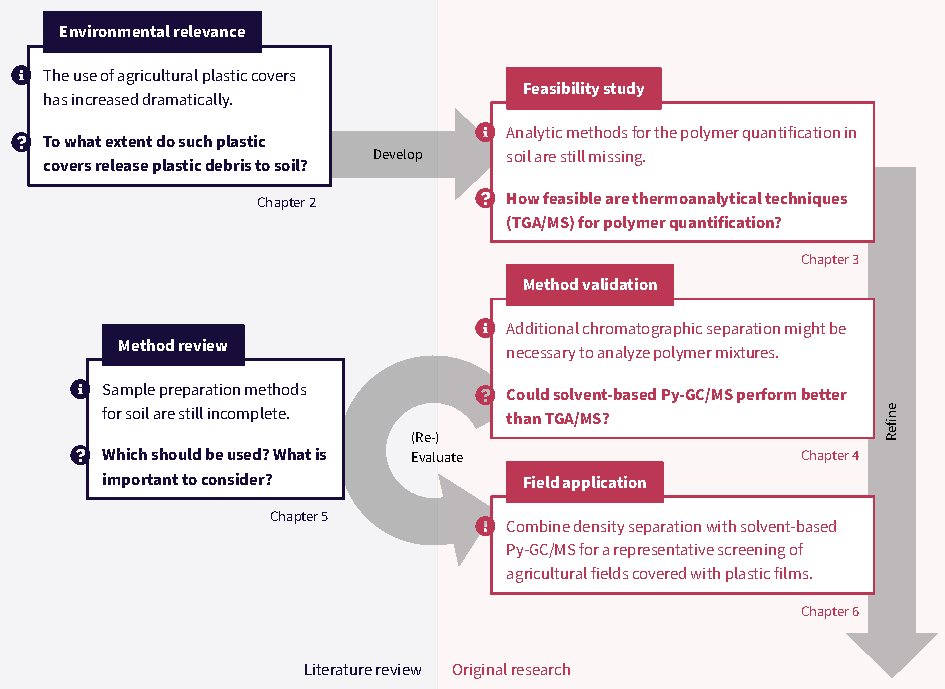
\includegraphics[width=\textwidth]{figures/thesis-overview}
	\caption{Conceptual overview and research questions addressed in this thesis.}
\end{figure*}

Objectives \ref{en:thermoanalysis} to \ref{en:application} were addressed consecutively as each objective relied on the outcome of the previous objective. Objective \ref{en:thermoanalysis} is covered in Chapter~\ref{ch:tga-ms-method}. This first proof-of-principle study used \ac{pet} as a model compound and one reference soil to investigate the potential of \ac{tga-ms} for plastic quantification. The method was designed to enable the rapid analysis of \SI{50}{\milli\gram} soil without any sample preparation. To facilitate the analysis of polymer mixtures and increase instrumental sensitivity, I continued method development using \ac{py-gc-ms} (objective \ref{en:chromatography}). However, \ac{py-gc-ms} is typically restricted to sample amounts \SI{<1}{\milli\gram} which poses high requirements on sample homogeneity. To overcome this and to reduce the risk of potential matrix interferences, I used \acf{tcb} to selectively dissolve \ac{pe}, \ac{pp}, and \ac{ps} in three different reference soils (objective \ref{en:dissolution}). This new solvent-based \ac{py-gc-ms} approach made up to \SI{4}{g} of soil amenable to the quantification of plastic debris (Chapter~\ref{ch:py-gc-ms-method}). Chapter~\ref{ch:analytical-techniques} critically (re-)evaluates this and other analytical techniques. With this knowledge at hand, I further refined my method for its subsequent application (objective~\ref{en:application}, Chapter~\ref{ch:screening}). This involved adjustments in the extraction mixture to increase polymer solubility and the addition of a suitable yet simple sample preparation technique to the existing \ac{py-gc-ms} approach. Thereby, plastic debris could be quantified from \SI{50}{\gram} soil. This sample amount was considered sufficiently large for a representative screening study of eight agricultural field covered with plastic films (Chapter~\ref{ch:screening}). Therein and in the following discussion (Chapter~\ref{ch:general-discussion}), I conclusively address the key hypothesis of this thesis and reflect on the implications of my findings.

% !TeX spellcheck = en_US

\chapter{Plastic Mulching in Agriculture}
\label{ch:plastic-mulching}

\paragraph{Abstract} Plastic mulching\marginnote{This chapter is based on: \fullcite{SteinmetzPlastic2016}.\par See \nameref{ch:author-contributions}, page~\pageref{ch:author-contributions}, for details.} has become a globally applied agricultural practice for its instant economic benefits such as higher yields, earlier harvests, improved fruit quality, and increased water use efficiency. However, knowledge of the sustainability of plastic mulching remains vague in terms of both an environmental and agronomic perspective. This chapter critically discusses the current understanding of the environmental impact of plastic mulch use by linking knowledge of agricultural benefits and research on the life cycle of plastic mulches with direct and indirect implications for long\-/term soil quality and ecosystem services. Adverse effects may arise from plastic additives, enhanced pesticide runoff, and plastic residues likely to fragment into micro- or nanoplastics but remaining chemically intact and accumulating in soil where they can successively sorb agrochemicals. The quantification of plastic debris in soil remains challenging due to the lack of appropriate analytical techniques. The cost and effort of recovering and recycling used mulching films may offset the aforementioned benefits in the long term. However, comparative and long\-/term agronomic assessments have not yet been conducted. Furthermore, plastic mulches have the potential to alter the soil quality by shifting the edaphic biocoenosis, accelerate \ch{C/N} metabolism eventually depleting \ac{som} stocks, increase soil water repellency, and favor the release of greenhouse gases. A substantial process understanding of the interactions between the soil microclimate, water supply, and biological activity under plastic mulches is still lacking but required to estimate potential risks for long\-/term soil quality. Currently, farmers mostly base their decision to apply plastic mulches rather on expected short\-/term benefits than on the consideration of long\-/term consequences. Future interdisciplinary research should therefore gain a deeper understanding of the incentives for farmers and public perception from both a psychological and economic perspective to develop new support strategies for the transition into a more environment\-/friendly food production.

\section{Introduction}
\label{sec:plastic-mulching:intro}

Rapid population growth poses a major challenge for both efficient and sustainable agricultural practices given the limited availability of arable land. In order to meet the increasing food demand \citep{GodfrayFood2010}, plastic mulching has become a widely used technique for its instant economic benefits such as higher yields and improved crop quality \citep{LamontPlastic1993}. However, after six decades of research\sidenote{See \citet{KasirajanPolyethylene2012} for an extensive historical review.}, the knowledge of the sustainability of plastic mulches remains vague in terms of both an environmental and agronomic perspective.

Plastic mulches are primarily used to protect seedlings and shoots through insulation and evaporation prevention, thus maintaining or slightly increasing soil temperature and humidity \citep{TararaMicroclimate2000}. Furthermore, the application of plastic covers is known to reduce weed and pest pressure \citep{McKenzieLandscape2001}. Often reported benefits are minimization of the development time for seed and fruit, yield increase, the prevention of soil erosion and weed growth, and consequently reduction of herbicide and fertilizer use \citep{Chalker-ScottImpact2007,EspiPlastic2006,LamontPlastic1993, Scarascia-MugnozzaPlastic2011}. These prospects have made plastic films an upcoming technology, nowadays making up by far the largest proportion of covered agricultural surface
in Europe (\SI{4270}{\square\kilo\meter}), an area four times larger than that covered by greenhouses and six times that of low tunnels \citep{Scarascia-MugnozzaPlastic2011}. While the agricultural surface covered with mulching films remains constant or shows only slightly growing trends throughout the world (\SI{5.7}{\percent} annual growth until 2019) \citep{TransparencyMarketResearchAgricultural2013}, the covering rate in China increased dramatically between 1991 and 2004 with a growth rate of \SI{30}{\percent} per year \citep{EspiPlastic2006}. The \citet{NationalBureauofStatisticsofChinaChina2012} reported a four-fold increase of plastic mulch use from \SIrange[range-phrase = { to }]{319}{1245}{\mega\tonne} between 1991 and 2011.

However, modifying the microclimatic conditions under plastic mulches not only enhances plant productivity but also increases biological degradation of litter and \ac{som}, which has recently been discussed as a trigger to rapid depletion of soil nutrients in general and carbon stocks in particular \citep{Domagala-SwiatkiewiczEffect2013,ZhangEffects2015}. This may eventually reduce soil quality in terms of impeding the soil's capability to serve its intended purpose \citep{DoranDefining1994}.
Furthermore, the excessive use of hardly degradable \ac{pe} has been apprehended to lead to substantial amounts of plastic waste residues accumulating each year \citep{AlbertssonMechanism1987}. This, in turn, may potentially release toxic additives into the soil \citep{RamosPolyethylene2015}.

The majority of reviews published on agricultural plastic mulching strongly focuses on the feasibility or efficacy assessments of biodegradable films \citep{BrodhagenBiodegradable2015,KasirajanPolyethylene2012} which have so far been hardly accepted as a functional alternative to \ac{pe}. More general contributions compared various synthetic and natural mulching materials with each other \citep{Chalker-ScottImpact2007,GreerAluminum2003} or with respect to certain agricultural practices, such as ridge\-/furrow systems \citep{GanRidgeFurrow2013} and integrated weed control \citep{BondNonchemical2001,CaseReview2005}. The first and most general reviews published on plastic mulching \citep{LamontPlastic1993,TararaMicroclimate2000} were animated with the beneficial prospects of plastic mulch use, however, merely discussing potential drawbacks. This trend still applies to the majority of current research articles emphasizing individual effects of plastic mulching with particular focus on short\-/term agronomic benefits \citep[for instance,][]{HeRice2013,Lopez-LopezWater2015,WangCombination2010}. In contrast, the long\-/term impact of plastic mulching as a standard agricultural practice is still virtually unknown in terms of potentially deteriorating soil quality or their post\-/crop fate, and therefore presents a challenge to bear a holistic sustainability evaluation. For this, it is important to combine the various results from individual studies to derive a system\-/based and interdisciplinary understanding of the processes governing the impact of plastic mulches on agroecosystems.

This review aims at evaluating the sustainability of plastic mulch use in agriculture from the perspective of soil biogeochemistry, environmental chemistry, agronomy, and society. We link current knowledge of agricultural benefits and research on the fate and life cycle of plastic mulches with direct and indirect implications of plastic mulching for short- and long\-/term soil quality. In this respect, we first outline the fate of \ac{pe} mulches while in use and after their life cycle has come to an end by explaining possible degradation pathways of buried mulch fragments. In addition to the fate of the plastic itself, we evaluate the long\-/term impact of plastic mulches on soil quality with respect to microbial diversity and \ac{som} composition and degradation, both important but often neglected factors influencing ecosystem functions \citep{PowerEcosystem2010}. On this basis, we assess the value of plastic mulches in an agronomic context in order to provide first insights into its sustainability. We finally identify the need of research for a better comprehension of the processes and factors influencing wanted and unwanted effects of agricultural plastic mulches.

\section{Methods}
\label{sec:plastic-mulching:methods}

We searched both Web of Science and Google Scholar literature databases for search terms including plastic or \ac{pe} mulch, cover, film, or tarp used in agriculture\sidenote{\sloppy Exact search string: \texttt{(plastic* OR \acl{pe}) AND (mulch* OR cover* OR film OR tarp) AND (soil OR agricultur*)}.}. Based on these findings and supplemented with cross references, we selected \num{572}~original research articles, \num{53}~reviews, \num{23}~books or book chapters, \num{21}~reports and doctoral theses, and \num{7}~patents and industrial standards for further evaluation. The literature covered the following major subtopics: use, properties, fate, impact on soil quality, and economic effects. For a more comprehensive perspective on the economics of plastic mulches we selected and followed the concept of ecosystem services \citep{MillenniumEcosystemAssessmentEcosystems2005} to identify economic elements linked to plastic mulching and to provide an integral overview of the current state of agronomic knowledge of the impacts of plastic mulch.

\section{Use and Properties of Plastic Mulches}
\label{sec:plastic-mulching:use-and-properties}

The largest benefits plastic mulches are used for on immense scales worldwide stem from their distinct optical and material properties that allow transmission or reflectance of specific wavelengths of incoming solar radiation \citep{BrownBlack2001,Chalker-ScottImpact2007,CsizinszkyColor1995,GordonPlastic2008,HaynesUse1987}. In order to produce highly customizable materials with high flexibility, durability, easy processing, and freedom from odor and toxicity \citep{WrightIns2019}, \ac{pe} has become by far the most frequently used base material in agricultural mulch production \citep{Diaz-PerezBell2010,KaraEffects2013,LocascioRed2005,SivanNew2011}. Its properties are usually modified by additives such as plasticizers, colored pigments, \ac{uv} stabilizers, or other polymers. The main types of \ac{pe} used in agriculture are low- and high-density \ac{pe} and linear low-density \ac{pe}.
High-density \ac{pe} is used to reduce weight and cost, contributes to the tear strength of the material, and provides a reliable moisture barrier \citep{LamontPlastics2005}. Linear low-density \ac{pe} is used for its elasticity and high puncture resistance \citep{AnthonyMultilayer1983}. Numerous other \ac{pe} mulching variations have already been patented, for instance composite mulches such as paper covered in styrene butadiene latex \citep{DalebrouxMulching1997}.
\citet{SabbaghAgricultural2010} patented a non\-/degradable and mechanically stable mulch barrier consisting of low-density \ac{pe}, linear low-density \ac{pe}, and \ac{pa}\slash nylon impermeable to soil fumigants. However, the degradability of such materials, the tendency to create microplastic debris, and their practical application are unknown. Mulches containing \ac{pvc} were prohibited for mulching in the US for their toxicity and carcinogenic potential \citep{USEPAGuidelines2012} and have been restricted to greenhouse covering and irrigation pipes \citep{Scarascia-MugnozzaPlastic2011}. In order to achieve longer life cycles of three years or more \citep{BrucknerSpargelanbau2008} as specifically needed for strawberries and asparagus growth, \ac{eva} and \ac{eba} are added to \ac{pe} mulches as copolymers \citep{EspiPlastic2006}.

Although this depends on regional climatic conditions and land use practices, maximum yields are mainly achieved by optimizing the amount of solar radiation absorbed by the crop. Further microclimatic parameters to be modified include the root zone and leaf temperature, humidity, and therewith soil moisture and plant transpiration rates, for example to manage soil temperatures at night or in colder regions by preventing evaporative cooling and emission of long\-/wave radiation from the soil \citep{HamOptical1993}. This is achieved by controlling the gas and heat exchange between the soil and the environment \citep{LamontPlastic1993,TararaMicroclimate2000}. For such purposes, black, transparent, and white mulches are the colors used most commonly. However, the color selection strongly depends on the crop type and the crop's environment, as well as the temperature that can be tolerated by plants and seedlings \citep{LamontPlastic1993,TararaMicroclimate2000}.

Black is the predominant mulch color since it can both absorb and re-emit radiation as thermal energy or long\-/wavelength \ac{ir} \citep{LamontPlastic1993,LamontPlastics2005}. Black mulch\-es are favored in moderate climate zones in order to increase soil warming by up to \SI{6}{\degreeCelsius} and double soil moisture, resulting in extended growing seasons. In very hot regions or for special use cases such as asparagus growing, white or white\-/on\-/black mulches are used to maintain or slightly lower soil temperatures by up to \SI{2}{\degreeCelsius} compared to bare soil \citep{HamOptical1993,HeissnerComparison2005}. The effects of plastic mulches on soil temperature and moisture typically decrease with soil depth, becoming mostly insignificant below \SI{40}{\centi\meter} \citep{Diaz-HernandezEffects2012,HeissnerComparison2005}. By contrast, transparent plastic films are poor absorbers of solar radiation but able to transmit \SIrange{85}{95}{\percent} of radiation \citep{HamOptical1993}. The condensed water below the film surface absorbs the \ac{ir} radiation reflected by the soil so that the heat is retained. This greenhouse effect makes transparent films profitable in colder regions \citep[for instance,][]{HaynesUse1987,StreckEffect1995}. However, the disadvantage of the high transmittance properties of transparent mulches is the lack of weed control, which continue to grow when exposed to sun light \citep{LamontPlastic1993}. In arid regions, transparent films are primarily used for soil solarization due to the extraordinarily high temperatures occurring under transparent mulches. Soil solarization is a soil sterilization method applied before planting to eradicate soilborne pathogens and devitalize weed growth \citep{HorowitzSolarization1983,TamiettiSoil2006}. In addition, photoselective films are capable of reflecting \ac{par} to above\-/film leaves and transmitting \ac{ir} light, representing a compromise between transparent and black mulches \citep{PaulUse2005}. For pest and pathogen control, pesticide \citep{SubrahmaniyanWeed2011} or aluminum \citep{CsizinszkyColor1995} coatings may additionally be applied\sidenote{See \citet{GreerAluminum2003} for a detailed overview.}. Other colors such as red, blue, yellow, or orange have also been tested for special requirements in vegetable production such as repelling certain pests or attracting beneficial insects \citep{CsizinszkyColor1995,LamontPainting1990, OrzolekUse1993}.

Apart from the evaluation of specifically intended effects of the variety of different plastic materials, none of the aforementioned studies focused on implications for other soil processes. In order to assess the impact of plastic mulching on soil quality, the current focus on the evaluation and optimization of the benefits of plastic mulching must be extended by the evaluation of potential unwanted side effects in soil and surrounding ecosystems. A comprehensive understanding of these effects will require an integrated assessment of application\-/specific impacts as well as process\-/orientated research on soil quality and the fate of mulch residues in soil that both the mulch and the soil are subjected to with respect to different environmental and agricultural conditions in particular regions of the world. In the following sections, we will thus discuss the current knowledge of these aspects.

\section{Fate of Plastic Mulches and their Additives}
\label{sec:plastic-mulching:fate}

\subsection{Life Cycle and Degradability of \Acs{pe}}
\label{sec:plastic-mulching:life-cycle}

A polymer is typically defined as ``environmentally degradable'' or ``biologically degradable'' if it has the ability to undergo disintegration, this is deterioration in mechanical properties, possible fragmentation, followed by microbial attack \citep{KrzanStandardization2006}. European standards further define that after six months more than \SI{90}{\percent} of the initial compound must be broken down to biomass, water, and \ch{CO2} \citep{DINEN13432Packaging2000}. In this sense, chemically inert \ac{pe} can be treated as virtually non\-/biodegradable \citep{AlbertssonMechanism1987}. Studies on the degradability of \ac{pe} have been recently reviewed in two articles \citep{KruegerProspects2015,Restrepo-FlorezMicrobial2014}. They reported that \ac{pe} degradation takes place to a certain extent. However, the authors agreed that this process is very slow under environmental conditions. Although the stability of \ac{pe} is beneficial for the lifetime extension of the mulch in use, this inertness is likewise the most problematic property concerning the disposal of used mulch films.

The typical application time of plastic mulches in agriculture lasts only a few months and can be reduced even further when exposed to extreme weather events such as hail and storms due to physical fragmentation and chemical aging processes \citep{Scarascia-MugnozzaPlastic2011}. More resilient mulches are required for perennial crops like strawberry or asparagus \citep{HablotEffect2014}. The thinner the film the more difficult and time consuming it becomes to remove the complete film from the field at the end of a crop cycle without leaving residues in the soil. For this reason, plastic films or parts thereof are often intentionally or unintentionally left on the field to be further broken down mechanically \citep{MorenoImage2014}.
Despite its high relevance, there is no information up to now on the amount of plastic residues in soil. However, \num{10}-year laboratory experiments showed that low-density \ac{pe} buried in soil reduced its weight by only \SI{0.2}{\percent} per year \citep{AlbertssonMechanism1987}. Long\-/term (\numrange{32}{37}~years) studies by \citet{OhtakeStudies1998} estimated a period of approximately \num{300}~years required for complete degradation of a \SI{60}{\micro\meter} thin low-density \ac{pe} layer. In pure \ac{pe} without any degradation\-/promoting additives, polymer chain scission is, if at all, a very slow process. \ac{pe} mulches are resistant to hydrolysis and are not readily attacked by microorganisms \citep{StevensGreen2002}. The most efficient way of chemical degradation involves a photo\-/oxidation step when exposed to sunlight. During this process, carbonyl groups are formed which can be attacked by microorganisms so that the polymeric chains are broken down further. These processes are summarized as oxodegradation, this is the fragmentation of plastic under the influence of \ac{uv} radiation and temperature \citep{SivanNew2011}. According to the definition of the American Society for Testing and Materials \citep{ASTMD5488-94Terminology1994}, such processes cannot be referred to as biodegradation since carbonyl formation during photo\-/oxidation is not an enzymatic activity. Moreover, mulching films that are buried in the soil are not subject to photo\-/oxidation and therefore unlikely to be attacked by microorganisms due to the lack of carbonyl formation \citep{MorenoImage2014}.

If not removed from the field, plastic waste accumulates in the environment where it may pose a considerable threat to terrestrial and aquatic wildlife when taken up in the food chain \citep{BarnesAccumulation2009,DuisMicroplastics2016,RilligMicroplastic2012,SivanNew2011,TeutenTransport2009}. Eventually, the plastic loses its integrity and breaks down into smaller and smaller particles for which the term ``microplastics'' was coined by \citet{ThompsonLost2004}. Although numerous articles have already reported the formation of plastic residues of various sizes (\SI{700}{\square\micro\meter} to \SI{2850}{\square\centi\meter}) originating from mulching \citep[for example,][]{BriassoulisAnalysis2015,FeuilloleyDegradation2005,KyrikouBiodegradation2007,RamosPolyethylene2015}, the assessment of their fate in soil is still challenged for the development of adequate analytical methods to detect and quantify plastic residues in complex, heterogeneous environmental matrices \citep{RilligMicroplastic2012}. Recently, \citet{DumichenAnalysis2015} suggested a first approach for the determination of \ac{pe} plastic debris in solid media using \ac{ted-gc-ms}. However, the authors stressed the need for further research in terms of improving \ac{ted-gc-ms} measurements as well as developing alternative techniques for the quantification of other polymer types in different environmental media.

The compiled findings suggest a successive enrichment of the plastic residues in the soil---whether or not they are left in the soil intentionally or unintentionally. For a more detailed assessment of the environmental fate of plastic residues, a more comprehensive understanding of the fate of plastic debris in soil is essential. This assessment, however, urgently requires further advances in analytical techniques to detect, identify, and quantify plastic debris in heterogeneous samples like soil.

\subsection{Phthalates}
\label{sec:plastic-mulching:phthalates}

Among typical \ac{pe} mulch additives, plasticizing agents from the group of \acp{pae} with its model compound \ac{dehp} belong to the most discussed soil contaminants \citep{FuUptake2011,MagdouliDi2013,WangSoil2013}. Similar to other \acp{pae}, \ac{dehp} is suspected of being carcinogenic and endocrine\-/disrupting \citep{ErkekogluGenotoxicity2014}. The fate of such compounds is highly relevant when assessing the risks potentially originating from plastic mulches. However, demonstrating a connection between plastic mulch application and elevated \ac{pae} concentrations in soil or plants is not trivial since agrochemicals, wastewater irrigation, and atmospheric background concentrations represent further potential \ac{pae} sources \citep{HongjunDistribution2013,WangSoil2013,HeContamination2014}. In \ac{pe} mulches, \ac{pae} are only loosely incorporated in the polymer structure without covalent bonding and can therefore be leached out easily. Even \ac{pae} derivatives with low water solubility, low vapor pressure, and high \acp{kow} such as \ac{dehp} \citep{MagdouliDi2013}, have been found ubiquitously in the environment \citep{FernandezOccurrence2012}. While typical background concentrations of \acp{pae} in soil vary between \SIrange[range-phrase = { and }]{0.2}{33.6}{\milli\gram\per\kilo\gram} \citep{ZengPhthalate2008}, \ac{pae} levels in plastic mulches were detected in ranges from \SIrange[range-phrase = { to }]{50}{120}{\milli\gram\per\kilo\gram} \citep{WangSoil2013}.
Plastic\-/mulched crop land revealed concentrations of six major \acp{pae} between \SIrange[range-phrase = { and }]{74}{208}{\percent} higher than in non\-/mulched farmlands in China \citep{KongDiversities2012}. Most concentrations of \ac{dehp} and \ac{dbp} found in Chinese\-/grown vegetables and soil exceeded US and EU food security standards and environmental risk limits of \SIlist{0.7;1.0}{\milli\gram\per\kilo\gram}, respectively \citep{vanWezelEnvironmental2000,WangOccurrence2015}.

Once released from the mulching film, \ac{pae} may be distributed in environmental compartments by plant uptake, evaporation into the atmosphere, and runoff into groundwater and surface waters \citep{HeContamination2014}. In soil, \ac{pae} are degraded by microorganisms to different extent in dependence of the ester chain length. While short\-/chain esters, such as \ac{dep}, are to a certain extent susceptible to biodegradation, longer chains as in \ac{dehp} render the \ac{pae} persistent. When subjected to \ac{uv} radiation, \acp{pae} can degrade to phthalate monoesters and phthalic acid \citep{HankettMolecular2013}. In natural environments, the governing microbial degradation processes are hydrolysis, both aerobic and anaerobic, followed by aromatic ring cleavage \citep{MagdouliDi2013,StaplesEnvironmental1997}. Furthermore, microbial degradation of \acp{pae} is dependent on its metabolic yield: Whereas \ac{dep} is rapidly degraded and assimilated, \ac{dehp} and bis(2-ethylhexyl) adipate are more recalcitrant and only cometabolically degraded in the presence of an additional carbon source \citep{CartwrightDegradation2000,NalliBiodegradation2002}. This typically results in the formation of ethylhexanoic acid and ethylhexanol, both toxic to aquatic organisms and particularly resistant to further degradation \citep{HornPlasticizer2004}. Although laboratory\-/derived half lives of \acp{pae} in soil range from days to months, current research rather suggests that at least some of them persist for significantly longer periods in soil \citep{RudelDegradation1993}. Thus, the use of plasticizer\-/containing mulches involves a clear potential for accumulation of these xenobiotics in soil and a successively increasing risk of bioaccumulation and biomagnification in the food web.

Besides affecting the abundance and diversity of soil organism communities, crop quality can be impaired significantly when \acp{pae} are taken up by plants \citep{KapanenPerformance2008,WangOccurrence2015}. Through this pathway, phthalates may eventually enter the food supply chain representing an additional and probably significant source of exposure to humans.

\subsection{Polymer Degradation-Promoting Agents}
\label{sec:plastic-mulching:oxodegradation}

Due to the generally known high persistence of plastic residues and their additives in soil, the development of biodegradable plastics or the promotion of biodegradation of plastic materials is a promising option to avoid the accumulation of plastic in soil. First attempts were made to use different bacterial strains, for example from the gut of the Indian meal moth (\latin{Plodia interpunctella}), which were able to degrade \SIrange{6}{10}{\percent} \ac{pe} during a \SI{60}{\day} incubation period \citep{HadadBiodegradation2005,KruegerProspects2015,YangPlastic2015}. However, such selective treatments have been restricted to laboratory conditions. They seem both too difficult and expensive to be applied on large agricultural scales and bear the risk of potentially introducing invasive or detrimental species into productive systems. Certain agrochemicals, such as paraquat and mancozeb were found to accelerate the oxidation rate and embrittlement of the \ac{pe} foil during laboratory experiments, while sulfur and chlorpyrifos did not show significant effects \citep{YehEffect2015}. By contrast, various types of other \ac{pe} additives have already been successfully tested and applied for their ability to promote the breakdown of mulches. \Citet{KyrikouBiodegradation2007} provided a comprehensive collection of data on various types of mulches and investigated under which conditions and to which extent they are (bio)degradable. In order to promote oxodegradation, additives can be used to facilitate chain cleavage and microbial attack. Polymer breakdown is induced by radicals produced by pro\-/oxidants and the subsequent production of oxidized carbon chains \citep{BriassoulisDegradation2015}.
Such pro\-/oxidants mainly contain carbonyl groups and compounds containing transition metals like \ch{Fe}, \ch{Co}, and \ch{Mn} \citep{KyrikouBiodegradation2007}. However, added organic compounds or metals of environmental concern may lead to increasing soil contamination \citep{KoutnyBiodegradation2006,Scarascia-MugnozzaPlastic2011}. It has not yet been satisfactorily shown to what extent the oxidation products are truly biodegradable under realistic environmental conditions. In several standardized laboratory biodegradability tests, less than \SI{2}{\percent} of a pro\-/oxidant\-/containing \ac{pe} mulch was degraded over a two-year period \citep{FeuilloleyDegradation2005}. Comparable results were shown in a \num{7}-year field experiment after exposing pro\-/oxidant\-/containing linear low-density \ac{pe} films to enhanced \ac{uv} radiation and heat in the laboratory. The results suggested a predominance of mechanical rather than chemical breakdown in soil and a successive formation of microplastics invisible to the naked eye \citep{BriassoulisDegradation2015}. In another field study (\num{8.5}~years), linear low-density \ac{pe} mulch films containing pro\-/oxidants exhibited a degradation in mechanical properties due to the formation of carbonyl groups during the cultivation period, but they did not disintegrate chemically. After the cultivation period, the almost intactly recovered films successively decreased in carbonyl groups, possibly due to leaching of carboxylic acids by soil water, which reduces available sites for microbial attack even further \citep{BriassoulisAnalysis2015}. This leads to the hypothesis that pro\-/oxidant\-/containing mulches undergo fragmentation but are not subject to subsequent microbial degradation, so that they accumulate in the soil as polymers of reduced chain length. Therefore, such films can be classified neither as biodegradable nor as environmentally degradable according to the definition given above. Although referred to ubiquitously, the definition of ``biodegradable'' does not necessarily state an approximate period of time for biodegradation by which plastic can be accepted as such. A reasonable time frame for complete degradation would be until the beginning of the new crop cycle in order to avoid plastic fragments and additives being incorporated into the soil.

The compromise between the need to sustain the mulch's property during use and the requirement to be rapidly biodegraded after use remains a major challenge for material science. This is further aggravated by the requirement that biodegradation must take place in the field, under less well\-/defined and less optimal conditions than performed in standard degradation tests. Thus, up to now, it seems open whether in the future truly biodegradable mulching films will be available for application in agriculture.

\subsection{Disposal and Recycling of Used Plastic Mulches}
\label{sec:plastic-mulching:recycling}

The fate of plastic mulches not only deals with fragments buried in the soil, but also with plastic waste collected from the field. Its disposal represents a task both laborious and costly. When removed from the field, one of the major problems in plastic disposal and recycling is its contamination with soil and agrochemicals \citep{Gonzalez-SanchezUse2014,Scarascia-MugnozzaPlastic2011}.
In Europe, regulations concerning landfilling vary considerably between countries. While in Central Europe and Scandinavia (excepting Finland) less than \SI{10}{\percent} of both agricultural and non-agricultural plastic waste is disposed of in landfills or landfill bans are implemented, in Spain and most eastern and southeastern countries more than \SI{50}{\percent} of plastic waste are estimated to be landfilled \citep{PlasticsEuropePlastics2015}. However, contaminated mulches are mostly unsuitable for landfilling due to the risk of pesticide leaching \citep{GartheManaging2004,WangSoil2013}. \ac{pe} sheets may even function as a vector and facilitate transfer of pesticides into the soil by absorbing the pesticide in the non\-/crystalline areas of the film \citep{HuckinsLipidcontaining1993,NerinAbsorption1996} and further migration of the pesticide to the soil matrix \citep{RamosPolyethylene2015}. The decreasing space available for landfills and concerns over the disposal of contaminated plastic render incineration of plastics a viable alternative, especially for power production \citep{GartheManaging2004}. High\-/temperature combustion (\SI{>1000}{\degreeCelsius}) of \ac{pe} and \ac{pvc} produces as emission products mainly the ozone\-/damaging greenhouse gas \ch{CO2}, \ch{CO}, and polycyclic aromatic hydrocarbons \citep{WangComparative2003}. Illegal on\-/site burning of halide\-/containing plastics may even release carcinogenic dioxins at levels 20 times that of controlled high temperature incineration and 40 times that of atmospheric particulate matter \citep{LevitanRecycling2003}.

A desired alternative to landfill disposal and incineration is the recycling of used mulching films. In 1991, a patent application was filed that proposed the use of a recycling machine designed for cleaning and shredding agricultural plastic waste \citep{VacchelliAnlage1992}. However, no information is available whether such machinery was or is being used at some point. This may imply that the cost and effort exceed the benefits of small\-/scale recycling machines. Recycling used mulch is only possible if contaminants make up less than \SI{5}{\percent} of the total weight of the mulch \citep{ClarkeRecycling1996}. Studies have shown that this \SI{5}{\percent} threshold is exceeded dramatically with the actual contaminant weight being up to \SIrange{40}{50}{\percent} \citep{HussainPlastics2003, LevitanRecycling2003,NerinAssessing1999}. This leaves large amounts of mulching films not being recycled at all---a problem scarcely stressed in the scientific literature but in a US newspaper for agricultural operators \citep{KotrbaWhat2008}.
Also, the \citet{EUWasteFrameworkDirectiveDirective2008} does not specify disposal or recycling procedures concerning agricultural plastic waste. Since plastic disposal in an environmentally safe manner is more recommendatory than effectively implemented in terms of regulations both in the US and the EU, the fate of used plastic mulches is largely unknown.
For want of alternatives, farmers may dispose of the waste through illegal on-site burning or unsuitable pits \citep{HemphillAgricultural1993, Scarascia-MugnozzaPlastic2011}. In the UK, for example, only two
plants are known to reprocess agricultural plastic waste, which makes the collection of the mulch and transport to the plant excessively costly for remote and small\-/scale operators \citep{ScottishExecutiveEnvironmentGroupCode2006}. In Germany, the environmental agencies of the federal states list the temporary storage and disposal of used mulch in the statement of costs for vegetable farmers \citep{BayerischeLandesanstaltfurLandwirtschaftFeldgemuseanbau2005}. Although no precise instructions have been established for mulch disposal in Germany, transport to reprocessing plants appears to be common practice \citep{StraeterAlles2011}.

The lack of recycling options has led to the development of mulch materials which are completely free from plastic, like paper mulch mats made of recycled waste paper (EcoCover) which has, however, not produced any company\-/external research. Even the development and use of fully biodegradable plastic would not be without negative effects: \citet{GerngrossCan1999} argued that the life cycle of fermentation\-/derived polymers, for example from paper or corn starch, could be considered non\-/sustainable and environmentally more harmful than that of conventional plastic films due to side effects such as air acidification, eutrophication, and increased carbon emissions. Vegetable mulches from straw, coconut, or other barks further pose an increased hazard of pests which would be more detrimental than beneficial to crop production \citep{HowardOrganic1998}. Moreover, organic mulches cannot provide resistance to extreme weather conditions as plastic mulches can, and inconsistent weather conditions may lead to degradation or disintegration of the mulch before the end of the crop cycle and, thereby, to a high variability in plant growth and yield. Moreover, exotic mulches like coconut bark are only available in small amounts and certain areas of the world which makes their purchase a highly costly and laborious matter \citep{BriassoulisDegradation2015}.

In summary, the overarching problem of agricultural plastic waste remains the requirement to dispose of large quantities of used mulching films that are difficult to collect, recycle, and reuse. Besides the accumulation of chemically resistant \ac{pe} itself, the leaching of mulch additives and sorbed agrochemicals is of particular concern regarding soil contamination and impaired soil quality. According to our knowledge, only one life cycle assessment on \ac{pe} mulching has been published so far, and particularly focused on different soil and pest management techniques in an olive plantation \citep{RussoEnvironmental2015}.
In comparison with mulching with de-oiled olive pomace\sidenote{This is the solid waste product from olive oil mills.}, nonwoven \ac{pp} fleece, \ac{pe} foil, chemical and mechanical weeding, \ac{pp} and \ac{pe} mulches produced the lowest environmental burdens in total including plastic production, installation, collection, transport, and disposal. However, they scored worse in primary energy demand and the potential of volatilizing organic compounds to create photochemical ozone. \Citet{RussoEnvironmental2015} further stated that not all environmental impacts of agricultural practices are actually assessable by the current methodology of life cycle assessments and called for a longer\-/term soil monitoring when mulching techniques are applied. Long\-/term life cycle assessments should further include the most frequently used plastic mulch materials in order to better and more quantitatively judge the potential risks of plastic mulch applications. In addition to the risks originating from the plastic materials and its additives, knowledge of the impact of plastic mulching on soil quality is crucial. This aspect will be discussed in the following paragraphs.

\section{Impact of Plastic Mulches on Soil Quality}
\label{sec:plastic-mulching:soil-quality}

\subsection{Soil Porosity and Water Transport}

Surface covering prevents mechanical perturbations in the topsoil, such as from tillage, rainfall, or crust forming \citep{KhanSoil2000,SubrahmaniyanCrop2006}. Due to the isolation from direct natural water recharge, covered soil is particularly dependent on lateral water transport \citep{LiOpenHole2003} and often requires irrigation. However, once
irrigation is applied, plastic mulching typically increases the water use efficiency by \SIrange{20}{60}{\percent} due to reduced evaporation \citep{QinSoil2015,ZribiEfficiency2015}. Plastic mulches impede the gas exchange between the soil and the atmosphere \citep{KhanSoil2000}. Both gas and water transport can be managed using perforated plastic sheets.
However, the desired effects of increased temperature and moisture conditions on the soil surface are typically less pronounced than under closed synthetic covers \citep{LiOpenHole2003}. The same applies to so called ``biodegradable'' mulches which have a higher permeability due to gradual disintegration on site \citep{MorenoEffect2008}.

The mechanical protection of surface soil, together with an enhanced root development, mucilage production, and soil fauna activity, promotes the stabilization of soil aggregates \citep{SixHistory2004}. This is apparent in a shift in aggregate size distribution towards large (\SIrange{2.5}{4.0}{\milli\meter}) and water stable aggregates following mulching \citep{Domagala-SwiatkiewiczEffect2013,ZhangRunoff2013}. The increase in aggregate size is accompanied by a slight decrease in soil bulk density, consequently reducing soil compaction \citep{MbahPhysical2010,TindallMulch1991}. Both effects are associated with increased pore sizes and soil aeration \citep{KhanSoil2000}, feeding back positively to root development and soil biota activity \citep{SchonbeckEffects1998a}. The resulting loose and friable soil structure further allows an increased water holding capacity \citep{Domagala-SwiatkiewiczEffect2013,MbahPhysical2010} and reduces vertical water transport \citep{PeeyushEffect2008}. A higher water use efficiency decreases irrigation requirements and thereby the risk of soil salinization \citep{DongFurrow2008} and leaching of nutrients \citep{KimSimulation2014}, fertilizers \citep{HaraguchiEffect2004}, and pesticides \citep{LeibDrip2000}. Arid and sandy topsoil, however, may generally become dry or even hydrophobic under artificial or deficit water supply in a long\-/term perspective \citep{JaramilloOccurrence2000, RobinsonComparison1999}. Drying of soil hydrogels like mucilage can lead to a further increase in soil water repellency \citep{AhmedDrying2016,CarminatiRhizosphere2013}. In such cases, sealing the soil off from rainfall makes it more likely to lose potential benefits of an increased water holding capacity. However, it is still unclear under which conditions processes inducing soil water repellency or processes reducing water holding capacity are favored. For this, a comprehensive mechanistic understanding of the processes affecting soil wettability is required in order to judge the relevance of this risk. Up to now, the mechanisms and factors leading to soil water repellency are still under discussion \citep{DiehlSoil2013}.

Contrary to the water retention underneath the films, the surface of mulched ridges enhances water runoff into furrows which are particularly susceptible to soil erosion and loss of soil structural stability \citep{RiceRunoff2001,WanRunoff1999,ZhangRunoff2013}. The study by \citet{RooseOrganic2001} showed that the positive aspects of plastic mulching on soil structure do not necessarily express in all types of soil: Applying plastic mulch to an already heavily degraded nutrient\-/deficient and previously uncovered arid soil only temporarily reduced erosion. In contrast, the measure created even more fragile soil structures in the long term. In this case, natural attenuation processes may have already been lastingly deteriorated a priori so that negative effects of plastic mulching, such as inducing water repellency or an increased erosion potential, could no longer be compensated.

\subsection{Impact of Plastic Mulching on the Fate of Agrochemicals and Metals}

As discussed before, plastic mulching may significantly increase the mean runoff and soil loss from the field, especially to furrows \citep{WanRunoff1999,ZhangInfluences2014,ZhangDistribution2015}. Accordingly, total pesticide loads are often found elevated around plastic\-/mulched fields compared to bare soil or organic mulches. This poses the risk of pesticide runoff into the environment where they may adversely affect both aquatic and soil organisms \citep{ArnoldRunoff2004,DietrichFate2014}. For instance, runoff from \ac{pe} films increased chlorothalonil and $\alpha$- and $\beta$\-/endosulfan by \numlist{19;6;9} times, respectively, with respect to the hairy vetch\-/mulched control \citep{RiceRunoff2001}. The same research group observed up to \num{8} times higher runoff volumes containing the pesticides chlorothalonil, thiodan, endosulfan, and esfenvalerate from \ac{pe} mulch than from bare furrows \citep{RiceEvaluation2007}. Similar results were observed in a pineapple cultivation with the nematicide bromacil \citep{AlaviEvaluation2007}. Higher levels of dissolved copper and metolachlor were measured in the runoff water coming directly from covered tomato crops \citep{ArnoldRunoff2004,RiceComparison2002}. \Citet{FenollSolarization2010} reported that soil solarization promoted fungicide dissipation from soil. Furthermore, some studies showed an increased uptake of toxic metals by plants covered with plastic mulch: \citet{MorenoAccumulation2002} observed increased toxic metal accumulation in the aboveground plant biomass of Chinese cabbage; with total contents of \ch{Zn}, \ch{Cd}, \ch{Cu}, and \ch{Pb} elevated by up to \SI{90}{\percent} compared with uncovered plants. Potato plants mulched with \ac{pe} extracted up to three times more metals than uncovered treatments which, in turn, decreased soil metal contents \citep{BaghourInfluence2001,BaghourInfluence2002}. These and other soil processes will be discussed in the following paragraph.

\subsection{Soil Biological Metabolism and Diversity}

Given a sufficient nutrient supply and the absence of toxicants, elevated temperatures and soil moisture increase soil biological activity \citep{SubrahmaniyanCrop2006} and metabolism \citep{LiProductivity2004}. \ch{CO2} originating from soil respiration can be retained by \ac{pe} covers and acts as fertilizer for daytime photosynthesis when slowly diffusing through the plastic films itself or through holes punched for stems. This may lead to an enhanced carbon sequestration by \SIrange{12}{15}{\percent} \citep{AnCarbon2015} and reduced \ch{CO2} emissions into the atmosphere by approximately \SI{100}{\gram\per\square\meter} \ch{C} despite up to three-fold higher \ch{CO2} concentrations in mulched soils \citep{LiCarbon2011}. Promoted plant growth through \ch{CO2} fertilization may further stimulate root development and increase the exudation of mucilage. Nutrient uptake and availability for soil microorganisms will also be enhanced thereby \citep{LiuResponse2015,SubrahmaniyanCrop2006}, particularly in the rhizosphere \citep{LinEffect2008,MaulMicrobial2014}. As a consequence of an increased nutrient uptake and plant metabolism, phenolic compounds, flavenols, and vitamins were found to be increased, for instance in North American carrot and grapevine cultivations \citep{AntoniousColor2002,CoventryReflective2005}.
As discussed before, increased mineral uptake may also include the uptake of potentially co\-/present contaminants which has to be accounted for in terms of concerns over food safety \citep{MorenoGrowth2003}.

While \SIrange[range-phrase = { to }]{25}{60}{\percent} of soil carbon may be retained in microbial biomass \citep{AnCarbon2015}, the remaining accessible fraction can undergo metabolism \citep{ZhouRidgefurrow2012}. The impeded gas exchange through \ac{pe} mulches can furthermore induce suboxic soil conditions, resulting in redox potentials below \SI{-200}{\milli\volt} \citep{BlokControl2000}. Anoxic redox conditions of \SI{-500}{\milli\volt} have been reached in non\-/flooded, water\-/saving ground cover rice production systems \citep{KreyeFluxes2007}. Such low redox potentials first lead to impaired nitrification or increased denitrification and further promote methanogenesis, ultimately increasing \ch{N2O} and \ch{CH4} emissions \citep{AkiyamaEffect2003,KimSimulation2014,LiEffects2014}. Under oxidizing conditions, increased \ch{N2O} fluxes resulting in an increased global warming potential by up to \SI{80}{\percent} were observed predominantly during and after solarization and disinfection measures, or when the soil was fertilized substantially with inorganic nitrogen of \SIrange{300}{1600}{\kilo\gram\per\hectare} \ch{N} \citep{ArriagaGaseous2011,CuelloImpact2015,NishimuraNitrous2012}. Plastic mulching for its yield\-/increasing purpose together with moderate fertilization (\SI{<180}{\kilo\gram\per\hectare} \ch{N}), in contrast, mostly led to \ch{N2O} emissions comparable to those of non\-/mulched soil, for instance planted with radish and cotton in South Korea and China, respectively \citep{BergerPlastic2013, LiEffects2014}. For a reliable risk estimation of the contribution of mulched soils to the emission of climate relevant gases, a comprehensive understanding of the interactions between oxygen availability, soil temperature, crop and soil moisture is required. Such knowledge is, however, still incomplete \citep[see for example][]{Butterbach-BahlNitrous2013,SignorNitrous2013}.

Along with alterations in physical properties, soil nutrient availability, and microbial activity, plastic mulching can induce shifts in the soil microbial community \citep{HasegawaNitrate2004,MaulMicrobial2014}, for instance towards mycotoxigenic fungi \citep{MunozEffect2015}. Soil solarization practices were reported to generally decrease bacterial and fungal richness by favoring thermophilic, facultatively anaerobic and detritivorous species \citep{BonanomiSoil2008,SimmonsCharacterization2014}. This means that soil solarization is to a certain extent non\-/selective, particularly when applied in combination with soil fumigation \citep[for instance,][]{ChellemiFumigant2013}. Contrarily, ordinary plastic mulching for its yield\-/increasing purpose led to no significant decreases \citep{KapanenPerformance2008} or even slight increases in total microbial diversity compared to non\-/mulched soil \citep{ChenMulching2014, LiuRapid2011}. In this respect, organic or vegetative mulches alone or in combination with plastic mulches were shown to perform considerably better than plastic mulches \citep{CarreraEffects2007,MaulMicrobial2014}. Additional nutrient input and a more diverse habitat structure as provided by organic material was likely to increase soil microbial abundances and diversity \citep{DoganEffect2013,MunozEffect2015,SchonbeckEffects1998a}. However, first studies on the use of plastic mulch in asparagus crops suggested a risk of increased mycotoxin production in soil, this is deoxynivalenol \citep{MunozEffect2015}. If this observation holds further verification, the implications of plastic mulching for mycotoxin production and food contamination by mycotoxins need to be considered in future research as well.

The effects of plastic covers on soil microbes can propagate in different ways to higher trophic levels of the food web, for example by positively affecting overall arthropod diversity and doubling omnivorous insect abundance but decreasing springtail \citep{AddisonInitial2013}, predatory nematode \citep{ForgeEffects2003}, ground beetle \citep{MinarroEffects2003}, or earthworm abundances \citep{SchonbeckEffects1998a} by factors of \numrange[range-phrase = { to }]{2}{3}. The latter are of particular importance for maintaining a loose soil structure. Besides the partial information on specific scenarios, the overall impact of plastic mulching on the microbial biocoenosis, their functional diversity as well as their influence on nitrogen and carbon degradation and on the food web has been widely neglected, and remains only partially understood. With respect to the resilience of agroecosystems, it may be helpful to understand the impact of plastic mulching over time on the most relevant ecosystem functions related to soil biology and microbial diversity. Furthermore, it will be important to assess which conditions favor or suppress the development of potentially pathogenic microorganisms and mycotoxin producing fungi.

\subsection{\Acs{som} Composition and Stability}

Regardless of differing regional conditions or cropping scenarios, the enhanced productivity under plastic mulches has often been reported to result in lower contents of \ch{Mg}, \ch{K}, \ch{P}, and \ch{N} when compared to bare soil \citep{Domagala-SwiatkiewiczEffect2013,LiInfluence2007,SchonbeckEffects1998a}. Furthermore, \citet{MorenoEffect2008,LiDynamics2004,LiInfluence2007,ZhangEffects2015} found significant \ac{som} losses within one to three years of mulching due to temperature\-/induced, accelerated biodegradation, which were closely linked and intertwined with decreasing \ch{C/N} ratios \citep{JiaDynamics2006,ZhouRidgefurrow2012}. Higher temperatures, as required for soil solarization, may even deplete up to \SI{85}{\percent} of soil carbon in less than one month \citep{SimmonsManaging2013}. By contrast, \ac{som} contents remained stable during one to two years of plastic mulching when the soil carbon pool was maintained by organic matter input from crop residues or additional vegetative mulching \citep{SchonbeckEffects1998a,TindallMulch1991}. These effects are most probably due to the generally high temperature sensitivity of \ac{som} decomposition processes \citep{LarionovaEffect2014, vonLutzowTemperature2009}. \Citet{GanRidgeFurrow2013} hypothesized that such a decrease in \ac{som} is only temporary and would be compensated by the carbon input from root residues after some crop rotations. This is supported by recent findings by \citet{LuoSensitivity2015}, who showed that the carbon stocks decreased only in the top soil (\SI{<20}{\centi\meter} depth), but increased in the rooting zone (\SIrange{20}{40}{\centi\meter} depth) after four years of plastic mulching. However, it is still unknown under which conditions and to what extent changes in \ac{som} contents are governed, rather by an increased net primary production or by accelerated microbial decomposition. This knowledge is particularly relevant for carbon storage estimates in intensive land use scenarios and agricultural practices in which the majority of plant material is removed at harvest \citep{ChapmanSoil2012,PardoCultivationInduced2012,TianEffects2012}. For soils with limited natural carbon input, \citet{ZhangEffects2015} recommended a strict \ac{som} budgeting to avoid soil degradation.

Besides alterations in \ac{som} quantity, it remains largely unresolved how the potentially accelerated turnover of soil \ac{Corg} may affect \ac{som} structure \citep{DiaconoLongterm2010}. This extends to the temporal development of \ac{som} quality under plastic films in terms of maintaining its benefits for agricultural soil use in a long\-/term perspective \citep{DoranDefining1994} and, possibly even more important, its ecosystem functions. In general, the rapid soil respiration and mineralization, soil erosion, and leaching \citep{BolanDissolved2011} are known to impede \ac{som} humification and to reduce \ac{som} stability \citep{SollinsStabilization1996} and are thus suspected to reduce overall soil quality \citep{LalChallenges2009}. Contrary to that, the formation of larger soil aggregates mediated by plant residues and soil biota can stabilize \ac{som} by increasing the amount of organic matter spatially inaccessible to microbial attack \citep{SollinsStabilization1996,vonLutzowStabilization2006}. This humified \ac{som} acts as an important binding agent on the microscale through the formation of organo--clay and mineral complexes which may favor soil structural stabilization on the macroscale \citep{BronickSoil2005,ZhangEffects2015}.

Under mulched soils, information on \ac{som} formation and degradation processes is often estimated from microbial respiration rates \citep{LiDynamics2004,MorenoEffect2008}. However, such proxies do not provide any information on the change in \ac{som} composition and \ac{som} structure. To our knowledge, there is only one study so far which assessed in detail changes in \ac{som} structure and quality following plastic mulching: \citet{CeccantiPyrolysisgas2007} analyzed mineralization indices (furfural\slash pyrrole\slash phenol ratios), humification indices (benzene\slash toluene), and aliphatic\slash aromatic ratios before and after four months of \ac{pe} mulching by means of pyrolysis\-/gas chromatography.
The obtained indices indicated no difference between \ac{pe}\-/mulched compared to bare or fertilized soil. In contrast to this detailed but short\-/term experiment, long\-/term effects of multiannual plastic mulching on \ac{som} composition have often been reported in less detail. Those studies mostly used density fractionation techniques to address differences between the
light or labile \ac{som} fraction containing low\-/density, easily degradable, but temporarily not yet completely decomposed organic material such as roots and leaf litter and the heavy or stable \ac{som} fraction \citep{SollinsNet1984}. Although this classification is merely operational, the light fraction is known to have residence times of a few years to several decades \citep{vonLutzowStabilization2006} and is therefore adduced as a sensitive indicator for changes in \ac{som} induced by land use \citep{JanzenLightFraction1992}. \Citet{LiuEffects2013,LuoSensitivity2015,ZhouRidgefurrow2012} reported up to two-fold increases of readily available labile carbon after two to four years of plastic mulching; all using the same fractionation scheme. This trend was similarly reflected by a \num{10}-year study in which a mulched soil cultivated with non\-/flooded rice and wheat revealed \SIrange{50}{60}{\percent} more labile dissolved organic matter compared to uncovered soil \citep{TianLabile2013}. Slight increases in both light and heavy \ac{som} fractions under mulch were only reported for an alfalfa grassland in China \citep{JiaDynamics2006}. Although not been studied in further detail with respect to plastic mulching, information on the implications of alterations in the \ac{som} development can be deduced from studies on other soils: If not removed at harvest, the light fraction may be incorporated into \ac{som} and promote the accumulation of more stable and humified \ac{som} structures \citep{ZhouRidgefurrow2012} with narrower \ch{C/N} ratios \citep{SollinsNet1984}, or it may be incorporated into soil aggregates, where it is protected physically from microbial attack \citep{SollinsStabilization1996,vonLutzowStabilization2006}, as discussed above. Under natural conditions, this intermediate to stable \ac{som} fraction has an estimated residence time of hundreds to several thousands of years \citep{vonLutzowStabilization2006}, however, its stability and resistance towards mineralization are particularly more sensitive to temperature changes ($Q_{10} = 4.3$) than the corresponding fraction of labile \ac{som} ($Q_{10} = 2.4$) \citep{LarionovaEffect2014,vonLutzowTemperature2009}. At a mean temperature of \SI{22}{\degreeCelsius}, this may result in a mean lifetime\sidenote{This is the reciprocal of the decay constant.} of stable \ac{som} reduced to \num{35}~years \citep{LarionovaEffect2014}. Moreover, elevated contents in labile carbon have been hypothesized to potentate stable \ac{som} breakdown \citep{GuenetEvidence2012}. Both aspects can lead to an increased degradation of the intermediate to stable \ac{som} fraction. Thus, the current general knowledge of stabilization and destabilization mechanisms of \ac{som} suggests that the processes under plastic mulch favor degradation and destabilization of \ac{som}. With regard to the long residence times of stable \ac{som}, a mulching\-/induced decrease in this \ac{som} fraction is likely to persist even when the measure has stopped. However, these hypotheses still need to be verified with respect to plastic mulching.
Here, it will be important to study the interaction between the enhanced stabilization of organic matter by aggregates on the one hand, and the enhanced potential to be degraded due to higher temperatures and modified soil moisture on the other hand. This requires a process\-/orientated mechanistic knowledge of the \ac{som} degradation processes under the conditions of plastic mulching.

Although comprehensive evidence on the further long\-/term development and recovery potential of \ac{som} structures and quality under plastic mulch is still missing, all current findings point into the same direction: Multiannual plastic mulching favors the formation of labile organic matter or degradation of intermediate to stable organic matter. This can be regarded as an alarming indicator for decreasing soil quality and may constitute a potential risk of the soil becoming a \ch{CO2} emittent. The accelerated soil processes under plastic mulch can thus be deemed a major driver altering \ac{som} composition and quality \citep{SchmidtPersistence2011,vonLutzowTemperature2009}. This involves
\begin{enumerate*}
	\item increased soil metabolism and mineralization, particularly of stable \ac{som} structures,
	\item rapid nutrient turnover and
	\item soil aging,
\end{enumerate*}
this is degradation in soil quality. Since photosynthesis has a lower temperature sensitivity than degradation kinetics \citep{KirschbaumWill2000}, it seems unlikely that a mulching\-/induced accelerated net primary production may compensate or overbalance net \ac{som} degradation. However, this relation is currently largely unknown.

Even though most \ac{pe}\-/mulched soils are still comparatively young and fertile, low carbon stocks and degraded \ac{som} are well known characteristics of weathered soils located in regions with high mean annual temperatures, as is, for example reported for soils in the tropics or those expected to be subjected to global warming \citep{DavidsonTemperature2006}. Many of such soils are characterized by a labile, highly dynamic equilibrium between rapid organic matter supply and rapid degradation with a lower relevance of organic matter stabilized by minerals \citep{ZechFactors1997}. Once this fragile equilibrium has been disturbed due to removal of native vegetation and agricultural activity, mineralization increases \citep{RichardsSoil2007}, soil nutrients are rapidly exhausted and overall soil quality decreases \citep{vanStraatenConversion2015}. This is accompanied by preferential degradation of aliphatic \ac{som}, subsequently followed by a decrease in ``mature'' constituents \citep{PardoCultivationInduced2012}. Furthermore, the cleavage of organo--mineral complexes decreases \ac{som} stability \citep{ShangOrganic1997}. Since \ac{som} of temperate soils is even more sensitive to increasing temperatures \citep{GrisiTemperature1998}, these processes may become increasingly relevant in soils subjected to plastic mulching, eventually resulting in a gradual but severe degradation of arable soils. These consequences may even render potential benefits of plastic mulches void, such as erosion and leaching reduction or improved plant--soil interactions. Considering the scarce knowledge of \ac{som} composition of soils subjected to plastic mulching, a transfer of the process knowledge in tropical soils may be a first step in extrapolating potential risks of plastic mulching. However, it is worth noticing that the current assumptions are only based on inferences from scarcely available literature information. They must in any case be corroborated by further long\-/term research on the development of the \ac{som} composition and its function in the soil system in order to promote the sustainable use and functioning of soil as a resource, although potentially reducing short\-/term gross productivity. Considering that the risk of plastic mulching for sustaining \ac{som} quality is significant and cannot be neglected, the question arises why plastic mulching is nevertheless a measure used increasingly in agriculture. One reason may be their significant short\-/term economic benefits as reviewed and discussed in the following section.

\section{Agronomic Implications}
\label{sec:plastic-mulching:agronomic-implications}

\subsection{Costs and Benefits}

So far, the main interests and criteria of an agronomic evaluation of plastic mulching have largely been determined by measuring short\-/term benefits, first of all higher annual marketable yields. Furthermore, farmers may decide to use plastic mulches in expectation of a competitive advantage and a higher revenue originating from earlier marketing opportunities, an increased quality of the product, and anticipated water savings \citep{IngmanAgricultural2015,JohnsonWeed2005,KwabiahPerformance2003}.

While numerous studies have demonstrated beyond doubt that the use of plastic mulch increases product quantity and quality \citep[for instance,][]{LaugaleInfluence2015,OverbeckReflective2013, Ruiz-MachucaCultivation2015}, particularly in combination with drip irrigation \citep{BiswasEffect2015,Lopez-LopezWater2015}, it remains unresolved under which specific conditions the revenues offset the costs of plastic mulch purchase, management, and disposal \citep{FisherAlternative1995,MugallaProfitability1996}. In this regard, scientific literature is still particularly incomplete and contradictory: In Venezuela, plastic mulch use for a melon cultivation increased annual costs by approximately \SI{6}{\percent} while doubling the revenue leading to a more than five-fold profit increase \citep{NavaBeneficios2011}. However, in two other studies conducted in India \citep{TiwariResponse1998,TiwariEffect2003}, benefit--cost ratios of a drip\-/irrigated okra and cabbage cultivation were worse when plastic mulching was added to the treatment despite higher yields. Decreasing profits were most likely caused by higher costs for the mulch purchase. Furthermore, \citet{XieEffect2005} found that plastic mulching in wheat fields was only cost effective under highly deficit irrigation (\SI{40}{\percent} of the field capacity), whereas non\-/mulched treatments succeeded when the field capacity reached \SIrange[range-phrase = { to }]{60}{85}{\percent}. Comparable results were obtained by \citet{BiswasEffect2015} cultivating tomatoes. In forestry, \citet{LeclercPaillage1997} stated that plastic mulches were not shown to have any economically beneficial effect at all. On the contrary, \citet{BohleniusExploration2015} presented that plastic mulching increased the growth of a hybrid poplar during the first two years after planting by \SI{200}{\percent} compared to plants with no vegetation control. In Europe, however, plastic mulching is mostly applied for premium and highly seasonal commodities such as asparagus and strawberries \citep{HeissnerComparison2005,StevensHorticultural2011}, in order to shorten the fruit development time and market the product as early as possible. This, in turn, enables farmers and sellers to charge higher prices \citep{JohnsonWeed2005,PolingFrost1991} which sustains their profits.

Generally, the most pronounced economic effects reported in the scientific literature have been achieved by water savings (up to \SI{25}{\percent}) and reduced labor costs for weed and pest control \citep{IngmanAgricultural2015,JabranMulching2015}, however, only taking into account basic assets, such as material acquisition and marketable resource consumption, without calculating the effort to apply and remove plastic covers.
Although mulch application has been facilitated with the introduction of mulch laying machinery \citep{SinghMechanization2014}, \citet{SchonbeckWeed1999} warned that plastic mulch removal and disposal remained labor- and cost\-/intensive so that the costs of total labor requirements for mulching may cancel out savings in the long term, for instance in weed or pest management. Except for the aforementioned study, we were not able to find any up\-/to\-/date information on estimated costs for plastic removal and disposal. Therefore, it is unknown how including such costs would affect benefit--cost ratios of modern plastic mulching techniques.
Present findings indicate that the cost efficiency of plastic mulches is highly dependent on the cultivated crop as well as on local or regional preconditions such as marketing opportunities, average wages, or water availability. Particularly in arid regions and for the sale and distribution of seasonal fruits, plastic mulching has been shown to be economically beneficial. The farmers may therefore decide to apply plastic mulching on a case\-/by\-/case evaluation. However, comprehensive knowledge of the overall costs and benefits of plastic mulches in the scientific literature is still scarce and incomplete. More detailed and comparative analyses on the life cycle of plastic mulches are needed under particular consideration of their long\-/term agronomic viability and environmental impact over multiple decades of application \citep{AyalaPerspectives2002}. For such an assessment, the concept of ecosystem services could be useful.

\subsection{Ecosystem Services}

Whenever human activity interferes with extra\-/urban landscapes, as is often the case in agriculture, it potentially affects ecosystems and their services to humans \citep{FoleyGlobal2005}. Ecosystem services are defined as all the benefits society attains from ecosystems, including provisioning, supporting, regulating, and cultural services; the supporting services being the basis for the others \citep{MillenniumEcosystemAssessmentEcosystems2005}. One key aspect of all ecosystem services is biodiversity, as the stability of an ecosystem depends on the interaction between its non\-/living components and living organisms \citep{Haines-YoungLinks2010}. Agroecosystems are ecological systems, though modified by man in order to produce food, fiber, or fuel.
Traditionally, agroecosystems have been valued mainly as sources of the aforementioned provisioning services, which are crucial for the sustenance and enhancement of human life \citep{PowerEcosystem2010}. At the same time, ``dis\-/services'' such as unsustainable nutrient depletion, soil erosion, or the contamination of natural habitats should be avoided \citep{ZhangEcosystem2007}. Furthermore, ecosystem services like cultural, recreational, or aesthetic values have an impact on society \citep{UlrichHuman1986}. Essential to all ecosystem services are the supporting services, which in the context of agroecosystems include soil formation and fertility, nutrient and water cycling, primary production, and conservation of genetic variability \citep{MillenniumEcosystemAssessmentEcosystems2005}. However, agroecosystem services have always been valued differently depending on their perceived importance as well as their profitability. While market ecosystem services can easily be quantified by the direct profit they generate, non\-/market or only indirectly marketable services are difficult to measure since they have no visible price attached. Thus, they are usually considered less important by the producer although they play an important role for the supply of provisioning services, especially in the long run \citep{SwintonEcosystem2007}.

\subsection{Effects of Plastic Mulch on Regulating and Supporting Services}

As reviewed in the previous sections, the modified soil conditions under plastic mulches are expected to accelerate soil degradation and may lead to undesirable shifts in soil organism communities and affect ecosystem engineers such as earthworms or nematodes. The chemical and biological quality and functioning of the soil plays an essential role for the regulation of organic matter decomposition, carbon sequestration, and nutrient mineralization. Therefore, it is crucial for the preservation of soil health \citep{StorkInvertebrates1992}. \ac{pe} mulches further generate significant amounts of non\-/degradable, hardly recyclable waste \citep[see discussion further above and][]{DelgadoTechnological2006}, which is likely to pollute the environment either through incineration emissions, landfill leaching, or microplastic residues. Plastic mulching may therefore pose a significant risk to sustaining the aforementioned ecosystem services in agricultural landscapes.

\subsection{Cultural Ecosystem Services}

Plastic mulches modify rural landscapes since they are highly visible and cover large areas of agriculturally used land. This raises the questions of how visually pleasing or environmentally harmful plastic\-/covered landscapes are perceived by the public and other stakeholders, and if and to what extent recreational qualities of natural landscapes are changed when fields are covered with plastic mulches. The recreational potential of rural landscapes can be perceived as a cultural ecosystem service \citep{UlrichHuman1986}.

To our knowledge, experimental research on the specific visual and affective impacts of plastic mulches from a psychological and sociocultural perspective has not yet been conducted. However, potential effects can be derived from studies on the public opinion on agriculture \citep{SpecialEurobarometer410Europeans2014} or from psychological studies on landscape preferences and recreational environments \citep{StegEnvironmental2012}.

The \citet{SpecialEurobarometer410Europeans2014}, a representative survey commissioned by the EU, showed that citizens' awareness of agriculture and agricultural policy is not very pronounced. \SI{53}{\percent} of the European citizens agreed that agriculture in rural areas is a very important subject in the future. Developing rural areas was judged very important by \SI{46}{\percent} of the European citizens, while the economic support of farmers and food supply ranked higher. The responsibility of farmers was perceived more strongly with regards to economic factors. The protection of the environment as important responsibility of the farmers was only supported by \SI{32}{\percent} of the Europeans.

Psychological studies found evidence that people prefer diversified and protective landscapes that are rich in natural elements \citep[for example,][]{KaplanRestorative1995,LohrResponses2006}. Covering large areas with plastic would contradict that preference. However, it is worth noticing that individual experiences and personal relationships strongly influence people's affective preferences of certain landscapes and their relationship to nature \citep[for example,][]{HunzikerSpace2007,StrumseDemographic1996}. When comprehensively understood, this interplay could be used to encourage farmers to consider impacts of their agricultural practice on the conservation of diversified and protective landscapes and ways how to communicate these aspects to their customers.

Although dependent on personal preferences and sociocultural influences, \citet{ArriazaAssessing2004} argued that the perceived visual landscape quality often increases with the degree of wilderness and the presence of vegetation whilst decreasing with the presence of negatively evaluated manmade elements and monoculture. \Citet{YaoAssessing2011} found that green landscapes of both manmade and natural origin were perceived more attractive than industrial sites featuring gray and black colors. In this respect, the application of plastic materials in the environment interferes with a certain visual attractiveness. More recent studies applied remote sensing techniques to estimate the degree of ``aesthetic pollution'' mulches may generate \citep{LevinRemote2007,PicunoAnalysis2011}. Thereby, \citet{PicunoAnalysis2011} identified substantial pollution caused by plastic mulches and suggested a \SI{10}{\percent} maximum threshold ``above which the impacts on the agricultural landscape should be considered unacceptable''. The authors further recommended using more aesthetically pleasing colors to mitigate impacts on cultural ecosystem services. However, the selection of an appropriate mulch color is limited when specific optical properties of the material are required (see also Section~\ref{sec:plastic-mulching:use-and-properties}). \Citet{SkrochMulches1992} rated the aesthetic value of various mulch materials based on the authors' subjective perception.
Although their results may be strongly biased, the authors reported that landscape attractiveness increased with the amount of organic material such as longleaf pine needles applied to the plots. Consequently, reintroducing organic mulches would offer a solution to benefit from mulch technology. Currently, however, organic mulches are denied greater acceptance by farmers \citep{GoldbergerBarriers2015} since their use may promote the dispersal of pests \citep{HowardOrganic1998}.

Due to the lack of substantial knowledge about influences of plastic mulching from a psychological and sociocultural point of view, future empirical studies should particularly focus on the perceived visual quality, subjective preference ratings as well as affective, cognitive, and psychophysiological influences caused by the presence of plastic covers in rural areas. It needs to be addressed how fields with and without plastic mulches are perceived by the observers and which preexistent attitudes shape the people's perceptions and judgments about plastic covers. Potential mediators, such as knowledge of chances and risks attributed to plastic mulching, would be of further interest to precisely understand why this agricultural technique is applied on a large scale.

In summary, Figure~\ref{fig:mulching-overview} depicts our understanding of the direct effects of plastic mulching and their implications for soil quality, environmental pollution, farm profitability, and ecosystem services. While in the short\-/term plastic mulches may improve soil conditions (temperature and moisture control) in terms of leading to higher product yield and quality and consequently to higher revenues for farmers, the described negative impacts of mulching regarding their fate and changes in soil processes are expected to reduce soil quality, namely the soils' capacity to generate provisioning and supporting ecosystem services, in the long term. In addition, a potential decrease in biodiversity and unwanted effects on the visual appearance of agricultural landscapes may reduce the value of the public goods. Without comprehensive knowledge of the interactions of the described processes and their impact on ecosystem services, farmers will not be able to make sound and sustainable economic decisions regarding the use of mulching technologies. In this regard, it remains especially important to raise public awareness and create a holistic understanding of non\-/market ecosystem services and their values to public welfare to sustain agricultural landscapes in the long term.

\begin{figure*}[t]
	\centering
	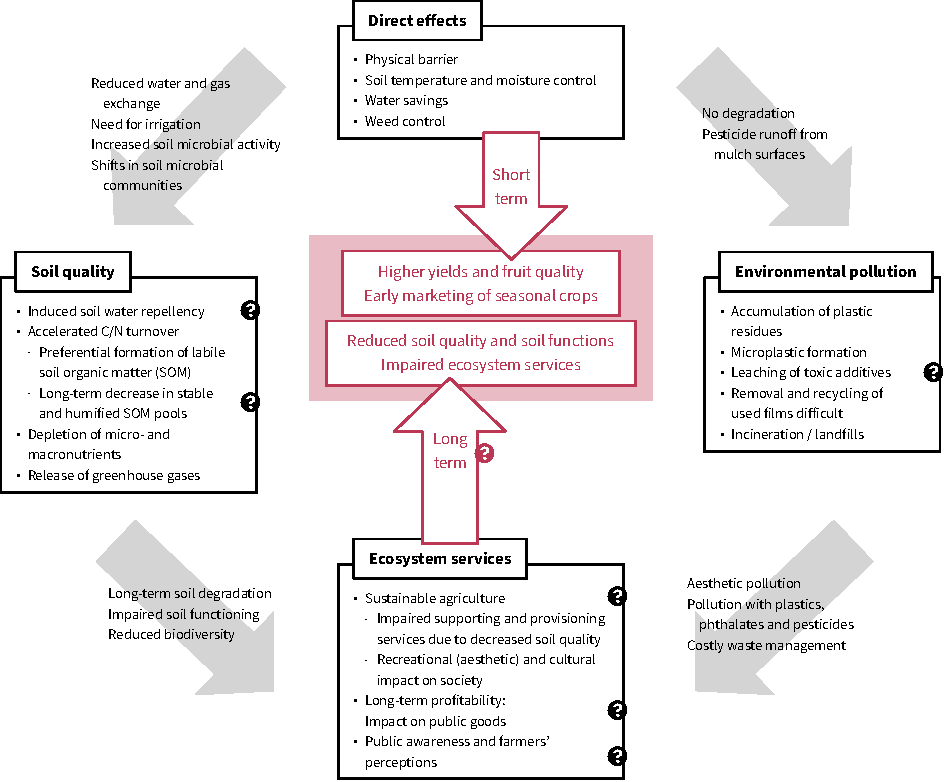
\includegraphics[width=\textwidth]{figures/mulching-overview}
	\caption[Schematic representation of the impacts of plastic mulch use on soil quality, pollution, and implications on agronomy and ecosystem services.]{Schematic representation of the impacts of plastic mulch use on soil quality, pollution, and implications on agronomy and ecosystem services; question marks indicate need for research.}
	\label{fig:mulching-overview}
	\forcerectofloat
\end{figure*}

\section{Conclusions}
\label{sec:plastic-mulching:conclusions}

This literature review identified certain reasons for farmers to apply plastic mulches in agriculture, but it also identified a number of risks and less beneficial effects of plastic mulching with regard to waste treatment, life cycle balance, and impact on soil quality. This includes the persistence of unrecovered plastic mulch in soil, their potential to alter soil quality by shifting the edaphic biocoenosis, accelerating carbon and nitrogen metabolism, as well as potentially degrading \ac{som}. This further includes inducing soil water repellency, increasing the risk of mycotoxin formation in soil and an enhanced release of climate relevant gases. Although several attempts have been made to extend the life cycle of plastic mulches and to reduce their input to soil by recovering and recycling used mulching films, in some cases the cost and effort of these options seem to outweigh their benefits from yield increases, water savings, and facilitated pest control. If, in addition, external effects of mulching on (public) goods or resources like soil quality, biodiversity, or recreation are taken into account, a holistic ecosystem services assessment could make plastic mulching uneconomic and unsustainable.

Comprehensive research with the aim of gaining an extensive understanding of the processes governing the impacts of mulching on soil quality is needed. As most of these biogeochemical processes are not yet sufficiently understood, a final judgment on the implications of plastic mulching for the environment will require long\-/term field experiments combined with targeted process\-/orientated studies on a laboratory scale in order to be able to estimate and potentially avoid environmental risks such as soil degradation. This process understanding is of particular importance for the development of truly biodegradable mulches. In order to assess the contribution of plastic mulching to the pollution with plastic debris and to changes in \ac{som} composition and quality, future research should focus on more detailed soil characterization techniques such as \ac{py-gc-ms} or thermogravimetric approaches as a basis for further impact assessments and life cycle analyses. Similarly, analytical methods which can detect, identify, and quantify plastic debris in soil, need to be developed.

The currently rather unquestioned application of plastic mulching may be attributed to the lack of long\-/term studies and attention in the mass media addressing the potential risks for the soil, biota, and society. Future research should analyze why and under which premises plastic mulching is accepted by farmers, the public, and further stakeholders of the agronomic sector and which long\-/term incentives drive farmers to apply plastic mulches. Deeper knowledge of these aspects would help to make both the agribusiness and society more environment\-/friendly.

% !TeX spellcheck = en_US

\chapter{Quantitative Analysis of PET Plastic Debris in Soil via TGA/MS}
\label{ch:tga-ms-method}

\paragraph{Abstract} The use of plastic materials in daily life\marginnote{This chapter is based on: \fullcite{DavidQuantitative2018}.\par See \nameref{ch:author-contributions}, page~\pageref{ch:author-contributions}, for details.}, industry, and agriculture can cause soil pollution with plastic debris down to the micrometer range, namely, microplastics.
The quantitative assessment of plastic debris in soil has been limited so far. Until now, microplastic analyses in soil require laborious sample cleanup and are mostly restricted to qualitative assessments. In this study, we applied \ac{tga-ms} to develop a method for the direct quantitative analysis of \ac{pet} without further sample preparation.
For this, soil samples containing \SI{1.6(2)}{\percent} \ac{Corg} were spiked at \SIrange{2.3}{45.9}{\gram\per\kilo\gram} \ac{pet} plastic debris from recycled bottles. \textsc{dl}-Cysteine was used as an internal standard. Sample mixtures were pyrolyzed with a \SI{5}{\kelvin\per\minute} ramp (\SIrange{40}{1000}{\degreeCelsius}), while sample mass loss and \ac{ms} signal intensities of typical \ac{pet} pyrolysis products were recorded.
We found signal intensities linearly responding to \ac{pet} concentrations. The most promising results were obtained with the internal standard-corrected \ac{pet} pyrolysis product vinylbenzene\slash benzoic acid (\SI{105}{\mz}, adj. $R^2$ = \num{0.987}). The \acp{lod} and \acp{loq} were \SIlist{0.7;17.2}{\gram\per\kilo\gram} \ac{pet}, respectively.
Our results suggest that \ac{tga-ms} can be an easy and viable complement to existing methods such as \ac{ted-gc-ms} or microspectroscopic techniques.

\section{Introduction}

Microplastics are synthetic polymers with typical particle sizes smaller than \SI{5}{\milli\meter} either disintegrated from larger plastic parts or originally produced in particulate form \citep{CincinelliMicroplastic2017}.
Microplastics have been recently recognized as a ubiquitous environmental contaminant in marine and fresh waters, sediments, and organisms \citep{KarlssonScreening2017,RochmanMicroplastics2018}. However, the sources, pathways, and reservoirs of microplastics in terrestrial systems are still hardly known \citep{DrisSynthetic2016}.

Microplastics could be introduced into soil via
\begin{enumerate*}
	\item air transport of non-managed plastic wastes, littering, and street runoff \citep{DrisSynthetic2016,BlasingPlastics2018},
	\item disintegration of agriculture plastics such as mulch films, tarpaulins, tunnels, and pipes \citep{LambertOccurrence2014}, or
	\item application of sewage sludge and reclaimed wastewater containing plastic microbeads or
	fibers \citep{BlasingPlastics2018,ZubrisSynthetic2005}.
\end{enumerate*}
In this respect, the presence of plastic fragments has become an important parameter to describe urban soils and Technosols \citep{RilligMicroplastic2012,NizzettoAre2016}. Particularly in transitional and developing economies, used agricultural plastic mulches and other plastic wastes may be incorporated into the soil of agricultural fields \citep{DuisMicroplastics2016} and household gardens \citep{vanderWalHuertos2011}, where they are likely to become an environmental issue \citep{SintimBiodegradable2017}. Plastic debris is assumed to further accumulate in the soil food web \citep{RilligMicroplastic2012}, to function as sorbent for agrochemicals \citep{RamosPolyethylene2015}, or adversely affect soil organisms \citep{KirsteinDangerous2016}, eventually decreasing soil stability and quality.
Synthetic polyester fibers, namely \ac{pet}, as used in this screening study, have already been found in sewage sludge \citep{ZubrisSynthetic2005} and are continuously introduced into the environment by washing and wearing synthetic textiles \citep{PircEmissions2016}. Agricultural tarpaulins or discarded \ac{pet} bottles are another source of plastic pollution in soil.

In order to assess the content of plastic debris in agricultural soil and adjacent freshwater sediments, analytical assays for the identification and quantification of plastic debris in complex environmental matrices are needed \citep{BlasingPlastics2018}. Microscopic techniques, mainly light microscopy, are currently the most used but pose extraordinarily high requirements on laboratory cleanliness and typically require labor-intensive preconcentration procedures \citep{WoodallUsing2015}. If these requirements are not
met, misinterpretation coming from false positive results is likely \citep{LachenmeierMicroplastic2015}. Microspectroscopic techniques, such as \ac{ftir} spectroscopy with optional \ac{atr} or Raman microspectrometry, represent alternative approaches. The latter may help to fulfill the analytical requirements of distinguishing particles or fibers of synthetic origin from natural matrix structures such as cellulose fibers or silicate particles. \citet{PrimpkeAutomated2017} presented an interesting method for the automated detection of plastic debris on membrane filters using advanced image analysis software. Such techniques have been used for more easily accessible and homogeneous atmospheric or aqueous matrices so far but not for soil \citep{IoakeimidisDegradation2016,FischerIdentification2015,Comnea-StancuIdentification2016}, and they often produce only qualitative results \citep{BlasingPlastics2018} because of interferences from \ac{som} autofluorescence.

Another promising technique may be alkali depolymerization of \ac{pet} and subsequent analysis of depolymerized building blocks bisphenol A and \textit{p}-phthalic acid in sludge, sediments, and mussels via \ac{lc-ms} \citep{WangSimple2017}. However, both bisphenol A and \textit{p}-phthalic acid are not specific for the analysis of one single polymer, extraction from soil may be incomplete, and leaching and mobilization of building block compounds from the polymer backbone into the environment may produce ambiguous results \citep{WangSimple2017}. \citet{ElertComparison2017} achieved recovery rates of about \SI{80}{\percent} \ac{pet} extracted from soil with hexafluoroisopropanol followed by \ac{sec} and reverse-phase \ac{lc}.

In contrast, analytical techniques based on sample pyrolysis have the potential to overcome the aforementioned drawbacks of microscopic and extraction methods in terms of higher specificity, lower sample preparation efforts, and facilitation of semiquantitative to quantitative analyses.
For example, by using Curie point \ac{py-gc-ms}, \ac{pet} quantification in fish required less than \SI{5}{\micro\gram} of substance when combined with prior enzymatic and chemical digestion \citep{FischerSimultaneous2017}.
However, high sand contents made an additional density separation step necessary, which is challenging considering the high density of \ac{pet}. Here, \citet{DumichenAnalysis2015} were the first to successfully apply and validate a quantitative method for \ac{pe} in soil.
The authors established a two-step procedure involving pyrolysis of \ac{pe}-spiked soil via \ac{tga} and capturing of pyrolysis gases followed by \ac{ted-gc-ms}. The same method has also been applied for the determination of \ac{pet}, so far only with qualitative results \citep{DumichenFast2017}.

An alternative to this two-step approach is on-line \ac{tga-ms}, measuring simultaneously the masses of gases evolving during thermal treatment. Thermal treatment can either be oxidation (combustion) or pyrolysis in an inert \ch{Ar} atmosphere. A defined portion of gaseous degradation products are transferred into a quadrupole \ac{ms} via a heated capillary or a capillary\-/less orifice. The mass loss at a specific temperature is then related to the \ac{ms} signal of gaseous pyrolysis products.
Even without chromatographic separation, analytes with the same or similar pyrolysis products as the matrix may be distinguished from each other\sidenote{For instance plastic pyrolysis products from soil pyrolysis products.} according to their distinct decomposition temperatures.

So far, \ac{tga-ms} has been successfully applied for characterizing combustion or pyrolysis products of soils \citep{PallasserSoil2013,EdmondsonBlack2015,TamimiFate2017}, sediments \citep{FindorakovaAssessment2017}, and polymers \citep{PagaczThermal2015,SchindlerNovel2013}. However, complex mixtures of plastic debris and soil have not yet been assessed.
With this proof\-/of\-/principle work, we aimed to evaluate the potential of a capillary \ac{tga-ms} system to qualitatively and quantitatively determine \ac{pet} in a spiked soil without any preseparation of \ac{pet} plastic debris from soil.
We focused on the determination and quantification of characteristic pyrolysis products of \ac{pet} such as benzoic acid and vinyl and alkylbenzenes (\SI{105}{\mz} fragment) and biphenyl (\SI{154}{\mz} fragment) \citep{DumichenFast2017,DimitrovAnalysis2013,DuemichenAssessment2014}; the latter being formed by a radical reaction and intramolecular ring formation \citep{RichterFormation2000,KawaiCharacterization2008}.
The formation of these pyrolysis products can then be related to their specific degradation temperatures as determined by \ac{tga}. \textsc{dl}-Cysteine was used as internal standard for normalizing the present detector signal and ionization state.
By using a capillary \ac{tga-ms}, we wanted to provide an easy-to-use instrumental setup for plastic analysis. Since some studies have discussed the potential of the \ac{tga-ms} capillary to become blocked during polymer measurements \citep{SchindlerNovel2013,DuemichenAssessment2014}, particular attention was paid to monitoring and maintaining a working capillary throughout all our experiments.
In this work, we study the possibilities of using the capillary \ac{tga-ms} device for a quicker and cheaper assessment of plastic debris in soil within the soil matrix and the influences of \ac{som} on the detection limits.

\section{Experimental}

\subsection{Materials}

Cryomilled \ac{pet} dust obtained from mechanical shredding of bottle recyclate\sidenote{PETKA CZ, Brno, Czech Republic.} (\SIrange{0.15}{0.4}{\milli\meter} dominant particle size) was used as the microplastic sample. \Iac{pet} standard\sidenote{\cas{25038-59-9}, PlasticsEurope, Frankfurt, Germany.} and \iac{pet} water bottle sample\sidenote{EDEKA, Hamburg, Germany.} were used to assess \ac{pet} dust quality.
For the preparation of calibration series, a standard loamy sand (\SI{75}{\percent} sand, \SI{16}{\percent} silt, \SI{9}{\percent} clay)\sidenote{LUFA 2.2, \foreignlanguage{ngerman}{Landwirtschaftliche Unter\-suchungs- und Forschungsanstalt}, Speyer, Germany.} with \SI{1.6(2)}{\percent} \ac{Corg} content was used. \textsc{dl}-Cysteine\sidenote{\cas{3374-22-9}, \SI{98}{\percent} purity, Carl Roth, Karlsruhe, Germany.} served as the internal standard for \ac{tga-ms} pyrolysis measurements.

\subsection{Quality Assessment of the \Acs{pet} Dust}

In order to compare the potential difference in the physicochemical properties of the shredded microplastic sample and the \ac{pet} standard, \ac{dsc}\sidenote{Q1000, TA Instruments, New Castle, USA.} was used to determine their melting temperature and melting enthalpy.
The thermal history of \ac{pet} samples was erased with a preheating run from \SIrange[range-phrase = { to }]{40}{310}{\degreeCelsius} followed by a cooling run from \SIrange[range-phrase = { to }]{310}{-20}{\degreeCelsius}.
For the subsequent measurement, the heating run was repeated from \SIrange[range-phrase = { to }]{-20}{310}{\degreeCelsius}. All runs were performed in hermetically sealed pans\sidenote{TZero, TA Instruments, New Castle, USA.} under a \SI{50}{\milli\liter\per\minute} \ch{N2} flow and a thermal ramp of \SI{+-10}{\kelvin\per\minute}. All \ac{dsc} analyses were performed in triplicate.

\subsection{Preparation of Spiked Soil Samples}

Two calibration series were prepared, each in duplicate. For both experiments, a microscale\sidenote{Sartorius SE 02-OCE, Göttingen, Germany.} and \SI{85}{\micro\liter} alumina \ac{tga} crucibles\sidenote{Netzsch, Selb, Germany.\label{sn:netzsch}} were used. All specimens were weighed directly into the \ac{tga} crucible and carefully mixed.

The first calibration series was performed without internal standard. To this end, between \SIrange[range-phrase = { and }]{42.98}{50.79}{\milli\gram} of soil was spiked with \SIrange{0.28}{2.02}{\milli\gram} of milled \ac{pet} bottle recyclate in order to prepare five different \ac{pet} concentrations in soil ranging from \SIrange{5.6}{41.8}{\gram\per\kilo\gram}.
For the second calibration series, about \SI{1}{\percent} of \textsc{dl}-cysteine (\SIrange{0.87}{1.08}{\percent}; \SIrange{0.41}{0.52}{\milli\gram}) was added as internal standard to \ac{pet}-spiked and blank soil.
Here, seven different concentrations were prepared ranging from \SIrange[range-phrase = { to }]{2.3}{45.9}{\gram\per\kilo\gram} \ac{pet} (\SIrange{0.10}{2.24}{\milli\gram} added to \SIrange{44.18}{46.83}{\milli\gram} of soil).

\textsc{dl}-Cysteine has not been used in \ac{tga-ms} as internal standard yet. In this work, it was selected to obtain an easily detectable and distinguishable pyrolysis product with lower molecular weight than the observed \ac{pet} pyrolysis products. The amount of \ch{S} in \ac{som} is approximately two orders of magnitude lower than that in \textsc{dl}-cysteine \citep{BlumeScheffer2016}. Pyrolysis of \textsc{dl}-cysteine provides a strong signal at \SI{33}{\mz} corresponding to the \ch{SH-} ion \citep{ChoiDetermination1995}, which was proven absent both in \ac{pet} and \ac{som} pyrolysis products, in a relatively narrow pyrolysis temperature range (Appendix, Figure~\ref{fig:cysteine-comparison}).
Normalization of analyte signals to the signal of the internal standard is of considerable importance to obtain more stable peak responses during routine \ac{tga-ms} measurements. Particularly during long measurement series of various samples, non-standardized \ac{ms} signals may vary with respect to current ionization and detector state \citep{NetzschGeratebauMS2010}.

\subsection{\Acs{tga-ms} Analysis}\label{sec:tga-ms-analysis}

All samples were subjected to a \SI{5}{\kelvin\per\minute} pyrolysis ramp from \SIrange[range-phrase = { to }]{40}{1000}{\degreeCelsius} under a \SI{20}{\milli\liter\per\minute} \ch{Ar} 5.0 gas flow in a \num{2}-fold evacuated \ch{Ar}-filled \ac{tga} chamber\sidenote{STA 449 F3 Jupiter TGA analyzer, Netzsch, Selb, Germany.}. The \ac{tga} was coupled with a QMS 403 C Aëolos \ac{ei} quadrupole \ac{ms}\sideref{sn:netzsch} via a \SI{2.2}{\meter} long, \SI{75}{\micro\meter} wide, untreated fused silica capillary\sidenote{SGE Analytical Science, Ringwood, Victoria, Australia.} heated to \SI{300}{\degreeCelsius}.
The mass resolution as contribution to neighboring masses of \num{40}/\num{41} was \SI{<50}{ppm}. The detector was set to on-line mode in order to directly detect preselected \si{\mz} ratios from \numrange[range-phrase = { to }]{12}{154}.
Dependent on the \si{\mz} ratios of interest, the following settings were used: For \si{\mz} ratios of \numrange{12}{32} and \num{44}, the \ac{sem} was adjusted to \SI{1400}{\volt}, a dwell time of \SI{1}{\second}, and a resolution of \SI{50}{au}. For \si{\mz} \numrange{33}{154}, \iac{sem} voltage of \SI{2400}{\volt}, a dwell time of \SI{5}{\second}, and a resolution of \SI{250}{au} were applied.
Both calibration series, with and without \textsc{dl}-cysteine as internal standard, were measured together with six blank soil samples.

\Acp{lod} and \acp{loq} [\si{\micro\gram\per\milli\liter}] were calculated using Equations~\ref{eq:lod} and \ref{eq:loq}, respectively, in accordance with the German standard \citet{DIN32645Chemical2008} as implemented in the R package ``envalysis''\sidenote{The package source is available at \doi{10.5281/zenodo.1240305}.} (version 0.3.3).

\begin{equation}
\mathrm{LOD} = \frac{\sigma_\mathrm{blank}}{a} \cdot t_{n-1;0.01} \sqrt{n^{-1} + m^{-1}}
\label{eq:lod}
\end{equation}

\begin{equation}
\mathrm{LOQ} = k \cdot \frac{\sigma_{xy}}{a} \cdot t_{n-2;0.01} \sqrt{n^{-1} + m^{-1} + \frac{(\mathrm{LOQ}-\overline{x})^2} {S_{xx}}}
\label{eq:loq}
\end{equation}

Therein, $\sigma_\mathrm{blank}$ is the \ac{sd} of integrated peak areas from blank measurements, $\sigma_{xy}$ is the residual \ac{sd}, and $a$ [\si{\milli\liter\per\micro\gram}] is the slope of the calibration curve. $t$ is the \SI{99}{\percent} percentile of the Student's $t$ distribution with $n - 1$ and $n - 2$ degrees of freedom, $n$ as the total number of measurements, and $m$ as the number of replicates. $k = 3$ is the recommended certainty factor for the \ac{loq}; $\overline{x}$ is the arithmetic mean of all standard concentrations, and $S_{xx}$ [\si{\square\micro\gram\per\square\milli\liter}] is the sum of squares of $x$. Note that calculating the \ac{loq} is an iterative process with $\mathrm{LOQ} = k \cdot \mathrm{LOD}$ as initial value.

\subsection{Transfer Capillary Control Experiments}

Although some authors use \ac{tga-ms} for pyrolysis of polymers without reporting problems \citep{PagaczThermal2015}, it has been discussed whether the heated capillary used for the transfer of the pyrolysis product from the \ac{tga} chamber to the \ac{ms} detector may become blocked by condensing pyrolysis products during measurements \citep{SchindlerNovel2013,DuemichenAssessment2014}.
In order to control the state of the transfer capillary, the following control experiments were conducted: after each spiked sample, a cleaning run with an empty crucible and a \SI{10}{\kelvin\per\minute} heating ramp from \SIrange[range-phrase = { to }]{40}{1000}{\degreeCelsius} in a \SI{50}{\milli\liter\per\minute} synthetic air flow was followed by pyrolysis\sidenote{Under the same conditions as spiked samples.} of calcium oxalate hydrate (\ch{CaC2O4 * H2O})\sidenote{\cas{5794-28-5}, Sigma-Aldrich, Steinheim, Germany.}.
Constant \ac{ms} signals of calcium oxalate pyrolysis products ensured a consistently working capillary. Signals of \SI{105}{\mz} from cleaning runs and oxalate pyrolysis events were averaged and taken as the noise throughout the complete temperature range in order to assess a potential residual signal carried over from the capillary and originating from impurities remaining in the transfer capillary during spiked sample measurements and potential leaks during control experiments.

For the least concentrated \ac{pet} sample, the \ac{snr} (Equation~\ref{eq:snr}) was calculated on the basis of the mean \si{\mz} signal $\mu_\text{sample}$ over a temperature range of \SIrange{300}{650}{\degreeCelsius} divided by the \ac{sd} of a cleaning run ($\sigma_\text{clean}$) containing either no sample or oxalate \citep{WellsSignal2011}.

\begin{equation}
\mathrm{SNR} = \frac{\mu_\text{sample,300--650\,°C}}{\sigma_\text{clean, 40--1000\,°C}}
\label{eq:snr}
\end{equation}

In addition, the capillary pressure was controlled before every measuring sequence to monitor constant throughput.

\section{Results and Discussion}

\subsection{Quality Assessment of the \Acs{pet} Recyclate}

The \ac{dsc} measurements revealed a comparable melting temperature ($T_m$) and specific enthalpy of fusion ($\Delta H^\circ_\text{fus}$) for
the \ac{pet} recyclate ($T_m$ = \SI{243.6(4)}{\degreeCelsius}, $\Delta H^\circ_\text{fus}$ = \SI{48(3)}{\joule\per\gram}),
the PET standard ($T_m$ = \SI{243.1(1)}{\degreeCelsius}, $\Delta H^\circ_\text{fus}$ = \SI{48(3)}{\joule\per\gram}), and
the \ac{pet} water bottle obtained from a common German retail chain store ($T_m$ = \SI{246.5(2)}{\degreeCelsius}, $\Delta H^\circ_\text{fus}$ = \SI{50(6)}{\joule\per\gram}; averaged heat flows are given in Figure~\ref{fig:dsc}).
Therefore, the \ac{pet} recyclate was deemed qualitatively representative for further method development.

\subsection[\Acs{tga-ms} Results of \Acs{pet}-Spiked Soils]{\Acs{tga-ms} Results of \Acs{pet}-Spiked Soils with and without Internal Standard}

\begin{marginfigure}
	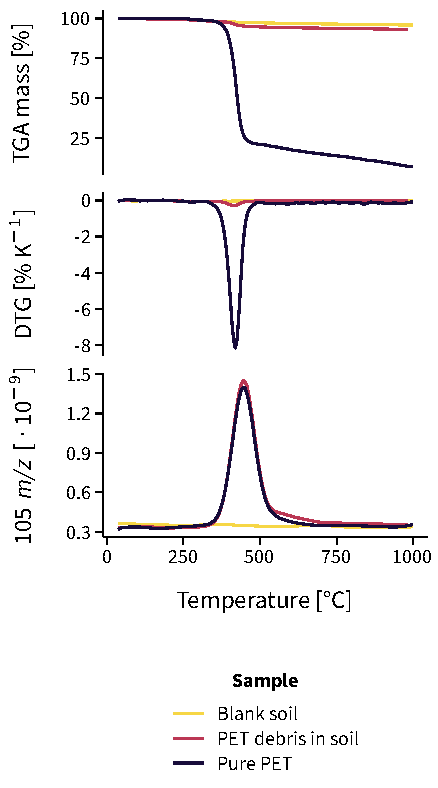
\includegraphics[width=\marginparwidth]{figures/tga-dtg-sample}
	\caption[\Ac{tga} and \ac{dtg} curves of blank soil, pure \ac{pet}, and an exemplary mixture of \ac{pet} debris in soil.]{\Ac{tga} and \ac{dtg} curves and normalized \SI{105}{\mz} ratios of blank soil, pure \ac{pet} (\SI{1.73}{\milli\gram}), and an exemplary mixture of \SI{37.1}{\gram\per\kilo\gram} \ac{pet} debris (\SI{1.74}{\milli\gram}) in soil.}
	\label{fig:tga-dtg-sample}
\end{marginfigure}

The degradation onsets of \ac{pet}, blank soil, and the internal standard \textsc{dl}-cysteine were \SIlist{382;208;205}{\degreeCelsius}, respectively. Figure~\ref{fig:tga-dtg-sample} shows the \ac{tga} curves, \acf{dtg} curves, and \SI{105}{\mz} ratios of blank soil, pure \ac{pet}, plastic dust, and an exemplary \SI{37.1}{\gram\per\kilo\gram} \ac{pet} mixture with soil. The \ac{tga} curve of soil indicated a mass loss of \SI{0.27(3)}{\percent} between \SIrange[range-phrase = { and }]{40}{150}{\degreeCelsius} typically ascribed to soil residual humidity.
Above \SI{208}{\degreeCelsius}, degradation of \ac{som} caused a mass loss of \SI{1.5(1)}{\percent} (calculated until \SI{380}{\degreeCelsius}). The pure \ac{pet} degraded between \SIrange[range-phrase = { and }]{380}{650}{\degreeCelsius} as indicated by a considerable mass loss and accompanied by a peak for \SI{105}{\mz}.
Such a peak was absent in blank soil without any \ac{pet}. As for pure \ac{pet}, soil samples spiked with microplastic \ac{pet} lost its residual humidity between \SIrange[range-phrase = { and }]{40}{150}{\degreeCelsius}.
\Ac{som} degraded above \SI{208}{\degreeCelsius}. The mass loss between \SIrange[range-phrase = { and }]{382}{650}{\degreeCelsius} was attributed to the degradation of \ac{pet}. \textsc{dl}-Cysteine added as internal standard rapidly degraded between \SIrange[range-phrase = { and }]{205}{250}{\degreeCelsius} (Figures~\ref{fig:tga-ms} and \ref{fig:cysteine-tests}).

\begin{figure*}
	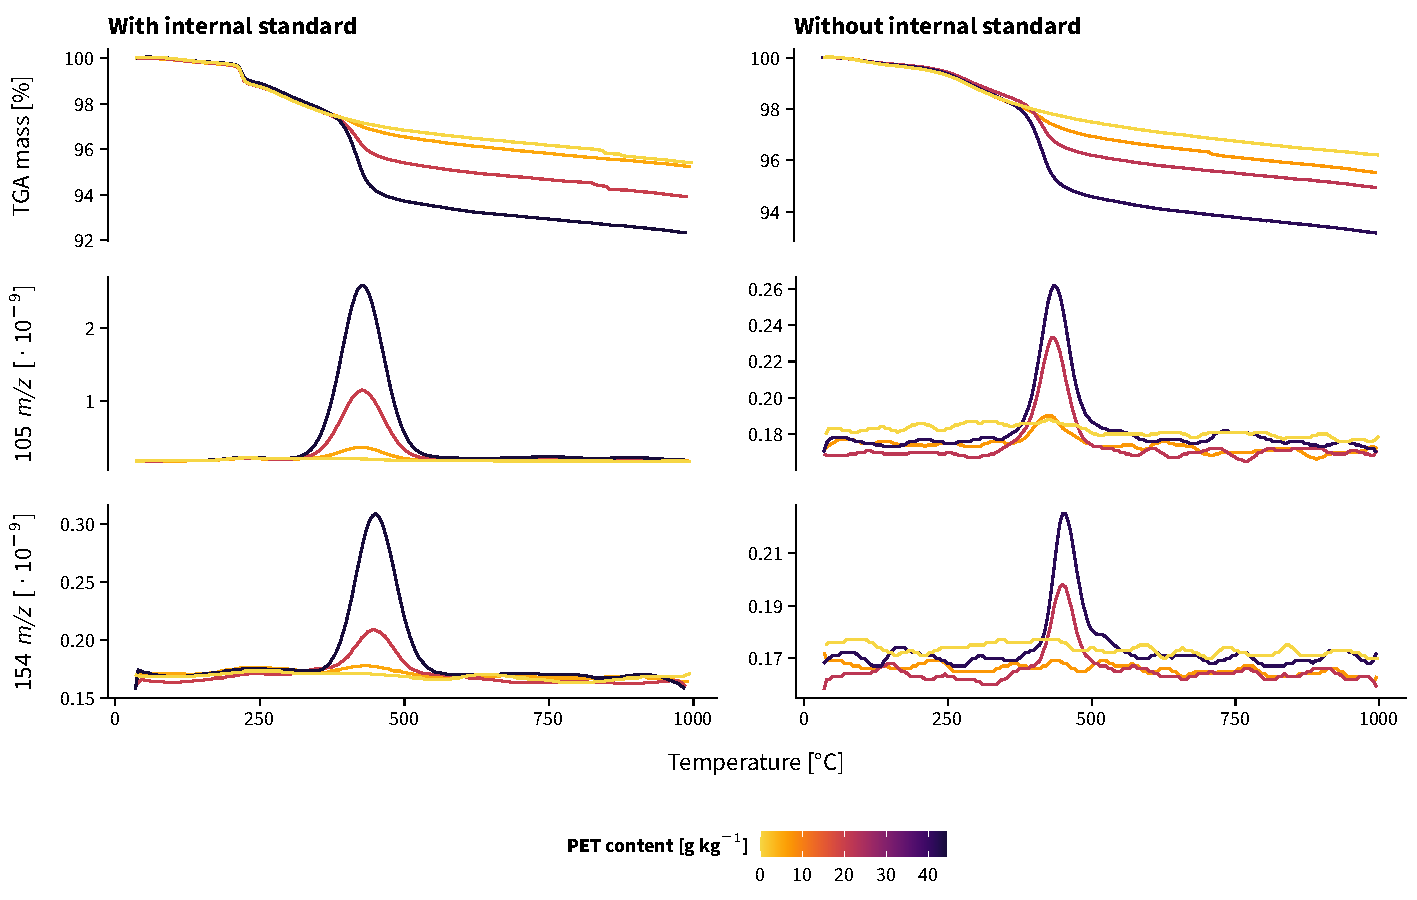
\includegraphics[width=\textwidth]{figures/tga-ms}
	\caption[Exemplary \ac{tga-ms} curves of soil spiked at three different \ac{pet} contents with or without internal standard.]{Exemplary \ac{tga-ms} curves (mass loss, together with \SIlist{105;154}{\mz} ratios) of soil spiked at three different \ac{pet} contents either with or without \textsc{dl}-cysteine as internal standard.}
	\label{fig:tga-ms}
	\forcerectofloat
\end{figure*}

Irrespective of the internal standard, the \SIlist{105;154}{\mz} fragments evolving from pyrolysis of \ac{pet} in soil (Figure~\ref{fig:tga-ms}) corresponded to the mass loss of \ac{pet} on the \ac{tga} curves.
Although these signals have been reported as the most intensive signals occurring during \ac{pet} thermal degradation \citep{DumichenFast2017,DimitrovAnalysis2013}, they cannot be considered absolutely specific for \ac{pet} in soil.
To a certain extent, \SIlist{105;154}{\mz} are also produced during the pyrolysis of \ac{som} \citep{SchultenThermal1999} and other polymers that contain phthalate plasticizers. However, relating \ac{ms} signals to the specific temperature range of \ac{pet} degradation, namely \SIrange{300}{650}{\degreeCelsius}, enabled us to reduce the false positive detection of \ac{pet} degradation products and to correlate them with the nominal \ac{pet} content in soil.
It remains noteworthy that this approach may be restricted to our given setup. Interferences may occur when analyzing other soils containing complex mixtures of different polymers.

Apart from \ac{pet} and \ac{som} degradation products, the sharp mass loss at \SIrange{205}{250}{\degreeCelsius} corresponded to the degradation of \textsc{dl}-cysteine added as internal standard (\SI{33}{\mz}). \textsc{dl}-Cysteine signal intensities were linear in the anticipated concentration range of \SIrange{0.25}{1.78}{\percent} in soil (Figures~\ref{fig:tga-ms} and \ref{fig:cysteine-tests}).

Peaks of \SIlist{105;154}{\mz} ratios integrated within \SIrange{300}{650}{\degreeCelsius} were used for linear calibration curves of \ac{pet} pyrolysis products (Figure~\ref{fig:tga-calibration}). Corresponding \acp{lod}, \acp{loq}, adj. $R^2$s, and \acp{rse} are presented in Table~\ref{tab:tga-calibration}.
Within a linear range of \SIrange{2.5}{40}{\gram\per\kilo\gram} \ac{pet}, the best goodness\-/of\-/fit measures, these were an adj. $R^2$ of \num{0.987} and \iac{rse} of \SI{3.21}{\percent}, were achieved with the \SI{105}{\mz} signal after internal standard addition.
The \ac{lod} and \ac{loq} were \SIlist{0.7;17.2}{\gram\per\kilo\gram} \ac{pet}, respectively. For internal standard-corrected \SI{154}{\mz}, the \ac{lod} was comparable to that of \SI{105}{\mz} as a result of a low background noise.
However, the \ac{ms} signal responded less linearly with increasing \ac{pet} concentrations. Without internal standard, the curve linearity, \acp{lod}, and \acp{loq} were considerably worse.

\begin{figure*}
	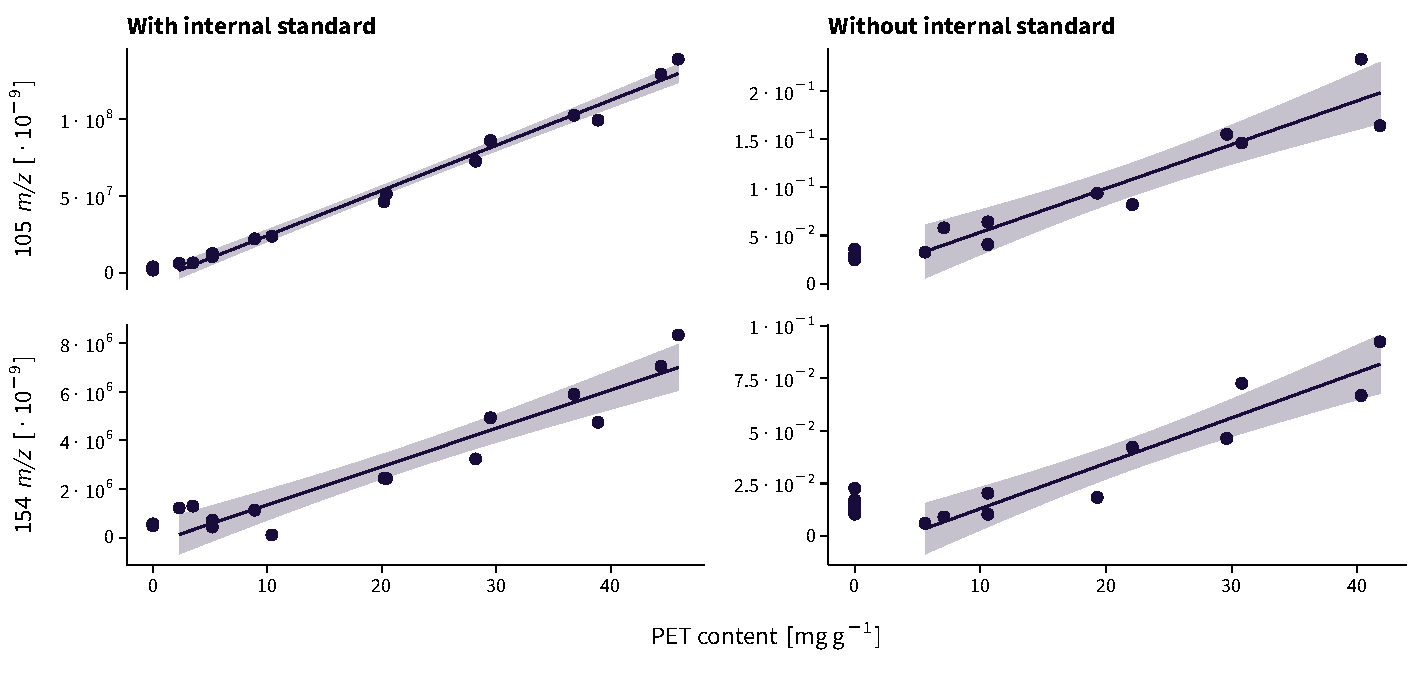
\includegraphics[width=\textwidth]{figures/tga-calibration}
	\caption[\Ac{tga-ms} calibration curves of \ac{pet} in soil.]{\Ac{tga-ms} calibration curves of \ac{pet} (\SIlist{105;154}{\mz}) in soil normalized to the sample mass when no internal standard was added or normalized to \SI{33}{\mz} from the pyrolysis of \textsc{dl}-cysteine as internal standard; shaded bands represent the \SI{95}{\percent} \acs{ci} of the linear model;  calibration parameters are summarized in Table~\protect\ref{tab:tga-calibration}.}
	\label{fig:tga-calibration}
	\forceversofloat
\end{figure*}

\begin{table}[b]
	\centering\footnotesize
	\caption[\Ac{tga-ms} calibration parameters.]{\Ac{tga-ms} calibration parameters; see Figure~\protect\ref{fig:tga-calibration} for calibration curves.}\label{tab:tga-calibration}
	\begin{tabular}{llS[table-format = 1.3]S[table-format = 2.2]S[table-format = 2.1]S[table-format = 3.1]}
		\toprule
		{\si{\mz}} & {Internal standard} & {adj. $R^2$} & {\Acs{rse} [\si{\percent}]} & {\Acs{lod} [\si{\gram\per\kilo\gram}]} & {\Acs{loq} [\si{\gram\per\kilo\gram}]} \\
		\midrule
		105 & no & 0.870 & 12.76 & 2.5 & 510.0 \\
154 & no & 0.888 & 11.75 & 5.8 & 184.0 \\
105 & yes & 0.987 & 3.21 & 0.7 & 17.2 \\
154 & yes & 0.893 & 9.57 & 0.6 & 65.3 \\
		\bottomrule
		\multicolumn{6}{p{.72\textwidth}}{\acs{rse} = \acl{rse} of the slope estimate.} \\
	\end{tabular}
\end{table}

In contrast to our study, \citet{DumichenFast2017} used a common \ac{pe} bag shredded to microplastic particles and an uncharacterized sandy topsoil sampled from an urban area. The authors analyzed various $n$-alkadienes as characteristic products of \ac{pe} pyrolysis via \ac{ted-gc-ms}. They spiked the soil with \SIrange[range-phrase = { to }]{15}{150}{\gram\per\kilo\gram} \ac{pe} concentrations and achieved linear calibration curves of integrated \SI{55}{\mz} signals as a characteristic fragment for eight different $n$-alkadienes with an adj. $R^2$ ranging from \num{0.5395} for 1,11-dodecadiene to \num{0.9958} for 1,15-hexadecadiene. Their highest signal response was observed for 1,13-tetradecadiene, for which an adj. $R^2$ = \num{0.9884} and \iac{loq} of \SI{10}{\gram\per\kilo\gram} \ac{pe} were determined.
\Acp{rse} of slope estimates inferred from the calibration curves by \citet{DumichenAnalysis2015} varied from \SIrange[range-phrase = { to }]{2.97}{12.41}{\percent}. In this respect, our \ac{loq}, adj. $R^2$, and \ac{rse} obtained from \SI{105}{\mz} after internal standard correction (\SI{17.2}{\gram\per\kilo\gram} \ac{pet}) were generally comparable with those by \citet{DumichenAnalysis2015}.
Small differences in adj. $R^2$s, \acp{lod}, and \acp{loq} are probably due to use of a different soil and polymer. In addition to that, we tried to mimic a potential environmentally relevant \ac{pet} sample with the dust that originated from shredding of recycled \ac{pet} bottles.
Although checked by \ac{dsc}, recycled \ac{pet} dust may contain impurities from different polymer or paper microparticles.
When pyrolyzed, such impurities may interfere with \num{105} or \SI{154}{\mz} signals produced by pure \ac{pet}.
Together with \ac{pet} concentrations up to \num{6} times lower than the \ac{pe} contents used by \citet{DumichenAnalysis2015}, a slightly higher variation in detector responses and, with that, a reduced goodness of fit of the calibration curves are deemed plausible. One option to further reduce detector variation could be to recalibrate the \ac{sem} voltage after every sample run, which is however, not practical for routine analyses. This is why we normalized the obtained signals to an internal standard, which increased the linearity of the calibration curves (Figure~\ref{fig:tga-calibration}).
Moreover, \ac{tga-ms} has so far mostly been used to analyze pure chemicals with known stoichiometry of decomposition reactions and low-molecular-weight pyrolysis products \citep{HotovaQuantitative2016}. Reactions of pyrolysis products potentially occurring in the heated capillary may therefore be another reason for less sensitive signal responses, which we assessed with regular capillary tests.

\subsection{Transfer Capillary Control Experiments}

Series of cleaning runs confirmed that no signal of \SI{105}{\mz}\sidenote{As the stronger of the \si{\mz} ratios analyzed.} was detected in runs following soil analysis. Figure~\ref{fig:tga-capillary-checks} shows worst case scenarios, this is cleaning run and oxalate run after the most concentrated spiked samples, where the probability of capillary blocking was the highest, both with and without \textsc{dl}-cysteine as internal standard.
The results are in comparison with the best case scenarios, namely cleaning run and oxalate run after the least concentrated spiked samples and the \SI{105}{\mz} signals of both least concentrated \ac{pet} samples.
Note that the baselines of the least spiked samples (\SI{2}{\gram\per\kilo\gram} \ac{pet}) vary in comparison to cleaning runs, because the cleaning runs were performed in synthetic air.

\begin{figure*}
	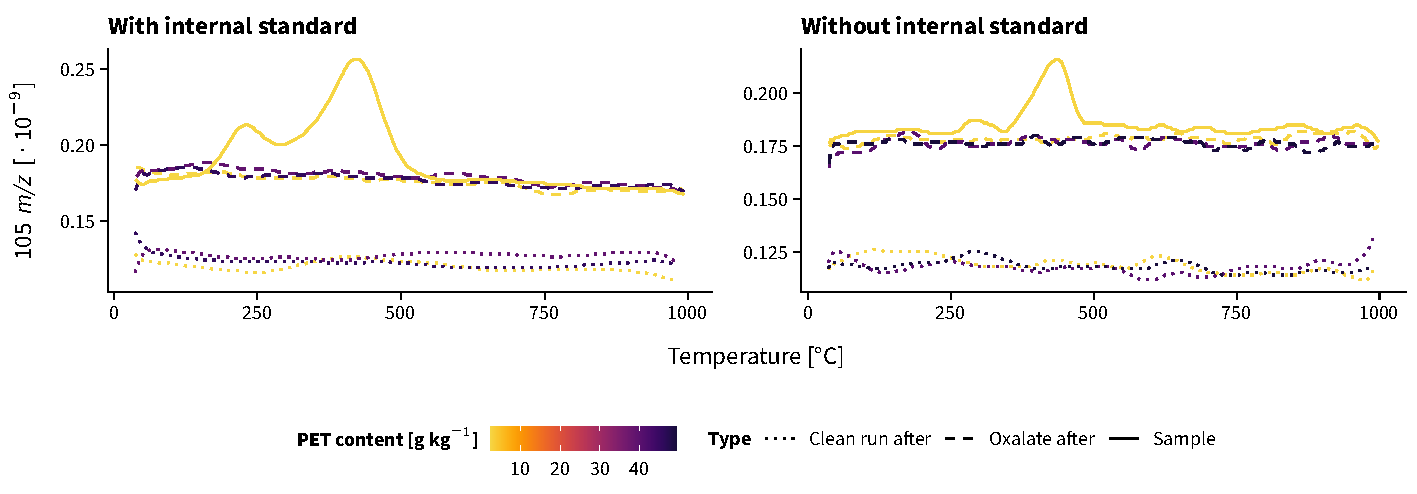
\includegraphics[width=\textwidth]{figures/tga-capillary-checks}
	\caption[\SI{105}{\mz} ratios of selected cleaning runs and calcium oxalate hydrate pyrolyses after measuring a highly concentrated \ac{pet} sample and the least concentrated sample with or without internal standard.]{\SI{105}{\mz} ratios of selected cleaning runs and calcium oxalate hydrate pyrolyses after measuring a highly concentrated \ac{pet} sample (\SI{>40}{\gram\per\kilo\gram}, worst case) and the least concentrated sample (\SI{2}{\gram\per\kilo\gram}, best case) in comparison to the same signal of the lowest spiked soil sample either with or without \textsc{dl}-cysteine as internal standard.}
	\label{fig:tga-capillary-checks}
	\forcerectofloat
\end{figure*}

The \acp{snr} of \SI{105}{\mz} without internal standard correction ranged from \numrange[range-phrase = { to }]{51}{96} with respect to cleaning runs and from \numrange[range-phrase = { to }]{90}{128} when based on oxalate pyrolysis runs.
With internal standard added, the \acp{snr} were \numrange{26}{354} and \numrange{45}{315} for cleaning runs and oxalate pyrolysis runs, respectively. Figure~\ref{fig:tga-capillary-checks} shows that during cleaning runs and oxalate pyrolysis, no interfering \SI{105}{\mz} signals were found. With \textsc{dl}-cysteine added as internal standard, we found a small shoulder peak between \SIrange[range-phrase = { and }]{170}{300}{\degreeCelsius} probably originating from 2-methylthiazolidine (\SI{103}{\mz}), a byproduct of cysteine pyrolysis \citep{FujimakiPyrolysis1969}.
The \SI{103}{\mz} fragment may become visible due to the presence of heavier isotopologues and insufficient mass resolution of the \ac{tga-ms}. An additional indication for a working capillary was provided by the pressure measurements in the capillary performed before each experiment. The capillary pressure was within the normal range of \SIrange[range-phrase = { to }]{2e-5}{8e-6}{\milli\bar}.
Capillary pressures below \SI{8e-6}{\milli\bar} would indicate a blocked capillary. Pressures above \SI{2e-5}{\milli\bar} may result from a break in the capillary (Figures~\ref{fig:control-measurements} and \ref{fig:tga-capillary-pressure}). Therefore, it was assumed that the capillary had not become blocked during the analyses. Capillary conditions were further checked by observing the peaks of \ch{H2O} (\SI{18}{\mz}), \ch{CO} (\SI{28}{\mz}), and \ch{CO2} (\SI{44}{\mz}) resulting from stoichiometric calcium oxalate hydrate pyrolysis.
For quantitative determination of pyrolysis products of plastic materials, we recommend introducing this capillary checking procedure
in between sample measurements. In our case, the variation of obtained \ch{H2O}, \ch{CO}, and \ch{CO2} signals of the control calcium oxalate runs was within the common limits of the \ac{tga-ms} device used \citep{NetzschGeratebauMS2010}.

\section{Conclusions}

With this study, we showed for the first time the suitability of \ac{tga-ms} for the quantitative analysis of \ac{pet} plastic debris in a standard loamy sand with \SI{1.6(2)}{\percent} \ac{Corg}. We considerably improved signal sensitivities and linearity by using \textsc{dl}-cysteine as an internal standard. This broadens the application of \ac{tga-ms}, bringing new insight into the emerging field of microplastics research in soil science. Follow-up studies will need to show whether a similar analytical setup could be extended to standard soils with different \ac{Corg} contents and real soil samples polluted with \ac{pet} debris. However, high \ac{Corg} contents, for instance from applied sewage sludge, or contamination with other polymers would probably interfere with \ac{pet} or internal standard pyrolysis products. Such challenges could be further addressed using chemically assisted pyrolysis or deconvolution techniques combined with a simple sample preparation method to reduce noise from the sample matrix. This would also enable us to further reduce \acp{loq} to approach environmentally relevant \ac{pet} contents.

Although recently published methods using \ac{ted-gc-ms} \citep{DumichenAnalysis2015}, \ac{py-gc-ms} \citep{FischerSimultaneous2017}, and \ac{lc-ms} \citep{WangSimple2017} produced lower or equal \acp{loq} than this study, \ac{tga-ms} measurements are generally cheaper and require only a minimal sample preparation effort. In addition, \ac{tga-ms} can be used with various heating rates and sample amounts up to \SI{1}{\gram} \citep{JakabThermal2003}, which will be needed to account for the heterogeneity of soil samples.
We therefore consider \ac{tga-ms} a valuable complement to existing analytical methods in terms of serving as a first assessment tool for plastic debris in soil in order to further elucidate if agricultural soils are a potential sink for plastic debris.

% !TeX spellcheck = en_US

\chapter{Selective Quantification of PE, PP, and PS Plastic Debris in Soil by Py-GC/MS}
\label{ch:py-gc-ms-method}

\paragraph{Abstract} The lack of adequate analytical methods\marginnote{This chapter is based on: \fullcite{SteinmetzSimple2020}.\par See \nameref{ch:author-contributions}, page~\pageref{ch:author-contributions}, for details.} for the quantification of plastic debris in soil challenges a better understanding of their occurrence and fate in the terrestrial environment.
With this proof-of-principle study, we developed a simple and fast method for the selective quantification of the three most environmentally relevant polymers \ac{pe}, \ac{pp}, and \ac{ps} in soil using \ac{py-gc-ms}.
In order to facilitate the preparation of calibration series and to better account for the heterogeneity of the soil matrix, polymers were dissolved in \ac{tcb} at \SI{120}{\degreeCelsius}. Thereby, liquid sample aliquots from up to \SI{4}{\gram} of solid sample became amenable to pyrolysis without further pretreatment. To evaluate the performance of this approach, three reference soils with \SIrange{1.73}{5.16}{\percent} \ac{Corg} were spiked at \SIlist{50;250}{\milli\gram\per\kilo\gram} of each polymer and extracted with \ac{tcb}. Prior cleanup steps with methanol, flocculation with \ch{KAl(SO4)2}, or Fenton digestion were tested for their suitability to reduce potentially interfering \ac{Corg}.
Calibration curves responded linearly (adj. $R^2 > 0.996$) with instrumental \acp{lod} of \SIrange{1}{86}{\nano\gram} corresponding to estimated method \acp{lod} of \SIrange{1}{86}{\milli\gram\per\kilo\gram}. The measurement repeatability was \SIrange{3.2}{7.2}{\percent} \ac{rsd}. Recoveries of \SIrange{70}{128}{\percent} were achieved for plastic contents of \SI{250}{\milli\gram\per\kilo\gram} extracted with \ac{tcb} without prior cleanup from soils with less than \SI{2.5}{\percent} \ac{Corg}. A higher \ac{Corg} particularly interfered with the quantification of \ac{pe}. The addition of non-target polymers (\ac{pet}, \ac{pvc}, \ac{pmma}, and \ac{twp}) did not interfere with the quantification of the analytes highlighting the selectivity of the method. Further research is needed to determine low plastic contents in soils exceeding \SI{2.5}{\percent} \ac{Corg}. With \SIrange{1}{3}{\hour} processing time per sample, our method has the potential for routine analyses and screening studies of agricultural systems to be complemented with microspectroscopic techniques for additional information on particle shapes and sizes.

\section{Introduction}

The majority of plastic is produced, used, and disposed of on land, where it probably disintegrates into smaller debris such as microplastics (\SI{1}{\micro\meter} to \SI{1}{\milli\meter} respectively \SI{5}{\milli\meter}) or even nanoplastics (\SI{<1}{\micro\meter}) \citep{HartmannAre2019,HurleyFate2018,WagnerThings2019}. Whereas previous research has mainly focused on studying plastic debris in the aquatic environment, it remains unknown how and in which quantities such particles may distribute in terrestrial systems and particularly in soil. Currently, atmospheric deposition, littering, sewage sludge or biosolid applications, and use of agricultural plastic films are being discussed as potential sources of terrestrial plastic pollution, with \ac{pe}, \ac{pp}, \ac{ps}, and \ac{pet} as the most relevant polymers of interest \citep{HurleyFate2018,WangMicroplastics2019}.

Developing a better understanding of the occurrence and fate of plastic debris in the terrestrial environment requires reliable, quantitative analytical methods for complex environmental matrices \citep{BlasingPlastics2018,HeMicroplastics2018,daCostaMicroplastics2018}. So far, most studies have relied on optical detection by \ac{ftir} or Raman microspectroscopy \citep{RennerAnalytical2018}. Both techniques require an extensive sample preparation to separate the plastic particles from sample matrix without losing the polymer analyte \citep{HurleyValidation2018}. When analyzing more complex matrices such as soil or organic wastes, the sample preparation may easily take days or weeks \citep{LoderEnzymatic2017}. In addition, particle identification becomes prone to false positive detections, for example, by mistaking natural fibers or sand grains for plastic debris \citep{BlasingPlastics2018}. While this complicates a reliable quantification, microspectroscopic techniques provide valuable information about particle shapes and sizes. \citet{ScheurerMicroplastics2018} were the first who successfully developed and applied a method for the quantification of plastic debris in soil using a combination of density separation and oxidative matrix digestion followed by \ac{ftir} microspectroscopy. With their procedure, the authors obtained recoveries of \SIrange{93}{98}{\percent} and found a plastic content averaging \SI{5}{\milli\gram\per\kilo\gram} in Swiss floodplain soil. However, plastic contents were estimated from particle counts (\numrange{0}{600}\,particles\,\si{\per\kilo\gram}), sizes, and densities without stating \acp{lod} or \acp{loq}. Similarly, \citet{PiehlIdentification2018} screened agricultural soil for plastic debris and found \num{0.3(4)}\,particles\,\si{\per\kilo\gram}, but neglected debris smaller than \SI{1}{\milli\meter} due to the challenging sample preparation.

In such cases, thermoanalytical techniques such as \ac{tga-ms} \citep[Chapter~\ref{ch:tga-ms-method};][]{DavidIntroducing2019}, \ac{py-gc-ms} \citep{FischerSimultaneous2017,FischerMicroplastics2019}, or combinations of \ac{tga} with \acs{gc-ms} namely \ac{ted-gc-ms} \citep{DumichenAnalysis2015,DuemichenAutomated2019} may demonstrate their inherent benefits. All these methods are based on thermal decomposition of polymer mixtures at temperatures \SI{>500}{\degreeCelsius} and their quantification via characteristic indicator pyrolysates. Currently, instrumental \acp{lod} range from \SIrange[range-phrase = { to }]{3}{200}{\nano\gram} for \ac{ps} \citep{FischerMicroplastics2019,DuemichenAutomated2019} and up to \SIrange{0.5}{50}{\micro\gram} for \ac{pe}, \ac{pp}, and \ac{pet} \citep[Chapter~\ref{ch:tga-ms-method};][]{DuemichenAutomated2019}. In contrast to microspectroscopic methods, thermoanalytical techniques are assumed to be more robust against impurities from the sample matrix. Yet, interferences may occur when pyrolysis products in plastic and matrix are identical. In addition, thermoanalytical measurements are typically restricted to sample amounts \SI{<100}{\milli\gram}, which puts high, hardly attainable requirements on sample homogeneity.

These challenges may be overcome by combining an adequate sample preparation with the selectivity of \ac{py-gc-ms} analyses. Therefore, we developed and validated a new \ac{py-gc-ms} method for the quantification of \ac{pe}, \ac{pp}, and \ac{ps} by using \ac{tcb} as a solvent both for the preparation of readily measurable polymer standards and for the extraction of plastic debris from different soil types. \Ac{tcb} is a typical eluent for \ac{sec} of polymers \citep{BivensPolymertoSolvent2016} and has been assessed for quantitative \ac{hnmr} of polymers \citep{PeezFirst2019}. Recently, \citet{DierkesQuantification2019} took a comparable approach by extracting \ac{pe}, \ac{pp}, and \ac{ps} with \ac{thf} from various solid matrices using \ac{ase}. Although the polymers needed to be reprecipitated in silica gel and could not be analyzed directly via \ac{py-gc-ms}. Unlike \ac{thf}, \ac{tcb} is not classified as teratogenic and has a more than 100-fold lower vapor pressure according to the respective material and safety data sheets. This makes \ac{tcb} easy to handle in batch extraction setups. Moreover, sample preparation and extraction can be carried out in a single tube which reduces the contamination potential and facilitates scalability for routine analyses.

\section{Material and Methods}

\subsection{Preparation of Polymer Standards}

The polymers used in this study were \ac{pe} beads of \SI{500}{\micro\meter} average particle size \sidenote{\cas{9002-88-4}, Alfa Aesar, Kandel, Germany.}, isotactic \ac{pp} pellets\sidenote{\cas{9003-07-0}, Aldrich Chemistry, Taufkirchen, Germany.}, and \ac{ps} particles with an average particle size of \SI{250}{\micro\meter}\sidenote{\cas{9003-53-6}, Goodfellow, Huntingdon, UK.}. The \ac{pp} pellets were ground using a commercially available coffee mill with stainless steal lining\sidenote{Cloer 7580, Arnsberg, Germany.} to pass a \SI{1000}{\micro\meter} sieve. All polymer standards were prepared in \ac{tcb}\sidenote{\cas{120-82-1}, \SI{99}{\percent} purity, Alfa Aesar, Kandel, Germany.} containing \SI{0.015}{\percent} \ac{bht}\sidenote{\cas{128-37-0}, \SI{>=99}{\percent} purity, Merck, Darmstadt, Germany.} as antioxidant \citep{BivensPolymertoSolvent2016}. To this end, \SI{50}{\milli\gram} of \ac{pe}, \ac{pp}, and \ac{ps} were weighed individually and as an equal mixture of all three polymers into glass culture tubes\sidenote{\num{16}\,\texttimes\,\SI{100}{\square\milli\meter}, GL18, VWR, Darmstadt Germany.}. The tubes were equipped with \iac{pbt} screw cap and \iac{ptfe}-coated sealing\sidenote{Carl Roth, Karlsruhe, Germany.}. The plastic particles were mixed with \SI{5}{\milli\liter} of \ac{tcb} and heated to \SI{120}{\degreeCelsius} for \SI{30}{\minute} to facilitate dissolution. After having cooled down to room temperature, the polymers formed a sol-like phase within the \ac{tcb} that could easily be dispersed upon manual agitation before diluting the polymer standards. Dilution series of \SIlist{5;10;20;50;100;150}{\micro\gram\per\milli\liter} were prepared using \SIrange{10}{100}{\micro\liter} positive displacement pipettes with glass capillaries\sidenote{Transferpettor micro, Brand, Wertheim, Germany.} and \SIrange{2}{5}{\milli\liter} volumetric glass flasks. Standard solutions were kept in \SI{2}{\milli\liter} ND9 glass vials with \ac{ptfe}\-/sealed caps.

\subsection{Extraction of Plastic Debris from Soil}

For the recovery experiment, three soils with different textures and \ac{Corg} contents were selected (Table~\ref{tab:soil-properties}). RefeSol 06-A\sidenote{Fraunhofer IME, Schmallenberg, Germany.} and LUFA~2.2\sidenote{\foreignlanguage{ngerman}{Landwirtschaftliche Untersuchungs- und Forschungsanstalt}, Speyer, Germany.} as used in Chapter~\ref{ch:tga-ms-method} served as reference soils from organically managed arable areas. In addition, a pristine forest soil was taken from a continuous observation site in Wallmerod (WR)\sidenote{\foreignlanguage{ngerman}{Landesamt für Geologie und Bergbau}, Rhineland-Palatinate, Germany.} \citep{MeyerDetermination2018}. None of the suppliers provided information on polymer background levels.

\begin{table}[b]
	\centering\footnotesize
	\caption{Overview of physicochemical soil properties.}\label{tab:soil-properties}
	\begin{tabular}{llSSSSS}
		\toprule
		{Soil} & {Texture} & {Clay} & {Silt} & {Sand} & {pH} & {C\textsubscript{org}} \\
		& & [\si{\percent}] & [\si{\percent}] & [\si{\percent}] & & [\si{\percent}] \\
		\midrule
		RefeSol 06-A & Silty clay & 47.2 & 41.3 & 11.5 & 7.39 & 2.5 \\
LUFA 2.2 & Loamy sand & 8.6 & 15.7 & 75.7 & 5.6 & 1.73 \\
WR & Clayey silt & 25.0 & 70.0 & 5.0 & 5.0 & 5.16 \\
		\bottomrule
	\end{tabular}
\end{table}

In order to assess the efficacy of \ac{tcb} for extracting \ac{pe}, \ac{pp}, and \ac{ps} from different soil types, soil triplicates of \SI{4}{\gram} were weighed into glass culture tubes and spiked with \SIlist{0.2; 1.0}{\milli\gram} \ac{pe}, \ac{pp}, and \ac{ps} using a microscale\sidenote{Sartorius SE 02-OCE, Göttingen, Germany.}. With that, a nominal content of \SIlist{50;250}{\milli\gram\per\kilo\gram} of each polymer was obtained. Soil without any plastic supplement served as control. One batch of LUFA~2.2 soil was further spiked with \SI{0.2}{\milli\gram} of plastics not targeted in our analysis to evaluate whether their pyrolysates interfere with \ac{pe}, \ac{pp}, and \ac{ps} extraction and quantification. This non-target plastic mixture consisted of \SI{19}{\percent} \ac{pet} from recycled bottles\sidenote{PETKA CZ, Brno, Czech Republic.}, \SI{11}{\percent} \ac{pmma} ground from a commercial plexiglass\sidenote{\foreignlanguage{ngerman}{Bundesanstalt für Materialforschung und -prüfung}, Berlin, Germany.}, \SI{41}{\percent} \ac{pvc}\sidenote{Aldrich Chemistry, Taufkirchen, Germany.}, and \SI{29}{\percent} \ac{twp} from a test rig\sidenote{\foreignlanguage{ngerman}{Bundesanstalt für Straßenwesen, Bergisch Gladbach}, Germany.}. Content and composition of the non-target polymers were based on findings by \citet{PiehlIdentification2018} to reflect realistic conditions in agricultural soil.

Since natural soil polymers may also interfere with plastic quantification, additional sample cleanup procedures were tested for WR soil with \iac{Corg} of \SI{5.16}{\percent}. The selected cleanup procedures were intended to be fast (\SI{<2}{\hour} processing time for a 12-sample batch), easily scalable and reproducible, robust against external contamination, and compatible with the subsequent dissolution of polymers in \ac{tcb}.
To this end, soil \ac{Corg} was either preextracted with methanol, oxidatively digested using Fenton reagent, or flocculated with \ch{KAl(SO4)2} prior to \ac{tcb} extraction.
The methanol cleanup was simplified from \citet{FullerProcedure2016}. In brief, spiked soils were topped off with \SI{8}{\milli\liter} methanol\sidenote{\cas{67-56-1}, \SI{99.9}{\percent}, Carl Roth, Karlsruhe, Germany.} and agitated for \SI{60}{\minute} in a horizontal shaker at \SI{150}{rpm}. Afterwards, the extracts were centrifuged at \SI{1500}{rcf} for \SI{15}{\minute} and the supernatant was discarded. The remaining methanol was evaporated at \SI{60}{\degreeCelsius} under a gentle \ch{N2} stream.
The Fenton digestion was performed by adding \SI{10}{\milli\liter} of aqueous \ch{FeSO4 * 7 H2O} solution\sidenote{\cas{7782-63-0}, \SI{20}{\gram\per\liter}, pH~2, Carl Roth, Karlsruhe, Germany.} and \SI{10}{\milli\liter} of \ch{H2O2}\sidenote{\cas{7722-84-1}, \SI{30}{\percent}, Carl Roth, Karlsruhe, Germany.} to the spiked soil in accordance with \citet{HurleyValidation2018}. The reaction mixture was left for \SI{60}{\minute} in an ice bath before slowly heating it to \SI{60}{\degreeCelsius} to dry the sample and decompose remaining \ch{H2O2}.
Humic substances were flocculated by mixing \SI{4}{\milli\liter} of a \SI{500}{\milli\gram\per\liter} aqueous \ch{KAl(SO4)2 * 12 H2O} solution\sidenote{\cas{7784-24-9}, \SI{>=98}{\percent}, Carl Roth, Karlsruhe, Germany.} with the soil \citep{MandalakisSimple2018}. The mixture was shaken for \SI{60}{\minute} at \SI{150}{rpm} and evaporated under \ch{N2} at \SI{105}{\degreeCelsius}.

Finally, all soil samples were extracted with \SI{8}{\milli\liter} \ac{tcb} at \SI{120}{\degreeCelsius} for \SI{60}{\minute}. After having cooled down, the extracts were allowed to sediment before transferring the supernatant into ND9 vials using glass Pasteur pipettes. Procedural blanks and control soil without any plastic added followed all extraction steps to quantify a potential contamination.

\subsection{\Acs{py-gc-ms} Analysis}

Instrumental analyses were performed using a Pyroprobe 6150 filament pyrolyzer\sidenote{CDS Analytical, Oxford, US.} coupled with a Trace GC Ultra with DSQII \ac{ms}\sidenote{Thermo Fisher Scientific, Bremen, Germany.}. The pyrolyzer probe consists of a resistively heated platinum coil that holds an open ended quartz tube. The quartz tubes were filled with two quartz filter disks punched out of a high\-/purity microfiber filter\sidenote{Whatman QM-A, Kent, UK.} using a \SI{2}{\milli\meter} biopsy punch with plunger\sidenote{Miltex, Rietheim-Weilheim, Germany.}. The filter disks were positioned inside the quartz tube so that they align with the center of the platinum coil when placed into the pyrolyzer probe (Figure~\ref{fig:quartz-tube}).

\begin{marginfigure}
	\centering
	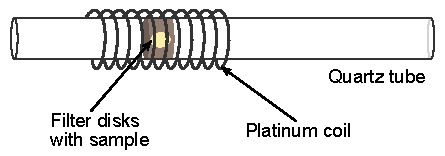
\includegraphics[width=\marginparwidth]{figures/quartz-tube}
	\caption{Schematic of a pyrolyzer quartz tube equipped with filter disks to absorb the liquid sample.}
	\label{fig:quartz-tube}
\end{marginfigure}

Prior to \ac{py-gc-ms} analysis, a sample aliquot of \SI{2}{\micro\liter} was applied onto the filter disk inside the quartz tube using a gastight \SI{10}{\micro\liter} syringe with \ac{ptfe} plunger\sidenote{Hamilton 1701 N with 26s gauge, Bonaduz, Switzerland.}. The quartz tube was transferred into the pyrolyzer using stainless steal tweezers to avoid any contamination, for instance, from nitrile or latex gloves. The pyrolyzer interface was held at \SI{300}{\degreeCelsius} and continuously flushed with \SI{20}{\milli\liter\per\minute} \ch{He} to evaporate remaining \ac{tcb} (boiling point: \SI{213}{\degreeCelsius}) and volatiles on-line while remaining below \ac{pe}, \ac{pp}, and \ac{ps} degradation onsets of \SIrange{310}{350}{\degreeCelsius} \citep{DavidIntroducing2019}. After \SI{3}{\minute}, the sample was flash pyrolyzed (\SI{10}{\kelvin\per\milli\second}) at \SI{750}{\degreeCelsius} for \SI{15}{\second}. The pyrolysis temperature was chosen following the manufacturer's recommendation to overcome the heat resistance of the pyrolyzer quartz tube ensuring complete thermal degradation of the polymers. The pyrolysates were transferred to the \ac{gc-ms} system via a passivated transfer line (\SI{350}{\degreeCelsius}). The \ac{ssl} injector was operated at \SI{300}{\degreeCelsius} with a split ratio of 1:10. The pyrolysates were separated on a \SI{30}{\meter}\,\texttimes\,\SI{0.25}{\milli\meter} capillary column (\SI{5}{\percent} phenyl-arylene, \SI{95}{\percent} dimethylpolysiloxane, \SI{0.25}{\micro\meter} film thickness)\sidenote{ZB-5MS, Phenomenex, Aschaffenburg, Germany.} connected to a \SI{2}{\meter} deactivated fused silica guard column\sidenote{Phenomenex, Aschaffenburg, Germany.}. The \ch{He} carrier gas flow was set at \SI{1.3}{\milli\liter\per\minute}. The \ac{gc} oven was programmed from \SI{40}{\degreeCelsius} (\SI{2}{\minute} hold) to \SI{300}{\degreeCelsius} at \SI{8}{\kelvin\per\minute} (\SI{50}{\minute} run time). The transfer line connecting the \ac{gc} with the \ac{ms} was kept at \SI{280}{\degreeCelsius}, and the \ac{ms} ion source (\ac{ei}, \SI{70}{\electronvolt}) was heated to \SI{230}{\degreeCelsius}.
The fore pressure of the \ac{ms} was checked to be \SI{<0.07}{\milli\bar}. The background intensity of \SI{28}{\mz} (atmospheric \ch{N2}) was supposed to be \num{<5e7} and the \ac{tic} \num{<e8}. Values exceeding these criteria indicated a leak in the system.

\subsection{Pyrolysate Identification and Calibration}

Pyrolysates were first screened in scan mode (\SIrange{50}{300}{\mz}) before switching to \ac{sim} of specific \si{\mz} ratios (\SI{100}{\milli\second} dwell time) as indicated in Figure~\ref{fig:py-sample} and Table~\ref{tab:py-products} and reported in previous research \citep{TsugePyrolysis2011,FischerSimultaneous2017,DumichenAnalysis2015}. \Ac{tic} pyrograms were evaluated using OpenChrom, version 1.4.0\sidenote{Lablicate, Hamburg, Germany.} \citep{WenigPostoptimization2011} with the NIST08 database for peak identification. The identified pyrolysates (Table~\ref{tab:py-products}) were abbreviated based on a modified ``lipid number'' notation in the form of $b$$C$:$D$($p_1$, $p_2$, \dots, $p_{D/2}$), in which $C$ is the total number of carbon atoms of the compound, $D$ denotes the number of double bonds, and their respective position $p$ is given in parentheses \citep{ZellesFatty1999}. The prefix $b$ specifies additional functional groups and their position in the carbon backbone, for example, 2Me for a methyl group or 2Ph for a phenyl moiety at the second carbon atom.

\begin{figure*}
	\centering
	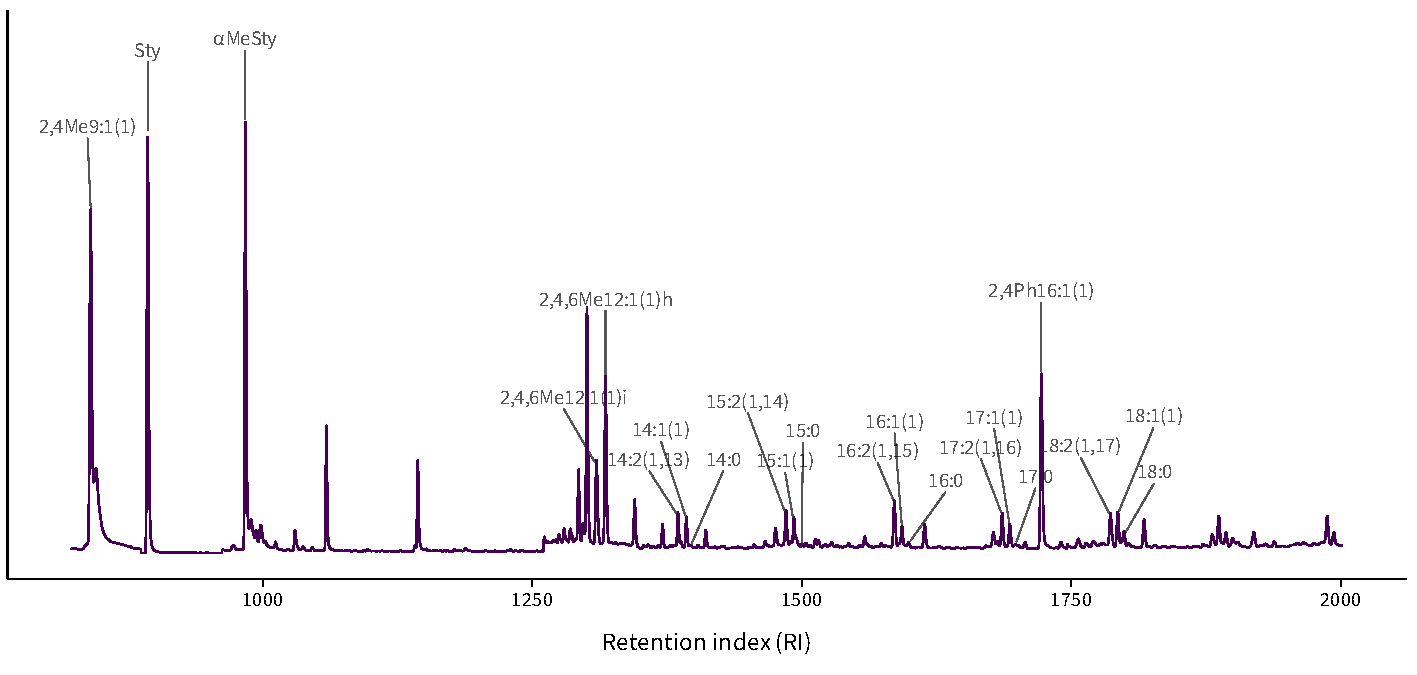
\includegraphics[width=\textwidth]{figures/py-sample}
	\caption[Sample pyrogram of \iac{pe}, \ac{pp}, and \ac{ps} mixture.]{Sample pyrogram of a polymer mixture containing each  \SI{150}{\milli\gram\per\kilo\gram} \ac{pe}, \ac{pp}, and \ac{ps}. Sty is not at scale. See Table~\protect\ref{tab:py-products} for details.}
	\label{fig:py-sample}
\end{figure*}

\begin{table*}
	\centering\footnotesize
	\caption{\Ac{pe}, \ac{pp}, and \ac{ps} pyrolysates analyzed for \ac{py-gc-ms} method development.}\label{tab:py-products}
	\begin{tabular}{llllS[table-format = 4]l}
		\toprule
		{Polymer} & {Pyrolysate} & {Full name} & {CAS} & {\Acs{ri}} & {\si{\mz}} \\
		\midrule
		PE & 14:2(1,13) & 1,13-Tetradecadiene & \cas[]{021964-49-8} & 1385 & \numlist[list-pair-separator = {, }]{82;95} \\
 & 14:1(1) & 1-Tetradecene & \cas[]{001120-36-1} & 1392 & \numlist[list-final-separator = {, }]{55;69;83}\textsuperscript{\textdaggerdbl} \\
 & 14:0 & Tetradecane & \cas[]{000629-59-4} & 1400 & \numlist[list-final-separator = {, }]{55;69;83}\textsuperscript{\textdaggerdbl} \\
 & 15:2(1,14) & 1,14-Pentadecadiene & \cas[]{021964-50-1} & 1485 & \numlist[list-pair-separator = {, }]{82;95} \\
 & 15:1(1) & 1-Pentadecene & \cas[]{013360-61-7} & 1493 & \numlist[list-final-separator = {, }]{55;69;83}\textsuperscript{\textdaggerdbl} \\
 & 15:0 & Pentadecane & \cas[]{000629-62-9} & 1500 & \numlist[list-final-separator = {, }]{55;69;83}\textsuperscript{\textdaggerdbl} \\
 & 16:2(1,15) & 1,15-Hexadecadiene & \cas[]{021964-51-2} & 1585 & \numlist[list-pair-separator = {, }]{82;95} \\
 & 16:1(1) & 1-Hexadecene & \cas[]{113032-42-1} & 1593 & \numlist[list-final-separator = {, }]{55;69;83}\textsuperscript{\textdaggerdbl} \\
 & 16:0 & Hexadecane & \cas[]{000544-76-3} & 1600 & \numlist[list-final-separator = {, }]{55;69;83}\textsuperscript{\textdaggerdbl} \\
 & 17:2(1,16) & 1,16-Heptadecadiene & \cas[]{021964-52-3} & 1686 & \numlist[list-pair-separator = {, }]{82;95} \\
 & 17:1(1) & 1-Heptadecene & \cas[]{006765-39-5} & 1693 & \numlist[list-final-separator = {, }]{55;69;83}\textsuperscript{\textdaggerdbl} \\
 & 17:0 & Heptadecane & \cas[]{000629-78-7} & 1700 & \numlist[list-final-separator = {, }]{55;69;83}\textsuperscript{\textdaggerdbl} \\
 & 18:2(1,17) & 1,17-Octadecadiene & \cas[]{013560-93-5} & 1787 & \numlist[list-pair-separator = {, }]{82;95} \\
 & 18:1(1) & 1-Octadecene & \cas[]{000112-88-9} & 1793 & \numlist[list-final-separator = {, }]{55;69;83}\textsuperscript{\textdaggerdbl} \\
 & 18:0 & Octadecane & \cas[]{000593-45-3} & 1800 & \numlist[list-final-separator = {, }]{55;69;83}\textsuperscript{\textdaggerdbl} \\
PP & 2,4Me9:1(1) & 2,4-Dimethyl-1-heptene & \cas[]{19549-87-2} & 841 & \numlist[list-pair-separator = {, }]{70;126} \\
 & 2,4,6Me12:1(1)i & 2,4,6-Trimethyl-1-nonene (isotactic) & \cas[]{55771-40-9} & 1307 & \numlist[list-pair-separator = {, }]{69;111} \\
 & 2,4,6Me12:1(1)h & 2,4,6-Trimethyl-1-nonene (heterotactic) & \cas[]{55771-40-9} & 1316 & \numlist[list-pair-separator = {, }]{69;111} \\
PS & Sty & Styrene & \cas[]{100-42-5} & 895 & \numlist[list-pair-separator = {, }]{78;104} \\
 & $\alpha$MeSty & $\alpha$-Methylstyrene & \cas[]{98-83-9} & 981 & \numlist[list-pair-separator = {, }]{103;118} \\
 & 2,4Ph16:1(1) & 2,4-Diphenyl-1-butene & \cas[]{16606-47-6} & 1721 & \numlist[list-pair-separator = {, }]{91;208} \\
 & 2,4,6Ph24:1(1) & 2,4,6-Triphenyl-1-hexene & \cas[]{18964-53-9} & 2438 & \numlist[list-pair-separator = {, }]{91;207} \\
		\bottomrule
		\multicolumn{6}{l}{\acs{ri} = \acl{ri}; \textsuperscript{\textdaggerdbl} used for screening only.} \\~
	\end{tabular}
	\forceversofloat
\end{table*}

The peaks were automatically integrated from the valley between the peaks to the horizontal baseline using a sliding window size of 3~scans and a minimum \ac{snr} of~7.
Calibration series of \SIrange{5}{150}{\micro\gram\per\milli\liter} mixed \ac{pe}, \ac{pp}, and \ac{ps} standards were pyrolyzed together with \numrange{3}{5} blanks (\SI{0}{\micro\gram\per\milli\liter} in \ac{tcb}).
\Acp{lod} and \acp{loq} were calculated using Equations~\ref{eq:lod} and \ref{eq:loq} as described in Chapter~\ref{ch:tga-ms-method}.
%\Acp{lod} and \acp{loq} were calculated using Equations~\ref{eq:lod} and \ref{eq:loq}, respectively, in accordance with the German standard \citet{DIN32645Chemical2008} as implemented in the R package ``envalysis''\sidenote{The package source is available at \doi{10.5281/zenodo.1240305}} (version 0.3.3).
%
%\begin{equation}
%\mathrm{LOD} = \frac{\sigma_\mathrm{blank}}{a} \cdot t_{n-1;0.01} \sqrt{n^{-1} + m^{-1}}
%\label{eq:lod}
%\end{equation}
%
%\begin{equation}
%\mathrm{LOQ} = k \cdot \frac{\sigma_{xy}}{a} \cdot t_{n-2;0.01} \sqrt{n^{-1} + m^{-1} + \frac{(\mathrm{LOQ}-\overline{x})^2} {S_{xx}}}
%\label{eq:loq}
%\end{equation}
%
%Therein, $\sigma_\mathrm{blank}$ is the standard deviation of integrated peak areas from blanks, $\sigma_{xy}$ is the residual standard deviation, and $a$ is the slope of the calibration curve. $t$ is the \SI{99}{\percent} percentile of the Student's $t$ distribution with $n - 1$ and $n - 2$ degrees of freedom, $n$ as the total number of measurements, and $m$ as the number of replicates. $k = 3$ is the recommended certainty factor for the \ac{loq}; $\overline{x}$ is the arithmetic mean of all standard concentrations, and $S_{xx}$ is the sum of squares of $x$. Note that calculating the \ac{loq} is an iterative process with $\mathrm{LOQ} = k \cdot \mathrm{LOD}$ as initial value.
Instrumental \acp{lod} were calculated by multiplication of the respective \acp{lod} with the injection volume of \SI{2}{\micro\liter}. Method \acp{lod} were estimated by dividing \acp{lod} by the extraction volume of \SI{8}{\milli\liter} and multiplying it with the extracted soil mass (\SI{4}{\gram}).

\subsection{Method Validation}

At the beginning of each week, a fresh calibration series was prepared. Sample measurements of the following days were bracketed with \SI{100}{\micro\gram\per\milli\liter} standards to correct for inter-day variations in peak intensities. Corrected peak areas were then used for quantification.

In line with IUPAC recommendations \citep{CurrieNomenclature1995}, the intra-day repeatability of the \ac{py-gc-ms} method was verified by measuring a sequence of \SI{150}{\micro\gram\per\milli\liter} standards ($n = 10$) and determining \acp{rsd} of peak areas. A linear model was fitted to the data to check if the peak areas changed significantly during the day. Inter-day variability was estimated from two \SI{150}{\micro\gram\per\milli\liter} standard samples repeatedly measured for eight days.

In order to test whether \ac{pe}, \ac{pp}, and \ac{ps} selectively decompose into their respective pyrolysates without interfering with each other, successive measurements of \SI{150}{\micro\gram\per\milli\liter} mixed polymer standards were compared with standards containing each individual polymer. Furthermore, potential interferences from soil matrix and non-target plastics (\ac{pet}, \ac{pmma}, \ac{pvc}, and \ac{twp}) were assessed. Differences in peak areas of pyrolysates were statistically evaluated using \acp{anova} with Bonferroni\-/adjusted Tukey tests for post\-/hoc multiple comparisons. \Acp{anova} were checked for normality and homoscedasticity of residuals using quantile\--quantile and residual vs. fitted plots.
The same statistical tools were applied to compare the various extraction and cleanup methods for \ac{pe}, \ac{pp}, and \ac{ps} from different soil types with one another.
Data analysis was performed using R statistical software (version 3.6.1)\sidenote{All data and R code to reproduce data processing and statistical tests are publicly available at \doi{10.6084/m9.figshare.11861664}.}.
Results are given as mean\,$\pm$\,\ac{sd}.

\section{Results and Discussion}

\subsection{Polymer Quantification}

From the initial screening set of 22~pyrolysates (Table~\ref{tab:py-products}), six compounds performed best in terms of linearity (adj. $R^2 >$ \num{0.996}) within the calibration range, \acp{lod}, and \acp{loq} (Figure~\ref{fig:py-calibration} and Table~\ref{tab:py-calibration}). \Acp{lod} were below the lowest standard of \SI{5}{\micro\gram\per\milli\liter} for the \ac{pe} $n$-alkadienes 15:2(1,14) and 17:2(1,16) detected via \SIlist{82;95}{\mz}. 18:2(1,17) produced \iac{lod} of \SI{11.3}{\micro\gram\per\milli\liter}. The \acp{loq} ranged between \SIrange[range-phrase = { and }]{25}{54}{\micro\gram\per\milli\liter}.
For \ac{pp}, only 2,4Me9:1(1) was quantifiable (\SIlist{70;126}{\mz}) with \iac{lod} and \ac{loq} of \SIlist{43.2;46.7}{\micro\gram\per\milli\liter}, respectively.
Sty and $\alpha$MeSty were the most indicative pyrolysates for \ac{ps} and detected via \SIlist{78;104}{\mz} and \SIlist{103;118}{\mz}, respectively. Their adj. $R^2$s, \acp{lod}, and \acp{loq} were similar to \ac{pe} pyrolysates.

\begin{figure*}
	\centering
	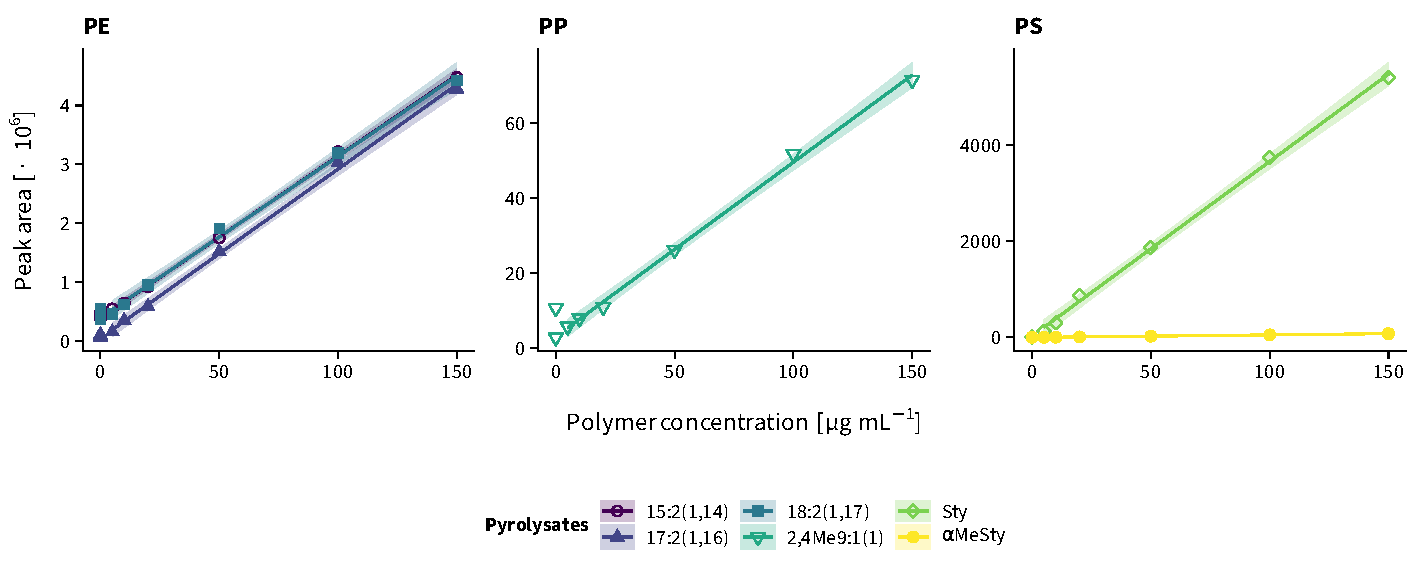
\includegraphics[width=\textwidth]{figures/py-calibration}
	\caption[\Ac{py-gc-ms} calibration curves of \ac{pe}, \ac{pp}, and \ac{ps} standards in \acs{tcb}.]{\Ac{py-gc-ms} calibration curves of \ac{pe}, \ac{pp}, and \ac{ps} standards in \ac{tcb}; see Table~\protect\ref{tab:py-calibration} for parameters.}
	\label{fig:py-calibration}
\end{figure*}

\begin{table}[b]
	\centering\footnotesize
	\caption{\Ac{py-gc-ms} calibration parameters of pyrolysates selected for quantification.}\label{tab:py-calibration}
	\begin{tabular}{llS[table-format = 8]S[table-format = 8]S[table-format = 1.4]S[table-format = 2.1]S[table-format = 2.1]}
		\toprule
		{Polymer} & {Pyrolysate} & {Intercept} & {Slope} & {adj. $R^2$} & {\Acs{lod}} & {\Acs{loq}} \\
		& & & & & [\si{\micro\gram\per\milli\liter}] & [\si{\micro\gram\per\milli\liter}] \\
		\midrule
		PE & 15:2(1,14) & 384440 & 27563 & 0.9992 & 4.8 & 25.7 \\
 & 17:2(1,16) & 40501 & 28782 & 0.9980 & 2.5 & 38.6 \\
 & 18:2(1,17) & 391786 & 27423 & 0.9962 & 11.3 & 53.4 \\
PP & 2,4Me9:1(1) & 2987986 & 464559 & 0.9971 & 43.2 & 46.7 \\
PS & Sty & 26306594 & 36246576 & 0.9975 & 0.5 & 43.3 \\
 & $\alpha$MeSty & -860185 & 527700 & 0.9986 & 1.6 & 33.1 \\

		\bottomrule
	\end{tabular}
\end{table}

Taking into account the \SI{2}{\micro\liter} injection volume, instrumental \acp{lod} were \SIrange{1}{86}{\nano\gram}. This is at least \num{2.5} times lower than most recent advances in \ac{pe}, \ac{pp}, and \ac{ps} method developments with \ac{ted-gc-ms} and microfurnace \ac{py-gc-ms} \citep{DuemichenAutomated2019,FischerMicroplastics2019,DierkesQuantification2019}. Note that \citet{DierkesQuantification2019} reported \acp{loq} calculated from blanks, which is usually defined as \ac{lod} (Equation~\ref{eq:lod}). While \citet{DuemichenAutomated2019,DierkesQuantification2019} used the same indicator pyrolysates for quantification as we did but on different \si{\mz} ratios, \citet{FischerMicroplastics2019} chose $n$-alkanes, $n$-alkenes, and the \ac{ps} trimer 2,4,6Ph24:1(1).

All these studies have in common that they relied on a very sensitive microscale to weigh several nanograms of solid polymer directly into pyrolyzer sample cups or to quantitatively transfer a representative aliquot of solid mixture. To facilitate the heat transfer of the pyrolyzer filament or microfurnace into the sample, the lowest sample amount possible is typically aimed for. However, the lower the amount to be weighed, the higher the relative weighing error becomes and the more challenging it is to obtain a homogeneous mixture. So far, this has been one of the major drawbacks of \ac{py-gc-ms} \citep{FischerMicroplastics2019}.
When combining \ac{py-gc-ms} with prior dissolution of polymers in an appropriate solvent such as \ac{tcb}, stock solutions can be easily handled, quantitatively diluted or preconcentrated, and transferred directly into the pyrolyzer quartz tubes. Dissolution in \ac{tcb} therefore allows for constantly pyrolyzing the same but low amount of sample. Absorbing the \ac{tcb} solution into the quartz filter disks inside the quartz tube further ensures the optimal alignment of the sample with the pyrolyzer filament and thereby enabling more accurate and reproducible pyrolyses down to the nanogram range. Trying to further improve \acp{lod} and \acp{loq} by increasing sample injection volumes could therefore be at the expense of measurement accuracy.

\subsection{Repeatability}

The \acp{rsd} of \ac{pe} indicator pyrolysates were \SIrange{3.4}{4.5}{\percent} without showing any trend of systematically increasing or decreasing peak intensities during a one-day series of $n = 10$ standard measurements (Figure~\ref{fig:py-repeatability}, $p > 0.529$, linear model); this is intra-day variability. By contrast, inter-day variability was \SIrange{15.2}{17.9}{\percent}. The \ac{pp} pyrolysate 2,4Me9:1(1) produced a stable ($p = 0.728$, linear model) intra-day \ac{rsd} of \SI{7.2}{\percent}, and an inter-day \ac{rsd} of \SI{10.4}{\percent}. With \SIlist{3.2;4.2}{\percent} of intra-day variability, the \acp{rsd} of \ac{ps} pyrolysates Sty and $\alpha$MeSty were in the same range as \ac{pe}.  However, Sty showed a statistically significant tendency to decrease in signal intensity by \SI{0.88}{\percent} per measurement ($p = 0.002$, linear model), while $\alpha$MeSty increased by \SI{1.05}{\percent} ($p = 0.020$, linear model). With respect to the \acp{rsd} of the measurement series, these changes are deemed negligible if peak intensities are corrected with bracketing standards measured in the beginning and at the end of each day. This also applies to the inter-day variabilities of Sty and $\alpha$MeSty which were  \SIlist{13.9;16.5}{\percent}.

\begin{figure*}[t]
	\centering
	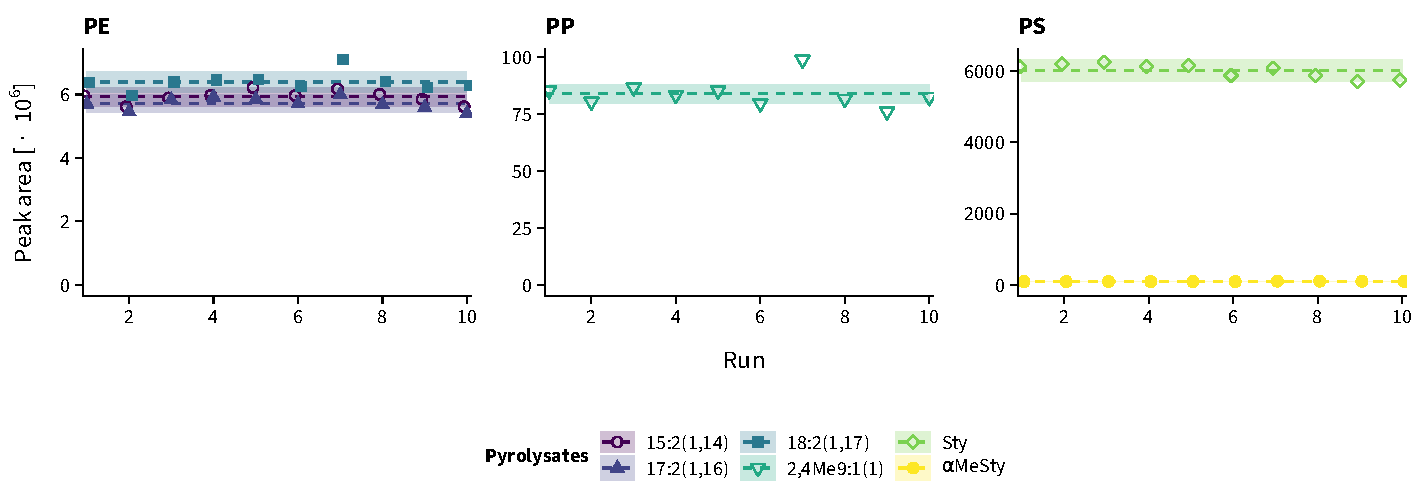
\includegraphics[width=\textwidth]{figures/py-repeatability}
	\caption[Repeatability of \ac{py-gc-ms} measurements.]{Repeatability of \ac{py-gc-ms} measurements ($n = 10$) with means (dashed lines) and \SI{+-5}{\percent} \acs{rsd} bands.}
	\label{fig:py-repeatability}
\end{figure*}

Measurement repeatability was in line with comparable studies. \Ac{ps} analysis via \ac{lc-ms} with an atmospheric pressure photoionization source, for instance, resulted in an intra- and inter-day repeatability of \SIrange{1.8}{2.4}{\percent} and \SIrange{15.5}{25.6}{\percent}, respectively ($n = 5$) \citep{SchirinziTrace2019}. With \ac{ted-gc-ms}, \citet{DuemichenAutomated2019} achieved \acp{rsd} ranging from \SIrange[range-phrase = { to }]{6}{12}{\percent} for various \ac{pp} pyrolysates. The authors suggested using an internal standard to further optimize \acp{rsd}. \citet{FischerMicroplastics2019} used androstane, deuterated anthracene, 9-dodecyl-1,2,3,4,5,6,7,8-octahydro anthracene, and cholanic acid for internal standardization of \ac{pe}, \ac{pet}, polycaprolactam, and \ac{ps}. Since those internal standards are not polymers, they probably behave differently than the polymer analytes when heated to typical pyrolysis temperatures of \SIrange{600}{800}{\degreeCelsius}. Particularly polycyclic aromatic hydrocarbons such as anthracene are thermally stable and more likely to evaporate instead of thermally decomposing along with the polymer analytes. Accordingly, \citet{FischerMicroplastics2019} reported that the deuterated anthracene might have interacted with the inner surface of the pyrolyzer which eventually decreased repeatability. Though expensive, deuterated plastics \citep{DierkesQuantification2019} or specialized polymers like \ac{pedot} typically used in semiconductor industry could be promising alternatives since they decompose in the same temperature range as the polymer analytes \citep{JinThermal2013}. The use of an appropriate internal standards for routine \ac{py-gc-ms} analyses will be evaluated in future studies (Chapter~\ref{ch:screening}).

\subsection{Selectivity of Indicator Pyrolysates}\label{sec:selectivity}

\Ac{pe} pyrolyzes into $n$-alkanes, $n$-alkenes, and $n$-alkadienes of decreasing chain length (Figure~\ref{fig:py-sample}). In the pyrogram sections given in Figure~\ref{fig:py-selectivity1}, the first peaks of these triplets are the $n$-alkadienes used for quantification (\acp{ri} $=$ \numlist{1486;1686;1786}, Table~\ref{tab:py-products}) followed by their respective $n$-alkenes (\acp{ri} $+$ \num{7}). Note that the $n$-alkanes (\acp{ri} $=$ \numlist{1500;1700;1800}) were low in intensity due to \si{\mz} ratios optimized for $n$-alkadienes.
Regardless of pyrolyzing a \SI{150}{\micro\gram\per\milli\liter} \ac{pe} standard individually or in a mixture with \ac{pp} and \ac{ps}, the $n$-alkadiene peaks aligned accurately with one another, while signals from \ac{pp} or \ac{ps} were negligible particularly for 15:2(1,14) and 17:2(1,16). 18:2(1,17) was slightly interfered by \ac{pp} and \ac{ps} although this was not statistically significant (Figure~\ref{fig:py-selectivity2}; $p = 1$, Tukey). For 15:2(1,14), however, triplicate measurements of the polymer mixture were on average about \SI{15}{\percent} lower than pure \ac{pe} ($p < 0.001$, Tukey). In general, 17:2(1,16) showed the least interferences with background signals from pure \ac{pp} and \ac{ps} being comparable to blank measurements ($p = 1$, Tukey).
The \ac{pp} indicator pyrolysate 2,4Me9:1(1) at \ac{ri} \num{841} was about \SI{10}{\percent} lower in intensity when pure \ac{pp} was pyrolyzed compared to the polymer mixture ($p = 0.057$, Tukey). This suggests a minor interference from \ac{pe} that may have originated from the peak shoulder at \ac{ri} 845 and a slightly higher but statistically insignificant background noise from \ac{pe} and \ac{ps} ($p = 1$, Tukey).
In comparison to that, Sty and $\alpha$MeSty from \ac{ps} pyrolysis were both selective in terms of showing no interference from \ac{pe} and \ac{pp} ($p < 0.001$, Tukey). For its lower variation compared to Sty, $\alpha$MeSty may be favorably used for \ac{ps} quantification.

\begin{figure*}[t]
	\centering
	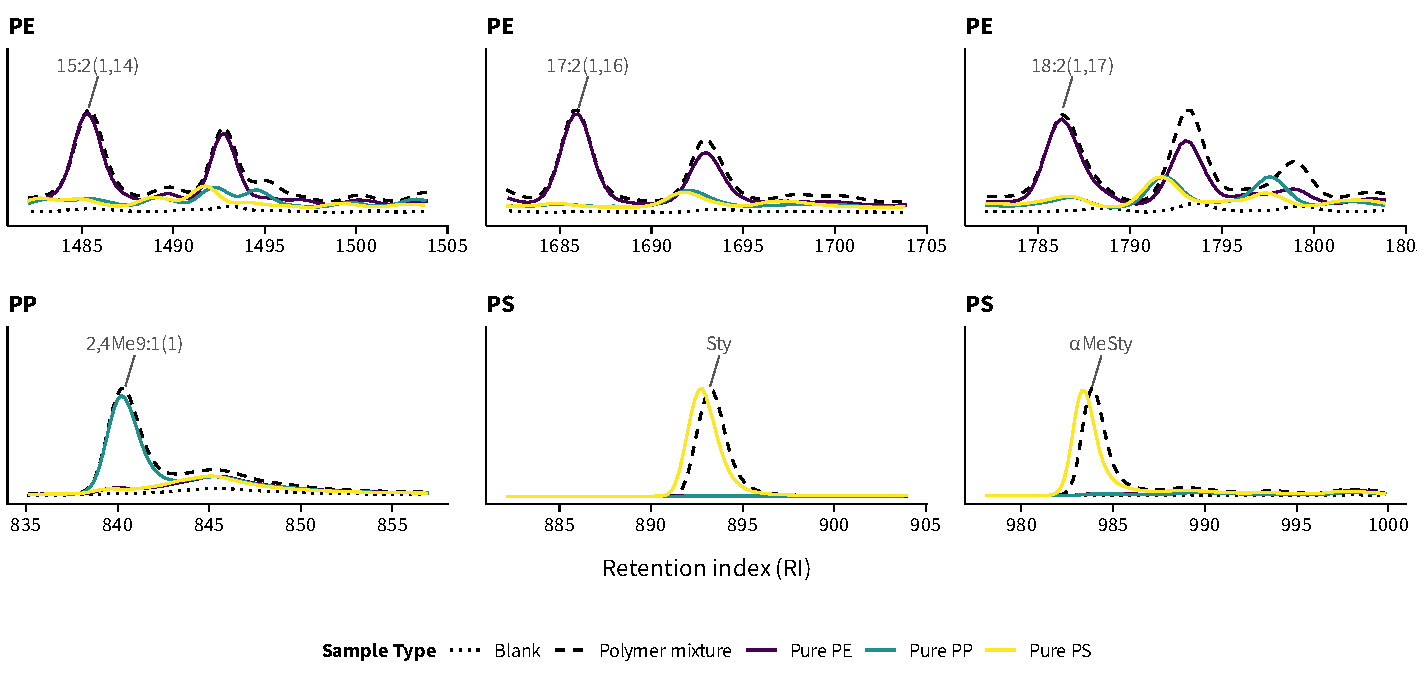
\includegraphics[width=\textwidth]{figures/py-selectivity1}
	\caption[Pyrogram sections of \ac{pe}, \ac{pp}, and \ac{ps} pyrolysates.]{Pyrogram sections of \ac{pe}, \ac{pp}, and \ac{ps} pyrolysates obtained by analyzing each individual polymer or a mixture of all three polymers (\SI{150}{\micro\gram\per\milli\liter}).}
	\label{fig:py-selectivity1}
	\forceversofloat
\end{figure*}

\begin{figure*}[b]
	\centering
	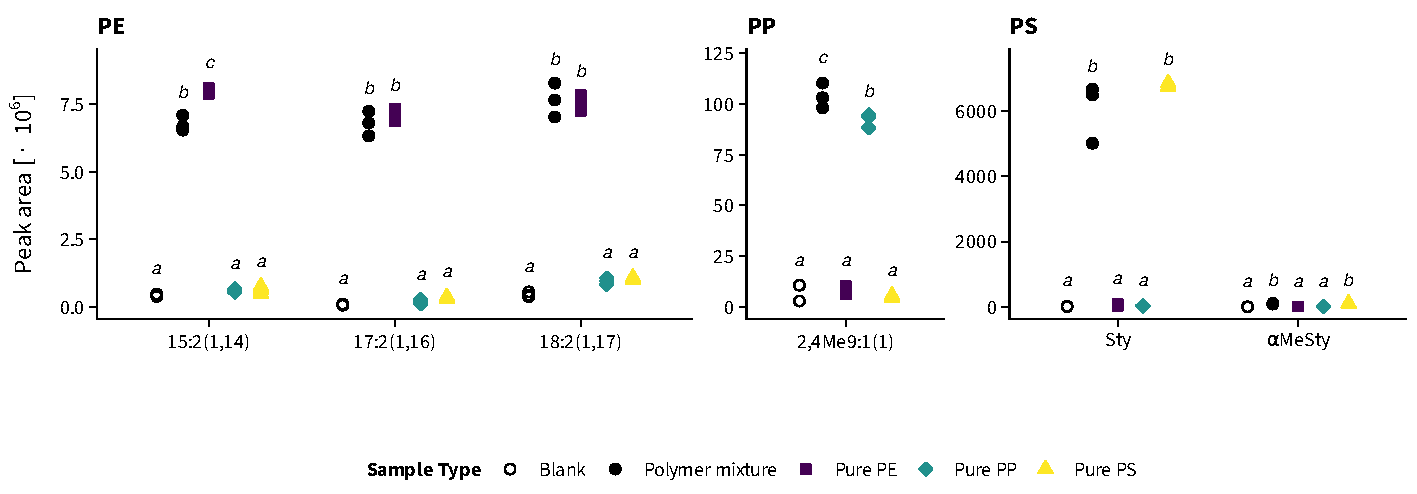
\includegraphics[width=\textwidth]{figures/py-selectivity2}
	\caption[Peak areas of \ac{pe}, \ac{pp}, and \ac{ps} pyrolysates.]{Peak areas of \ac{pe}, \ac{pp}, and \ac{ps} pyrolysates measured individually or in a mixture of all three polymers (\SI{150}{\micro\gram\per\milli\liter}); different letters (in italics) indicate significant differences between sample types for each pyrolysate ($p < 0.05$, Tukey).\\~}
	\label{fig:py-selectivity2}
	\forceversofloat
\end{figure*}

To our knowledge, the possibility of polymers analyzed together and interfering with each other by formation of identical or chromatographically inseparable pyrolysates has so far only been described by \citet{FischerSimultaneous2017}. However, the authors neither tested potential interferences in their \ac{py-gc-ms} setup nor suggested a certain approach to counteract them. With our experimental design, we were able to show that \ac{pe}, \ac{pp}, and \ac{ps} can be selectively analyzed in a polymer mixture without interfering with each other by more than \SI{10}{\percent} at equal concentrations. Especially \ac{pp} quantified via 2,4Me9:1(1) may be slightly overestimated when \ac{pe} is present in large quantities. But since the \ac{pe} pyrolysate 17:2(1,16) was particularly robust against background signals from \ac{pp} or \ac{ps}, it would be possible to correct the overestimated \ac{pp} content for its \ac{pe} share.

\subsection{Matrix Interferences}\label{sec:matrix-interferences}

Extracting LUFA~2.2 and RefeSol 06-A with \ac{tcb}, but without adding plastic, resulted in background signals equivalent to \SIlist{70(10);31(4)}{\milli\gram\per\kilo\gram} \ac{pe}, respectively (Table~\ref{tab:py-matrix}). Interestingly, addition of the non-target plastics \ac{pet}, \ac{pvc}, \ac{pmma}, and \ac{twp} to LUFA~2.2 soil did not increase matrix interferences. With \SI{700(200)}{\milli\gram\per\kilo\gram}, the matrix-induced background signal in WR soil was about \numrange{10}{20} times higher than in LUFA~2.2. For soils with \iac{Corg} content exceeding \SI{2}{\percent}, namely RefeSol 06-A and WR, a prior cleanup step with methanol doubled \ac{pe} background levels. Similarly, Fenton digestion of WR soil resulted in matrix interferences equivalent to \SI{1000(200)}{\milli\gram\per\kilo\gram} \ac{pe}. Only flocculation with \ch{KAl(SO_4)_2} considerably reduced background levels to \SI{400(200)}{\milli\gram\per\kilo\gram}. Regardless of the extraction method and pretreatment, procedural blanks were below the estimated method \acp{lod} of \SI{5}{\milli\gram\per\kilo\gram}.
The \ac{pp} background extracted with \ac{tcb} was not detectable except for WR soil (\SI{100(100)}{\milli\gram\per\kilo\gram}). Similar to \ac{pe}, \ac{pp} levels doubled when applying a prior methanol cleanup step. However, \ch{KAl(SO_4)_2} flocculation and Fenton digestion were able to reduce matrix interferences below the \ac{lod}.
\Ac{ps} background levels in LUFA~2.2 soil were below the method \ac{lod} of \SI{3.2}{\milli\gram\per\kilo\gram}. In line with \ac{pe} and \ac{pp}, \ac{ps} contents slightly increased with the \ac{Corg} content of the soil. With respect to \acp{sd}, neither the methanol cleanup nor Fenton digestion changed the matrix-induced background considerably while \ch{KAl(SO4)2} decreased matrix interferences to non-detectable levels.

\begin{table*}
	\centering\footnotesize
	\caption[Matrix interferences of different soil types.]{Matrix interferences of different soil types (mean\,$\pm$\,\ac{sd}).}\label{tab:py-matrix}
	\begin{tabular}{llS[table-format = 4(3)]S[table-format = 4(3)]S[table-format = 4(3)]S[table-format = 4(3)]}
		\toprule
		{Polymer} & {Soil} & \multicolumn{2}{l}{{Extraction procedure} [\si{\milli\gram\per\kilo\gram}]} \\
		\cmidrule(lr){3-6}
		& & {\Acs{tcb} only} & {Methanol cleanup} & {\ch{KAl(SO4)2} flocculation} & {Fenton digestion}\\
		\midrule
		PE & LUFA 2.2 & 70(10) &  &  &  \\
 & LUFA 2.2\textsuperscript{\textasteriskcentered} & 70(7) &  &  &  \\
 & RefeSol 06-A & 31(4) & 70(20) &  &  \\
 & WR & 700(200) & 1300(100) & 400(200) & 1000(200) \\
PP & LUFA 2.2 & 0(200) &  &  &  \\
 & LUFA 2.2\textsuperscript{\textasteriskcentered} & 0(100) &  &  &  \\
 & RefeSol 06-A & 0(0) & 32(100) &  &  \\
 & WR & 100(100) & 200(100) & 0(0) & 0(0) \\
PS & LUFA 2.2 & 2(4) &  &  &  \\
 & LUFA 2.2\textsuperscript{\textasteriskcentered} & 4(3) &  &  &  \\
 & RefeSol 06-A & 20(30) & 1(1) &  &  \\
 & WR & 7(3) & 12(4) & 0(4) & 8(3) \\

		\bottomrule
		\multicolumn{6}{p{.75\textwidth}}{\textsuperscript{\textasteriskcentered} with \SI{50}{\milli\gram\per\kilo\gram} non-target polymers (\SI{19}{\percent} \ac{pet}, \SI{11}{\percent} \ac{pmma}, \SI{41}{\percent} \ac{pvc}, and \SI{29}{\percent} \ac{twp}); indicator pyrolysates were 17:2(1,16) for \ac{pe}, 2,4Me9:1(1) for \ac{pp}, and $\alpha$MeSty for \ac{ps}.}
	\end{tabular}
\end{table*}

The matrix interferences identified in our study were generally comparable to those reported in previous thermoanalytical studies: \citet{DierkesQuantification2019} detected matrix interferences equivalent to \SIlist{140;210;50}{\milli\gram\per\kilo\gram} \ac{pe} in an artificial, inert matrix spiked with \SI{3}{\percent} of wood, leafs, or humic acids, respectively. The authors applied \ac{ase} with methanol and \ac{thf} prior to \ac{py-gc-ms} quantification via 15:2(1,14). Similarly, \citet{FischerSimultaneous2017} found their \ac{pe} and \ac{ps} pyrolyses affected by chitin, wood, wool, and cellulose, however, without quantifying potential interferences. For two natural soils with unreported \ac{Corg}, \SIrange{790}{850}{\milli\gram\per\kilo\gram} \ac{pe}, \SI{40}{\milli\gram\per\kilo\gram} \ac{pp}, and \SIrange{40}{50}{\milli\gram\per\kilo\gram} \ac{ps} were detected \citep{DierkesQuantification2019}. The question whether these levels came from matrix interferences or a contamination with plastic debris remained unresolved. By contrast, \citet{DumichenAnalysis2015} applied \ac{ted-gc-ms} and found that soil matrix with an unspecified \ac{Corg} did not induce any interferences. Since \citet{DumichenAnalysis2015,DumichenFast2017} determined \ac{pe} in a concentration range approximately three orders of magnitude higher than we did, contrasting findings are most likely attributed to the higher sensitivity of our \ac{py-gc-ms} setup. A comparison with existing microspectoscopic methods \citep{ScheurerMicroplastics2018,PiehlIdentification2018} remains difficult since results are typically reported as particle counts. Conversions from particle counts and sizes to mass concentrations are error-prone for the high uncertainties associated with the underlying assumptions on particle shapes and density distributions. That being said, background levels from \ac{ftir} analyses of Swiss floodplains were estimated at \SIrange{0}{55}{\milli\gram\per\kilo\gram} and averaged \SI{5}{\milli\gram\per\kilo\gram}, which is \numrange{1.2}{15} times lower than the matrix interferences identified in our study.

Besides a facilitated sample handling, dissolution of \ac{pe}, \ac{pp}, and \ac{ps} in \ac{tcb} offers the advantage of restricting the amount of other polymers and interfering matrix being dissolved along with the analytes and transferred into the \ac{py-gc-ms} system. Apart from our three target polymers, \ac{tcb} is recommended as \ac{sec} solvent only for poly(ethylene-vinyl acetate), polythiophene, and other polyolefins \citep{BivensPolymertoSolvent2016}. In addition, only compounds thermally decomposing between \SIrange[range-phrase = { and }]{300}{750}{\degreeCelsius} were passed to our \ac{gc-ms}, which may have further reduced the potential for interferences.

In spite of that, we found particularly high matrix interferences for \ac{pe} in WR soil, a pristine forest soil with \SI{5.16}{\percent} \ac{Corg}. The two agricultural soils with \SI{<2.5}{\percent} \ac{Corg} showed considerably lower background signals.
This is not surprising since up to \SI{9}{\percent} of soil \ac{Corg} consists of \ch{(CH2)_{$n$}} chains of \numrange{25}{30} units \citep{HuPoly2000} as, for example, present in suberins, cutins, or microbial cell membranes. Based on the \ac{Corg} of our reference soils, this fraction could potentially induce interferences equivalent to \SIrange{1500}{4500}{\milli\gram\per\kilo\gram} \ac{pe}. Just by using \ac{tcb} as an extraction agent, we were able to reduce potential interferences by a factor of \numrange{5}{20}. In comparison with that, prior Fenton digestion or methanol cleanup rather mobilized than removed interfering matrix constituents, for instance by cell lysis, which was indicated by elevated \ac{pe} background levels from both pretreatments. The differences between both pretreatments may be attributed to the oxidization potential of Fenton reagent that most likely made available but at the same time removed a larger fraction of interfering matrix constituents than methanol.
Here, existing \ac{ase} applications with three rinsing cycles of \SI{15}{\milli\liter} methanol per \SI{1}{\gram} of sample at \SI{100}{\degreeCelsius} \citep{FullerProcedure2016,DierkesQuantification2019} may be superior to our simplified batch setup. But matrix interferences from such extraction setups have not been quantified for organic rich soils yet.
Besides that, it cannot be excluded that reference soils may have been contaminated with plastic debris on-site or during packaging and shipping, thereby, mistaking a potential plastic contamination for matrix interferences. This could only be assessed by characterizing soil organic matter fractions from soil databases dating back to times before the introduction of today's consumer plastics. Based on these findings, further efforts should be made to reduce interferences from specific soil constituents, for instance by using an advanced flotation and filtration apparatus, molecular sieves, dispersive \ac{spe}, or on-line transesterification and evaporation of lipid-like substances with \ch{BF3} or \ac{tmsh} prior pyrolysis. Moreover, further research will need to test alternative solvent mixtures to extend the applicability of our \ac{py-gc-ms} approach to a wider range of polymer types.

\subsection{Plastic Recovery from Soil}

As outlined above, matrix interferences equivalent to \SI{>400}{\milli\gram\per\kilo\gram} \ac{pe} exceeded the spiked polymer content by a factor of \numrange{2}{4}. In those cases, the calculation of matrix-corrected recoveries was not meaningful and data were thus excluded from further examination (Figure~\ref{fig:py-recovery}).
\Ac{pe} recovered from LUFA~2.2 with \ac{tcb} only ranged from \SIrange[range-phrase = { to }]{80}{110}{\percent}. The recoveries were independent of the spiking level, and the addition of non-target polymers did not influence the recovery of \ac{pe}. For RefeSol 06-A, recoveries with \ac{tcb} were slightly lower than in LUFA~2.2 (\SIlist{61;70}{\percent}). The methanol cleanup decreased the recovery to \SIlist{26;55}{\percent}. Due to the high matrix interferences discussed in Section~\ref{sec:matrix-interferences}, \ac{pe} recoveries from WR soil could only be evaluated for samples flocculated with \ch{KAl(SO4)2} prior to \ac{tcb} extraction, and the recovery was very low (\SI{10(10)}{\percent}).
Extracting \ac{pp} from LUFA~2.2 and RefeSol 06-A soil using \ac{tcb} yielded recoveries of \SIrange{100}{160}{\percent}. At \SI{50}{\milli\gram\per\kilo\gram} spiking level, recoveries were higher and varied more than at \SI{250}{\milli\gram\per\kilo\gram}. In line with \ac{pe}, the methanol pretreatment decreased recoveries to \SIlist{63;80}{\percent}. In WR soil, only \SI{30(20)}{\percent} of \ac{pp} were recovered after \ch{KAl(SO4)2} flocculation. Prior Fenton digestion increased recoveries to \SIlist{110;140}{\percent}.
\Ac{ps} recoveries ranged from \SIrange[range-phrase = { to }]{77}{119}{\percent}, except for the Fenton digestion of WR soil (\SI{130(10)}{\percent}) and \ac{tcb} extraction of RefeSol 06-A at the lower spiking level of \SI{50}{\milli\gram\per\kilo\gram} (\SI{46(7)}{\percent}).

\begin{figure*}[t]
	\centering
	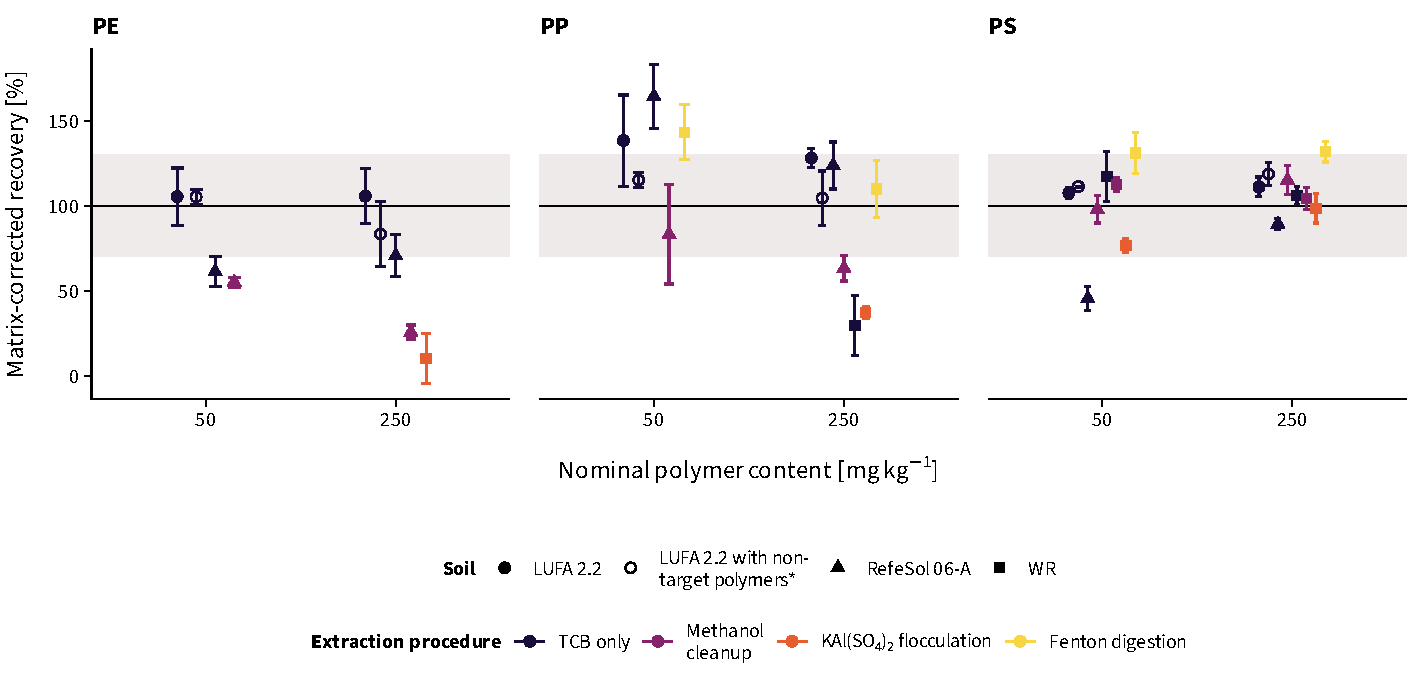
\includegraphics[width=\textwidth]{figures/py-recovery}
	\caption[Recoveries of \ac{pe}, \ac{pp}, and \ac{ps} from different soil types corrected for matrix interferences.]{Recoveries of \ac{pe}, \ac{pp}, and \ac{ps} from different soil types (mean\,$\pm$\,\ac{sd}) corrected for matrix interferences (Table~\protect\ref{tab:py-matrix}); the gray band marks the \SIrange{70}{130}{\percent} range acceptable for recovery experiments; \textsuperscript{\textasteriskcentered} \SI{50}{\milli\gram\per\kilo\gram} consisting of \SI{19}{\percent} \ac{pet}, \SI{11}{\percent} \ac{pmma}, \SI{41}{\percent} \ac{pvc}, and \SI{29}{\percent} \ac{twp}.}
	\label{fig:py-recovery}
\end{figure*}

In summary, \ac{tcb} extractions without any pretreatment performed best (\SIrange{70}{128}{\percent} recovery), particularly at \SI{250}{\milli\gram\per\kilo\gram} spiking level from soils with less than \SI{2.5}{\percent} \ac{Corg}. \Ac{pp} contents were slightly overestimated due to the aforementioned interference with \ac{pe} (Section~\ref{sec:selectivity}). Although \ch{KAl(SO4)2} effectively immobilized interfering matrix constituents, it concomitantly reduced \ac{pe} and \ac{pp} recoveries. This was potentially due to matrix floccules entrapping plastic debris, hence making it inaccessible to \ac{tcb} extraction. Similarly, low recoveries resulting from the methanol cleanup were most likely attributed to the discarding of supernatant methanol after rinsing, which probably also removed some plastic debris from the soil. Interestingly, prior Fenton digestion led to elevated recoveries, which contrasts \citet{HurleyValidation2018} who found Fenton reagent performing best in terms of organic matter removal and preservation of plastic particles prior to \ac{ftir} imaging. However, our findings are in line with previous thermoanalytical studies that obtained recoveries of \SIrange{80}{130}{\percent} when extracting \ac{pe}, \ac{pp}, and \ac{ps} with \ac{dcm} and \ac{thf} from solid matrices after an initial methanol cleanup \citep{FullerProcedure2016,DierkesQuantification2019}. In contrast to our study, \citet{FullerProcedure2016} used about \numrange{20}{100} times higher spiking levels (\SI{5}{\gram\per\kilo\gram}) and \citet{DierkesQuantification2019} extracted \SIlist{50;750}{\milli\gram\per\kilo\gram} microplastics from an artificial sample containing \SI{3}{\percent} humic acids in sea sand. In such an artificial matrix, interferences are less likely to occur than in natural soil with its large variety of substance classes like natural polymers, lipids, or proteins.

\section{Conclusions}

Dissolving the three most environmentally relevant polymers \ac{pe}, \ac{pp}, and \ac{ps} in \ac{tcb} for the direct quantification of liquid sample aliquots via \ac{py-gc-ms} facilitated the preparation of calibration curves, simplified and sped up sample handling, reduced the risk of contamination, and allowed for the selective extraction of plastic debris from several grams of solid matrix.
The latter enabled us to account for the heterogeneity of soil while minimizing interferences from non-target polymers and soil matrix. Yet, one organic-rich forest soil inflated matrix interferences so that the method currently remains limited to agricultural soil with less than \SI{2.5}{\percent} \ac{Corg}. Further method development is necessary to reduce such matrix interferences in order to comply, for example, with the \citet{EUDecision2002/657/ECCommission2002} for residual analysis. Follow-up studies will also need to assess to what extent the solubility of plastic debris in \ac{tcb} may be affected by the degree of polymer crosslinking, varying molar weights, or changes in particle crystallinity and surface properties that are likely to occur during plastic aging in soil.

Once this is resolved, our new \ac{py-gc-ms} method may be applied for routine analyses and screening studies to better understand the occurrence and fate of plastic debris in agricultural systems, for instance, to scrutinize whether agricultural plastic films function as source for plastic debris in soil. After an initial screening, selected hotspots or points of interest could be analyzed by complementary \ac{ftir} or Raman microspectroscopy for additional information about particle shapes and sizes.

% !TeX spellcheck = en_US

\chapter{Analytical Techniques for Plastic Debris in Soil}
\label{ch:analytical-techniques}

\paragraph{Abstract} Although most plastic pollution originates on land\marginnote{This chapter is based on: \fullcite{ThomasSample2020}.\par See \nameref{ch:author-contributions}, page~\pageref{ch:author-contributions}, for details.}, current research largely remains focused on aquatic ecosystems. Studies pioneering terrestrial research on plastic debris and microplastics have adapted analytical methods from aquatic research without acknowledging the complex nature of soil. Meanwhile, novel methods have been developed and further refined. However, methodical inconsistencies still challenge a comprehensive understanding of plastic occurrence and fate in and on soil. This chapter aims to disentangle the variety of state-of-the-art sample preparation techniques for heterogeneous solid matrices to identify and discuss best-practice methods for soil-focused polymer analyses. We show that soil sampling, homogenization, and aggregate dispersion are often neglected or incompletely documented. Plastic preconcentration is typically performed by separating inorganic soil constituents with high-density salt solutions. Not yet standardized but currently most used separation setups involve overflowing beakers to retrieve supernatant plastics, although closed-design separation funnels probably reduce the risk of contamination. Fenton reagent may be particularly useful to digest \ac{som} if suspected to interfere with subsequent quantification of plastic debris. A promising new approach is extraction of target polymers with organic solvents. However, insufficiently characterized soils still impede an informed decision on optimal sample preparation. Further research and method development thus requires thorough validation and quality control with well-characterized matrices to enable robust routine analyses for terrestrial plastic debris.

\section{Introduction}
\label{sec:analytical-techniques:intro}

A world without plastics seems difficult to imagine given the versatile possibilities for plastics use in all areas of our modern society. Since the advent of plastics mass production in the 1950s, plastics have found their way into everyday consumer products including packaging, mobility, building and construction, and agriculture \citep{GeyerProduction2017,KaweckiPolymerSpecific2019}. As a consequence, the global plastic production has increased exponentially from \SI{2}{\mega\tonne} in 1950 to \SI{359}{\mega\tonne} in 2018 \citep{PlasticsEuropePlastics2019,GeyerProduction2017}. The most produced polymers in terms of market shares are high- and low-density \ac{pe} (\SI{36}{\percent}), \ac{pp} (\SI{21}{\percent}), \ac{pvc} (\SI{12}{\percent}), \ac{pet} (\SI{10}{\percent}), \ac{pu} (\SI{8}{\percent}), and \ac{ps} (\SI{8}{\percent}) \citep{GeyerProduction2017}. Biodegradable plastics like \ac{pla} or \ac{pbat} have a combined market share of \SI{1.3}{\percent} \citep{BurgstallerStudy2018} but are gaining increasing attention as potential alternatives for conventional polymers.

Current estimates indicate that the extensive use of plastics has already piled up about \SI{5}{\giga\tonne} of plastic waste in the environment, which is equivalent to \SI{60}{\percent} of all plastic ever produced \citep{GeyerProduction2017}. \Citet{ThompsonPlastic2006} suggested that \SI{10}{\percent} of the produced plastic is entering the world's oceans leaving an unknown sink of \SI{50}{\percent}; that is \SI{2.5}{\giga\tonne}.
In line with this, plastic release into terrestrial systems has been hypothesized to be \numrange{4}{23} times higher than that into aquatic systems \citep{HortonLarge2017}. Accumulating plastic debris may adversely affect the soil structure and water dynamics \citep{deSouzaMachadoMicroplastics2019,deSouzaMachadoMicroplastics2020} as well as the fitness of soil biota including earthworms \citep{BootsEffects2019}, nematodes \citep{LeiPolystyrene2018}, and plants \citep{RilligMicroplastic2019,BuksWhat2020}. Nonetheless, only a few attempts have been made so far to better understand the extent of plastic pollution and fate in terrestrial ecosystems for an informed risk assessment. Soil, in particular, has been largely neglected as highlighted by \citet{HeMicroplastics2018}, who only found \SI{4}{\percent} of studies published on plastic debris actually focusing on soil. Consequently, terrestrial environments most likely play a key role in the world's plastic problem while remaining largely understudied.

Although scarcely quantified but regularly reviewed, plastics are assumed to enter the terrestrial environment via sewage sludge or biosolid application, use of agricultural plastic films, littering, and atmospheric deposition \citep[Chapter~\ref{ch:plastic-mulching};][]{HurleyFate2018,WangMicroplastics2019,BiancoAtmospheric2020}. While plastic items may be distributed and transported by air and water erosion \citep{BergmannWhite2019}, bioturbation \citep{HuertaLwangaIncorporation2017,RilligMicroplastic2017a}, or plowing \citep{vandenBergSewage2020}, they fragment into smaller debris due to physical abrasion, exposure to sunlight, or biological degradation \citep{BriassoulisAnalysis2015,CaiObservation2018}.
Plastic fragments are typically categorized by size into macroplastics (\SI{>5}{\milli\meter}), large microplastics (\SIrange{1}{5}{\milli\meter}), microplastics (\SI{1}{\micro\meter} to \SI{1}{\milli\meter}), and nanoplastics (\SI{<=1}{\micro\meter}) \citep{BraunMicroplastics2018,HartmannAre2019}. In addition, primary and secondary plastic can be distinguished in terms of particles being produced as such or resulting from fragmentation, respectively.
Further classification criteria address the particles' shape, chemical constitution, and material properties \citep{HartmannAre2019}. However, the scientific community has not yet established a consensual definition of polymeric properties despite the urgent need for a unified terminology defining criteria on the size, shape, color, and origin of plastics to facilitate the communication and comparability of data \citep{HartmannAre2019}.

The lack of harmonization is moreover immanent in the plethora of current approaches for plastic analysis of soil samples. Whereas \citet{BlasingPlastics2018} still concluded that plastic pollution in soil remained virtually unknown due to utterly lacking analytics, most recent reviews \citep{MollerFinding2020,Dioses-SalinasMethodological2020} outdo each other with new methods and microplastic findings. However, the majority of reported methods was initially developed for aquatic samples and potentially underestimates the complex nature of soil matrix that keeps sample preparation and polymer analysis challenging.

Analyzing soil requires careful consideration of the soil profile, soil type, and soil constituents like soil solutes, silicates, (swellable) clay minerals, and \ac{som} in varying quantities, grain and aggregate sizes, and densities \citep{BlumeScheffer2016}.
\Ac{som} is a dynamic, highly heterogeneous mixture of plant- and animal-derived litter at various stages of decomposition. The labile \ac{som} fraction contains easily degradable molecules like peptides, lipids, and carbohydrates, whereas the more stable fraction consists of more complex, polymeric macromolecules \citep{BronickSoil2005}.
Some of these soil constituents are suspected or have already been reported to interfere with polymer analysis so that they need to be removed or at least reduced during sample preparation \citep[Chapter~\ref{ch:py-gc-ms-method};][]{LoderEnzymatic2017,FischerSimultaneous2017}. Inorganic fractions such as silicates or clay are often physically removed by density separation, while organic fractions are wetchemically oxidized\sidenote{See \citet{HeMicroplastics2018} for a general introduction to analytical methods for microplastics in soil.}.
Apart from their purification efficiency, the selected methods further need to preserve the polymer analytes, which becomes particularly relevant for the analysis of nanoplastics or biodegradable polymers\sidenote{See \citet{FojtCritical2020} for a recent review on biodegradable plastics in soil.}. For both, reliable and quantitative analytical tools are still to be developed \citep{WangPoor2018,WahlNanoplastic2021}.

Previous reviews gave an extensive overview of potential occurrences of plastic debris in terrestrial systems \citep{HurleyFate2018,ZhuOccurrence2019,Dioses-SalinasMethodological2020,WuMicroplastics2020,MeixnerMicroplastic2020} and reflected on the suitability of generic methods for soil plastic analysis \citep{BlasingPlastics2018,MollerFinding2020}.
Our review, in contrast, specifically aims at critically discussing and evaluating current sample preparation techniques for the microplastic analysis of soil. Since soil-specific sample preparation methods are still scarce, we also assessed methods for other solid matrices like sediment or suspended organic matter for their transferability to soil with particular emphasis on their potential applicability and robustness against matrix interferences from various soil constituents.

To this end, we searched Web of Science, CAS SciFinder, Scopus, and Google Scholar literature databases for search terms including ``microplastic'' or ``plastic debris'' in conjunction with ``soil'', ``biosolid'', ``sediment'', or ``organic matter''. Based on these findings and supplemented with cross references, we selected 229~original research articles, 37~reviews, 15~books or book chapters, and 25~reports, theses, and guidelines for further evaluation.
The reviewed preparation steps included soil drying and sieving, dispersion of soil aggregates, density separation, \ac{som} removal, and extraction with organic solvents.
Further, we give a brief overview of suitable options for microplastic analysis after soil sample preparation. We conclude with suggestions for best-practice sample preparation techniques and innovative ideas promoting the development of novel, refined methods for a soil-focused microplastic analysis.

\section{From the Field to the Lab}
\label{sec:analytical-techniques:field-to-lab}

\subsection{Sampling Strategies}
\label{sec:analytical-techniques:sampling}

The selection of an adequate sampling strategy is the most crucial step in environmental analysis. The choice of the sampling approach is determined by the research question and involves considerations of the hypothesized analyte distribution in the field, potential sources, or site geomorphology. As recently reviewed by \citet{MollerFinding2020}, common soil sampling strategies in accordance with \citet{ISO18400-102Soil2017} are equally applicable to microplastics and include hotspot or suspect sampling, systematic grid or transect sampling \citep[as conducted by][]{PiehlIdentification2018}, stratified sampling, and random sampling \citep{CorradiniEvidence2019}. The sampling area and sampling procedures are to be documented with field notes and photographs.
Sampling depths should be defined a priori and reflect the soil profile and management practices like plowing \citep{SponagelBodenkundliche2005,ISO18400-102Soil2017}. For agricultural fields, for instance, the Federal Soil Protection and Contaminated Sites Ordinance of Germany stipulates a minimum sampling depth of \SI{30}{\centi\meter} \citep{BBodSchVFederal1999}. Yet, the majority of agricultural screening studies for microplastics have so far limited their sampling depth to the topmost \SI{5}{\centi\meter} \citep{LiuMicroplastic2018,PiehlIdentification2018}.

Sampling guidelines by the US Department of Agriculture \citep{SchoenebergerField2012} and the US Environmental Protection Agency \citep{USEPALSASD2020} further recommend taking control samples of the same soil type from an area nearby that is not affected by the contaminant of concern. While this may be challenging for microplastics that ubiquitously enter soil via atmospheric deposition \citep{BergmannWhite2019}, this would offer the advantage of quantifying microplastic background levels, controlling contamination potentially introduced during sampling, or better understanding matrix interferences.
The risk of contamination may be reduced by using sampling equipment and containers that are free of plastics \citep{PiehlIdentification2018,ScheurerMicroplastics2018}. Plastic sledgehammers or nitrile gloves should thus be avoided \citep{WitzigWhen2020}.

The number of samples per site depends on the spatial extent of the investigated area. In order to cover the spatial variation of an exemplary field with 0.05--1 ha, German legislation \citep{BBodSchVFederal1999} recommends subdividing each field into at least three subplots.
For each subplot, one composite sample consisting of \numrange{15}{50} subsamples \si{\per\hectare} should be drawn \citep{ISO18400-102Soil2017}. While composite sampling has already been adopted by numerous microplastic field studies to increase sample homogeneity and representativity \citep{RamosPolyethylene2015,HuertaLwangaField2017,ScheurerMicroplastics2018}, others took single samples only \citep{PiehlIdentification2018,LiuMicroplastic2018,CorradiniEvidence2019}.

Minimal, yet representative sample quantities are typically guided by the soil's largest grain size. In accordance with \citet{ISO17892-4Geotechnical2016,ISO18400-102Soil2017}, a sample quantity of at least \SI{500}{\gram} is required for a fine soil with particles sizes smaller than \SI{2}{\milli\meter}. This is in line with existing microplastic screening studies of agricultural and floodplain topsoils that involved sample quantities of \SI{300}{\gram} to several kilograms per plot \citep{ScheurerMicroplastics2018,LiuMicroplastic2018,PiehlIdentification2018}.
By contrast, \citet{HuertaLwangaField2017} only took \SI{50}{\gram} of garden soil for the investigation of plastic transfer along a terrestrial food web. Larger sample quantities are generally advisable in order to acknowledge the heterogeneous distribution of discrete microplastic particles in soil. However, sample quantities of several kilograms usually increase both the sampling and analytical effort.
Furthermore, removing large quantities of fertile agricultural soil for sampling purposes may be contrary to sustainability efforts and economic interests of farmers and land owners. Here, stochastic particle distribution models \citep{HammersleyStochastic1972} may help to find optimum, representative sample quantities for a given soil texture and the expected microplastic particle sizes and concentrations.

\subsection{Soil Characterization}
\label{sec:analytical-techniques:soil-characterization}

Methods for the determination of basic soil characteristics like soil texture, bulk density, aggregate stability, pH, redox potential, \ac{som} or organic and inorganic carbon contents, and cation exchange capacity are detailed in several guidelines, such as \citet{ISO11277Soil2020,ISO11272Soil2017,DINEN15935Sludge2020}. For microplastic analysis, knowledge of the \ac{som} content, carbonates, and soil texture is particularly relevant as these parameters may influence sample preparation and subsequent microplastic quantification. For example, \citet{CorradiniEvidence2019} related decreasing recovery rates after density separation to elevated \ac{som} contents.
In addition, microplastics were recovered at higher rates from sandy soils than from loess or clay \citep{ZhangSimple2018}.
However, both studies did not provide information on how soil parameters were obtained. In contrast to \citet{ZhangSimple2018}, \citet{ScheurerMicroplastics2018} found no correlation between the soil texture and microplastic concentration in floodplain soil, but it remained unresolved to what extent potential microplastic relocation processes in the field may have masked microplastic recovery after sample preparation. This suggests that the description of sampling sites and soil characteristics needs to be more comprehensive in order to facilitate interstudy comparisons and to identify additional, yet uninvestigated, factors like pH or ionic strength potentially affecting sample preparation.

\section{Sample Preparation}
\label{sec:analytical-techniques:sample-prep}

\subsection{(Freeze) Drying}
\label{sec:analytical-techniques:drying}

Drying soil prior to analysis is imperative to obtain a comparable, water-free reference for microplastic contents or particle numbers. Independent of the analyte, \citet{ISO11464Soil2006} recommends soil drying at \SI{40}{\degreeCelsius} until weight is constant. Yet, drying conditions and procedures for subsequent microplastic analysis are still contrasting. Whereas \citet{vandenBergSewage2020} adhered to \citet{ISO11464Soil2006} and dried the soil at \SI{40}{\degreeCelsius} for \SI{72}{\hour}, \citet{LiuMicroplastic2018} chose \SI{70}{\degreeCelsius} for \SI{24}{\hour}.
However, temperatures above \SI{40}{\degreeCelsius} may affect the polymers' physical and structural properties by glass transition, melting, or degradation. For instance, the glass transition temperatures of \ac{pbt}, \ac{pmma}, and \ac{pa} are \num{40}, \num{50}, and \SIrange{50}{75}{\degreeCelsius}, respectively \citep{BeylerThermal2002}. Natural rubber and ethylene-vinyl acetate may start melting at temperatures of \SIrange{30}{65}{\degreeCelsius} \citep{BeylerThermal2002}. Temperatures of about \SI{60}{\degreeCelsius} typically initiate degradation of biodegradable polymers like \ac{pla} and \ac{pbat} \citep{BurgstallerStudy2018}. This is why freeze drying has been recommended as a more gentle alternative \citep{EndersWhen2020}. On the one hand, freeze drying has been reported to break cell walls and soil aggregates and thereby facilitate further sample preparation \citep{EndersWhen2020}. On the other hand, temperatures below the glass transition temperature increase polymer brittleness.
Frost wedging may further fragment microplastic particles and release additional cellular organic matter. In addition, freeze drying is more time-consuming than oven or air drying and often constrained by the size of the freeze dryer.

\subsection{Homogenization, Sieving, and Sorting}
\label{sec:analytical-techniques:homogenization}

Prior to further sample processing, soil is recommended to be adequately homogenized manually or by using automatic sample dividers. Laboratory subsamples and retention samples should be at least 200 g \citep{ISO11464Soil2006}. After homogenization, \citet{ISO11464Soil2006} further specifies sieving to fine soil \SI{<=2}{\milli\meter} \citep{ZubrisSynthetic2005,ZhangSimple2018}.
All subsequent soil analyses are performed on fine soil, and analyte contents are based on fine soil as common reference for interstudy comparisons. This contrasts the common definition of microplastics of \SIlist{<=1;<=5}{\milli\meter} \citep{HartmannAre2019,BraunMicroplastics2018}. Accordingly, \citet{PiehlIdentification2018} sieved soils to \SIlist{1;5}{\milli\meter}. \Citet{LiuMicroplastic2018,HuangAgricultural2020,ZhouMicroplastics2020} included all fractions below \SI{5}{\milli\meter}. In such cases, large microplastics may cover smaller particles and lead to systematic underestimation during spectroscopic analysis. We thus suggest sieving to \SIlist{1;2;5}{\milli\meter} in compliance with standard mesh sizes of commercially available test sieves. Use of a sieving cascade may reduce the work load. However, it is currently poorly understood how excessive sieving might enhance the fragmentation of particles, in particularly aged, biodegradable, or freeze-dried plastics.

\subsection{Dispersion of Soil Aggregates}
\label{sec:analytical-techniques:dispersion}

As microplastics may be incorporated into soil aggregates and thus not be easily separable from other soil constituents \citep{ZhangSimple2018}, additional preparative steps are required to promote the disintegration of soil aggregates and dispersion of grains. Although specified by \citet{ISO11464Soil2006}, grinding of soil samples for subsequent microplastic analysis will increase particle fragmentation and may induce melting by frictional heat. A simple alternative is initial shaking of soil samples in a dispersion agent such as aqueous sodium hexametaphosphate solution \citep{Garces-OrdonezMarine2019,VermaireMicroplastic2017,ZhouMicroplastics2020}.
Additionally, ultrasonication has been applied to soils suspended in deionized water \citep{ZhangDistribution2018,ZhangSimple2018} or in a salt solution prior to density separation \citep{LiuMicroplastic2018}. However, adequate sonication levels strongly depend on the soil type, in particular on the aggregate stability \citep{CerliSeparation2012}, and progressive sonication may increase the amount of light-density \ac{som} potentially interfering with density separation. Moreover, it has not yet been systematically assessed if or to what extent chemical dispersion agents or ultrasonication may cause interferences or enhance microplastic fragmentation, respectively.
Further method development is thus needed to scrutinize potential adverse effects on microplastic analysis to transfer established methods from soil science to terrestrial microplastics research.

\subsection{Density Separation}
\label{sec:analytical-techniques:density-separation}

\paragraph{Separation Principle}

The most common technique to preconcentrate or isolate microplastics from soil is density separation. Density separation exploits the buoyancy of plastic particles in solutions with a higher density than that of plastics ($\rho$ = \SIrange{0.9}{1.6}{\gram\per\cubic\centi\meter}), while the soil mineral fraction (for instance silica, $\rho >$ \SI{2.0}{\gram\per\cubic\centi\meter}) remains at the bottom \citep{EndersEvaluation2020,LiuAnalytical2020}. To date there is no standardized density separation procedure for microplastic extraction from soils. In principle, the soil sample is mixed with a density solution, and floating plastic particles are collected after a certain amount of time. However, studies vary greatly in terms of sample amounts, applied density solutions, and the technical setup.

\paragraph{Density Solutions}

Various density solutions have already been used for isolating microplastic from soil, including deionized water, \ch{NaCl}, \ch{NaBr},  \ch{NaI}, \ch{CaCl2}, \ch{ZnCl2}, and sodium heteropolytungstate solutions. Additionally, ethanol, potassium formate, \ch{ZnBr2}, sodium tungstate dehydrate, and \ac{spt} solutions have been tested for sediments but not yet for soil (Table~\ref{tab:density-solutions}). Apart from density solutions, the applied ratios of soil to density solution vary greatly between 1:2 \citep{ChenMixing2020} and 1:25 \citep{ZubrisSynthetic2005}.
While soil-to-solutions ratios are often determined by the sample size and technical setup, they may be decisive for microplastic recovery. However, this has not yet been addressed.

\begin{table*}[t]
	\centering\footnotesize
	\caption{Density solutions for the separation of plastic debris from solid matrices.}\label{tab:density-solutions}
	\begin{tabulary}{1.0\textwidth}{LLLLLL}
			\toprule
			{Density Solution} & {Density [\si{\gram\per\cubic\centi\meter}]} & {Evaluated Polymer Type(s)} & {Sample Type} & {Remarks} & {Reference} \\
			\midrule
			Ethanol (\SI{96}{\percent}) & \num{0.8} & Light-density \acs{som} & Plant material & Flotation of light-density \acs{som}; no microplastic separation & \citet{HerreraNovel2018} \\
			Deionized water & \num{1.0} & \acs{pe}, \acs{pp} & Clay soil, loess, and sandy soil & Not suitable for high-density polymers & \citet{ZhangSimple2018} \\
			\ch{NaCl} & \num{1.2} & \acs{pe}, \acs{pp}, \acs{ps}, \acs{pa}, \acs{pc}, \acs{pmma}, \acs{abs} & Farmland soil, marine sediment & Not suitable for high-density polymers & \citet{LiuMicroplastic2018,NuelleNew2014} \\
			\ch{NaBr} & \numrange{1.4}{1.6} & \acs{pe}, \acs{pp}, \acs{ps}, \acs{pet}, \acs{pvc}, \acs{pa}, \acs{pmma} & Agricultural and floodplain soil, sediment &  & \citet{LiuMethod2019,QuinnValidation2017} \\
			\ch{CaCl2} & \numrange{1.3}{1.5} & \acs{pe}, \acs{pp}, \acs{ps}, \acs{pet}, \acs{pvc}, \acs{pc}, \acs{pa}, \acs{pu}, \acs{abs} & Organic-rich topsoil & \ch{Ca^{2+}} may cause flocculation of \acs{som} & \citet{ScheurerMicroplastics2018} \\
			Potassium formate & \numrange{1.5}{1.6} & \acs{pe}, \acs{pp}, \acs{ps}, \acs{pet} & Lakeshore sediments & No validation performed & \citet{XiongSources2018} \\
			\ch{ZnCl2} & \numrange{1.5}{1.7} & \acs{ps} & Biosolids, soil & Expensive\textsuperscript{\textdagger}, corrosive, and harmful to the environment, may alter microplastics and cause foaming & \citet{WangPoor2018} \\
			\ch{ZnBr2} & \num{1.7} & \acs{pe}, \acs{pp}, \acs{ps}, \acs{pet}, \acs{pvc}, \acs{pa} & Sediment & Expensive\textsuperscript{\textdagger}, corrosive, and harmful to the environment & \citet{QuinnValidation2017} \\
			\ch{NaI} & \numrange{1.6}{1.8} & \acs{pe}, \acs{pp}, \acs{ps}, \acs{pet}, \acs{pvc}, \acs{pa}, \acs{pu} & Agricultural soil, sediment & Expensive\textsuperscript{\textdagger}, harmful to the environment & \citet{ClaessensNew2013,QuinnValidation2017,NuelleNew2014,HuangAgricultural2020} \\
			\acs{spt} & \numrange{1.4}{1.8} & \acs{pe}, \acs{pet}, \acs{pvc}, \acs{pa} & (Beach) sediment & Expensive\textsuperscript{\textdagger} & \citet{EndersEvaluation2020,FrereInfluence2017} \\
			Sodium tungstate dihydrate & \num{1.4} & \acs{pe}, \acs{pp}, \acs{ps}, \acs{pet}, \acs{pvc}, \acs{pc}, \acs{pa}, \acs{pu}, \acs{pmma}, \acs{eva}  & Sediment & Expensive\textsuperscript{\textdagger} & \citet{FriasStandardised2018} \\
			\bottomrule
			\multicolumn{6}{p{.9\textwidth}}{\footnotesize \textsuperscript{\textdagger} \num{>100}~Euros \si{\per\kilo\gram} \citep{CampanalePractical2020}.}
	\end{tabulary}
\end{table*}

Deionized water ($\rho$ = \SI{1.0}{\gram\per\cubic\centi\meter}) and saturated \ch{NaCl} solution ($\rho$ = \SI{1.2}{\gram\per\cubic\centi\meter}) are suitable for separating low-density polymers like \ac{pe}, \ac{pp}, and \ac{ps} from soil mineral matrices, while being cheap, easily available, and not harmful to the environment \citep{MasuraLaboratory2015,ZhangSimple2018,LiuMicroplastic2018,ZubrisSynthetic2005,RennerData2019}.
\citet{ScheurerMicroplastics2018} reasoned that \ch{Na+} may further promote dispersion of soil aggregates, which could increase the extraction efficiency. While low-density microplastics can be specifically targeted using deionized water or \ch{NaCl} solution, the extraction of denser particles is not possible. This particularly applies to \ac{pet} ($\rho$ = \SIrange{1.3}{1.6}{\gram\per\cubic\centi\meter}) and \ac{pvc} ($\rho$ = \SIrange{1.1}{1.6}{\gram\per\cubic\centi\meter}) \citep{ScheurerMicroplastics2018,VanCauwenbergheMicroplastics2015}.

To this end, saturated \ch{CaCl2} solution ($\rho$ = \SIrange{1.3}{1.5}{\gram\per\cubic\centi\meter}) has been proposed due to its low cost (\num{<100}~Euros \si{\per\kilo\gram}) and environmental friendliness \citep{StolteMicroplastic2015,ScheurerMicroplastics2018}. However, some unidentified, most likely organic floccules were observed after separation from soil \citep{ScheurerMicroplastics2018}. The authors suggested that divalent \ch{Ca^{2+}} caused flocculation of organic substances through ion bridging. Thus, \ch{CaCl2} solutions cannot be recommended for the separation of microplastic in \ac{som}-rich samples.

While \ch{NaBr} solutions ($\rho$ = \SIrange{1.4}{1.6}{\gram\per\cubic\centi\meter}) did not result in significant improvement of microplastic recoveries from sediment \citep{QuinnValidation2017}, \citet{LiuMethod2019} found that \ch{NaBr} outperformed both \ch{NaCl} and \ch{CaCl2} at separating various plastic types, sizes, and shapes from a range of different soil samples.
One reason for this discrepancy was probably the difference in the adjusted densities between both studies: \citet{QuinnValidation2017} used \SI{1.4}{\gram\per\cubic\centi\meter}, whereas \citet{LiuMethod2019} prepared a \SI{1.6}{\gram\per\cubic\centi\meter} solution. This raises the often neglected question of how density solutions are prepared and how this affects extraction efficiencies, once more underlining the need for a uniform protocol for the preparation of density solutions.

Potassium formate solutions ($\rho$ = \SIrange{1.5}{1.6}{\gram\per\cubic\centi\meter}) were used for separating microplastics from sediments \citep{StockSampling2019,XiongSources2018} but have not been tested for soils so far.
With regards to its density, it is reasonable to expect incomplete recovery of higher-density polymers. Yet, its environmental friendliness \citep{ECHAPotassium2020} would make it a solution worth testing.

A comprehensive comparison of different density solutions in sediment revealed that recovery rates of various microplastic types generally increased with the density of the solutions \citep{QuinnValidation2017}. This trend was independent of the particle size and may therefore equally apply to soil. For denser polymers like \ac{pet} or \ac{pvc}, current studies therefore recommend high-density salt solutions such as \ch{ZnCl2} ($\rho$ = \SIrange{1.5}{1.7}{\gram\per\cubic\centi\meter}) or \ch{NaI} ($\rho$ = \SIrange{1.6}{1.8}{\gram\per\cubic\centi\meter}) \citep{MahonMicroplastics2017,HortonLarge2017,ZhangSimple2018}.
With prices \num{>100}~Euros \si{\per\kilo\gram} \citep{CampanalePractical2020}, these salt solutions are \numrange{4}{10}~times more expensive than \ch{NaCl} and both classified as environmentally harmful \citep{ECHASodium2020,ECHAZinc2020}. Moreover, \ch{ZnCl2} is corrosive and may thus degrade microplastics \citep{HeMicroplastics2018}. In addition, \citet{ZobkovEvaluation2017} observed strong foaming when applying \ch{ZnCl2} solution to organic-rich sediments. Although the cause was not further investigated, excessive foaming may be problematic for restricted container volumes and pose difficulties for retrieving the supernatant. By contrast, \ch{NaI} solution may cause blackening of some filter papers, which may require an additional transfer step to a clean filter \citep{QuinnValidation2017}.

A promising solution is sodium heteropolytungstate ($\rho$ = \SI{1.5}{\gram\per\cubic\centi\meter}), which was successfully used for separating microfibers from soil and earthworm depurates \citep{Prendergast-MillerPolyesterderived2019}. Similar solutions, including sodium tungstate dihydrate ($\rho$ = \SI{1.4}{\gram\per\cubic\centi\meter}) \citep{FriasStandardised2018} and \ac{spt} ($\rho$ = \SIrange{1.4}{1.8}{\gram\per\cubic\centi\meter}) \citep{BallentSources2016,EndersTracing2019,EndersWhen2020,CorcoranPlastics2009}, were used for sediment samples but have not yet been applied to soil.
\Citet{EndersWhen2020} provided a detailed guidance protocol for an entire microplastic (\SI{10}{\micro\meter} to \SI{5}{\milli\meter}) extraction pipeline with \ac{spt} solution as separation agent. Nevertheless, \ac{spt} is costly (\num{>100}~Euros \si{\per\kilo\gram}) \citep{CampanalePractical2020}, and a systematic validation including recovery tests for soil samples is still missing. This impedes comparing the general performance of \ac{spt} with more commonly used salt solutions.

In order to maximize separation efficiency and reduce the consumption of higher-density solutions, multiple-step separation procedures have been introduced either by using the same solution several times \citep{LiuMicroplastic2018,HuangAgricultural2020} or by applying lower- and high-density solutions sequentially \citep{NuelleNew2014,HurleyValidation2018,CorradiniEvidence2019,vandenBergSewage2020,DekiffOccurrence2014,ZhouDistribution2018}. Typically, deionized water \citep{vandenBergSewage2020,HurleyValidation2018} or \ch{NaCl} solution \citep{NuelleNew2014,DekiffOccurrence2014,ZhouDistribution2018,FrereInfluence2017} are used first.
In a second step, residues may be subjected to \ch{NaI} solution to extract high-density polymers. \Citet{FrereInfluence2017} chose sodium tungstate for sediment samples instead and completely recovered \ac{pet}, \ac{pvc}, and \ac{pa} particles (\SI{5}{\milli\meter}). \Citet{CorradiniEvidence2019} even performed a three-step density separation for sewage sludge and soil samples with deionized water, \ch{NaCl}, and \ch{ZnCl2} solution, which increased recovery for all plastics examined, but most significantly for \ac{pvc}. However, recovery rates were not provided in detail.

Although not examined so far, low-density solutions may be equally valuable for reducing \ac{som} ($\rho <$ \SI{1.6}{\gram\per\cubic\centi\meter}) \citep{CerliSeparation2012} in the soil matrix without altering polymers. For example, ethanol (\SI{96}{\percent}, $\rho$ = \SI{0.8}{\gram\per\cubic\centi\meter}) has been suggested for separating plastics from less dense biological material \citep{HerreraNovel2018}. While such an intermediate treatment step may facilitate and reduce material consumption for further sample preparation, the risk of losing light-density plastics needs to be carefully evaluated. When deciding on several density separation steps, potential tradeoffs between improved separation efficiency and increased risks of contamination or loss of microplastics need to be taken into account.

In general, density solutions have proven their suitability for separating microplastics from the soil matrix. Solutions with higher densities like \ch{NaBr}, \ch{NaI}, \ch{ZnCl2}, or \ac{spt} ($\rho$ = \SIrange{1.6}{1.8}{\gram\per\cubic\centi\meter}) extract a wide range of polymers at the expense of potentially co-extracting \ac{som} ($\rho <$ \SI{1.6}{\gram\per\cubic\centi\meter}) \citep{CerliSeparation2012} and thus require additional purification. By contrast, lower-density solutions (deionized water, \ch{NaCl}; $\rho$ = \SIrange{1.0}{1.2}{\gram\per\cubic\centi\meter}) may be preferred when targeting specific polymers or for reducing costs, operational effort, or environmental impact. Therefore, the suitability of a specific solution needs to be assessed on a case-by-case basis in accordance with the research question, the soil composition, and polymers of interest.

\paragraph{Recycling of Salt Solutions}

According to the principles of green chemistry, the quantity, hazardousness, and disposal of chemicals should be reduced as much as possible \citep{AnastasGreen2009}.
Thus, recycling is imperative for expensive solutions and solutions of environmental concern used for density separation. Several recycling attempts have already been described for \ch{NaBr}, \ch{NaI}, \ch{ZnCl2}, potassium formate, and \ac{spt}. \Citet{KedzierskiEfficient2017} showed that \ch{NaI} solutions used for density separation of sediments can be recycled up to \num{10} times by evaporation without decreasing the separation efficiency. Another approach evaluated \ch{ZnCl2} recycling via membrane filtering (\SI{0.45}{\micro\meter}) \citep{RodriguesImproving2020}. Over five filtration cycles, microplastic recovery remained above \SI{95}{\percent}. Potential changes in density or pH were not reported. \Citet{StockSampling2019} recycled potassium formate by filtering, however, without assessing recoveries. \Citet{LiuMethod2019} constructed an automatic flow system that allowed for immediate recycling and continuous use of density solution.
This substantially reduced the needed amount of \ch{NaBr} solution and recovery rates remained \SI{>90}{\percent}. Recycled solutions may be stored either as solution \citep{LiuMethod2019,RodriguesImproving2020} or as extracted salt \citep{KedzierskiEfficient2017}. Although most authors reported cost and material reductions, it remains important to note that recycling and storage require additional working time, materials, space, and energy.

\paragraph{Instrumental Setups}

The simplest technique for density separation is direct mixing of sample and solution by manual shaking or stirring and subsequent settling in an appropriate sample container \citep{MahonMicroplastics2017,DekiffOccurrence2014,ZhangSimple2018,LiuMethod2019}. However, automated and controlled shaking in overhead \citep{QuinnValidation2017} or platform systems \citep{vandenBergSewage2020}, magnetic \citep{HuangAgricultural2020} or electric stirring \citep{ImhofNovel2012} may be preferred to increase reproducibility and method standardization.

Containers used for density separation vary greatly, ranging from beakers and separation funnels to more complex setups. Glass beakers are used most widely \citep{QuinnValidation2017,KleinOccurrence2015,LiuMicroplastic2018,ZobkovEvaluation2017,HuangAgricultural2020,ZhouMicroplastics2020}, followed by bottles \citep{HurleyValidation2018}, Erlenmeyer flasks \citep{WangPoor2018}, and centrifuge tubes \citep{CorradiniEvidence2019}. In some studies, separation devices were self-built \citep{ImhofNovel2012,RennerData2019}. Depending on the container of choice, a \SI{5}{\gram} \citep{CorradiniEvidence2019} to up to \SI{6}{\kilo\gram} \citep{ImhofNovel2012} sample can be processed, requiring \SI{20}{\milli\liter} to \SI{12}{\liter} density separation solution, respectively. Although rarely specified, the height of the container may be important as it determines the distance between the denser and lighter fraction and thereby the separation efficiency \citep{MahatSeparation2017}. Furthermore, container materials should be free of plastics to avoid contamination or sticking of plastic particles to the inner surface of the container.

To further promote separation, \citet{EndersWhen2020} designed a spiral conveyor rotating inside a separation funnel to constantly transport the sample upwards. Thereby, the sample disperses more efficiently, which facilitates microplastic separation from the heavier soil matrix. \Citet{NuelleNew2014} proposed an air-induced overflow system, exposing the sample to turbulences by continuous air-bubbling potentially benefiting the separation of lighter particles from denser matrix. The method was efficient at reducing the amount of sediment for further treatment steps. A more advanced setup was developed by \citet{RennerData2019} using larger air bubbles for dispersion and finer ones as adhesive surfaces for separating microplastics from the matrix. The setup also minimized dead spaces to ensure that no plastic particles would be retained in the container. The method seems promising as \SI{>90}{\percent} of microplastic spikes were recovered from sand samples within 20 min. Although the authors propose its suitability for soil samples, an evaluation is still pending. Notably, when \citet{ScheurerMicroplastics2018} combined stirring with continuous air-bubbling for soil samples, the method did not result in a significantly higher extraction efficiency. One possible challenge for the applicability of air bubbling systems to soil is that very fine textured, clayey soils or soils with very dense minerals may form a sludge at the bottom of the vessel, blocking the air inlet. Instead, \citet{ScheurerMicroplastics2018} used centrifugation to reduce the processing time. While others also centrifuged soil samples in density solutions \citep{vandenBergSewage2020,CorradiniEvidence2019}, only \citet{ScheurerMicroplastics2018} reported recoveries (\SI{>=93}{\percent}).

In general, separation protocols vary not only in terms of the density separation procedure but also in treatment times (\SI{10}{\second} to \SI{2}{\hour}) \citep{NuelleNew2014,vandenBergSewage2020} and settling times (\SI{5}{\minute} to \SI{24}{\hour}) \citep{HanOptimized2019,ScheurerMicroplastics2018}. For adjusting these procedural parameters, plastic and soil mineral particle sizes as well as the \ac{som} content and soil aggregate stability may provide a reference to evaluate suitable settling times \citep{WangPoor2018}.

\paragraph{Sample Collection}

After the separation procedure, microplastics floating on the solution surface need to be collected and isolated for further treatment and analysis. A simple and low-cost approach is to collect microplastics by decanting \citep{BesleyStandardized2017,HuangAgricultural2020,ZhangSimple2018,ScheurerMicroplastics2018}. Since microplastics have the tendency to adhere to the inside of container walls \citep{NakajimaSmall2019}, repeated density separations may be necessary to ensure the complete transfer of all microplastics. However, this results in prolonged processing times and increases the risk of contamination. Floating \ac{som} is particularly challenging for the decanting method.

Microplastics can also be further retrieved by suction. First applications involved pipettes to collect synthetic fibers from sludge and soil \citep{ZubrisSynthetic2005,Prendergast-MillerPolyesterderived2019}. \Citet{ScheurerMicroplastics2018} used a vacuum pump to aspirate the topmost layer of the density solution with the microplastics and transferred them to a second vessel for collection.
The inherent risk is that particles floating directly on the surface are not collected and are lost for analysis as tubes need to be submerged for vacuum pumping. Rinsing of tubes may also increase the demand of solution media. Adding surfactants such as polysorbate~80 \citep{EndersWhen2020} may reduce adhesion to separation equipment.
However, this has not been tested for soil so far.

Most of the recently developed systems are based on overflow of the supernatant through the continuous addition of density solution \citep{NuelleNew2014,ZhouMicroplastics2020,VermeirenMicroplastic2020,WangPoor2018,LiuMicroplastic2018,LiuMethod2019,HanOptimized2019}. With this, microplastics may adhere not only to inner but also to the outer container walls, which complicates particle collection. Moreover, such open constructions are extremely prone to contamination.

By contrast, separation funnels\sidenote{See \citet{EndersWhen2020} for illustrations.} have an outlet at the bottom of the apparatus that is used to drain the settled mineral fraction before collecting the supernatant \citep{WangPoor2018,NuelleNew2014,MahonMicroplastics2017}. Separation funnels are prone to clogging if the outlet is too narrow. This particularly applies to very fine or very coarse soil. Clogging may be mitigated by either adjusting the diameter of the outlet valves \citep{EndersWhen2020} or carefully stirring up the sediment. However, the latter would favor particle adhesion to stirrers and might cause the resuspension of fine soil. Nevertheless, separation funnels offer the advantage of using a single container, which reduces dead spaces as well as the risk of contamination and analyte loss.

To further facilitate sample collection, density separation apparatuses were customized in such a way that a bottom chamber containing the dense material can be physically separated from a top chamber with the extracted microplastics, for instance, by use of a ball valve \citep{ImhofNovel2012,ZobkovEvaluation2017,CoppockSmallscale2017,MahatSeparation2017}.
Depending on the chamber geometry and the type of ball valve, dead spaces may retain microplastics leading to reduced recoveries. Furthermore, fine clay particles may block the valve after long-term use.

Finally, microplastics are typically collected on membrane filters for subsequent analysis. Depending on the target particle size and analytical approach, decisions need to be made regarding the filter mesh width and material \citep{MintenigIdentification2017,LoderFocal2015}. A first systematic evaluation of different filter materials was conducted by \citet{LoderFocal2015} who found \ch{Al} oxide and \ac{pc} filters the least interfering with identification via \ac{ftir} spectroscopy. However, using filters made from plastic, such as
\ac{pc} \citep{LoderFocal2015} or nylon \citep{LiuMicroplastic2018}, may exclude these polymers from further analysis. While glass fiber filters come in as being useful for particle collection \citep{HuangAgricultural2020,ChenMixing2020}, they were reported unsuitable for spectroscopic methods \citep{LoderFocal2015}. Cellulose-based filters may be chosen instead \citep{ZhouMicroplastics2020,CorradiniEvidence2019,vandenBergSewage2020}, but interactions with density solutions may alter filter properties \citep{QuinnValidation2017}. Thus, potential interferences of altered filter material during analysis need to be tested. Although not always specifically stated, the filter mesh size determines the lower size limit for plastic detection. Reported mesh widths are often larger than \SI{5}{\micro\meter} \citep{HuangAgricultural2020,ZhouMicroplastics2020}. Consequently, the usage of filters for sample collection implies a systematic loss of the smallest microplastic fraction (\SI{<=5}{\micro\meter}), and the complete nanoplastic fraction (\SI{<1}{\micro\meter}). This is particularly relevant for thermoanalytical methods, which are theoretically capable of capturing these fractions. Moreover, there is a potential tradeoff between minimizing mesh sizes and the filtration capacity, especially for soils high in light-density \ac{som} where filters may easily get clogged.

\subsection{\Acs{som} Removal}
\label{sec:analytical-techniques:som-removal}

With $\rho <$ \SI{1.6}{\gram\per\cubic\centi\meter} \citep{CerliSeparation2012} the density of \ac{som} is similar to that of microplastics ($\rho$ = \SIrange{0.9}{1.6}{\gram\per\cubic\centi\meter}) \citep{EndersEvaluation2020} and can thus be only partially removed by density separation. \Ac{som} removal is important as
\ac{som} constituents may interfere with subsequent microplastic analysis. Four groups of digestion agents for organic matter removal can be distinguished:
\begin{enumerate*}
	\item alkaline \ch{KOH}	or \ch{NaOH} solutions,
	\item acids including \ch{HNO3} and \ch{H2SO4},
	\item oxidants like \ch{H2O2} or Fenton reagent, and
	\item enzymes, for example proteinase~K
\end{enumerate*}
(Table~\ref{tab:som-removal}) \citep{DehautMicroplastics2016}.
Different digestion agents may be applied sequentially to optimize removal efficiencies.

\begin{table*}
	\centering\footnotesize
	\caption{Suitability of digestion agents for the removal of \ac{som} for microplastic analysis.}\label{tab:som-removal}
	\setfloatalignment{t}
	\begin{tabulary}{1.0\textwidth}{LLLLLLLL}
		\toprule
		{Reagent} & {Sample Type} & {Evaluated Polymers} & {Extraction Time [\si{\day}]} & {Temp. [\si{\degreeCelsius}]} & {\Acs{som} Removal Efficiency [\si{\percent}]} & {Deteriorated Polymers} & {Reference} \\
		\midrule
		\ch{KOH} & Loamy sand & \acs{pe}, \acs{pp}, \acs{ps}, \acs{pet}, \acs{pa}, \acs{pc}, \acs{pmma}  & \num{1} & \num{60} & \num{30(20)} & \acs{pc} & \citet{HurleyValidation2018} \\
		\ch{NaOH} & Loamy sand & \acs{pe}, \acs{pp}, \acs{ps}, \acs{pet}, \acs{pa}, \acs{pc}, \acs{pmma} & \num{1} & \num{60} & \num{70(20)} (\SI{1}{\Molar}), \num{60(40)} (\SI{10}{\Molar}) & \acs{pet}, \acs{pc} & \citet{HurleyValidation2018} \\
		\ch{HNO3} & Floodplain soil & \acs{pe}, \acs{pp}, \acs{ps}, \acs{pet}, \acs{pvc}, \acs{pa}, \acs{pc}, \acs{pu}, \acs{abs} & \num{2} & \num{90} & Higher than \ch{NaOH}, \ch{H2SO4}, \ch{H2O2} & \acs{abs}, \acs{pa}, \acs{pet} & \citet{ScheurerMicroplastics2018} \\
		\ch{H2SO4} & Floodplain soil & \acs{pe}, \acs{pp}, \acs{ps}, \acs{pet}, \acs{pvc}, \acs{pa}, \acs{pc}, \acs{pu}, \acs{abs} & \numlist{1;4;7} & \num{90} & Lower than with \ch{HNO3} & Not tested & \citet{ScheurerMicroplastics2018} \\
		\ch{H2O2} & Loamy sand & \acs{pe}, \acs{pp}, \acs{ps}, \acs{pet}, \acs{pa}, \acs{pc}, \acs{pmma} & \num{1} & \num{60} & \num{100(10)} & \acs{ps} & \citet{HurleyValidation2018} \\
		\ch{H2O2} & Agricultural soil & \acs{pe}, \acs{pp}, \acs{ps}, \acs{pet}, \acs{pvc}, \acs{pa}, \acs{pc}, \acs{pmma}, \acs{abs}  & \num{1} & \num{60} & Not reported & Not reported & \citet{LiuMethod2019} \\
		\ch{H2O2} & Sediment & \acs{pe}, \acs{pp}, \acs{ps}, \acs{pet}, \acs{pvc}, \acs{pa}, \acs{pc}, \acs{pu}, \acs{abs} & \num{7} & RT & Not reported & \acs{pet}, \acs{pvc},\acs{pc}, \acs{pa}, \acs{pu}R, \acs{pp}, \acs{pe} & \citet{NuelleNew2014} \\
		\ch{H2O2} & Loamy sand & \acs{ps}, \acs{pp}, \acs{pe}, \acs{pet}, \acs{pa}, \acs{pc}, \acs{pmma} & \num{1} & \num{70} & \num{100(10)} & \acs{pa}, \acs{ps} & \citet{HurleyValidation2018}  \\
		Fenton reagent & Loamy sand & \acs{pe}, \acs{pp}, \acs{ps}, \acs{pet}, \acs{pa}, \acs{pc}, \acs{pmma} & \num{1} & \num{40} & \num{100(10)} & None & \citet{HurleyValidation2018} \\
		\bottomrule
		~
	\end{tabulary}
\end{table*}

Alkaline solutions are typically used for denaturation of proteins in biota. When applied to a floodplain loamy sand containing \SI{5.8}{\percent} \ac{som}, however, NaOH (\SIlist{1;10}{\Molar}) and KOH (\SI{1.8}{\Molar}) solutions only removed \SIrange{35}{68}{\percent} \ac{som} \citep{HurleyValidation2018}. The researchers suggested that humins and alkali-insoluble compounds could not be degraded and removed from the sample. In addition, \ch{NaOH} resulted in a severe \ac{pet} and \ac{pc} mass loss of up to \SI{30}{\percent}, while \ch{KOH} partially degraded \ac{pc}. Alkaline treatments may even more severely affect biodegradable plastics. \Citet{KuhnUse2017}, for instance, reported complete loss of \iac{pla} bag after purification with \SI{1}{\Molar} \ch{KOH}.

Similarly, \ch{HCl} and \ch{HNO3} have been discussed as potential digestion agents for \ac{som} \citep{BlasingPlastics2018}. Concentrated \ch{HNO3} (\SI{65}{\percent}) completely removed \ac{som} (\SI{>30}{\percent}) from a floodplain soil whereas \SI{96}{\percent} \ch{H2SO4} and \SI{13}{\percent} potassium hypochlorite left \SIlist{3;6}{\percent} of organic residues, respectively \citep{ScheurerMicroplastics2018}. However, \ac{abs}, \ac{pa}, and \ac{pet} were partly degraded or fragmented into smaller particles \citep{ScheurerMicroplastics2018}.

The majority of studies addressing the removal of \ac{som} used \ch{H2O2} for sample preparation (Table~\ref{tab:som-removal}). This may be attributed to the fact that \ch{H2O2} has been successfully applied to sediments in previous studies \citep{NuelleNew2014,ImhofNovel2012}. In line with this, \citet{HurleyValidation2018} removed \SIrange{96}{108}{\percent} \ac{som} from a loamy sand with \SI{30}{\percent} \ch{H2O2} at \SI{70}{\degreeCelsius}. However, \ac{pa} particles were destroyed and \ac{ps} particles partly degraded.
Experiments at room temperature revealed changes in color and size for \ac{pe}, \ac{pp}, \ac{pet}, \ac{pvc}, \ac{pc}, \ac{pa}, and \ac{pu} after \SI{7}{\day} \citep{NuelleNew2014}. While effective for removing vegetal litter, degrading effects on microplastics were also mentioned for a three-stage method developed by \citet{DuanDevelopment2020}.
Therein, \ch{H2O2} (\SI{30}{\percent}) was consecutively added at temperatures of \SIlist{70;100}{\degreeCelsius} and left for digestion for \SIrange{1}{7}{\hour}. With regards to previous findings \citep{HurleyValidation2018}, polymer degradation was probably related to the elevated reaction temperatures. Thus, temperature and time should be carefully adjusted in order to preserve the polymer analytes. In addition, the \ac{som} removal efficiency most likely depends on the composition of the examined soil. \ox{3,Fe} and \ch{Mn} (sesqui)oxides, for instance, were indicated to catalyze the disproportionation of \ch{H2O2} into water and oxygen before an oxidation reaction was initiated \citep{PetigaraMechanisms2002}. Interactions with clay minerals, carbonate coatings, or occlusion in soil aggregates may further protect \ac{som} from oxidation \citep{MikuttaOrganic2005}, which calls for more potent and selective \ac{som} removal agents.

Fenton reagent, an acidified solution (pH \numrange{3}{5}) of \ch{H2O2} and a \ch{Fe^{2+}} catalyst, produces hydroxyl and hydroperoxyl radicals at high yields.
Hydroxyl radicals are particularly effective in degrading \ac{som} (\SI{100(10)}{\percent} removal efficiency) already at room temperature. Additional cooling (\SI{<=40}{\degreeCelsius}) is advisable since the reaction is extremely exothermic \citep{HurleyValidation2018}.
In contrast to treatments with \ch{H2O2} at elevated temperature, \citet{HurleyValidation2018} did not observe any detrimental effect on polymer sizes and masses after Fenton digestion, which may be attributed to the lower reaction temperatures (\SI{<=40}{\degreeCelsius}). This may further explain why \citet{VermeirenMicroplastic2020} only recovered \SI{90}{\percent} \ac{pe} after Fenton digestion of organic-rich sediments without monitoring the reaction temperature. Although promising, Fenton digestion has not yet been widely applied for soil sample preparations, but it should be further pursued.

Enzymatic digestion makes use of a variety of different enzymes for the selective degradation of potentially interfering matrix constituents without altering polymer analytes \citep{LiuAnalytical2020}. These enzymes include proteinase~K \citep{ColeIsolation2014}, trypsin \citep{Courtene-JonesOptimisation2017}, lipase and amylase \citep{RailoApplication2018}, corolase \citep{LaversDetection2019}, protease, cellulase, and chitinase \citep{LoderEnzymatic2017}. So far, no protocol on the enzymatic purification of soil samples for microplastic analysis has been published. Only a Swedish report by Sweden Water Research \citep{LjungMicroplastics2018} lists commercial cellulase, esterase, and xylanases as enzymes potentially suitable for soil sample preparation, however, without reporting removal efficiencies or recovery rates.
Enzymes targeting specific \ac{som} constituents therefore still need to be investigated. However, even the enzymatic digestion of wastewater samples is often incomplete so that several enzymes need to be applied successively and in conjunction with oxidative treatments \citep{LoderEnzymatic2017,MintenigIdentification2017}. Such multi-step protocols may be costly and easily take more than two weeks per sample \citep{LoderEnzymatic2017}.
Furthermore, long and complicated sample preparation methods probably increase the risk of contamination, for instance, during additional filtering steps.

In terms of removal efficiencies and microplastic recoveries, oxidizing agents like Fenton reagent and \ch{H2O2} are currently considered the most suitable for \ac{som} removal. However, biodegradable plastics and nanoplastics are still largely understudied and will require a reevaluation of sample preparation methods to avoid systematic underestimations. It is still not fully understood to what extent soil constituents like \ch{Mn} oxides or clay minerals may interfere with oxidative techniques. Since most studies investigated agricultural soils, it is unclear if current methods are readily transferable to soils with a different \ac{som} composition like chernozems or kastanozems. A thorough soil characterization, and thereby a better understanding of potential matrix interferences, may help the advancement of soil-specific sample preparation methods.

\subsection{Extraction with Organic	Solvents}
\label{sec:analytical-techniques:solvent-extraction}

In addition to density separation and \ac{som} digestion, the use of organic solvents for the extraction of microplastics from solid matrices has gained growing attention within the scientific community (Table~\ref{tab:extraction-methods}). \Citet{FabbriAnalysis2000} first extracted \SI{1}{\gram\per\kilo\gram} \ac{pvc} and \ac{ps} debris from beach sand with \ac{dcm} using a Soxhlet apparatus.
\Ac{pvc} recovery was \SI{85}{\percent} while \ac{ps} was evaluated qualitatively. In recent years, further technical and analytical developments have lowered recoverable concentrations by a factor of 20--50 \citep[Chapter~\ref{ch:py-gc-ms-method};][]{PeezQuantitative2019,DierkesQuantification2019} and made a broader spectrum of polymers amenable to extraction. Current methods not only include the commonly used polymers \ac{pe}, \ac{pp}, \ac{ps}, \ac{pet}, \ac{pc}, and \ac{pmma} \citep{FullerProcedure2016,OkoffoIdentification2020} but also biodegradables like \ac{pbs} and \ac{pbat} \citep{SiottoMonitoring2013,NelsonQuantification2019}.
In addition, methods have been simplified to batch extraction setups \citep[Chapter~\ref{ch:py-gc-ms-method};][]{ElertComparison2017} and automated to increase sample throughput and reproducibility, for example using \ac{ase} \citep{FullerProcedure2016,OkoffoIdentification2020} or \ac{mwe} techniques \citep{LaNasaMicrowaveassisted2021}.

\begin{table*}[t]
	\centering\footnotesize
	\caption{Recoveries of various extraction methods with organic solvents from soil and other solid matrices.}\label{tab:extraction-methods}
	\begin{tabulary}{1.0\textwidth}{LLlLLLLLLlL}
		\toprule
		{Method} & \multicolumn{2}{l}{Sample} & \multicolumn{2}{l}{Polymer} & \multicolumn{4}{l}{Extraction} & {Recovery} & {Reference} \\
		& {Type} & {Mass} & {Type} & {Spiked conc.} & {Solvent(s)} & {Volume} & {Temperature} & {Time} \\
		& & {[\si{\gram}]} & & {[\si{\gram\per\kilo\gram}]} & & {[\si{\milli\liter}]} & {[\si{\degreeCelsius}]} & {[\si{\hour}]} & {[\si{\percent}]} \\
		\midrule
		\Acs{ase} & Municipal waste, soil & \num{2} & \acs{pe}, \acs{pp}, \acs{ps}, \acs{pet}, \acs{pvc} & 5--25 & \acs{dcm} & 80 & 180 & 0.25 & 85--94 & \citet{FullerProcedure2016} \\
		\Acs{ase} & Roadside and potting soil & \num{1} & \acs{pe}, \acs{pp}, \acs{ps} & 0.05--0.75 & \acs{thf} & 35 & 185 & 1 & 77--123 & \citet{DierkesQuantification2019} \\
		\Acs{ase} & Agricultural soil & \numrange{2.5}{5} & \acs{pbat} & 1 & Chloroform\slash methanol (9:1) & 40--50 & 120 & 0.5 & 100 & \citet{NelsonQuantification2019} \\
		\Acs{ase} & Biosolids & \num{1} & \acs{pe}, \acs{pp}, \acs{ps}, \acs{pet}, \acs{pvc}, \acs{pc}, \acs{pmma} & 0.02--0.1 & \acs{dcm} & 80 & 180 & 0.25 & 85--128 & \citet{OkoffoIdentification2020} \\
		Batch extraction & Agricultural soil & \num{0.5} & \acs{ps} & 5 & \acs{thf} & 2 & 45 & 24 & 100 & \citet{ElertComparison2017} \\
		Batch extraction & Agricultural soil & \num{0.5} & \acs{pet} & 20 & \acs{hfip} & 2 & 45 & 24 & 80 & \citet{ElertComparison2017}  \\
		Batch extraction & Sediment & \num{2.5} & \acs{pet} & 0.8 & Chloroform\slash \acs{tfa} (4:1) & 1 & RT & 2--4 & 91--108 & \citet{PeezQuantitative2019} \\
		Batch extraction & Agricultural soil & \num{4} & \acs{pe}, \acs{pp}, \acs{ps} & 0.05--0.25 & \acs{tcb} & 8 & 120 & 1 & 70--128 & Chapter~\ref{ch:py-gc-ms-method} \\
		\Acs{mwe} & Beach sand & \num{1} & \acs{ps} & \num{0.05} & \acs{dcm} & 1 & 80 & 1 & 97 & \citet{LaNasaMicrowaveassisted2021}\\
		Kumagawa apparatus & Beach sand & \num{160} & \acs{pe}, \acs{ps} & 0.36--0.82 & (1) \acs{dcm}, (2) xylenes \textsuperscript{\textdagger} & 90 & (1) 37, (2) 135--140 \textsuperscript{\textdagger} & 3--6 & 95--97 & \citet{CeccariniHidden2018} \\
		Soxhlet & Sediment, suspended matter & \num{10} & \acs{pvc} & 1 & \acs{dcm} & 300 & >40 & 16 & 85 & \citet{FabbriAnalysis2000} \\
		Soxhlet & Agricultural soil & \num{150} & \acs{pbs} & 4 & Chloroform & NA & >61 & 8 & 83 & \citet{SiottoMonitoring2013} \\
		\bottomrule
		\multicolumn{11}{p{.9\textwidth}}{
			\acs{ase} = \acl{ase};
			\acs{mwe} = \acl{mwe};
			\acs{dcm} = \acl{dcm};
			\acs{hfip} = \acl{hfip};
			\acs{tcb} = \acl{tcb};
			\acs{tfa} = \acl{tfa};
			\acs{thf} = \acl{thf};
			\textsuperscript{\textdagger} numbers in parentheses indicate sequential extraction steps.} \\~
	\end{tabulary}
	\forcerectofloat
\end{table*}

What all these methods have in common is that they require the careful adjustment of extraction conditions, including the selection of an appropriate organic solvent, extraction temperature, and time, to enable the quantitative dissolution or suspension of a predefined set of target polymers. While solvents like \ac{tcb} and xylenes have been shown to selectively dissolve polyolefins at temperatures between \SIrange[range-phrase = { and }]{120}{140}{\degreeCelsius} \citep[Chapter~\ref{ch:py-gc-ms-method};][]{CeccariniHidden2018}, hexafluoroisopropanol (HFIP) already dissolves \ac{pet} at \SI{45}{\degreeCelsius} \citep{ElertComparison2017}. Higher temperatures (\SI{180}{\degreeCelsius}) and pressures (up to \SI{100}{\bar}), as typically applied by \ac{ase} and \ac{mwe}, broaden the analytical window. However, the harsher the extraction conditions get, the more likely it is that extracted polymers cannot be stabilized in solution when cooling down. This may be circumvented by precipitating the polymers in an inert matrix such as quartz sand for further sample processing \citep{DierkesQuantification2019}. Less selective extraction conditions may cause interferences from co-extracted matrix constituents (Chapter~\ref{ch:py-gc-ms-method}), which need to be tackled by additional clean-up steps with methanol, Fenton oxidation, or density separation prior to polymer extraction \citep{DierkesQuantification2019,PeezQuantitative2019}. In this respect, soil is a particularly challenging matrix for its diverse and heterogeneous nature.
Humic acids, plant suberins and cutins, cellulose, and lignin are currently being discussed as main sources for interferences \citep[Chapter~\ref{ch:py-gc-ms-method};][]{DierkesQuantification2019,OkoffoIdentification2020}.
Chapter~\ref{ch:py-gc-ms-method} linked interferences with the quantification of \ac{pe} to a soil \ac{Corg} content exceeding \SI{2.5}{\percent}, whereas \citet{DierkesQuantification2019} identified wood and leaf material as potential sources for interferences with \ac{ps} and \ac{pe} quantification, respectively. Both studies applied \ac{py-gc-ms} after solvent extraction. By contrast, \citet{PeezQuantitative2019} suspected carbonates co-extracted from invertebrates with chloroform\slash\ac{tfa} (Table~\ref{tab:extraction-methods}) of interfering with \ac{pet} analysis via quantitative \ac{hnmr} spectroscopy.
Sediments \citep{PeezQuantitative2019} and agricultural soil extracted for \ac{pbat} quantification \citep{NelsonQuantification2019} were not affected. Consequently, matrix interferences should be closely investigated for soil samples suspected to contain soil invertebrates.

\subsection{Recent Developments}
\label{sec:analytical-techniques:recent-developments}

The search for more robust and cost-effective, yet selective, sample preparation procedures for heterogeneous solid matrices has fueled further method development. \Citet{FelsingNew2018}, for example, constructed an electrostatic separator that recovered \SI{99}{\percent} of microplastics from sandy substrates. However, the applicability of this approach was assumed to largely depend on the size distribution of microplastic particles and the texture of the investigated matrix \citep{EndersEvaluation2020}. If applied to soil, soil aggregates, \ac{som}, and plant litter may further interfere with electrostatic interactions.
Similarly, \citet{GrbicMagnetic2019} attempted to recover microplastics by magnetic extraction through the binding of \ch{Fe} nanoparticles to the microplastics' surface. However, matrix particles impeded the interaction of nanoparticles with microplastics, and microplastics fragmented during the separation procedure.

Another approach exploited the hydrophobicity of microplastics by recovering \SI{>96}{\percent} microplastics with canola oil \citep{CrichtonNovel2017}. In follow-up experiments, castor oil \citep{ManiUsing2019} and olive oil \citep{ScopetaniOlive2020} were tested, obtaining recovery rates of \SI{99}{\percent} and \SI{>90}{\percent}, respectively. \Citet{EndersEvaluation2020} further suggested $n$-pentane as a preliminary cleanup step before matrix digestion to accelerate the sample preparation process. Although \citet{ScopetaniOlive2020} emphasized that the distinct advantage of their method is its independence from polymer densities, \citet{ManiUsing2019} was unable to suspend \ac{ps} particles from a fluvial solid matrix. Furthermore, the use of separation funnels led to clogging of the funnel outlet and, thus, impractical separation of water and oil. To circumvent this, \citet{ScopetaniOlive2020} constructed cylinders made from \ac{ptfe} and froze the suspension to \SI{-40}{\degreeCelsius} to decant the oil fraction. Further method refinement will be necessary to elaborate on the extraction of microplastics coated with \ac{som} or biofilms that might hinder the contact between oil and polymer. An oxidative treatment may help to address this.

\section{Options for Subsequent Microplastic Quantification}
\label{sec:analytical-techniques:analysis}

\subsection{Microscopy}
\label{sec:analytical-techniques:microscopy}

The analysis of larger plastic particles (mostly \SI{>500}{\micro\meter}) is traditionally performed by manual selection under a stereomicroscope. The procedure enables the non-destructive determination of particle numbers, sizes, and shapes at low cost. The degree of sample preparation can be flexibly adjusted to the complexity of the matrix. Even more so than in aquatic samples, plastic recovery from soil varies with sample purity and the operator's knowledge of the particles' visual features \citep{LusherIt2020,FilellaQuestions2015,ZhangDistribution2020}. For example, \citet{CorradiniPredicting2019} only considered plastic debris with ``shiny surfaces, strong colors, and sharp geometrical shapes'' after density separation of agricultural soil. Fibers with smooth sides and strong colors were classified as synthetic based on their visual appearance only. Additional fluorescent staining with Calcofluor white, Evans blue, and Nile red dyes may help to distinguish microplastics from the surrounding matrix \citep{HelmbergerCounterstaining2020,NelDetection2021}. Particularly in heterogeneous solid matrices such as soil, visual sorting for identification is expected to exhibit error rates of \SIrange{20}{70}{\percent} \citep{BlasingPlastics2018} and should therefore be complemented with spectroscopic methods like \ac{ftir}--\ac{atr} or themoanalytical approaches \citep{HeMicroplastics2018}.

\subsection{Spectroscopy}
\label{sec:analytical-techniques:spectroscopy}

\ac{ftir} and Raman (micro)spectroscopy permit the simultaneous analysis of chemical and physical properties of microplastics such as the polymer type, particle shapes, and sizes down to a resolution of \SIlist{20;1}{\micro\meter}, respectively\sidenote{See \citet{AngerRaman2018,XuFTIR2019} for comprehensive reviews on instrumental analytics.}. Both microspectroscopic techniques are commonly applied for particles \SI{<500}{\micro\meter} and require the sample to rest on a flat filter disk. With regard to typical disk diameters of \SIrange{13}{47}{\milli\meter}, spatial measurement increments of several micrometers protract acquisition times and render complete filter scans nearly impossible. Instead, specific areas of interest are preselected manually by automated pattern recognition or by randomized subsampling \citep{AngerRaman2018,XuFTIR2019}. Manual selection of suspected microplastic particles is particularly error-prone since white and transparent items may be easily missed on a bright filter background \citep{LaresIntercomparison2019}. Even automated approaches may over- or underestimate particle counts when microplastics are unevenly distributed on the filter disks after sample preparation \citep{AngerRaman2018}. Error rates and measurement times may be decreased when using \iac{ftir} microspectrometer with \iac{fpa} where a grid of detector elements allows for chemical mapping of larger areas on the filter and may provide multiple measurements for the same particle \citep{SimonQuantification2018}. However, even with \ac{fpa}--\ac{ftir} microspectroscopy a single \SI{47}{\milli\meter} filter may still take up to \SI{10}{\hour} for acquisition \citep{MintenigIdentification2017}. Further challenges are associated with the sensitivity of \ac{ftir} and Raman microspectroscopy to interferences from water, atmospheric \ch{CO2}, \ac{som}, and concealment by clay particles that require rigorous matrix removal during sample preparation \citep{AngerRaman2018,XuFTIR2019}. Although crucial for the determination of particle morphologies, the time consuming measurements might still restrict the applicability of microspectroscopic methods for the analysis of microplastics in soil, particularly for screening and monitoring studies.

\subsection{Thermoanalysis}
\label{sec:analytical-techniques:thermoanalysis}

It has been been continuously argued that microplastic mass contents are more robust and better suited to interstudy comparisons and modeling than particle counts. That may be because microplastic masses are often less affected by the sample treatment and less prone to bias from size selectivity \citep{SimonQuantification2018,BraunMicroplastics2018}. The non-uniform distribution of particles shapes, sizes, and densities in environmental samples further challenges a reliable extrapolation from particles sizes and densities to particle masses \citep{BraunMicroplastics2018}. Therefore, a range of mass-sensitive thermoanalytical methods is increasingly applied complementarily or in conjunction with \ac{ftir} and Raman imaging. These methods include \ac{tga-ms} \citep[Chapter~\ref{ch:tga-ms-method};][]{BoyronAdvanced2019}, \ac{ted-gc-ms} \citep{DumichenFast2017}, and \ac{py-gc-ms} \citep{FischerSimultaneous2017,FischerMicroplastics2019}. For an extensive review on thermoanalytical techniques, we refer to \citet{LaNasaReview2020}.

As thermoanalysis is based on the thermal decomposition of the polymer analyte at temperatures \SI{>500}{\degreeCelsius} and quantification via characteristic pyrolysis products, determination of the particle size and morphology is impossible if not done in advance \citep{NguyenSeparation2019,DumichenFast2017}. With recent method refinements \citep[Chapter~\ref{ch:py-gc-ms-method};][]{DierkesQuantification2019} and novel hyphenations of thermoanalytical sample introduction with \ac{ftir} or \ac{tof} detectors \citep{SullivanDetection2020}, instrumental analytics have become sufficiently sensitive for the quantification of microplastics in the low \si{\milli\gram\per\kilo\gram} to \si{\micro\gram\per\kilo\gram} range. A recent interlaboratory comparison of thermoanalytical methods further showed that thermoanalytical setups involving chromatographical separation were able to reliably identify and quantify \ac{pe}, \ac{pp}, \ac{ps}, and \ac{pet} in an organic sediment \citep{BeckerQuantification2020}. \ac{tga-ms} proved itself particularly useful for the assessment of total polymer contents.
Method harmonization and interlaboratory reproducibility were identified as crucial points. If microplastics are not extracted with organic solvents (see also Section~\ref{sec:analytical-techniques:solvent-extraction}), one major challenge of applying thermoanalytical techniques to soil is the preparation of a homogeneous aliquot of less than \SI{100}{\milli\gram} for sample introduction. This typically requires cryomilling and a very sensitive microscale to maintain sufficient measurement repeatability \citep[Chapter~\ref{ch:py-gc-ms-method};][]{DierkesQuantification2019}.
Furthermore, interferences may occur when pyrolysis products in plastic and matrix are identical. This may particularly apply to lignins interfering with \ac{ps} quantification \citep{FischerSimultaneous2017} and lipids and waxes from plant cuticles leading to a false positive detection of \ac{pe} (Chapter~\ref{ch:py-gc-ms-method}). As discussed in Section~\ref{sec:analytical-techniques:recent-developments}, further research will be needed to scrutinize the sources of matrix interferences in soil for the advancement of analytical methods for microplastic analysis.

\subsection{Further Techniques}
\label{sec:analytical-techniques:further-techniques}

In the last few years, well-established \ac{lc}
methods like \ac{lc-ms} \citep{SchirinziTrace2019}, \ac{sec}, and \ac{gpc} \citep{ElertComparison2017} have been rediscovered for microplastic analysis\sidenote{See \citet{DrzezdzonReview2019} for an extensive review on alternative, less established methods for microplastic analysis.}. Although particularly sensitive and highly reproducible, \ac{lc-ms} is restricted to polymers like \ac{ps} that are readily soluble in organic eluents at room temperature \citep{SchirinziTrace2019}. By contrast, high-temperature \ac{gpc} and \ac{sec} systems are able to analyze a wide range of different polymers and provide additional information on the polymer's molecular weight, but their \ac{uv} and refractive detectors typically require polymer concentrations in the \si{\milli\gram\per\milli\liter} range \citep{ElertComparison2017}. Their applicability for real-world soil samples may thus be limited, and interferences from soil constituents may be more likely.

Another promising new technique is quantitative \ac{hnmr} spectroscopy initially developed by \citet{PeezQuantitative2019} for the quantification of \ac{pet} in environmental samples. Furthermore, \ac{pe} and \ac{ps} \citep{PeezFirst2019}, \ac{pvc}, \ac{abs}, and PA \citep{PeezQuantitative2020}, as well as \ac{pbs} and \ac{pbat} \citep{NelsonQuantification2019} have been shown to be amenable to this approach. \Acp{lod} are currently in the low \si{\milli\gram\per\kilo\gram} range. Matrix interferences from sediment \citep{PeezQuantitative2019} and agricultural soil \citep{NelsonQuantification2019} were negligible if samples were oxidatively pretreated or extracted via \ac{ase}, respectively. Similar to \ac{lc}, however, quantitative \ac{hnmr} spectroscopy requires the polymers to be dissolved in an appropriate solvent prior to analysis, as outlined in Section~\ref{sec:analytical-techniques:solvent-extraction}. The use of deuterated solvents reduces the \ac{hnmr} background noise but may easily increase solvent costs by a factor of 1000. In addition, the solubility of polymers in organic solvents is often specific so that the analysis of polymer mixtures needs to be performed for each polymer or certain subgroups separately.

Further noteworthy approaches include electron microscopy with energy\-/dispersive X-ray spectroscopy \citep{WatteauMicroplastic2018}, \ac{tof-sims} \citep{DuToFSIMS2020}, and \ac{nir} spectroscopy \citep{PaulHighthroughput2019,CorradiniPredicting2019}. The methods enable fast, qualitative screenings of microplastic particles and surface characteristics after oxidative treatment or density separation.
Quantifying \ac{pe}, \ac{pet}, and \ac{pvc} via \ac{nir}, however, only yielded \acp{lod} in the lower \si{\gram\per\kilo\gram} range, which may be suitable for identifying microplastic hotspots in soils near point sources, but may not be applicable to more diffuse pollution scenarios. Moreover, the interpretation of \ac{nir} spectra is complicated and depends strongly on the soil matrix \citep{CorradiniPredicting2019}, which calls for further method development.

\section{Suggestions for Best-Practice Sample Preparation}
\label{sec:analytical-techniques:suggestions}

Figure~\ref{fig:analytical-overview} summarizes state-of-the-art preparation methods for microplastic analysis of soil samples and suggests best practices. Current research on microplastics in terrestrial and soil systems provides limited information on the study area, soil, and sampling procedure. Based on established soil sampling guidelines, future studies are suggested to implement representative sampling schemes involving a sufficient number of composite samples for a given sampling area (Section~\ref{sec:analytical-techniques:sampling}). Sample quantities should be \SI{>500}{\gram} to acknowledge the heterogeneous distribution of microplastic particles in soil. Total sample quantities may need to be negotiated with local farmers or land owners to assure sustainable management of soil resources. Local stakeholders can further help to obtain valuable information on site geomorphology, land use history, and agricultural management practices. As a complement, the studied soil should at least be characterized for its texture, \ac{som} content, and carbonate content to enable an informed assessment of microplastic recoveries and interstudy comparisons (Section~\ref{sec:analytical-techniques:soil-characterization}).

\begin{figure}[t]
	\centering
	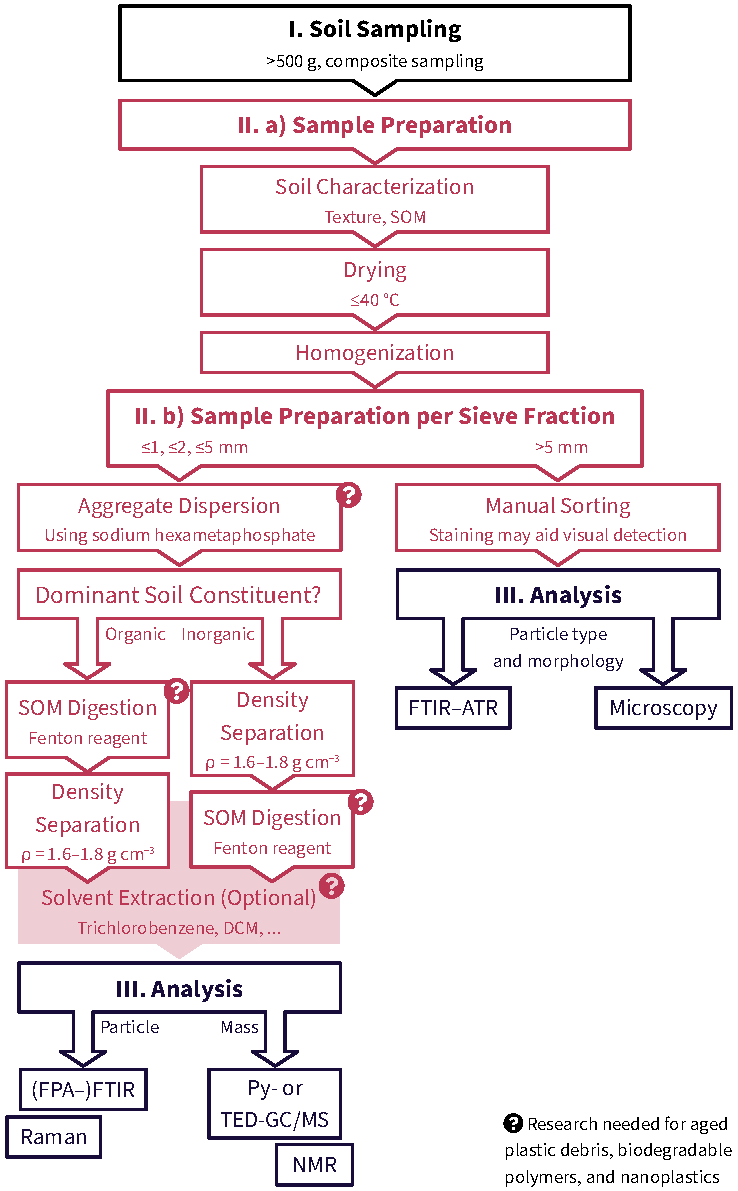
\includegraphics[width=3.28in]{figures/analytical-overview}
	\caption{Suggestions for best-practice sample preparation for microplastic analysis of soil.}
	\label{fig:analytical-overview}
	\forceversofloat
\end{figure}

Sample preparation involves drying below \SI{60}{\degreeCelsius}, ideally \SI{<=40}{\degreeCelsius}, to avoid any deterioration of microplastic particles (Section~\ref{sec:analytical-techniques:drying}). This may be particularly important for preserving biodegradable polymers. Whether freeze drying might fragment microplastics by frost wedging is unknown to date. After sufficient homogenization, soil should be sieved to \SIlist{1;2;5}{\milli\meter} to comply both with established soil texture classifications and microplastic definitions (Section~\ref{sec:analytical-techniques:homogenization}).
Further sample preparation is performed per sieve fraction. While manual sorting of macroplastics often suffices for the sieve fraction \SI{>5}{\milli\meter}, finer fractions (\SIlist{<=1;<=2;<=5}{\milli\meter}) may require dispersing soil aggregates to retrieve occluded microplastics (Section~\ref{sec:analytical-techniques:dispersion}). However, it still needs to be assessed whether soil sieving and dispersion methods like agitation with sodium hexametaphosphate solution or ultrasonication may fragment aged or biodegradable microplastics as well as nanoplastics.

If inorganic minerals are dominant in the investigated soil, the microplastic fraction should be preconcentrated by density separation
(Section~\ref{sec:analytical-techniques:density-separation}). Selecting a specific density separation setup involves careful consideration of the targeted polymers and particle sizes, recoveries, cost efficiency, ease of operation, and environmental concerns. To extract all major polymer types, aiming for determination of total plastic contents in soil, high-density solutions ($\rho$ = \SIrange{1.6}{1.8}{\gram\per\cubic\centi\meter}) such as \ch{NaBr} or \ac{spt} are recommended. Solutions with lower densities like saturated \ch{NaCl} solution may be useful for target analyses, particularly of \ac{pe}, \ac{pp}, and \ac{ps}. In any case, separation methods should be validated by recovery experiments that involve spiking known polymer types and particle sizes to a realistic, well-characterized soil matrix. In addition, potential sources of contamination need to be closely monitored, for instance, by using procedural blanks and closed containers. In this respect, separation funnels may be a promising alternative to open vessels that are currently the most common equipment for microplastic separation.

Additional \ac{som} removal (Section~\ref{sec:analytical-techniques:som-removal}) is necessary if analytical interferences from \ac{som} are expected. Ideally, \ac{som} removal agents should efficiently digest or degrade \ac{som} while preserving microplastic analytes. Current literature recommends Fenton reagent, which allows for efficient \ac{som} oxidation at controlled temperatures (\SI{<=40}{\degreeCelsius}) and thus has minimal impact on microplastics. An alternative may be selective extraction of polymers in organic solvents like \ac{dcm} or \ac{tcb} at elevated temperature (Section~\ref{sec:analytical-techniques:solvent-extraction}) while keeping interfering \ac{som} in the precipitate. By doing so, physical properties of the particles will be lost. Nonetheless, such approaches may become increasingly relevant due to the growing demand for quantitative methods for biodegradable plastics, which are more sensitive to degradation during sample preparation than conventional polymers.

The major options for subsequent microplastic analysis are visual microscopy for particles \SI{>500}{\micro\meter} (Section~\ref{sec:analytical-techniques:microscopy}), \ac{ftir} or Raman (micro)spectroscopy for smaller particles (Section~\ref{sec:analytical-techniques:spectroscopy}), mass-based thermoanalytical methods (Section \ref{sec:analytical-techniques:thermoanalysis}), and quantitative \ac{hnmr} spectroscopy (Section~\ref{sec:analytical-techniques:further-techniques}). If particle numbers, sizes, and morphology are of specific interest to the research question, spectroscopic methods are favorable. For quantifying plastic pollution in terms of mass, which has been argued to be more comparable, thermoanalytical methods and \ac{hnmr} spectroscopy may be preferred. The associated \acp{lod} in terms of microplastic size need to be stated, also taking previous sample preparation steps into account.

Terrestrial microplastics research is a quickly evolving field characterized by an extraordinarily high diversity of newly developed or refined analytical approaches. While this challenges future standardization, active method development offers great opportunities for innovations and microplastic analyses tailored to specific research questions. However, harmonization needs to start with uniform communication of microplastic quantities in particles \si{\per\kilo\gram} for microplastic counts and in \si{\micro\gram} or \si{\gram\per\kilo\gram} for mass-based results \citep{BraunMicroplastics2018}. Furthermore, quality control measures should be implemented at an early stage of method development.
This includes
\begin{enumerate*}
	\item controlling contamination by working plastic-free and including blank measurements,
	\item thorough documentation of the studied soil, sample preparation, and analytical methods, and
	\item method validation with recovery tests and an assessment of analytical limitations
\end{enumerate*}.
In this respect, the best practices for terrestrial microplastic analysis still need to be established. Because of the complexity and heterogeneity of soil, soil sample preparation for microplastic analysis must be adapted to the specific properties and composition of the examined soil.
This will not only help to ensure efficient matrix removal while conserving microplastics, it will also advance the field towards a better understanding of processes and interactions of microplastic particles with \ac{som} and other soil constituents.

% !TeX spellcheck = en_US

\chapter{Screening for Plastic Debris in Plastic-Covered Soil}
\label{ch:screening}

\paragraph{Abstract}
Agricultural plastic covers\marginnote{This chapter is based on: \fullcite{SteinmetzAre2021}.\par See \nameref{ch:author-contributions}, page~\pageref{ch:author-contributions}, for details.} made from polyethylene (\ac{pe}) and polypropylene (\ac{pp}) provide increased yields and an improved crop quality. However, such covers are suspected of partially breaking down into smaller debris and thereby contributing to soil pollution with microplastics. To scrutinize this, we randomly sampled 240 topsoil cores (\SIrange{0}{5}{\centi\meter}) from eight fields which were covered with fleeces, perforated foils, and plastic mulches for less than two years. Samples from the field periphery (\SI{50}{\meter} perimeter) served as a reference. Visual plastic debris \SI{>2}{\milli\meter} was analyzed by \ac{ftir}. Smaller, soil-associated plastic debris was dispersed from \SI{50}{\gram} of fine soil (\SI{<=2}{\milli\meter}) using sodium hexametaphosphate solution and density-separated with saturated \ch{NaCl} solution. The collected \ac{pe}, \ac{pp}, and \ac{ps} debris was selectively dissolved in a mixture of \ac{tcb} and \textit{p}-xylene at \SI{150}{\degreeCelsius} and quantified by \ac{py-gc-ms}. We counted six \ac{pe} and \ac{ps} fragments \SI{>2}{\milli\meter} in two out of eight fields. By contrast, \ac{py-gc-ms} detected \ac{pe}, \ac{pp}, and \ac{ps} contents in the fine soil of six fields (\SI{6}{\percent} of all samples). In three fields, \ac{pe} levels of \SIrange{3}{35}{\milli\gram\per\kilo\gram} were potentially associated with the use of thinner and less durable perforated foils (\SI{40}{\micro\meter} thickness). This was slightly more pronounced at field edges where the plastic covers are turned and weighted down. By contrast, \SI{50}{\micro\meter} thick \ac{pe} films were not shown to emit any plastic debris. \ac{pp} contents of \SIrange{5}{10}{\milli\gram\per\kilo\gram} were restricted to single observations in the field centers of three sites. On one site, we found expanded \ac{ps} particles \SI{>2}{\milli\meter} that concurred with elevated \ac{ps} levels (\SIrange{8}{19}{\milli\gram\per\kilo\gram}) in the fine soil. Both \ac{pp} and \ac{ps} were distributed indistinctly across sites so that their source remained unresolved. In addition, the extent to which plastic contents of up to \SI{7}{\milli\gram\per\kilo\gram} in the field periphery of some sites were attributed to wind drift from the covered fields or from external sources needs to be investigated in future studies. Our results suggest that the short-term use of thicker and more durable plastic covers should be preferred over thinner or perforated films to limit plastic emissions and accumulation in soil.

\section{Introduction}

The use of plastic covers has become common agricultural practice for improving yields and crop quality, managing harvest times, and increasing pesticide and water use efficiency \citep[Chapter~\ref{ch:plastic-mulching};][]{LamontPlastic1993}. The most used materials are \ac{pe} films and \ac{pp} fleeces of various thicknesses made to last for up to \num{10}~years \citep{BertlingKunststoffe2021}. However, wind, heavy machinery, or \ac{uv} irradiation are likely to disintegrate parts of the covers into debris smaller than \SIrange{1}{5}{\milli\meter} \citep{Scarascia-MugnozzaPlastic2011}, termed microplastics \citep{HartmannAre2019}. In recent years, this supposition has raised a discussion about agricultural plastic covers acting as a potential source of plastic debris in the terrestrial environment and particularly in soil \citep[Chapter~\ref{ch:plastic-mulching};][]{HurleyFate2018}. Yet, the actual contribution of agricultural plastic covers to soil pollution with plastic debris has remained incompletely understood and rarely discriminated from other potential sources like aerial deposition or littering.

These knowledge gaps are probably because the few studies that have analyzed plastics in and on soil so far mostly relied on optical detection by \ac{ftir} spectroscopy or visual microscopy. Both techniques deliver particle counts, are relatively sensitive to matrix interferences, and thus require extensive sample preparation when applied to heterogeneous matrices with a similar particle structure to the plastic particles of interest (Chapter~\ref{ch:analytical-techniques}). For those reasons, \citet{PiehlIdentification2018,HarmsAmount2021} excluded plastic debris \SI{<1}{\milli\meter} from their \ac{ftir} analysis of agricultural topsoil (\SIrange{0}{5}{\centi\meter}). The investigated sites were not covered with plastic, yet the soil contained \numrange[range-phrase={ to }]{0.3}{6}\,particles\,\si{\per\kilo\gram} of \SIrange{1}{5}{\milli\meter} size. These findings contrast \citet{ZhangDistribution2018} who detected \SI{95}{\percent} of plastic debris \SI{<10}{\milli\meter} (up to \num{40000}\,particles\,\si{\per\kilo\gram}) in the size fraction of \SIrange{0.05}{1}{\milli\meter} after more than \num{25}~years of permanent greenhouse cultivation. Topsoil previously covered with plastic revealed plastic counts of \numrange[range-phrase={ up to }]{60}{1000}\,particles\,\si{\per\kilo\gram} correlating with the \numrange{5}{24}~years of continuous plastic coverage \citep{HuangAgricultural2020}. \ac{pe} and \ac{pp} are typically found the most \citep{HarmsAmount2021,KimAbundance2021}. However, there are still studies which neither state particle sizes and analysis cutoffs nor assess the polymer composition of the retrieved particles \citep[for example,][]{ZhangSimple2018,BeriotLow2021}. Moreover, mass-based information is still missing but urgently needed for the monitoring and regulation of plastics in the environment.

With this study, we aimed to understand the mass distribution of plastic debris associated with fine soil (\SI{<=2}{\milli\meter}) better and to scrutinize the extent to which agricultural plastic covers emit plastic debris into their surroundings. In contrast to other studies, we screened fields covered with plastic for less than two years, which reflects typical land use and crop rotations in Germany \citep{HarmsAmount2021}.
To this end, we randomly sampled topsoil within and around eight commercially managed agricultural fields covered with fleeces, perforated foils, and plastic mulches. \ac{pe}, \ac{pp}, and \ac{ps} debris \SI{<=2}{\milli\meter} was quantified by solvent-based \ac{py-gc-ms} (Chapter~\ref{ch:py-gc-ms-method}). To better account for the heterogeneous distribution of plastic debris in soil, we further refined and validated a new sample preparation procedure involving soil aggregate dispersion and density separation that allowed for the analysis of up to \SI{50}{\gram} soil. The analyses were complemented by \ac{ftir}--\ac{atr} for plastic debris \SI{>2}{\milli\meter}.
We hypothesized that a directed gradient of plastic debris from the field center to its periphery (\SI{50}{\meter} field perimeter) supports the assumption of plastic covers contributing to an increased soil pollution with plastic debris. On the contrary, an undirected gradient would suggest another source of pollution such as littering. A uniform distribution may be an indicator for aerial deposition. In addition, we expected field margins (\SI{5}{\meter} perimeter) to be hotspots for plastic debris due to mechanical stress subjected to the plastic covers by weighting them down with soil or sandbags.

\section{Methods}

\subsection{Study Area}

The screening study was conducted in cooperation with local farmers on commercially managed horticultural fields in the Palatinate region in southwestern Germany.
The study area has a mild and dry climate with mean annual temperatures of \SIrange{10}{13}{\degreeCelsius} and a total annual precipitation of \SI{600(100)}{\milli\meter} \citep{AgrarmeteorologieRheinland-PfalzWetterdaten2020}.

Sites 1--3 were located near \foreignlanguage{ngerman}{Offenbach an der Queich}\sidenote{GPS coordinates: 49° 12' N, 8° 11' E.} and cultivated with strawberries (\textit{Fragaria\,\texttimes\,ananassa}). Site 1 was fully covered with white fleece (\SI{100}{\micro\meter} thickness) and overlain by an additional \SI{40}{\micro\meter} thick perforated foil (750\,punch holes\,\si{\per\meter\squared}) for one growing season; namely for the last four months. Site 2 had plastic-mulched ridges (black, \SI{50}{\micro\meter} thickness) and bare furrows established two years ago. On top of this, the complete field was covered with white fleece (\SI{100}{\micro\meter} thickness) for the growing season. Site 3 was mulched like site 2 but without any additional fleece cover (Figure~\ref{fig:sites}a).

Sites 4 and 5 were located near \foreignlanguage{ngerman}{Schifferstadt}\sidenote{GPS coordinates: 49° 24' N, 8° 21' E.} and cultivated with lettuce (\textit{Cichorium endivia}) and cabbage (\textit{Brassica oleracea} var. \textit{gongylodes}), respectively. Both fields were completely covered with white fleece (\SI{40}{\micro\meter} thickness) and a top layer of white perforated foil (\SI{50}{\micro\meter} thickness, \num{750}\,punch holes\,\si{\per\meter\squared}, Figure~\ref{fig:sites}b) for the growing season.

Sites 6--8 were situated in \foreignlanguage{ngerman}{Landau in der Pfalz}\sidenote{GPS coordinates: 49° 11 N, 8° 10' E.}. The rhubarb cultivation (\textit{Rheum rhabarbarum}) was fully covered with white perforated foil for the growing season. The foil on site 6 had 250\,punch holes\,\si{\per\meter\squared} and was \SI{50}{\micro\meter} thick. On site 7, the number of punch holes was similar to site 6, but the film thickness was only \SI{40}{\micro\meter}. By contrast, the foil on site 8 (\SI{40}{\micro\meter} thickness) had \num{750}\,punch holes\,\si{\per\meter\squared} (Figure~\ref{fig:sites}c).

\begin{figure*}
	\centering
	\includegraphics[width=15cm]{figures/sites}
	\caption[Exemplary photographs of the experimental sites.]{Exemplary photographs of site 3, 4, and 8 field edges covered with (a) mulch, (b) fleece and perforated foil, and (c) perforated foil, respectively.}
	\label{fig:sites}
\end{figure*}

\subsection{Sampling Strategy}

To systematically screen these agricultural fields for plastic debris, each site was subdivided into four transects as shown in Figure~\ref{fig:transects}. The field center and the inner field edge, defined as a \SI{5}{\meter} strip around the field center, were cultivated and covered with plastic film. In these transects, plant rows (ridges) and track rows (furrows) were sampled separately. The outer field margin was marked by the \SI{5}{\meter} perimeter around the cultivation. The field periphery (\SI{50}{\meter} perimeter around the cultivation) served as a reference.

Prior to retrieval of the plastic covers in spring 2018, small portions of the plastic cover were grab-sampled for subsequent characterization.
Soil samples were taken \num{<1}~week after retrieval of the plastic covers. The sampling spots were predefined by projecting a \num{1}\,\texttimes\,\SI{1}{\square\meter} grid onto each transect and randomly selecting five squares without replacement (30 per site). At each of these spots, topsoil (\SIrange{0}{5}{\centi\meter} depth) was sampled using a stainless steel core cutter (\SI{5}{\centi\meter} diameter). The soil cores were immediately transferred to uncoated paper bags and air-dried in there to reduce the risk of contamination.

\begin{figure}
	\centering
	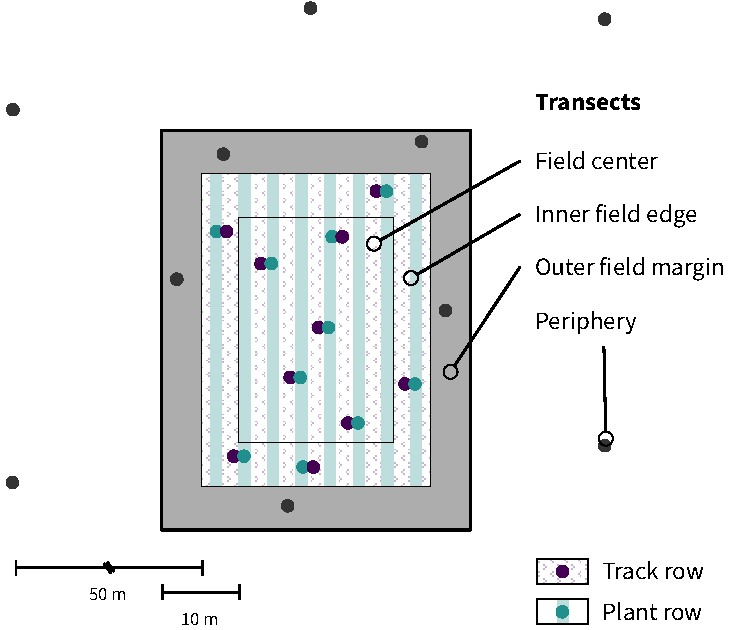
\includegraphics[width=3.267in]{figures/transects}
	\caption[Sampling scheme.]{Sampling scheme for one exemplary site; soil samples (filled dots, $n = 5$ per transect) were randomly selected. At the cultivated field centers and inner field edges, plant and track rows were sampled separately. The outer field margin and the field periphery were uncultivated.}
	\label{fig:transects}
\end{figure}

\subsection{Soil Characterization and Chemical Analysis of Plastic Covers}
\label{subsec:characterization}

The soil texture on each site was estimated from composite subsamples using the hydrometer method described in \citet{ASTMD422-63Standard2007}. The \ac{ec} and pH were measured in deionized water and \SI{0.01}{\Molar} \ch{CaCl_2} aqueous solution, respectively. Soil \ch{C} and \ch{N} were determined by dry combustion elemental analysis\sidenote{Vario MICRO Cube, Elementar, Germany.}.

The grab-sampled plastic covers were characterized by qualitative \ac{ted-gc-ms} and \ac{py-gc-ms}, \ac{dsc}, \ac{tga}, and \ac{ftir}--\ac{atr} analysis.
\ac{ted-gc-ms} and \ac{py-gc-ms} were applied to assess volatile additives or other polymer\-/associated compounds as well as the overall polymer composition of the agricultural plastic covers. To this end, a \num{1}\,\texttimes\,\SI{1}{\square\milli\meter} piece was cut out of each plastic cover and placed into a pyrolyzer quartz tube of a Pyroprobe 6150 filament pyrolyzer\sidenote{CDS Analytical, Oxford, US.} coupled with a Trace GC Ultra with DSQII \ac{ms}\sidenote{Thermo Fisher Scientific, Bremen, Germany.}.
For the \ac{ted-gc-ms} analysis, the pyrolyzer interface was flash heated (\SI{10}{\kelvin\per\milli\second}) to \SI{300}{\degreeCelsius} for \SI{15}{\second} to volatilize any polymer\-/associated compounds. A passivated transfer line (\SI{350}{\degreeCelsius}) transferred the volatiles to the \ac{ssl} injector (\SI{300}{\degreeCelsius}, split ratio 1:75) of the \ac{gc-ms} system.
The compounds were chromatographically separated in a \SI{1.3}{\milli\liter\per\minute} \ch{He} flow on a \SI{30}{\meter}\,\texttimes\,\SI{0.25}{\milli\meter} capillary column (\SI{5}{\percent} phenyl-arylene, \SI{95}{\percent} dimethylpolysiloxane, \SI{0.25}{\micro\meter} film thickness)\sidenote{ZB-5MS, Phenomenex, Aschaffenburg, Germany.}. The oven program was: \SI{40}{\degreeCelsius} (\SI{2}{\minute} hold), \SI{8}{\kelvin\per\minute} ramp to \SI{300}{\degreeCelsius} (\SI{5}{\minute} hold). The \ac{gc-ms} transfer line was kept at \SI{280}{\degreeCelsius}, and the \ac{ms} ion source (\SI{70}{\electronvolt}) was heated to \SI{230}{\degreeCelsius}. The \ac{ms} monitored \SIrange{50}{280}{\mz} at a scan rate of \SI{500}{\per\second}.
After \ac{ted-gc-ms}, the sample was pyrolyzed at \SI{750}{\degreeCelsius} for \SI{15}{\second} applying the same \ac{gc-ms} settings. All chromatograms were evaluated using OpenChrom, version 1.4.0.202103172155 \citep{WenigOpenChrom2010}, with the NIST08 database for peak identification.

\ac{dsc} and \ac{tga} measurements were conducted in accordance with Chapter~\ref{ch:tga-ms-method}. In brief, \ac{dsc} was applied between \SIrange[range-phrase={ and }]{-50}{250}{\degreeCelsius} (\SI{10}{\kelvin\per\minute} ramp, \SI{50}{\milli\liter\per\minute} \ch{N_2} flow)\sidenote{Q1000, TA Instruments, New Castle, US.} to determine the melting and crystallization temperatures of the agricultural plastic films.
For the determination of polymer degradation onsets and evolved gases, plastic samples were subjected to \ac{tga}\sidenote{STA 449 F3 Jupiter with QMS 403 C Aëolos, Netzsch, Selb, Germany.}. The heating ramp was \SI{5}{\kelvin\per\minute} from \SIrange[range-phrase={ to }]{40}{1000}{\degreeCelsius} under a \SI{20}{\milli\liter\per\minute} \ch{Ar} flow. The degradation onset was determined by the temperature at which the polymer starts to thermally decompose (\SI{<1}{\percent} mass loss).

Complementary \ac{ftir}--\ac{atr} analyses were performed between \SIrange[range-phrase={ and }]{4000}{650}{\per\centi\meter} at a resolution of \SI{4}{\per\centi\meter} using a Cary 630 spectrometer\sidenote{Agilent, Santa Clara, California, US.}. Peaks were identified with Open Specy, version 0.9.2 \citep{CowgerMicroplastic2021}.

\subsection{Soil Sample Preparation and Visual Pre-screening}
\label{sec:sample-prep}

All soil cores were sieved to fine soil (\SI{<=2}{\milli\meter}) and manually homogenized as suggested in Chapter~\ref{ch:analytical-techniques}. Visual plastic items retained by the sieve (\SI{>2}{\milli\meter}) were picked, photographed\sidenote{Leica S9i, Wetzlar, Germany.}, and analyzed via \ac{ftir}--\ac{atr} as described in the previous section.

Plastic debris \SI{<=2}{\milli\meter} were density-separated from the soil matrix using saturated \ch{NaCl} solution. To this end, \SI{50}{\gram} of fine soil were first weighted into \SI{1}{\liter} separation funnels with \ac{ptfe} stop cock\sidenote{Carl Roth, Karlsruhe, Germany.} and agitated at \SI{150}{rpm} with \SI{125}{\milli\liter} of sodium hexametaphosphate\sidenote{\cas{68915-31-1}, \SI{>=99}{\percent} purity, Carl Roth, Karlsruhe, Germany.} solution (\SI{40}{\gram\per\liter}) for \SI{2}{\hour} to disperse any soil aggregates. In a second step, \SI{90}{\gram} of \ch{NaCl}\sidenote{\cas{7647-14-5}, \SI{>=99.8}{\percent} purity, Carl Roth, Karlsruhe, Germany.} and \SI{125}{\milli\liter} of ultra-pure water were added to obtain a density solution of \SI{1.2}{\gram\per\cubic\centi\meter}. The mixture was shaken for another \SI{2}{\hour} and left for sedimentation for at least \SI{16}{\hour}. The sedimented soil was released from the separation funnel by gentle stirring of the suspension using the curved end of a bicycle spoke. Afterwards, the supernatant was collected in pleated cellulose filters with a particle retention of \SIrange{4}{12}{\micro\meter}\sidenote{Whatman 589/2, GE Healthcare, Buckinghamshire, UK.}. The filter cakes were transferred into glass culture tubes \sidenote{\num{16}\,\texttimes\,\SI{100}{\square\milli\meter}, GL18, VWR, Darmstadt Germany.} and dried at \SI{60}{\degreeCelsius}.

Based on Chapter~\ref{ch:py-gc-ms-method}, the culture tubes were topped off with \SI{8}{\milli\liter} of a 1:1-mixture (v+v) of \textit{p}-xylene\sidenote{\cas{106-42-3}, \SI{>98}{\percent} purity, Fluka Analytical, München, Germany.} and \ac{tcb}\sidenote{\cas{120-82-1}, \SI{99}{\percent} purity, Alfa Aesar, Kandel, Germany.}. In addition, the mixture contained \SI{100}{\milli\gram\per\liter} butylated hydroxytoluene\sidenote{\cas{128-37-0}, \SI{>=99}{\percent}, Merck, Darmstadt, Germany.} to prevent polymer oxidation.
The tubes were sealed with a \ac{ptfe} packing\sidenote{Carl Roth, Karlsruhe, Germany.}, vortexed, and heated at \SI{150}{\degreeCelsius} for \SI{1}{\hour} to facilitate the extraction of the polymer analytes from the filter cake.
After cooling down to room temperature, the supernatant was spiked with deuterated \ac{ps} (\ac{ps}-d5)\sidenote{PolymerSource, Quebec, Canada.} for internal standardization using positive displacement pipettes with glass capillaries\sidenote{Transferpettor micro, Brand, Wertheim, Germany.}. The extracts were stored in \SI{2}{\milli\liter} ND9 glass vials with inserts and \ac{ptfe}-sealed caps\sidenote{Wicom, Heppenheim, Germany.}.

\subsection{Quantification of Plastic Debris in Soil}

\ac{pe}, \ac{pp}, and \ac{ps} debris in fine soil (\SI{<=2}{\milli\meter}) were quantified via \ac{py-gc-ms} as detailed in Chapter~\ref{ch:py-gc-ms-method}.
In brief, \SI{2}{\micro\liter} sample aliquots were injected into pyrolyzer quartz tubes equipped with two microfiber filter discs\sidenote{Whatman QM-A, Kent, UK.} using a \SI{10}{\micro\liter} syringe with \ac{ptfe} plunger\sidenote{Hamilton 1701 N with 26s gauge, Bonaduz, Switzerland.}.
Each sample was measured once as described in Section~\ref{subsec:characterization}. However, the pyrolyzer interface was first held at \SI{300}{\degreeCelsius} to purge remaining solvents and volatiles on-line. After \SI{3}{\minute}, the sample was flash pyrolyzed (\SI{10}{\kelvin\per\milli\second}) at \SI{700}{\degreeCelsius} for \SI{15}{\second} and transferred to the \ac{gc-ms} system. The \ac{ms} selectively monitored \SIlist{70;126}{\mz} for the \ac{pp} pyrolysate 2,4-dimethyl-1-heptene (2,4Me9:1(1), \ac{ri} \num{841}), \SIlist{104;118}{\mz} for the \ac{ps} pyrolysates styrene (Sty, \ac{ri} \num{895}) and $\alpha$-methylstyrene ($\alpha$MeSty, \ac{ri} \num{981}), respectively, and \SIlist{82;95}{\mz} for \ac{pe} \textit{n}-alkadienes like 1,21-docosadiene (22:2(1,21), \ac{ri} \num{2187}). The internal standard styrene-d5 (Sty-d5, \ac{ri} \num{892}) was acquired at \SI{109}{\mz}.

\subsection{Method Validation}

The reference polymers used for external standardization and recovery experiments were analytical grade \ac{pe} beads\sidenote{\cas{9002-88-4}, \SI{500}{\micro\meter} average particle size, Alfa Aesar, Kandel, Germany.}, \ac{pp} fragments\sidenote{\cas{9003-07-0}, isotactic, \SI{<=1000}{\micro\meter}, Aldrich Chemistry, Taufkirchen, Germany.}, and \ac{ps} beads\sidenote{\cas{9003-53-6}, \SI{250}{\micro\meter} average particle size, Goodfellow, Huntingdon, UK.} (see Chapter~\ref{ch:py-gc-ms-method} for details).

The \ac{py-gc-ms} system was calibrated weekly against external standards (\SIrange{5}{200}{\micro\gram\per\milli\liter} \ac{pe}, \ac{pp}, and \ac{ps} dissolved in \textit{p}-xylene/\ac{tcb} at \SI{150}{\degreeCelsius}) following the protocol outlined in Chapter~\ref{ch:py-gc-ms-method}. Calibration curves were evaluated for signal sensitivity (slope) and linearity (adj. $R^2$). Daily sample measurements were bracketed with \SI{100}{\micro\gram\per\milli\liter} standards to correct for inter-day variations. The intra-day repeatability was determined by consecutive injections of \SI{100}{\micro\gram\per\milli\liter} standards ($n$ = 12). The internal standard \ac{ps}-d5 added after sample extraction was used for continuous repeatability checks of sample measurements.

To evaluate the plastic recovery from soil, triplicates of two agricultural reference soils were spiked at \SIlist{2;20}{\milli\gram\per\kilo\gram} of each polymer. The used reference soils were a loamy sand (\SI{8}{\percent} clay, \SI{16}{\percent} silt, \SI{76}{\percent} sand) with a \ch{C_{org}} content of \SI{1.7}{\percent} (LUFA 2.2) \sidenote{\foreignlanguage{ngerman}{Landwirtschaftliche Untersuchungs- und Forschungsanstalt, Speyer}, Germany.} and a silty clay (\SI{47}{\percent} clay, \SI{41}{\percent} silt, \SI{12}{\percent} sand) with \SI{2.5}{\percent} \ch{C_{org}} (RefeSol 06-A)\sidenote{Fraunhofer IME, Schmallenberg, Germany.}.
Instrumental and method \acp{lod} and \acp{loq} were calculated from standard deviations (\ac{sd}s) of signal intensities of low analyte concentrations (\SI{2}{\micro\gram\per\milli\liter}) and blank reference soils ($n$ = 3), respectively, in accordance with Chapter~\ref{ch:py-gc-ms-method}, \citet{DIN32645Chemical2008}, and \citet{MagnussonEurachem2014}. The selectivity against other potentially interfering non-target polymers was estimated from peak intensities of \ac{pe}, \ac{pp}, and \ac{ps} pyrolysates in LUFA 2.2 soil spiked at each \SI{40}{\milli\gram\per\kilo\gram} \ac{pet}, \ac{pmma}, \ac{pvc}, and \ac{twp}. The \ac{pet} came from a cryomilled bottle recyclate\sidenote{PETKA CZ, Brno, Czech Republic.} as detailed in Chapter~\ref{ch:tga-ms-method}. The \ac{pmma} was ground from a commercial plexiglass\sidenote{\foreignlanguage{ngerman}{Bundesanstalt für Materialforschung und -prüfung}, Berlin, Germany.}. The \ac{pvc} was purchased from Aldrich Chemistry\sidenote{Taufkirchen, Germany.}, and the \ac{twp} was from a test rig at \foreignlanguage{ngerman}{Bundesanstalt für Straßenwesen}\sidenote{Bergisch Gladbach, Germany.}.
In addition, a matrix-matched calibration was performed in LUFA 2.2 soil extracts in accordance with \citet{MagnussonEurachem2014} to assess the effect of soil matrix on the calibration parameters.

\subsection{Quality Control}

To prevent the risk of contamination, all laboratory equipment coming into direct contact with the sample or the extract solution was made of glass, metal, paper, or \ac{ptfe}. \ac{pe}, \ac{pp}, or \ac{ps} equipment was completely avoided. The worn laboratory coats were of \SI{100}{\percent} cotton. In addition, all samples and extracts were kept in closed vessels or covered with aluminum foil. The vessels were only opened under a fume hood.

The sample extraction was monitored with weekly procedural blanks that underwent the complete extraction procedure as the samples but without soil addition. Plastic contents in our procedural blanks were exclusively below the \ac{lod}.

\subsection{Data Evaluation}

Data processing and statistical analyses were conducted using R (version 4.1.0) with ``data.table'', ``magrittr'', and ``envalysis'' as main libraries. The results are given as
mean\,\textpm\,\ac{sd}. Measurement repeatabilities are stated as percentage \ac{rsd}. Matches from the Open Specy \ac{ftir} library are reported as Pearson's $r$.

The potential matrix effect on the calibration was evaluated using \ac{sse} ratios (Eq.~\ref{eq:sse}) which compare
the slope of a calibration curve prepared in solvent ($b_\mathrm{solv}$) with that of the matrix-matched calibration
($b_\mathrm{matrix}$) \citep{MagnussonEurachem2014}.

\begin{equation}
	\label{eq:sse}
	\mathrm{\ac{sse}} = \frac{b_\mathrm{matrix} - b_\mathrm{solv}}{b_\mathrm{solv}}
\end{equation}

\section{Results and Discussion}

\subsection{Soil Properties}

According to \citet{FAOWorld2014} classification, the investigated soils were identified as anthrosols. The dominant soil textures were silty clay and clayey silt (Table~\ref{tab:soils}), with sites 1, 3, and 4 showing the highest clay contents (\SI{>30}{\percent}) compared to the remaining sites. Sites 1--3 and sites 6--7 had \ch{C_{org}} contents of \SIrange{1.1}{1.3}{\percent} and \SIrange{1.4}{1.5}{\percent}, respectively. The lowest \ac{Corg} contents (\SI{0.9}{\percent}) were found on sites 4 and 5. Soil \ch{N} was \SI{<=0.2}{\percent} across all sites. The soil pH was slighly acidic (\numrange{6.6}{7.0}), and the \ac{ec} ranged from \SIrange[range-phrase={ to }]{118}{536}{\micro\siemens\per\centi\meter}. The highest \ac{ec} values were observed on sites 6 and 7.

\begin{table*}
	\centering\footnotesize
	\caption{Soil properties of experimental sites.}\label{tab:soils}
	\begin{tabular}{lllS[table-format = 2]S[table-format = 2]S[table-format = 2]lS[table-format = 1.1]S[table-format = 1.1]S[table-format = 1.1]S[table-format = 1.1]S[table-format = 3]}
		\toprule
		{Site} & {Cover (bottom to top)} & {Location} & {Clay} & {Silt} & {Sand} & {Texture\textsuperscript{\textdaggerdbl}} & {\ch{C_{org}}} & {\ch{C_{total}}} & {\ch{N_{total}}} & {pH} & {\ac{ec}} \\
		& & & {[\si{\percent}]} & {[\si{\percent}]} & {[\si{\percent}]} & & {[\si{\percent}]} & {[\si{\percent}]} & {[\si{\percent}]} &  & {[\si{\micro\siemens\per\centi\meter}]} \\
		\midrule
		1 & Fleece (\ac{pp}), perforated foil (\ac{pe}) & Offenbach & 34 & 53 & 13 & Tu3 & 1.3 & 1.3 & 0.1 & 6.6 & 200 \\
		2 & Mulch (\ac{pe}), fleece (\ac{pp}) & Offenbach & 10 & 77 & 13 & Ut2 & 1.1 & 1.3 & 0.1 & 6.8 & 138 \\
		3 & Mulch (\ac{pe}) & Offenbach & 36 & 64 & 0 & Tu3 & 1.2 & 1.4 & 0.1 & 6.8 & 147 \\
		4 & Fleece (\ac{pe}), perforated foil (\ac{pe}) & Schifferstadt & 32 & 67 & 1 & Tu4 & 0.9 & 1.1 & 0.1 & 6.7 & 118 \\
		5 & Fleece (\ac{pe}), perforated foil (\ac{pe}) & Schifferstadt & 24 & 76 & 0 & Ut4 & 0.9 & 1.1 & 0.1 & 6.9 & 236 \\
		6 & Perforated foil (\ac{pe}) & Landau & 25 & 75 & 0 & Ut4 & 1.4 & 1.6 & 0.2 & 6.8 & 510 \\
		7 & Perforated foil (\ac{pe}) & Landau & 21 & 79 & 0 & Ut4 & 1.5 & 1.6 & 0.2 & 6.9 & 536 \\
		8 & Perforated foil (\ac{pe}) & Landau & 15 & 85 & 0 & Ut3 & 1.4 & 1.6 & 0.2 & 7.0 & 289 \\
		\bottomrule
		\multicolumn{12}{p{.9\textwidth}}{\textsuperscript{\textdaggerdbl} In accordance with \citet{SponagelBodenkundliche2005}; Tu = silty clay, Ut = clayey silt.} \\~
	\end{tabular}
\end{table*}

\subsection{Agricultural Plastic Covers}

The fleeces that covered sites 1 and 2 were identified as \ac{pp} as indicated by multiple \ch{C-H} stretch deformations at \SIrange{2950}{2838}{\per\centi\meter} as well as \ch{CH_2} and \ch{CH_3} bends at \SIlist{1455;1377}{\per\centi\meter}, respectively (Open Specy \ac{ftir} library match: $r \geq$ \num{0.96}, see Figure~\ref{fig:ftir-covers}a for an exemplary \ac{ftir} spectrum). A shapeless broad peak between \SIrange[range-phrase={ and }]{1860}{1660}{\per\centi\meter} indicated the presence of carbonyl groups \citep{GrauseChanges2020}. The indistinct band between \SIrange[range-phrase={ and }]{1200}{900}{\per\centi\meter} may be attributed to \ch{C-O} stretching in alcohols, acids, or ethers originating from a contamination with \ac{som} or plastic aging \citep{FuMechanism2021}. Complementary \ac{dsc} showed crystallization temperatures at \SIlist{114;116}{\degreeCelsius} and melting temperatures at \SIlist{158;160}{\degreeCelsius}. Between \SIrange[range-phrase={ and }]{381}{400}{\degreeCelsius}, the polymers started to decompose into methylalkenes characteristic for \ac{pp} \citep[Figure~\ref{fig:py-covers}a for an exemplary pyrogram]{TsugePyrolysis2011}.

By contrast, the fleece from sites 4 and 5 was made of \ac{pe} ($r$ = \num{0.96}). The respective \ac{ftir} spectrum showed indicative \ch{CH_2} stretching between \SIrange{2919}{2915}{\per\centi\meter} (asymmetric)
and \SIrange{2851}{2845}{\per\centi\meter} (symmetric, Figure~\ref{fig:ftir-covers}c). The crystallization and melting temperatures were \SIlist{96;108}{\degreeCelsius}, respectively. The degradation onset was \SI{408}{\degreeCelsius} and triggered the formation of \ac{pe}-specific triplets of $n$-alkadienes, $n$-alkenes, and $n$-alkanes (Figure~\ref{fig:py-covers}c).
All other covers, namely mulches and perforated foils from sites 2--8, were made of \ac{pe} ($r \geq$ 0.86, Figure~\ref{fig:ftir-covers}b,d,e). The carbonyl band at \SIrange{1860}{1660}{\per\centi\meter} was visible in all samples but was most pronounced for the \ac{pe} mulch from sites 2 and 3. However, crystallization temperatures (\SIrange{100}{113}{\degreeCelsius}) and melting temperatures (\SIrange{110}{122}{\degreeCelsius}) of the \ac{pe} mulch were slightly higher than those of the \ac{pe} fleece. The degradation onsets of the mulches and perforated foils ranged from \SIrange[range-phrase={ to }]{384}{397}{\degreeCelsius}.

The qualitative analyses of volatile polymer additives and other polymer\-/associated compounds thermally desorbing from the agricultural films at \SI{300}{\degreeCelsius} revealed three omnipresent substances (NIST08 matches \SI{>75}{\percent}, see Figure~\ref{fig:ms-covers}): These were propyl dodecanoate\sidenote{\cas{3681-78-5} or \cas{10233-13-3}.}, oleonitrile\sidenote{\cas{112-91-4}.}, and 9-octadecenamide\sidenote{\cas{301-02-0}.} (see Figure~\ref{fig:py-covers} for exemplary chromatograms). In addition, the \ac{pp} fleeces from sites 1 and 2 as well as the \ac{pe} perforated foils from sites 4--8 contained traces of a di-\textit{tert}-butylphenol\sidenote{For instance \cas{96-79-4}.} which is an indicator for antioxidants \citep{HahladakisOverview2018}. Propyl dodecanoate and oleonitrile are lubricants probably added to agricultural plastic covers for easier spreading out on site. 9-Octadecenamide is a known degradation product of hindered amine light stabilizers like Chimassorb 944 \citep{HaiderLoss2001}. No pesticides were detected in the plastic covers, probably due to the limited sensitivity of the qualitative analysis and/or their low thermal stability.

Complementary \ac{ftir}--\ac{atr} and \ac{py-gc-ms} confirmed that both plastic mulches and perforated foils were exclusively made of \ac{pe}. The fleeces were of \ac{pe} and \ac{pp}, although \ac{pp} is more common \citep{HamouzInfluence2011}. All \ac{pe} covers melted within the range of \SIrange{109}{125}{\degreeCelsius} and degraded \SI{>318}{\degreeCelsius} as expected for virgin low-density \ac{pe} \citep{BeylerThermal2002}. Interestingly though, melting temperatures of the \ac{pp} fleeces were \SIrange[range-phrase={ to }]{5}{10}{\degreeCelsius} lower than those of virgin \ac{pp} (\SIrange{165}{170}{\degreeCelsius}) \citep{BeylerThermal2002,TochacekPolymer2019}. The degradation onset was not affected by this and comparable to virgin \ac{pp} (\SI{>315}{\degreeCelsius}) \citep{BeylerThermal2002}. Decreasing melting temperatures may indicate the presence of additives or other impurities but could also be a first sign of polymer aging as similarly observed after \numrange{5}{20} months of temperate weathering \citep{TochacekPolymer2019}. This is consistent with the carbonyl groups identified via \ac{ftir} which are indicative for the photo-oxidation of polyolefins \citep{GrauseChanges2020}. In our study, fleeces and perforated foils were on the fields for about four months. The mulches were applied two years previously. The incipient aging concurred with the release of antioxidant di-\textit{tert}-butylphenol from the \ac{pp} backbone as indicated by \ac{ted-gc-ms}. As di-\textit{tert}-butylphenol was also released from \ac{pe} perforated foils, it remains unresolved whether the presence of di-\textit{tert}-butylphenol was material-specific or indeed triggered by polymer aging.

\subsection{Visual Plastic Items on Site}

We visually identified 30 suspect items (\SI{>2}{\milli\meter}) during soil sieving. Subsequent \ac{ftir}--\ac{atr} analysis revealed six items as plastics. These were a black \ac{pe} film ($r$ = 0.92, Figure~\ref{fig:visual-items}a) and four \ac{ps} fragments ($r \geq$ 0.91, Figure~\ref{fig:visual-items}b) at the field center of site 5 (see Figure~\ref{fig:ftir-debris} for the respective \ac{ftir} spectra). The \ac{ps} showed characteristic peaks at \SIlist{3024;1492;694}{\per\centi\meter} originating from aromatic \ch{C-H} stretch and bend deformations. In the field center of site 6, a green \ac{pe} film ($r$ = 0.92, Figure~\ref{fig:visual-items}c) was found. All other items were of natural origin including invertebrate shells, stones or wood fragments, and cellulose fibers that were identified by Open Specy as chitin, resin dispersion, and cotton, respectively ($r \geq$ 0.82, Figure~\ref{fig:visual-items}d--f).

\begin{figure*}
	\centering
	\includegraphics[width=12cm]{figures/visual-items}
	\caption[Exemplary photographs of suspect particles \SI{>2}{\milli\meter}.]{(a) \ac{pe} film and (b) \ac{ps} fragment from the field center of site 5, (c) \ac{pe} film and (d) chitin shell from the field center of site 6, and (e) resin or natural fragment and (f) cotton fiber from the field edge of site 7; see Figure~\protect\ref{fig:ftir-debris} for the respective \ac{ftir} spectra.}
	\label{fig:visual-items}
\end{figure*}

In this respect, it is important to note that the visual identification of suspect items largely depends on the operator's experience and may thus lead to excessive over- or underestimation of particle numbers (Chapter~\ref{ch:analytical-techniques}). Furthermore, counting suspect items \SI{>2}{\milli\meter} in a \SI{100}{\cubic\centi\meter} soil core is hardly representative. We thus refrained from extrapolating our findings to particles\,\si{\per\kilo\gram} and intended visual identification to serve as a qualitative complement to subsequent \ac{py-gc-ms} quantification.
Interestingly though, the plastic debris \SI{>2}{\milli\meter} were exclusively found on sites 5 and 6. None of the black and green \ac{pe} or white \ac{ps} fragments matched the applied white \ac{pe} fleece and perforated foil in color or polymer type. This suggests an external source of plastic debris, for instance from adjacent streets or other fields, or residues from previous land use \citep{HarmsAmount2021}.

\subsection{\ac{py-gc-ms} Method Performance}

The pyrolysates chosen for quantifying \ac{pe}, \ac{pp}, and \ac{ps} were 22:2(1,21), 2,4Me9:1(1), and Sty, respectively, as they performed the best in terms of signal linearity (adj. $R^2 >$ \num{0.995}), instrumental \acp{lod} (\SI{<10}{\nano\gram}), and measurement repeatability (\ac{rsd} \SI{<10}{\percent}, Table~\ref{tab:py-instrument}). The $n$-alkadiene 22:2(1,21) was preferred over the respective $n$-alkene or $n$-alkane because of its higher selectivity for \ac{pe} (Chapter~\ref{ch:py-gc-ms-method}). LUFA 2.2 exerted a negligible matrix effect of \SIlist{16;-3;-2}{\percent} \ac{sse} on the selected \ac{pe}, \ac{pp}, and \ac{ps} pyrolysates (see Figure~\ref{fig:matrix-match} for calibration curves). Method \acp{lod} were \SIrange{0.7}{1.2}{\milli\gram\per\kilo\gram} in RefeSol 06-A and \SIrange{1.9}{3.3}{\milli\gram\per\kilo\gram} in LUFA 2.2. The respective method \acp{loq} ranged from \SIrange[range-phrase={ to }]{2.5}{9.5}{\milli\gram\per\kilo\gram} (Table~\ref{tab:py-validation}). A LUFA 2.2 soil containing each \SI{40}{\milli\gram\per\kilo\gram} of potentially interfering, non-target \ac{pet}, \ac{pmma}, \ac{pvc}, and \ac{twp} did not induce significant false positive detections of \ac{pe}, \ac{pp}, or \ac{ps}.

\begin{table}
	\centering\footnotesize
	\caption{Instrumental validity criteria of the \ac{py-gc-ms} method.}\label{tab:py-instrument}
	\begin{tabular}{llS[table-format = 1.4]S[table-format = 2.1]S[table-format = 2.1]}
		\toprule
		{Polymer} & {Pyrolysate} & {adj. $R^2$} & {\ac{lod}\textsuperscript{\textasteriskcentered}} & {\ac{rsd}} \\
		& & & {[\si{\nano\gram}]} & {[\si{\percent}]} \\
		\midrule
		\ac{pe} & 17:2(1,16) & 0.9912 & 9.0 & 11.3 \\
		& 18:2(1,17) & 0.9785 & 9.2 & 9.8 \\
		& 19:2(1,18) & 0.9965 & 5.6 & 11.3 \\
		& 20:2(1,19) & 0.9788 & 6.4 & 11.9 \\
		& 21:2(1,20) & 0.9897 & 10.0 & 12.8 \\
		& 22:2(1,21) & 0.9952 & 5.8 & 9.5 \\
		& 23:2(1,22) & 0.9709 & 7.2 & 11.2 \\
		\ac{pp} & 2,4Me9:1(1) & 0.9997 & 4.6 & 8.9 \\
		\ac{ps} & Sty & 0.9980 & 6.6 & 3.5 \\
		& $\alpha$MeSty & 0.9866 & 19.4 & 11.5 \\
		\bottomrule
		\multicolumn{5}{p{.55\textwidth}}{\textsuperscript{\textasteriskcentered} Instrumental limit of detection; \ac{rsd} = relative standard deviation.}
	\end{tabular}
\end{table}

\begin{table*}
	\centering\footnotesize
	\caption{Validation criteria of the extraction method.}\label{tab:py-validation}
	\begin{tabular}{llS[table-format = 1.1]S[table-format = 1.1]S[table-format = 1.1(1)]S[table-format = 3(2)]S[table-format = 3(2)]}
		\toprule
		{Polymer} & {Pyrolysate} & {\ac{lod}\textsuperscript{\textasteriskcentered}} & {\ac{loq}\textsuperscript{\textasteriskcentered}} & {Interference\textsuperscript{\textdagger}} & \multicolumn{2}{c}{Recovery} \\
		\cmidrule(lr){6-7}
		& & {[\si{\milli\gram\per\kilo\gram}]} & {[\si{\milli\gram\per\kilo\gram}]} & {[\si{\milli\gram\per\kilo\gram}]} & {at \SI{2}{\milli\gram\per\kilo\gram} [\si{\percent}]} & {at \SI{20}{\milli\gram\per\kilo\gram} [\si{\percent}]}\\
		\midrule
		\multicolumn{6}{l}{\textit{LUFA 2.2}} \\
		\ac{pe} & 22:2(1,21) & 1.9 & 9.5 &  0.9(3) & 133(9) & 105(3) \\
		\ac{pp} & 2,4Me9:1(1) & 2.9 & 2.9 & 0(0) & 70(10) & 93(5) \\
		\ac{ps} & Sty & 3.3 & 6.2 & 0(0) & 52(2) & 86(4) \\
		\multicolumn{6}{l}{\textit{RefeSoil 06-A}} \\
		\ac{pe} & 22:2(1,21) & 1.2 & 9.5 & & 30(20) & 50(10) \\
		\ac{pp} & 2,4Me9:1(1) & 0.8 & 2.5 & & 30(20) & 62(1) \\
		\ac{ps} & Sty & 0.7 & 6.2 & & 0(0) & 12(5) \\
		\bottomrule
		\multicolumn{7}{l}{\textsuperscript{\textasteriskcentered} Method limits of detection and quantification; \textsuperscript{\textdagger} introduced from \SI{40}{\milli\gram\per\kilo\gram} non-target polymers.} \\~
	\end{tabular}
\end{table*}

The extraction of \SI{20}{\milli\gram\per\kilo\gram} plastic debris from LUFA 2.2 soil yielded recoveries of \SIrange{86}{105}{\percent} (Table~\ref{tab:py-validation}). \ac{pe} was recovered the best whereas \ac{ps} showed the lowest value. Recovering plastic debris at levels close to the method \ac{lod} (\SI{2}{\milli\gram\per\kilo\gram}) and below the respective method \acp{loq} led to an overestimation of recovered \ac{pe} (\SI{133(9)}{\percent}) while underestimating \ac{pp} (\SI{70}{\percent}) and \ac{ps} (\SI{50}{\percent}). Recoveries from RefeSol 06-A were generally lower: Whereas we still recovered \SIlist{50;62}{\percent} of the \SI{20}{\milli\gram\per\kilo\gram} \ac{pe} and \ac{pp}, respectively, recoveries dropped to \SI{30(20)}{\percent} at the lower spiking level. Hardly any \ac{ps} was recovered from RefeSol 06-A (\SI{<12}{\percent}) irrespective of the spiking level.

As reviewed in Chapter~\ref{ch:analytical-techniques}, several studies have already evaluated their extraction procedures for various plastic debris from solid matrices using organic solvents like \ac{dcm} or \ac{thf}. In combination with quantitative \ac{py-gc-ms}, however, matrix interferences and false positive detections from organic matrix constituents or other non-target polymers should be closely monitored (\citealp{DierkesQuantification2019}; Chapter~\ref{ch:py-gc-ms-method}).
By combining density separation and solvent extraction with \textit{p}-xylene/\ac{tcb}, we obtained method \acp{lod} from blank LUFA 2.2 and RefeSol 06-A and interferences from non-target polymers equivalent \SI{<3.3}{\milli\gram\per\kilo\gram} \ac{pe}, \ac{pp}, and \ac{ps}, which highlights the selectivity of our method. Dispersing soil aggregates with sodium hexametaphosphate prior to density separation further enabled the quantification of plastic debris potentially occluded in or masked by soil aggregates. The required filtration step, however, systematically excluded particles \SI{<4}{\micro\meter} that were not retained by the applied filter.

Inconsistent recoveries at a spiking level below the method \acp{loq} of \SIrange[range-phrase={ to }]{2.5}{9.5}{\milli\gram\per\kilo\gram} challenged the sensitivity and robustness of our solvent-based approach. This particularly applied to the \SI{<30}{\percent} \ac{pe}, \ac{pp}, and \ac{ps} we recovered from RefeSol 06-A. While this clearly defines the quantitative limits of the method, our working range is still \numrange{10}{100} times lower than that of previous applications involving solvent-based \ac{py-gc-ms}. \Citet{DierkesQuantification2019,OkoffoIdentification2020}, for instance, spiked \SI{1}{\gram} of quartz sand and biosolids at \SIrange{0.05}{50}{\gram\per\kilo\gram} of various polymers to evaluate their accelerated solvent extraction with \ac{thf} and \ac{dcm}, respectively.
Irrespective of the spiking level though, our \ac{ps} recoveries from the clayey RefeSol 06-A were particularly low (\SI{<12}{\percent}). This is in line with \citet{WangPoor2018} who found comparable recoveries after density separation of nano-sized \ac{ps} from a silt soil. \citet{LuoDistribution2020,WuTransport2020} reasoned that \ac{som} as well as \ch{Fe} and \ch{Al} oxides effectively retain \ac{ps} particles in soil. The dramatic decrease in \ac{ps} recovery may be attributed to interactions forming between the delocalized $\pi$-electrons of the aromatic \ac{ps} ring and \ac{som}, iron and aluminum oxides, or cations bound to the negatively charged surface of clay particles \citep{NewcombDeveloping2017}. During the density separation, the aggregated \ac{ps} may have been preferentially sedimented, and thereby systematically excluded from subsequent solvent extraction. The addition of an anionic surfactant like sodium dodecyl sulfate or nonionic polysorbates during soil aggregate dispersion and density separation could counteract this, but potentially at the expense of introducing another source of \ac{pe} contamination from the surfactants' $n$-alkane domains.

Based on the two reference soils tested and on previous work (Chapter~\ref{ch:py-gc-ms-method}), we considered our method sufficiently sensitive and quantitative for environmentally-relevant \ac{pe} and \ac{pp} levels exceeding the respective method \acp{loq}. The \SI{50}{\percent} \ac{pe} and \SI{62}{\percent} \ac{pp} we recovered from RefeSol 06-A suggest a rather semi-quantitative evaluation of soils with a clay content \SI{>47}{\percent} and a \ch{C_{org}} content \SI{>2.5}{\percent}. \ac{ps} is evaluated qualitatively for its low recoveries.
These findings once more highlight the importance of specifically testing and evaluating analytical methods for plastic analysis with various soil types (Chapter~\ref{ch:analytical-techniques}). The extrapolation of specific validity criteria to field samples with a different texture and \ch{C_{org}} composition thus remains difficult and requires careful interpretation.

\subsection{\ac{pe}, \ac{pp}, and \ac{ps} Debris in Soil}

We detected plastic debris \SI{<=2}{\milli\meter} exceeding the average method \ac{lod} of \SIrange{1.5}{2.0}{\milli\gram\per\kilo\gram} in 15 out of 240 samples from six sites (Figure~\ref{fig:py-screening}). This is equivalent to \SI{6}{\percent} positive detections. Soil from sites 1, 7, and 8 contained the most \ac{pe} (10 findings) with single detections peaking at \SIlist{19;35}{\milli\gram\per\kilo\gram}. Mean \ac{pe} contents were the highest at the field margin of site 1 (\SI{10(10)}{\milli\gram\per\kilo\gram}) and decreased below the method \ac{lod} in the field edge and the field periphery. Furthermore, \ac{pe} contents were slightly higher in the track rows (furrows) than in the plant rows (ridges) of the field centers and edges of site 1. With \SIrange{4}{7}{\milli\gram\per\kilo\gram}, sites 7 and 8 showed maximum \ac{pe} contents in the field periphery. Field centers, edges, and margins contained less than \SI{2}{\milli\gram\per\kilo\gram} \ac{pe}. On these sites, differences in the \ac{pe} contents between field track and plant rows were mostly indistinct. Sites 2--6 did not contain any \ac{pe} above the method \ac{lod}.
The \ac{pp} findings were driven by single observations of \SIrange{5}{10}{\milli\gram\per\kilo\gram} in the field centers of sites 2, 4, and 7.
\ac{ps} was identified twice, namely in the periphery of sites 4 and 5. Due to the poor \ac{ps} recoveries, these findings are most likely underestimated.

\begin{figure*}
	\centering
	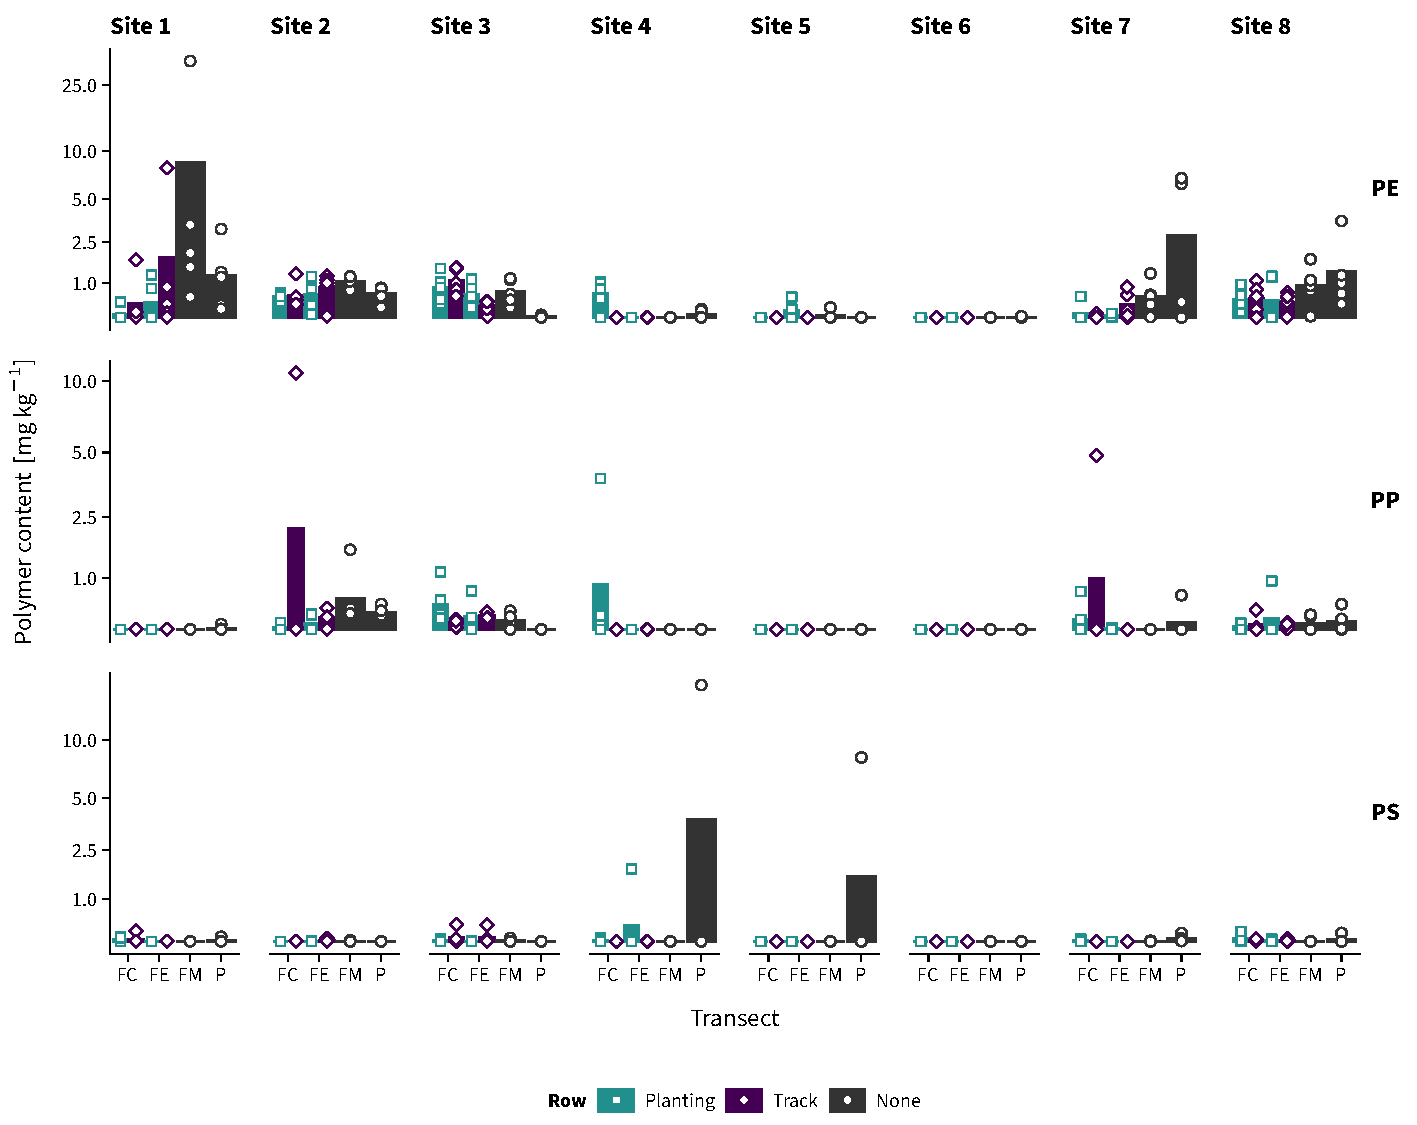
\includegraphics[width=\textwidth]{figures/py-screening}
	\caption[\Ac{pe}, \ac{pp}, and \ac{ps} contents (\SI{<=2}{\milli\meter}).]{Log-scaled \ac{pe}, \ac{pp}, and \ac{ps} contents (\SI{<=2}{\milli\meter}) at the field center (FC), field edge (FE), field margin (FM), and the periphery (P) of sites 1--8; dots represent single measurements, the underlying bar plot shows the transect average.}
	\label{fig:py-screening}
\end{figure*}

Interestingly, elevated \ac{pe} contents occurred mostly on sites 1, 7, and 8 which were covered with \SI{40}{\micro\meter} thick perforated foils. Sites 4--6 covered with thicker mulch films or perforated foils (\SI{50}{\micro\meter}) did not show any significant \ac{pe} contamination.
On the one hand, this is remarkable because the agricultural films were on site for four months only. On the other hand, the elevated plastic contents may have originated from another, potentially diffuse input source prior to plastic coverage.

Our results are yet in line with \citet{ZhangStatus2016} who attributed elevated plastic emissions to the use of particularly thin agricultural films. In China, for instance, common film thicknesses are \SIrange{6}{10}{\micro\meter}, while EU regulations stipulate agricultural covers thicker than \SI{20}{\micro\meter} \citep{EN13655Plastics2018}. This may also explain why studies conducted in non-EU countries often report extraordinarily high plastic levels in soil \citep{LiuWhite2014}, particularly after long-term use of agricultural plastics \citep{HuangAgricultural2020,ZhangDistribution2018}.

Regardless of the film thickness, the increased \ac{pe} contents at the field margin of site 1 suggested that the mechanical stress of weighing the plastic covers down with soil or digging them in favored the local formation of plastic debris. The close contact with soil and exposure to sunlight may have accelerated polymer aging and embrittlement as indicated by our complementary \ac{dsc} and \ac{ftir}--\ac{atr} measurements.
Due to the limited number of \ac{pe} detections above method \ac{lod}, we did not find a clear indication for the further translocation of plastic debris from the ridged plant rows to lower ground furrows. Tracing experiments by \citet{LaermannsTracing2021}, however, recently confirmed that the micro- and macrorelief of the soil surface may indeed favor the water erosion of plastic debris on a meter scale.
Even at larger scales though, it remained unresolved to what extent the \ac{pe} debris in the field periphery (mainly sites 7 and 8) originated from the covered field centers or whether it came from an external source via wind drift. Due to ubiquity of products made from \ac{pe}, such an external source cannot be excluded.

Although sites 1 and 2 were both fleeced with \ac{pp}, only site 2 showed elevated \ac{pp} contents. At the same time, \ac{pp} was found on sites covered exclusively with \ac{pe} for the last four months. Therefore, no clear association between \ac{pp} detections and the seasonal use of plastic covers was established. This is striking because the fibrous structure of the \ac{pp} fleece together with the initial signs of aging detected via \ac{dsc} and \ac{ftir}--\ac{atr} made emissions of plastic debris particularly likely.
Unexpectedly, these two study sites were thus most likely dominated by external sources like littering or previous land use rather than receiving plastic debris from the in situ fragmentation of fleeces.

This similarly applied to \ac{ps}, which is not used for agricultural plastic covers \citep{BertlingKunststoffe2021}, and may thus serve as an indicator for external sources of plastic debris in soil. Another possible explanation for the \ac{ps} findings on the two neighboring sites 4 and 5 may be a legacy contamination with \ac{ps}. In the past, beads made from expanded \ac{ps} were used for the conditioning and stabilization of horticultural soils \citep{MaghchicheUse2010}. However, it remained unresolved whether this was the case in the agricultural area investigated in this study.

Given that our investigated soils had a clay content of \SIrange{15}{36}{\percent}, the obtained \ac{pe}, \ac{pp}, and \ac{ps} contents were potentially
underestimated by a factor of \numrange{1.5}{2}. Even though taking this uncertainty into account, the plastic contents detected in our study were still up to \num{100} times lower than the \SI{820}{\milli\gram\per\kilo\gram} \ac{pe}, \SI{40}{\milli\gram\per\kilo\gram} \ac{pp}, and \SI{56}{\milli\gram\per\kilo\gram} \ac{ps} that \citet{DierkesQuantification2019} obtained from a non-characterized roadside soil using a comparable solvent-based \ac{py-gc-ms} method. A recent modeling study by \citet{BrandesIdentifying2021} estimated that plastic debris emitted from agricultural plastic covers may increase the plastic contents in agricultural soil by \SIrange{5}{9}{\milli\gram\per\kilo\gram} per year. By contrast, conversions from particle counts and shapes to plastic masses resulted in  contents of \SIrange{0.1}{1.2}{\milli\gram\per\kilo\gram} in agricultural soil covered with plastics \citep{BuksGlobal2020}. However, such conversions are increasingly discouraged for their high estimate errors \citep[Chapter~\ref{ch:analytical-techniques};][]{PrimpkeComparison2020}.
All this challenges comparisons since studies investigating plastic debris in agricultural soil so far exclusively used particle-based microspectroscropic techniques. Nonetheless, our results are approximately in the same order of magnitude than previous findings but should be further corroborated.

\section{Conclusions}

The combination of soil aggregate dispersion and density separation with solvent-based \ac{py-gc-ms} enabled the simple, yet selective quantification of \ac{pe} and \ac{pp} debris in agricultural soil. Analyzing a sample amount of \SI{50}{\gram} better accounted for the heterogeneous distribution of discrete plastic particles in the soil matrix. The additional dispersion step further made plastic debris occluded in soil aggregates amenable to quantification. By contrast, poor \ac{ps} recoveries potentially induced by that additional separation step challenged a reliable \ac{ps} quantification.

We applied the new method to soil randomly sampled from four predefined transects located in and around eight agricultural field covered with plastic films. This screening approach revealed first insights into the potential contribution of agricultural plastic covers to plastic pollution in soil: While \ac{pp} fleeces and \SI{50}{\micro\meter} thick \ac{pe} films were not shown to emit plastic debris into their surrounding during their use, four months of covering with thinner perforated \ac{pe} foils (\SI{40}{\micro\meter} thickness) was associated with elevated \ac{pe} contents in and around the covered fields. Due to the ubiquitous use of plastic covers and potentially interfering external plastic sources, a causal relationship between the use of plastic covers and elevated plastic levels in soil needs yet to be shown, for instance, by conducting more controlled and systematic experiments.

The maximum plastic levels were \SI{35}{\milli\gram\per\kilo\gram} and with that about 30 times higher than those previously reported for covered agricultural soil \citep{BuksGlobal2020} but several orders of magnitude lower than in a roadside soil \citep{DierkesQuantification2019}. This could mean that current EU regulations \citep{EN13655Plastics2018} and recycling efforts for agricultural plastics start to take effect but should be further intensified. The long-term use of thin perforated foils, in particular, is likely to contribute to the accumulation and further distribution of plastics in the environment. The use of thicker and more durable plastic covers may be preferred to prevent this.

To scrutinize this, future research should aim for the continuous monitoring of plastic contents in soil. This may also include samplings of deeper soil and more sensitive screenings of polymer-associated compounds including additives and agrochemicals sorbed to the plastic covers.
Advancing the field of mass spectrometric methods for the quantification of plastic debris in heterogeneous matrices will help to bridge the gap between modeling and monitoring, further the science-based regulation of agricultural plastic products, and contribute to their sustainable use.

% !TeX spellcheck = en_US

\chapter{Final Discussion and Outlook}
\label{ch:general-discussion}

\section{Thermoanalytical Approaches for the Quantification of Plastics in Soil}
\label{sec:general-discussion:analytics}

Mass-based information on the level of plastic pollution in soil is essential to link exposure data with modeling and effect data. Up to now, such data has remained largely missing for the lack of appropriate analytical methods. This has emphasized the need for further advances in analytical techniques for the mass-based quantification of plastic debris, particularly in heterogeneous samples like soil (Chapters~\ref{ch:plastic-mulching} and \ref{ch:analytical-techniques}).

A first proof-of-principle study using \ac{pet} as a model (Chapter~\ref{ch:tga-ms-method}) demonstrated the potential of thermoanalytics for the mass-based plastic quantification in soil. The taken \ac{tga-ms} approach permitted the direct analysis of ground soil. This reduced sample preparation to a minimum and thus considerably sped up analysis times with regard to microspectroscopic methods. Microspectroscopic methods normally require an extensive sample preparation including multiple separation, cleanup, and filtration steps (\citealp[for instance,][]{LoderEnzymatic2017}; Chapter~\ref{ch:analytical-techniques}). But the \ac{tga-ms} also involved certain limitations:
\begin{enumerate*}
	\item Sample amounts of about \SI{50}{\milli\gram} hindered the preparation of a representative sample prior to analysis,
	\item the \ac{ms} only detected \ac{pet} contents \SI{>0.7}{\gram\per\kilo\gram}, and
	\item the absence of chromatographic separation potentially limited the simultaneous analysis of different polymers or polymer mixtures with overlapping degradation temperatures (Table~\ref{tab:polymer-decomposition})
\end{enumerate*}.
In the further course of the project, the participation in a round robin test revealed that the developed \ac{tga-ms} method was particularly suitable for distinguishing aromatic polymers like \ac{ps} and \ac{pet} from aliphatic ones such as \ac{pe} and \ac{pp} \citep{BeckerQuantification2020}. The sum of aliphatic and aromatic polymers was each quantified accurately. Such a rough classification may suffice for simple prescreenings that aim at the identification of distinct plastic hotspots.
Chemometric analyses of \ac{tga-ms} data, for instance, using \ac{pca} and principal component regression may help to pursue a rapid identification and quantification of polymer mixtures by linking \ac{tga} and \ac{ms} data better or by deconvolving interfering signals from other polymers and soil matrix \citep{DavidIntroducing2019}. But this certainly requires further research, which is in line with \citet{MansaThermogravimetric2021} who reasoned that \ac{tga}-based methods are still underutilized for the complexity of the generated data but may provide a robust screening tool for future plastic analyses. However, advances in \ac{tga-ms} data analysis will most likely help measurement selectivity more than measurement sensitivity since the latter is physically restricted by the used \ac{ms}.

Using \ac{py-gc-ms} instead allowed for the chromatographic separation of polymer analytes after pyrolysis and their selective quantification, as recently acknowledged by \citet{Jimenez-SkrzypekCurrent2021}. The key to the method developed in Chapter~\ref{ch:py-gc-ms-method} was the use of \ac{tcb} to selectively dissolve the target analytes \ac{pe}, \ac{pp}, and \ac{ps} prior to quantification. Solvent-based \ac{py-gc-ms} not only facilitated the preparation of dilution series and sample aliquots but also the extraction of the polymer analytes from the soil matrix. Thereby, up to \SI{4}{\gram} of soil sample were analyzed while decreasing method \acp{lod} to \SIrange{1}{86}{\milli\gram\per\kilo\gram}.
At such low plastic contents though, the method became sensitive to interferences from the soil matrix (Chapter~\ref{ch:intro}). The interferences most likely originated from polymeric \ac{som} fractions that were co-dissolved with the polymer analytes. These polymeric \ac{som} fractions particularly interfered with the quantification of \ac{pe} at levels \SI{<50}{\milli\gram\per\kilo\gram}. \Citet{DierkesQuantification2019} observed similar interferences using \iac{ase}-based \ac{py-gc-ms} approach.

Since this problem could not be tackled from a mere instrumental perspective, the outcome of Chapter~\ref{ch:py-gc-ms-method} involved a critical (re-)evaluation of existing sample preparation and analytical techniques for soil samples (Chapter~\ref{ch:analytical-techniques}). The current literature highlighted the importance of removing soil matrix by density separation and/or oxidative \ac{som} digestion prior to \ac{py-gc-ms} analyses to reduce matrix interferences. However, such sample preparation methods usually require a final filtration step and thereby come at the expense of systematically excluding particles not retained by the filter. These lower size limits are typically \SIrange{1}{10}{\micro\meter} and thus result in a complete loss of the nanoplastics fraction.
But the major finding of the literature research was that analytical methods should aim for sample amounts larger than several grams to account for the particulate nature of discrete plastic debris embedded in a highly heterogeneous soil. The review called for sample preparation techniques specifically tailored to soil, for instance, by including preparative measures for dispersing soil aggregates that potentially occlude plastic debris \citep[Chapter~\ref{ch:intro};][]{ZhangDistribution2018}. Numerical simulations by \citet{YuHow2021} recently underpinned this. The authors recommended the sampling of at least five 1\,\texttimes\,\SI{1}{\square\meter} grid squares to enable the representative quantification\sidenote{Accepting \SI{15}{\percent} variation.} of \num{<=2} homogeneously distributed plastic particles \si{\per\kilo\gram} agricultural topsoil (\SIrange{0}{5}{\centi\meter}). Although particle-to-mass conversions are increasingly discouraged (Chapter~\ref{ch:analytical-techniques}), this approximates the minimum amount of plastic debris typically found in agricultural soil \citep{BuksGlobal2020}. An expectably non-homogeneous plastic distribution would already require the sampling of more than \SI{750}{\square\meter} \citep{YuHow2021}. As discussed in Chapter~\ref{ch:analytical-techniques}, the removal of such large quantities of fertile agricultural soil for trace plastic analysis may contradict sustainability efforts and economic interests of farmers and land owners. Hence, practicability and the desired measurement sensitivity need to be carefully balanced.

In the light of these findings, I further refined the solvent-based \ac{py-gc-ms} approach presented in Chapter~\ref{ch:py-gc-ms-method}. This mainly involved the combination of the previously developed method with an efficient yet simple sample preparation scheme (Chapter~\ref{ch:screening}). The overall sample throughput of the complete procedure was \num{25} samples per week.
In brief, \SI{50}{\gram} of soil were aggregate\-/dispersed with aqueous sodium hexametaphosphate solution and density\-/separated with saturated \ch{NaCl} solution. Moreover, \textit{p}-xylene was added to the extraction mixture to increase polymer solubility (see Table~\ref{tab:solubility-tests} for solubility tests of a difficultly soluble ultra high-density \ac{pe}). Both measures helped to further decrease method \acp{lod} to \SIrange{0.3}{2.2}{\milli\gram\per\kilo\gram} and reduce matrix interferences. At a soil \ac{Corg} content of less than \SI{2.5}{\percent}, matrix interferences were exclusively below the \ac{lod}. The recovery of \SI{20}{\milli\gram\per\kilo\gram} \ac{pe}, \ac{pp}, and \ac{ps} from a reference loamy sand was \SIrange{86}{105}{\percent}. However, recoveries dropped below \SI{70}{\percent} in the reference silty clay or at a spiking level of \SI{2}{\milli\gram\per\kilo\gram}. This was particularly pronounced for \ac{ps} which was hardly detectable in the silty clay suggesting a rather semi-quantitative evaluation of \ac{ps}.
While this clearly defined the quantitative limits of the developed method, it also demonstrated its applicability as a rapid screening tool for the selective quantification of \ac{pe} and \ac{pp}. This is remarkable because the majority of published solvent-based \ac{py-gc-ms} methods have hardly left the stage of method development and validation \citep{DierkesQuantification2019,OkoffoIdentification2020}. As outlined in Chapter~\ref{ch:analytical-techniques}, solvent-based approaches are a constantly evolving field that not only couples batch extractions with \ac{py-gc-ms} (Chapters~\ref{ch:py-gc-ms-method} and \ref{ch:screening}) but keeps exploring combinations of \ac{ase} and \ac{mwe} with \ac{py-gc-ms} or \ac{hnmr} \citep{OkoffoIdentification2020,HermabessiereMicrowaveAssisted2021,NelsonQuantification2019,PeezQuantitative2020}.
Yet, all these mass-based methods remain limited in their application range in terms of the analyzable target polymers and matrices. In this respect, future method refinements will need to increase method robustness and widen the analytical window, for instance, towards biodegradable plastics, particularly clayey soil, and organic-rich environmental matrices like forest soil and compost. This should include the testing of organic solvents or solvent mixtures for the dissolution of polymers other than \ac{pe}, \ac{pp}, and \ac{ps} as well as adapting and optimizing sample preparation and purification techniques for challenging matrices. In addition, sample preparation techniques for nanoplastics in soil are still to be developed. As for \ac{tga-ms}, emerging machine learning\-/based peak identification and deconvolution algorithms could further support the analysis of \ac{py-gc-ms} data with extraordinarily high interferences or background noise \citep{CowgerCritical2020,MatsuiIdentification2020}.
The typically more time consuming microspectroscopic methods could be applied complementarily, particularly to previously identified plastic hotspots, and provide additional information on particle shapes and sizes (Chapter~\ref{ch:analytical-techniques}).

\section{Plastic Debris in Plastic-Covered Soil}
\label{sec:general-discussion:screening}

The scientific literature reviewed in Chapter~\ref{ch:plastic-mulching} suggested a successive enrichment of plastic debris originating from agricultural plastic covers. However, empirical evidence was scarce when the review was published in 2016 because the required analytical methods were still at an early stage of development. Meanwhile, particle-based plastic screenings have corroborated that initial assumption \citep{HuangAgricultural2020,ZhouMicroplastics2020}. \Citet{HuangAgricultural2020}, for example, found \SIrange{5}{24}{years} of continuous plastic mulching correlated with plastic counts of \numrange{60}{1000}\,particles\,\si{\per\kilo\gram} agricultural soil. The identified particles beared a resemblance to the applied plastic mulches.
Still, mass-based information on the level of plastic pollution in agricultural soil remained missing.

Complemented by qualitative \ac{ftir} analyses of debris \SI{>2}{\milli\meter} \citep{CowgerMicroplastic2021}, my refined \ac{py-gc-ms} method enabled a first mass-based assessment of soil-associated \ac{pe} and \ac{pp} plastic debris \SI{<=2}{\milli\meter} in topsoil previously covered with plastic films (Chapter~\ref{ch:screening}). As stated above, \ac{ps} was only evaluated semi-quantitatively for its low recovery.
The screening revealed that the seasonal application of \SI{40}{\micro\meter} thin, perforated films may already lead to a 30-fold increase in soil plastic contents (up to \SI{35}{\milli\gram\per\kilo\gram}) compared to soil covered with thicker films (\SI{50}{\micro\meter}) and fleeces which hardly emitted any plastics above \ac{lod}. \Ac{dsc} and \ac{ftir} analyses of the applied plastic covers further showed first signs of polymer aging that may have triggered the formation of plastic debris.

In general, the plastic levels identified in Chapter~\ref{ch:screening} were about \num{30} times higher than those previously estimated for plastic-covered agricultural soil based on particle counts \citep{BuksGlobal2020} but several orders of magnitude lower than those measured in an exemplary roadside soil \citep{DierkesQuantification2019}. Projections by \citet{BrandesIdentifying2021} indicated that plastic debris emitted from agricultural plastic covers may increase the plastic contents in agricultural soil by \SIrange{5}{9}{\milli\gram\per\kilo\gram} per year.
Although this mostly corresponds to the plastic levels \SI{<=35}{\milli\gram\per\kilo\gram} I found, the use of different methods and units impedes exact comparisons. Moreover, the equivocal distribution of plastic debris in and around the agricultural fields investigated in Chapter~\ref{ch:screening} did not allow for a reliable identification of plastic sources. This is in line with \citet{ZhouMicroplastics2020} who used \ac{ftir} microspectroscopy to screen Chinese farmlands for plastic debris. While the authors found more plastic debris in plastic-covered soil than in noncovered soil, they also identified a large variety of plastics from other sources like irrigation and littering.
\Citet{CorradiniMicroplastics2021} screened various land use types for plastic debris at a regional level. They found the highest numbers of plastic particles on cropland and grassland but were not able to track down the source of plastic pollution.
This is most likely due to the ubiquitous use of various kinds of plastic products and their as of yet incompletely understood fate. In addition, most of the studies, including the one presented in Chapter~\ref{ch:screening}, have so far restricted their samplings to the uppermost \SIrange{5}{10}{\centi\meter} of agricultural or industrial soils, quantified only selected polymers, and excluded nanoplastics. An unequivocal source identification will most likely require a more comprehensive monitoring. This requires extensive knowledge of the land use history on site, a more representative sampling scheme with a higher number of replicates per transect, and larger sample amounts \citep[Section~\ref{sec:general-discussion:analytics};][]{YuHow2021}. Additional analytical techniques such as stable isotope analysis or inductively coupled plasma\slash mass spectrometry may help trace \ch{^{13}C}-labeled or metal-doped polymers \citep{MitranoSynthesis2019}.

Yet, the insights gained in Chapter~\ref{ch:screening} suggest that the short-term use of thicker and more durable plastic covers should be preferred over thin or perforated foils to limit future plastic emissions and accumulation in soil. Future research will not only need to systematically trace the major sources of plastic inputs back to different land use systems but also aim for a better understanding of the mass fluxes of plastic debris in and on soil as well as on landscape level.

\section{Fate of Plastic Debris in Soil and Beyond}
\label{sec:general-discussion:fate}

Soil and plastic debris share common characteristics like their particulate and polymeric structure (Chapter~\ref{ch:intro}). These structural similarities feed back to their fate.
Low-density \ac{som}, for instance, is well-known to preferentially erode from agricultural fields \citep{LalSoil2005,RumpelPreferential2006}. In the same way, fragments of low-density \ac{pe} or \ac{pp} covers ($\rho$ = \SIrange{0.9}{1.0}{\gram\per\cubic\centi\meter}) are transported by wind \citep{RezaeiWind2019,BullardPreferential2021,RenMethod2021} and water \citep{LaermannsTracing2021,RehmSoil2021} and are thus capable of traveling distances comparable to other non-volatile and water-soluble contaminants \citep{StubbinsPlastics2021}. \Citet{ZhangDistribution2020} estimated that \SI{96}{\percent} of low-density \ac{pe} debris resting on the soil surface (\SI{5}{\degree} hillslope) readily runs off during heavy rainfall events (\SI{>300}{\milli\meter}) while the remaining \SI{4}{\percent} is retained in the soil. By contrast, \citet{SchellFate2022} only attributed \SIrange{0.2}{0.4}{\percent} of plastic debris from a previous sewage sludge application to surface runoff in a semi-arid region. On the one hand, these contrasting findings may be explained by the different climatic conditions prevailing at the experimental sites of both studies. On the other hand, polymers with higher densities like \ac{pet} ($\rho$ = \SI{1.4}{\gram\per\cubic\centi\meter}), which are frequently found in sewage sludge, may be retained better in soil than low-density \ac{pe} ($\rho$ = \SI{0.9}{\gram\per\cubic\centi\meter}) due to gravitational sedimentation \citep{DongTransport2021,O'ConnorMicroplastics2019}.

Once deposited, the plastic debris is likely to age and fragment further (Chapter~\ref{ch:screening}), partially mix with soil, and become entrapped in soil pores or incorporated into soil aggregates \citep{RilligMicroplastic2017}. \Citet{ZhangDistribution2018} found \SI{72}{\percent} of plastic debris (\SIrange{0.05}{1}{\milli\meter}) associated with soil aggregates of an arable soil. The polymeric nature of both plastics and \ac{som} probably facilitates their mutual intermolecular stabilization and heteroaggregation \citep{SchaumannSoil2006,LuoDistribution2020}. Dependent on the polarity of the respective polymer, electrostatic or van der Waals interactions may dominate \citep{LuoDistribution2020}. Due to an increased surface-to-volume ratio, small particles are most likely better stabilized than larger particles. In line with this, field-scale rainfall simulations showed that \SIrange{250}{300}{\micro\meter} high-density \ac{pe} particles eroded faster than those of \SIrange{50}{100}{\micro\meter} size \citep{RehmSoil2021}. Column experiments by \citet{WuTransport2020} indicated that \ac{ps} nanoplastics (\SI{100}{\nano\meter} spheres) are effectively immobilized by \ch{Ca^{2+}} and \ch{Fe} or \ch{Al} oxides but may be remobilized at a soil pH \num{>9}.

Advective transport of plastic particles through the soil column was not observed in Chapter~\ref{ch:screening} since the soil sampling was restricted to the uppermost \SI{5}{\centi\meter}. However, vertical plastic transport is often \SI{<50}{\percent} lower than conservative tracers and thus mostly limited to the uppermost \SIrange{10}{25}{\centi\meter} of the soil anyway \citep{KellerTransport2020,WuTransport2020}. Instead, plastic debris is rather transported to deeper soil via tillage, bioturbation, and preferential flow through soil cracks and earthworm burrows \citep{RilligMicroplastic2017a,YuLeaching2019,LiVertical2021,HeinzeNanoplastic2021}. Preferential flow may eventually make plastic particles reach agricultural drainage systems \citep{BigalkeMicroplastics2022} or groundwater where saturated conditions could promote their mobility\sidenote{See \citet{RenMicroplastics2021} for a review on plastic fate at the soil--groundwater interface.}. Under such saturated conditions, spherical particles were shown to be more mobile than fragmented or fibrous ones, particularly if the size of the plastic particles is lower than that of the medium \citep{WaldschlagerInfiltration2020}. Worst case projections by \citet{WaldschlagerInfiltration2020} indicated a maximum infiltration depth of spheres in medium gravel of about \SI{2}{\meter} when applying an immense water flow of \SI{150}{\liter\per\minute\per\square\meter} for \SI{1}{\hour}. Plastic fragments and fibers infiltrated less than \SI{10}{\centi\meter} into matrices with smaller particles sizes like fine gravel, medium sand, or coarse silt.
This may also explain why elevated microplastic levels of up to \num{80}\,particles\,\si{\per\liter} groundwater have so far only been detected in the immediate vicinity of heavily contaminated sites such as landfills \citep{ManikandaBharathSpatial2021}. Groundwater wells were virtually free of plastics \citep{MintenigLow2019}. Yet, agricultural drainage systems may bypass the natural particle retention of the soil and favor the transfer of plastic debris to adjacent water bodies \citep{BigalkeMicroplastics2022}.

Hence, current research suggests that:
\begin{itemize}
	\item Plastic particles larger than soil particles and less dense than the soil bulk density are preferentially eroded, particularly at extreme weather events.
	\item If not entrained by preferential flow, smaller plastic debris with a density close to the soil bulk density may be retained more easily and accumulate in soil.
	\item Nanoplastic mobility probably depends on the prevailing soil physicochemical properties such as ionic strength, pH, and the presence of \ch{Fe} and \ch{Al} oxides; but this requires further research.
\end{itemize}

This indicates that the low-density plastics \SI{>2}{\milli\meter} identified in Chapter~\ref{ch:screening} were probably rather mobile when released from the plastic covers. Upon fragmentation into debris \SI{<=2}{\milli\meter}, they may become increasingly incorporated into the bulk soil and accumulate there.
The continuous use of agricultural plastic covers as well as sewage sludge applications were in fact already shown to accumulate plastic debris in agricultural topsoil \citep{HuangAgricultural2020,CorradiniEvidence2019}\sidenote{See \citet{BuksGlobal2020} for a comprehensive review on plastic debris in soil.}. \Citet{WeberDeposition2021} even found plastic debris at \SI{2}{\meter} depth of a floodplain soil that was dated back to the 1960s. In this sense, plastic debris may become an artificial \ac{som} fraction in the long term. \Citet{StubbinsPlastics2021}, for example, recently numbered plastic debris among soil \ac{Corg} stocks. This concerns aged plastics in particular that will become more similar to the surrounding soil with time (Table~\ref{tab:polymer-aging}).
On the contrary, \citet{RilligMicroplastic2018} argued that plastic debris is too different in its physicochemical properties and function to be considered a part of \ac{som}. Due to the recalcitrance of conventional plastics towards degradation, they will, if at all, only participate in the soil's long-term carbon cycle, probably comparable to the pyrogenic biochar components of \latin{Terra preta} \citep{RilligMicroplastic2021}. The contemporary contribution of plastic debris to soil functions and quality may, however, be limited if not detrimental. Moreover, changing environmental conditions and agricultural practices like tillage have the potential of remobilizing deposited plastics. This may particularly apply to nanoplastics which are still largely understudied.
Apart from the plastics themselves, their capability of releasing additives and other polymer-associated compounds into the environment potentially contributes to the adverse effects on soil quality.

\begin{margintable}[-14\baselineskip]
	\centering\footnotesize
	\caption[Changes in polymer properties while aging.]{Changes in polymer properties while aging \citep{RenMicroplastics2021,ZhaAging2021}.}\label{tab:polymer-aging}
	\begin{tabular}{lc}
		\toprule
		Surface roughness & + \\
		Microcracks & + \\
		Tensile strength & \textminus \\
		Crystallinity & + \\
		Polarity & + \\
		Molecular weight & \textminus \\
		Functional groups & + \\
		(\ch{COOH}, \ch{C=O}, \ch{C-OH}, \ch{=CH}) \\
		Leaching of additives & + \\
		Sorption capacity  & + \\
		\bottomrule
	\end{tabular}
\end{margintable}

\section{Effects of Plastic Debris on Soil Quality}
\label{sec:general-discussion:effects}

While the effects of agricultural plastic covers on soil quality are extensively discussed in Chapter~\ref{ch:plastic-mulching}, the potential effects of plastic debris accumulating in soil were virtually unknown at the time of writing.
Current reviews point out that plastic debris may affect soil quality either directly or indirectly, namely mediated by changes in the soil's physicochemical properties and microstructural environment \citep{ZhangSystematical2021,RilligMicroplastic2021,WangEffects2022}.
Changes in the soil's microstructural environment could then trigger adverse effects on the soil microbial community, plant growth, net primary production, and litter decomposition \citep{RilligMicroplastic2021,MbachuRise2021,QiBehavior2020}.

\Citet{deSouzaMachadoMicroplastics2019}, for instance, spiked a loamy sand at \SIlist{2;20}{\gram\per\kilo\gram} \ac{pet} fibers, \ac{pa} beads, and \ac{pe}, \ac{pp}, \ac{ps}, and \ac{pet} fragments (\SIrange{8}{5000}{\micro\meter} size) and assessed various soil quality criteria after \SI{12}{weeks} of incubation. Fragments and fibers decreased the soil bulk density by up to \SI{20}{\percent} and thereby significantly altered the soil structure. The water holding capacity increased by \SIrange{10}{40}{\percent}; the effect was most pronounced for \ac{pet} fibers. Evapotranspiration and the fraction of water stable aggregates were reduced by up to \SIlist{60;25}{\percent}, respectively, in the presence of \ac{pet} fibers and \ac{pa} beads. These changes in the soil water dynamics are probably \ac{som}-dependent \citep{ZhangVariations2020,LiangEffects2021} and propagated to an increase in soil microbial activity\sidenote{See also \citet{deSouzaMachadoImpacts2018}.} and root and bulb growth of \latin{Allium fistulosum}, the spring onion \citep{deSouzaMachadoMicroplastics2019}. In general, the effects observed by \citet{deSouzaMachadoMicroplastics2019} were more pronounced for fibers and beads whose shape considerably differs from natural soil particles\sidenote{See also \citet{RilligMicroplastic2019,LehmannMicroplastics2021}.}. Film debris was not assessed. But a meta analysis by \citet{GaoEffects2019} found adverse effects of residual plastic films on crop yield at levels \SI{>24}{\gram\per\square\meter} agricultural soil. Although inconsistent units impede detailed comparisons, this may approximate \SIrange{0.4}{1.0}{\gram\per\kilo\gram} when assuming a homogeneous plastic distribution in the uppermost \SI{5}{\centi\meter} soil layer with a bulk density range of \SIrange{0.9}{2.0}{\gram\per\cubic\centi\meter} \citep{HornPhysical2016}.
The effect levels reported by \citet{deSouzaMachadoMicroplastics2019,GaoEffects2019} are thus about \numrange{1}{3} orders of magnitude higher than the plastic contents I measured in previously plastic-covered soil (\SI{<=35}{\milli\gram\per\kilo\gram}, Chapter~\ref{ch:screening}). This indicates a limited impact of the found plastic debris on soil quality and productivity. However, it is worth noticing that my solvent-based \ac{py-gc-ms} approach only covered \ac{pe}, \ac{pp}, and \ac{ps}, which are the most abundant polymers (Chapter~\ref{ch:intro}), but may have underestimated total polymer contents.

\Citet{BuksWhat2020} comprehensively reviewed the current state of research on the effects of plastic debris towards the multicellular soil fauna. The authors inferred that nematodes, gastropods, and rotifers responded the most sensitively to plastic levels \SI{<=100}{\milli\gram\per\kilo\gram} \citep[for instance,][]{KimSizedependent2020,SongUptake2019}. By contrast, springtails and earthworms were more robust and required barely realistic plastic contents of \SI{>1}{\gram\per\kilo\gram} to induce adverse effects \citep{JuEffects2019,DingEffect2021,LahiveMicroplastic2019}. Beetles, termites, ants, and mites remained largely unaffected by plastic debris \citep[for instance,][]{PengBiodegradation2019,ZhuTrophic2018}. The observed effects were mostly sublethal and included changes in the gut microbiome, oxidative stress, metabolic malfunctioning \citep{JuEffects2019,ChenDefense2020,Rodriguez-SeijoOxidative2018}, avoidance \citep{DingEffect2021}, or a reduced motility, growth, or reproduction \citep{BootsEffects2019,LahiveMicroplastic2019}. In line with the findings by \citet{deSouzaMachadoMicroplastics2019} discussed above, smaller and more irregularly shaped particles like fragments and fibers tended to be more ecotoxicologically active than larger and spherical particles; yet, \ac{ps} microbeads still dominate effect studies \citep{BuksWhat2020}. The polymer type appears to be less influential \citep{RilligMicroplastic2020}, which may be different for nanosized particles, though \citep{RilligMicroplastic2019}. However, particle shapes and sizes were not assessed in Chapter~\ref{ch:screening} and would have required a complementary particle-based analysis.

\citet{BahoMicroplastics2021} criticized that the vast majority of effect studies have focused on single species so far and were rather short-term (\SI{30}{\day}). The authors advocated for longer-term multispecies and ecosystem level studies to prevent an ``ecological surprise''; this is when ecosystems behave fundamentally differently than previously anticipated from smaller-scale laboratory or mesocosm experiments. Despite the desire for more realistic testing, the majority of studies applied plastic contents far beyond realistic exposure levels \citep{BuksWhat2020}. The actual contribution of plastic debris to the degradation of soil ecosystem functioning therefore remains incompletely understood. This uncertainty is also because effect studies typically refer to plastic contents on a mass basis while the greater part of exposure studies reports particle counts \citep{LeuschConverting2021}. Here, the mass-based \ac{py-gc-ms} method developed in Chapters~\ref{ch:py-gc-ms-method} and \ref{ch:screening} might be particularly useful for the harmonization of effect and exposure data.

A first risk assessment recently conducted by \citet{JacquesProbabilistic2021} estimated environmental exposure distributions ($n = 48$) and species sensitivity distributions ($n = 37$) by converting published no observed and lowest observed effect particle masses to counts. Contrary to the reasoning by \citet{BuksWhat2020}, particle sizes or shapes were not considered. The hazardous plastic levels at which \SI{5}{\percent} of species would be affected were \numlist{230;160}\,particles\,\si{\per\kilo\gram} based on no observed and lowest observed effect levels, respectively. These species were \latin{Caenorhabditis elegans}, a model nematode, garden cress (\latin{Lepidium sativum}), and \latin{Aspergillus flavus}, a pathogenic fungus. The hazardous levels were exceeded in about \SI{60}{\percent} of the investigated exposure studies. At \num{8100}\,particles\,\si{\per\kilo\gram}, this is the \num{95}th percentile of the environmental exposure distribution, \SIrange{22}{28}{\percent} of species would be affected. The three sites exceeding that level were industrial, urban, and agricultural.
While this is certainly alarming, the results contrast previous mass-based studies that scarcely identified adverse effects on soil organisms at realistic exposure levels \citep{BuksWhat2020}. The distributions calculated by \citet{JacquesProbabilistic2021} highly depend on the quality of the input data and are subject to great uncertainties due to the underlying mass-to-particle conversions as emphasized in Chapters~\ref{ch:analytical-techniques} and \ref{ch:screening}. For example, some of the included studies conducted their ecotoxicity tests in aqueous soil solution, did not state the polymer used, or reported plastic levels per unit area.
Therefore, more systematic and unit-harmonized research is indispensable for a comprehensive eco(toxico)logical risk assessment. This should then also acknowledge plastic shapes, sizes, and aging and include interactive effects with other stressors like polymer-associated compounds.

\section[Interaction of Plastic Debris with Plastic-Associated Compounds]{Interaction of Plastic Debris with Additives, Agrochemicals, and other Plastic-Associated Compounds}
\label{sec:general-discussion:pacs}

The interaction of plastic debris with organic substances, be it additives or (agro)\-chemicals from external sources, is still understudied and to some extent contradictory\sidenote{See \citet{XiangMicroplastics2022} for a detailed overview.}.
In fact, the majority of polymers including agricultural plastic covers contain additives like color pigments, antioxidants and light stabilizers, plasticizers, lubricants, or flame retardants (Chapters~\ref{ch:plastic-mulching}). But contrary to the assumptions made in Chapter~\ref{ch:plastic-mulching}, the qualitative additive screening of the plastic covers via \ac{ted-gc-ms} (Chapter~\ref{ch:screening}) did not show any \acp{pae} but \ac{uv} stabilizers and lubricants only. This is not surprising as \acp{pae} are plasticizers mostly added to \ac{pvc} rather than \ac{pe} or \ac{pp} \citep{WaltersPlasticizers2020}. Lubricants may facilitate spreading the covers out on site and \ac{uv} stabilizers prolong their lifetime when exposed to sunlight (Chapters~\ref{ch:plastic-mulching} and \ref{ch:screening}).
However, leaching of additives from the polymer backbone and their release into the surrounding soil are often hypothesized \citep[Chapter~\ref{ch:plastic-mulching};][]{PathanSoil2020,ZhangTransport2020} and modeled \citep{ZhangAgricultural2021} yet hardly observed in field studies \citep{QiBehavior2020}.
\Citet{LiAre2021}, for instance, found up to \num{5} times higher \ac{pae} contents in greenhouse soil than in noncovered soil. But no clear correlation was established with the amount or type of plastic debris found, suggesting another input source or factor driving their distribution\sidenote{See also \citet{BillingsPlasticisers2021} for a comprehensive review on plasticizers in the terrestrial environment.}. This could be seed coatings, impure agrochemicals, or changing environmental conditions remobilizing legacy contaminations.
Other additives than \acp{pae} are typically added to polymers in much smaller quantities \citep{HahladakisOverview2018} so that their detection after desorbing and dispersing into the surrounding is even more challenging (Chapter~\ref{ch:screening}).

In contrast to polymer additives desorbing from the polymer backbone, sorption of organic compounds to plastic particles has been more systematically investigated. \Citet{HufferSorption2016}, for example, studied the sorption behavior of numerous apolar, monopolar, and bipolar organic pollutants to \ac{pe}, \ac{pvc}, \ac{pa}, and \ac{ps} particles in aqueous solution. Aromatic compounds were shown to preferentially interact with \ac{ps} via $\pi$--$\pi$ stacking. Interactions with \ac{pe} were mostly driven by migration of the organic compounds into the polymer bulk phase, while surface interactions dominated with \ac{pa} and \ac{pvc}. Similarly, \iac{pe} mulch sorbed about \SI{23}{\percent} of various agrochemicals in aqueous solution, which additionally slowed down their degradation by \SI{30}{\percent} \citep{BeriotLaboratory2020}. The sorption potential correlated well with the \ac{kow} of the agrochemicals \citep{BeriotLaboratory2020,WangAdsorption2020,SuntaAdsorption2020,LanComparative2021}. The molecular mechanisms controlling the sorption process were hydrophobic partitioning and electrostatic forces \citep{TourinhoPartitioning2019,LanComparative2021}.
However, \citet{RamosPolyethylene2015} already showed that migration of pesticides to\slash from \ac{pe} covers may be bidirectional. The state of the dynamic equilibrium depends on the organic substance of interest and its polarity (\ac{kow}) as well as the polymer type, the degree of polymer aging, interactions with other environmental compartments, and prevailing environmental conditions. Diffusion models by \citet{CastanMicroplastics2021}, for instance, indicated that the sorption of organic contaminants to plastics is only stable for sorbates with a $\log$ \ac{kow} >5. An increase in the soil water content, however, mobilized the disinfectant triclosan ($\log$ \ac{kow} = 4.8) previously sorbed to \ac{pe} \citep{ChenComparison2021}.

In aqueous solution, \ac{uv}-aged \ac{ps} particles sorbed up to \num{10} times less organic pollutants than virgin particles \citep{HufferData2018,HufferSorption2018}. This was attributed to the oxidation of the polymer surface as indicated by an increased number of carbonyl moieties. By contrast, the broad\-/spectrum insecticide fibronil sorbed best to polymers containing carbonyl groups \citep{GongComparative2019}.

An agricultural sandy loam spiked at \SI{100}{\gram\per\kilo\gram} \ac{pe} reduced the soil's overall sorption capacity towards the herbicides atrazine and 2,4-D by half compared to blank soil \citep{HufferPolyethylene2019}. However, this effect was most pronounced at pH~\numrange{3}{5}, and \ac{pe} contents were particularly high. In line with this, \SI{100}{\gram\per\kilo\gram} \ac{pe}, \ac{pp}, and \ac{ps} decreased the sorption of diazepam, a sewage sludge\-/borne anxiolytic, to sandy loam and silty clay \citep{XuContrasting2021}. At \SI{10}{\gram\per\kilo\gram} \ac{pe}, \ac{pp}, and \ac{ps}, however, the sorption potential of phenanthrene increased. Phenanthrene sorbed best to \ac{pe}, followed by \ac{som}, \ac{pp}, and \ac{ps}. Polymers pretreated with \ac{som} were decreased in their sorption capacity \citep{XuContrasting2021}.
By contrast, \citet{AteiaSorption2020} assessed the interaction of atrazine, acetamidophenol, and two perfluoroalkyl compounds with eight different polymers and kaolin in the presence of dissolved organic matter. The sorption to kaolin was generally about one order of magnitude lower than the sorption to polymers. Recycled plastics and polymers inoculated for two weeks with organic matter sorbed a higher amount of organic substances than virgin polymers.
In line with this, sorption to \ac{pe} debris reduced the adverse effects of phenanthrene and anthracene towards bacteria \citep{KleinteichMicroplastics2018}. On the contrary, the bioconcentration of perfluoroalkyl compounds in earthworms doubled in the presence of \ac{pvc} particles \citep{SobhaniMicroplastics2021}.

Current literature indicates that the desorption and release of polymer additives into the surrounding soil requires more basic research. The sorption of other, non-additive organic compounds like agrochemicals or pharmaceuticals to plastic particles is understood better but their competitive sorption potential in the presence of different soil constituents and polymer types should be assessed more systematically. All in all, the sorption behavior of organic substances to plastic particles seem to depend mainly on the polarity of the sorbing organic substance (\ac{kow}), the quantity and type of the polymer present, and the soil characteristics including its texture, water content and cation exchange capacity. For more comprehensive quantitative structure--activity relationships, other important physicochemical parameters like the surface tension or the specific surface area of the soil, sorbent polymers, and potential sorbates should be investigated further.
In comparison to the plastic contents reported in Chapter~\ref{ch:screening} (\SI{<=35}{\milli\gram\per\kilo\gram}), sorption studies have so far used \num{>20} times higher plastic contents. As opposed to the assumptions made in Chapter~\ref{ch:plastic-mulching}, such low plastic contents are suggested to have only a limited influence on the soil's overall (de)sorption potential. Nanoplastics with particularly high surface areas may need to be separately assessed though. Moreover, it is still unknown how plastic aging may affect the fate of polymer-associated compounds in the long term \citep{ZhaAging2021}.

\section{Towards a Sustainable Use of Agricultural Plastic Covers?}
\label{sec:general-discussion:sustainable}

Given the current uncertainties about the long-term fate and effects of plastic debris in the terrestrial ecosystem, a sustainable agriculture may be advised to act according to the precautionary principle \citep{RhodesPlastic2018,BackhausMicroplastics2020,MollerFinding2020}. This is not only to protect the environment but also agronomic revenues. \Citet{BertlingKunststoffe2021} stated that German agricultural fields with plastic levels \SI{>1}{\gram\per\kilo\gram} become unattractive to farmers and thus practically lose their economic value. This coincides with the effect levels discussed in Section~\ref{sec:general-discussion:effects}. However, subtle or long-term effects on the soil ecosystem may already occur at plastic levels \SI{<1}{\gram\per\kilo\gram}. Overstepping certain, yet unknown ``microplastic tipping points'' is to be avoided \citep{QiBehavior2020}.

In order to limit future plastic emissions into the environment, \citet{ThompsonPlastics2009,ScalengheResource2018,RhodesPlastic2018} proposed a holistic systems thinking approach that integrates plastic production, consumption, and disposal into a sustainable circular economy. As discussed in Chapter~\ref{ch:plastic-mulching}, this means:
\begin{enumerate}
	\item Reducing plastic products and, if possible, replacing them with viable alternatives.
	\item (Re)using plastic materials as long as possible.
	\item Recycling the plastics at their end of life.
\end{enumerate}

The \citet{FAOAssessment2021} recently amended these three R's of waste management with the recommendation to refuse, redesign, and recover agricultural plastics. Refusing means completely avoiding the use of a specific product if possible. A product redesign implies modifying plastics to facilitate their retrieval and waste management. In terms of redesigning plastics, \citet{SimonBinding2021} additionally advocated for a greater durability of newly produced plastics that would virtually eliminate single use, an increased product safety, as well as a transparent labeling of biodegradable and bio-based plastics. The FAO's recommendation for energy recovery, by combustion of hardly recyclable plastics, is considered as a last resort to avoid landfilling \citep{FAOAssessment2021}.

Drastically reducing the application range of agricultural covers made from conventional plastics would probably decrease the global agricultural production \citep[Chapter~\ref{ch:plastic-mulching};][]{FAOAssessment2021}. Therefore, replacing conventional plastics with biodegradable alternatives or other, natural materials seems more practicable \citep{BrandesMikro2020} and is, in fact, increasingly implemented. Agricultural covers made of biodegradable polymers like \ac{pla} or starch blends already capture a market share of \SI{7}{\percent} in Germany \citep{BertlingKunststoffe2021}. However, the main challenge in the development of biodegradable agricultural covers remains: This is making them resistant to degradation while in use but ensuring their complete degradation under realistic environmental conditions at the end of life \citep[Chapter~\ref{ch:plastic-mulching};][]{BertlingKunststoffe2021}. The use of biodegradable plastic covers thus continues to bear the risk of leaving incompletely degraded plastic debris in the soil after the growing season \citep{SanderBiodegradation2019,VieraAre2021}.

At the same time, conventional \ac{pe} mulches covering asparagus or strawberry cultivations (\SI{>50}{\micro\meter} film thickness) are already reused for up to \SI{10}{years}. Thinner perforated foils or fleeces have shorter life times and are often replaced after one growing season \citep[Chapter~\ref{ch:screening};][]{BertlingKunststoffe2021}. If not replaced, their low durability will make plastic emissions more likely over time. \Citet{ZhangReused2022}, for instance, recently showed that a reused \SI{8}{\micro\meter} \ac{pe} film emitted \SIrange{16}{27}{\percent} more plastic than a new film.
For their higher durability, thicker covers also have a greater chance of being removed intact after their use, particularly if the soil is moist or has been wetted before retrieval. 
Therefore, the use of thicker covers may not only reduce the formation of plastic debris but also their potential for reuse.

The recycling of used plastic covers was challenging in the past for their contamination with soil and agrochemicals (Chapter~\ref{ch:plastic-mulching}). However, advances by the German recycling system ``ERDE'' recently enabled the retrieval, collection, and mechanical recycling of \SI{50}{\percent} of all agricultural plastic covers used across the country \citep{BertlingKunststoffe2021,ERDERecyclingERDE2021}. Ideally, such initiatives should be extended to other countries in the future. China, for instance, still consumes the vast majority of agricultural plastics \citep[Chapter~\ref{ch:plastic-mulching};][]{MormileWorld2017} while less than \SI{10}{\percent} are currently recycled \citep{FAOAssessment2021}.

Life cycle assessments show that conventional, petrochemically produced \ac{pe} mulches emit \SIlist{2.7;3.6}{\kilo\gram}\,\ch{CO2}\,\si{\per\kilo\gram} mulch when landfilled or incinerated, respectively. Mechanical recycling has a carbon footprint of \SI{1.2}{\kilo\gram} \ch{CO2} \si{\per\kilo\gram} \ac{pe} mulch \citep{BosLife2008}. In contrast, biodegradable and bio-based alternatives like \ac{pla} have the potential to close material cycles and thus reduce their carbon footprint to up to \SI{1.7}{\kilo\gram}\,\ch{CO2}\,\si{\per\kilo\gram} \citep{KollerSwitching2019,RezvaniGhomiLife2021}. At least for \ac{pla}, such a low carbon footprint is achieved only if the \ac{pla} is mechanically recycled instead of being left for degradation. This is because polymer production is still energy intensive and may cause greenhouse gas emissions of up to \SI{2.8}{\kilo\gram}\,\ch{CO2}\,\si{\per\kilo\gram} \ac{pla} \citep{RezvaniGhomiLife2021,AltmanMyth2021}. Further research and development is thus needed to make the production of biodegradable and bio-based polymers more energy efficient \citep{VieraAre2021}. This may also include the intelligent (re)design of novel polymers that are optimized towards low energy production and recycling \citep{VieraAre2021,KorleyPolymer2021,KakadellisAchieving2021} while avoiding competition with food supplies \citep{RhodesPlastic2018}. The latter could be tackled with novel biotechnological processes that, for example, convert waste or sewage sludge to \ac{phb} using genetically modified bacterial strains \citep{LeongWaste2021}.
However, it is still largely unknown how and to what extent biodegradable agricultural covers and plastic debris at various stages of decomposition may affect the soil ecosystem \citep{SanderBiodegradation2019,QinReview2021,AltmanMyth2021}. Adding fresh and easily available carbon sources to soil is well known to stimulate the decomposition of older and more recalcitrant \ac{som}; an effect called ``priming'' \citep{ChenMixing2020}.

For agricultural plastics escaping the material cycle and entering the environment, \citet{WeiPossibilities2020,BertlingKunststoffe2021} suggested the implementation of some sort of ``emergency degradation'' that ensures the decomposition of plastics lost in the field for at least \SI{50}{years}. This, as well, would imply the development of new polymers or the modification of biodegradable polymers to resist degradation for a longer period of time. On the contrary, \citet{ScalengheResource2018} raised the question whether it may be generally acceptable to leave certain amounts of chemically inert plastics in the environment. This idea may have been motivated by the fact that the remediation and removal of plastic debris from soil is still at an early stage of development \citep{PadervandRemoval2020} and will most likely come with unwanted side effects on soil quality and functioning.

For the lack of ready-to-use alternatives, a sustainable use of agricultural plastic covers should first and foremost aim to reduce plastic emissions by using fewer or more durable plastic covers that prevent the emission of plastic debris and thus long-term plastic accumulation in the environment (Chapter~\ref{ch:plastic-mulching}).
The \citet{FAOAssessment2021}, for instance, recently recommended developing a voluntary code of conduct to make agricultural plastics more sustainable. In addition, the transition to a more plastic-aware agriculture could be guided by targeted policy and regulatory measures. While the EU has already banned agricultural plastic covers thinner than \SI{20}{\micro\meter} \citep[Chapter~\ref{ch:screening};][]{EN13655Plastics2018}, \citet{StubenrauchPlastic2020} elaborated that the current ``command-and-control legislation'' by the EU and Germany still insufficiently protects agricultural soil from plastic emissions. The authors came to the conclusion that the current legislation particularly neglects the monitoring and regulation of plastic debris \SI{<=2}{\milli\meter}, which has so far been justified with restricted analytical capabilities. The analytical advances outlined in this dissertation (Chapters \ref{ch:tga-ms-method}--\ref{ch:screening}) may thus eventually contribute to a better regulation of plastic debris in soil.

\section{Concluding Thoughts}
\label{sec:general-discussion:conclusion}

The aim of this dissertation was to scrutinize the extent to which agricultural plastic covers emit plastic debris into the surrounding soil. To this end, thermoanalytical techniques were assessed, developed, and validated. The final solvent-based \ac{py-gc-ms} method enabled the simultaneous and selective routine analysis of \ac{pe} and \ac{pp} debris in soil. \Ac{ps} was only assessed semi-quantitatively for its low recovery. For \ac{pe} and \ac{pp}, the method had the clear advantage of delivering highly sensitive mass-based information that could be readily compared with modeling or effect data. Applying the method in a first screening study indicated indeed that plastic covers were associated with elevated \ac{pe} levels in agricultural topsoil, particularly if thinner and less durable films were applied. However, the ubiquitous use of plastic products made it difficult to pinpoint plastic covers as \emph{the} source of plastic debris. Moreover, the solvent-based \ac{py-gc-ms} approach systematically excluded other polymers than \ac{pe}, \ac{pp}, and \ac{ps} as well as nanoplastics so that total plastic levels may be higher. Yet, the found plastic levels were in agreement with previous reports but still several orders of magnitude lower than the reviewed effect levels.
At the current state of research, the risk of plastic debris to soil organisms thus appears limited but may increase with more and nanosized plastics accumulating in the environment. This calls for precaution particularly because current literature suggests that adverse effects of plastic debris on soil life and quality largely depend on the size and shape of the plastics. Particle shapes and sizes cannot be assessed with the mass-based approach taken in this thesis and require complementary microspectroscopy of potential hotspots.
Furthermore, the distribution processes and material fluxes of plastic debris in the terrestrial environment are still incompletely understood and need to be assessed in future, more systematic research. This should extend to other polymers including biodegradable plastics and nanoplastics which still lack appropriate analytical techniques.


\chapter{Bibliography}
{\sloppy
	\printbibliography[heading=none,notcategory=ignore]
}

\appendix

\part*{Appendices}
% !TeX spellcheck = en_US

\chapter{Evaluation of the TGA/MS Setup}
\label{ap:tga-ms-method}

\begin{figure}
	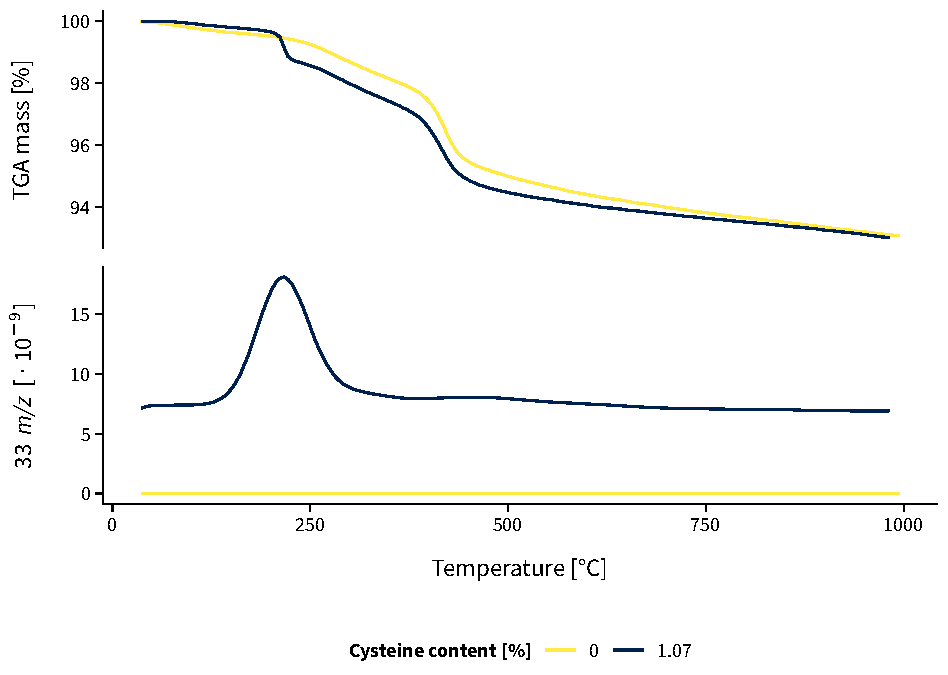
\includegraphics[width=\textwidth]{figures/cysteine-comparison}
	\caption[Exemplary \ac{tga} curves and \SI{33}{\mz} signals of \ac{pet} in soil with and without \textsc{dl}-cysteine as internal standard.]{Exemplary \ac{tga} curves and \SI{33}{\mz} signals of \ac{pet} in soil with and without addition of \textsc{dl}-cysteine (\SI{1.07}{\percent}) as internal standard.}
	\label{fig:cysteine-comparison}
\end{figure}

\begin{figure}
	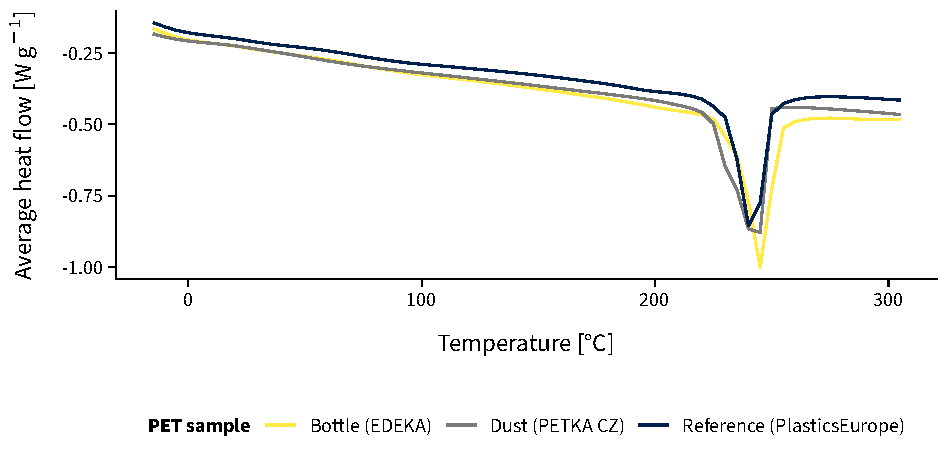
\includegraphics[width=\textwidth]{figures/dsc}
	\caption[Comparison of characteristic melting points of bulk \ac{pet} from a water bottle, ground \ac{pet} recyclate, and \iac{pet} reference.]{Comparison of characteristic melting points (averages of triplicate \ac{dsc} measurements) of bulk \ac{pet} from a water bottle, ground \ac{pet} recyclate, and \iac{pet} reference.}
	\label{fig:dsc}
\end{figure}

\begin{figure}
	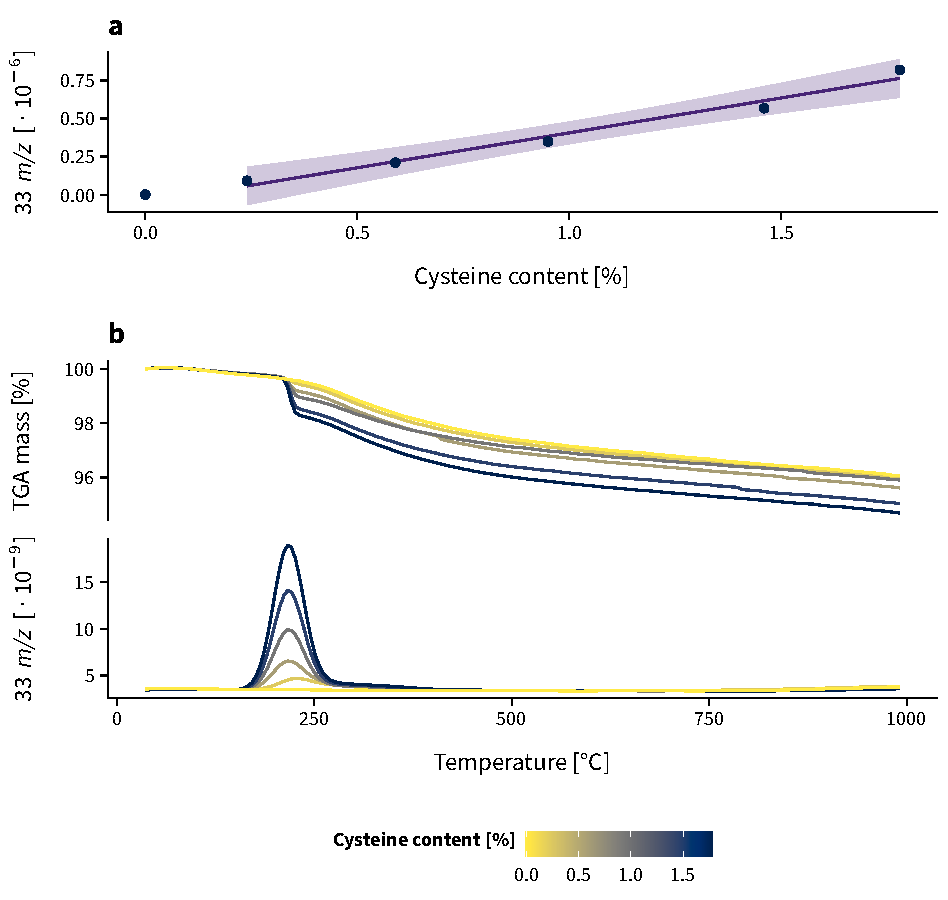
\includegraphics[width=\textwidth]{figures/cysteine-tests}
	\caption[Linear response of \ch{SH-} evolving from \textsc{dl}-cysteine pyrolysis in soil with corresponding \acs{tga} curves.]{(a) Linear response of \ch{SH-} (\SI{33}{\mz}) evolving from \textsc{dl}-cysteine pyrolysis in soil (adj. $R^2$ = \num{0.969}, \acs{rse} = \SI{8.96}{\percent}) with corresponding (b) \acs{tga} curves.}
	\label{fig:cysteine-tests}
	\forceversofloat
\end{figure}

\begin{figure*}
	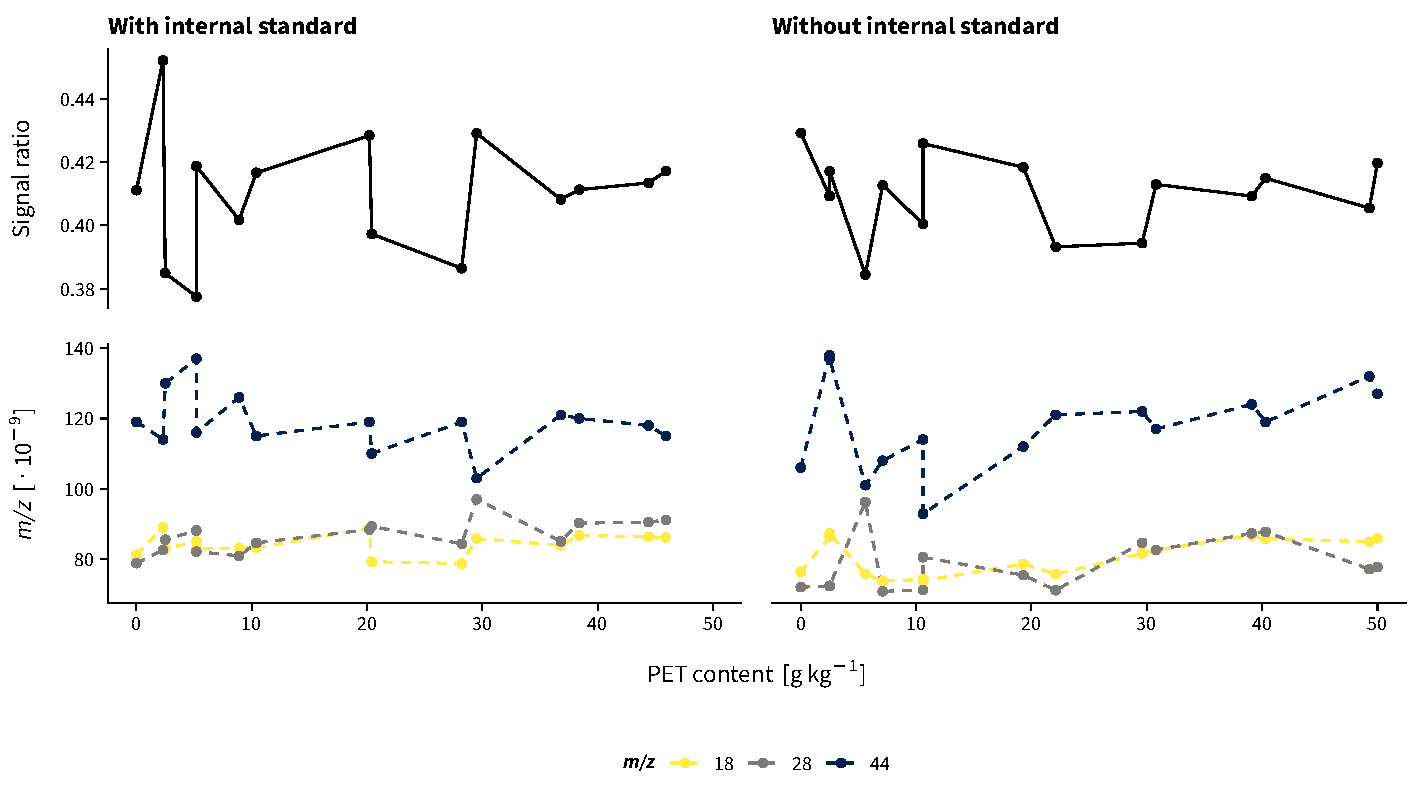
\includegraphics[width=\textwidth]{figures/control-measurements}
	\caption[Integrals of \ch{H2O}, \ch{CO}, and \ch{CO2} from control calcium oxalate hydrate pyrolyses after analyzing \ac{pet}-spiked soil.]{Integrals of \ch{H2O} (\SI{18}{\mz}), \ch{CO} (\SI{28}{\mz}), and \ch{CO2} (\SI{44}{\mz}) from control calcium oxalate hydrate pyrolyses after analyzing \acs{pet}-spiked soil; signal ratio = \SI{18}{\mz} / (\SI{28}{\mz} + \SI{44}{\mz}).}
	\label{fig:control-measurements}
	\forceversofloat
\end{figure*}

\begin{figure}
	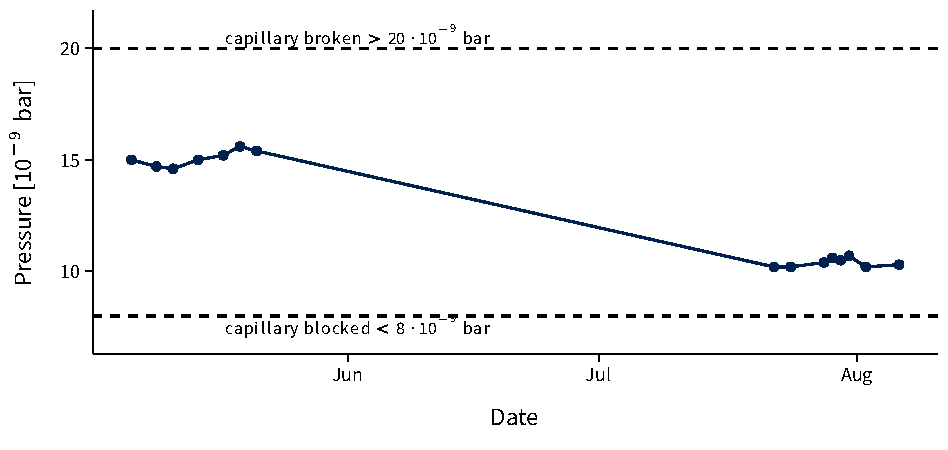
\includegraphics[width=\textwidth]{figures/tga-capillary-pressure}
	\caption{Pressure measurements in the \ac{tga} capillary during analyses.}
	\label{fig:tga-capillary-pressure}
\end{figure}

% !TeX spellcheck = en_US

\chapter{Supporting Information on the Screening Study}
\label{ap:screening}

\begin{figure*}
	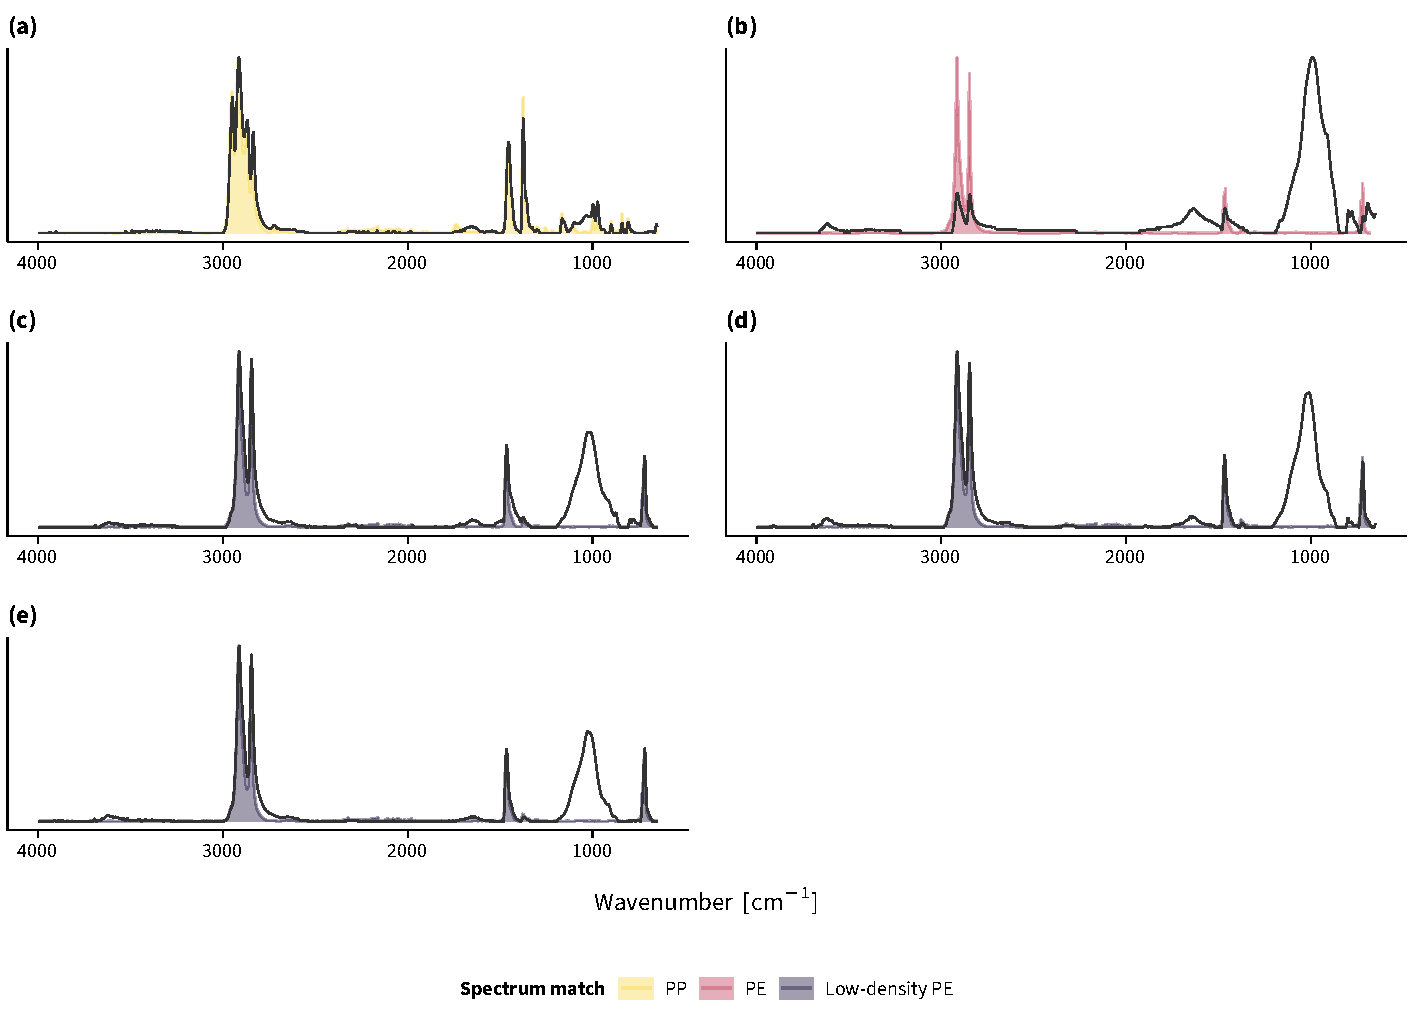
\includegraphics[width=\textwidth]{figures/ftir-covers}
	\caption[Exemplary \ac{ftir} spectra of the agricultural plastic covers on site.]{Exemplary \ac{ftir} spectra of (a) the \ac{pp} fleece from site 1, (b) the \ac{pe} mulch from sites 2 and 3, (c) the \ac{pe} fleece and (d) \ac{pe} perforated foil from sites 4 and 5, and (e) the \ac{pe} perforated foil from site 8. The measured \ac{ftir} spectra are in gray; the colored shades depict the respective Open Specy library match.}
	\label{fig:ftir-covers}
\end{figure*}

\begin{figure*}
	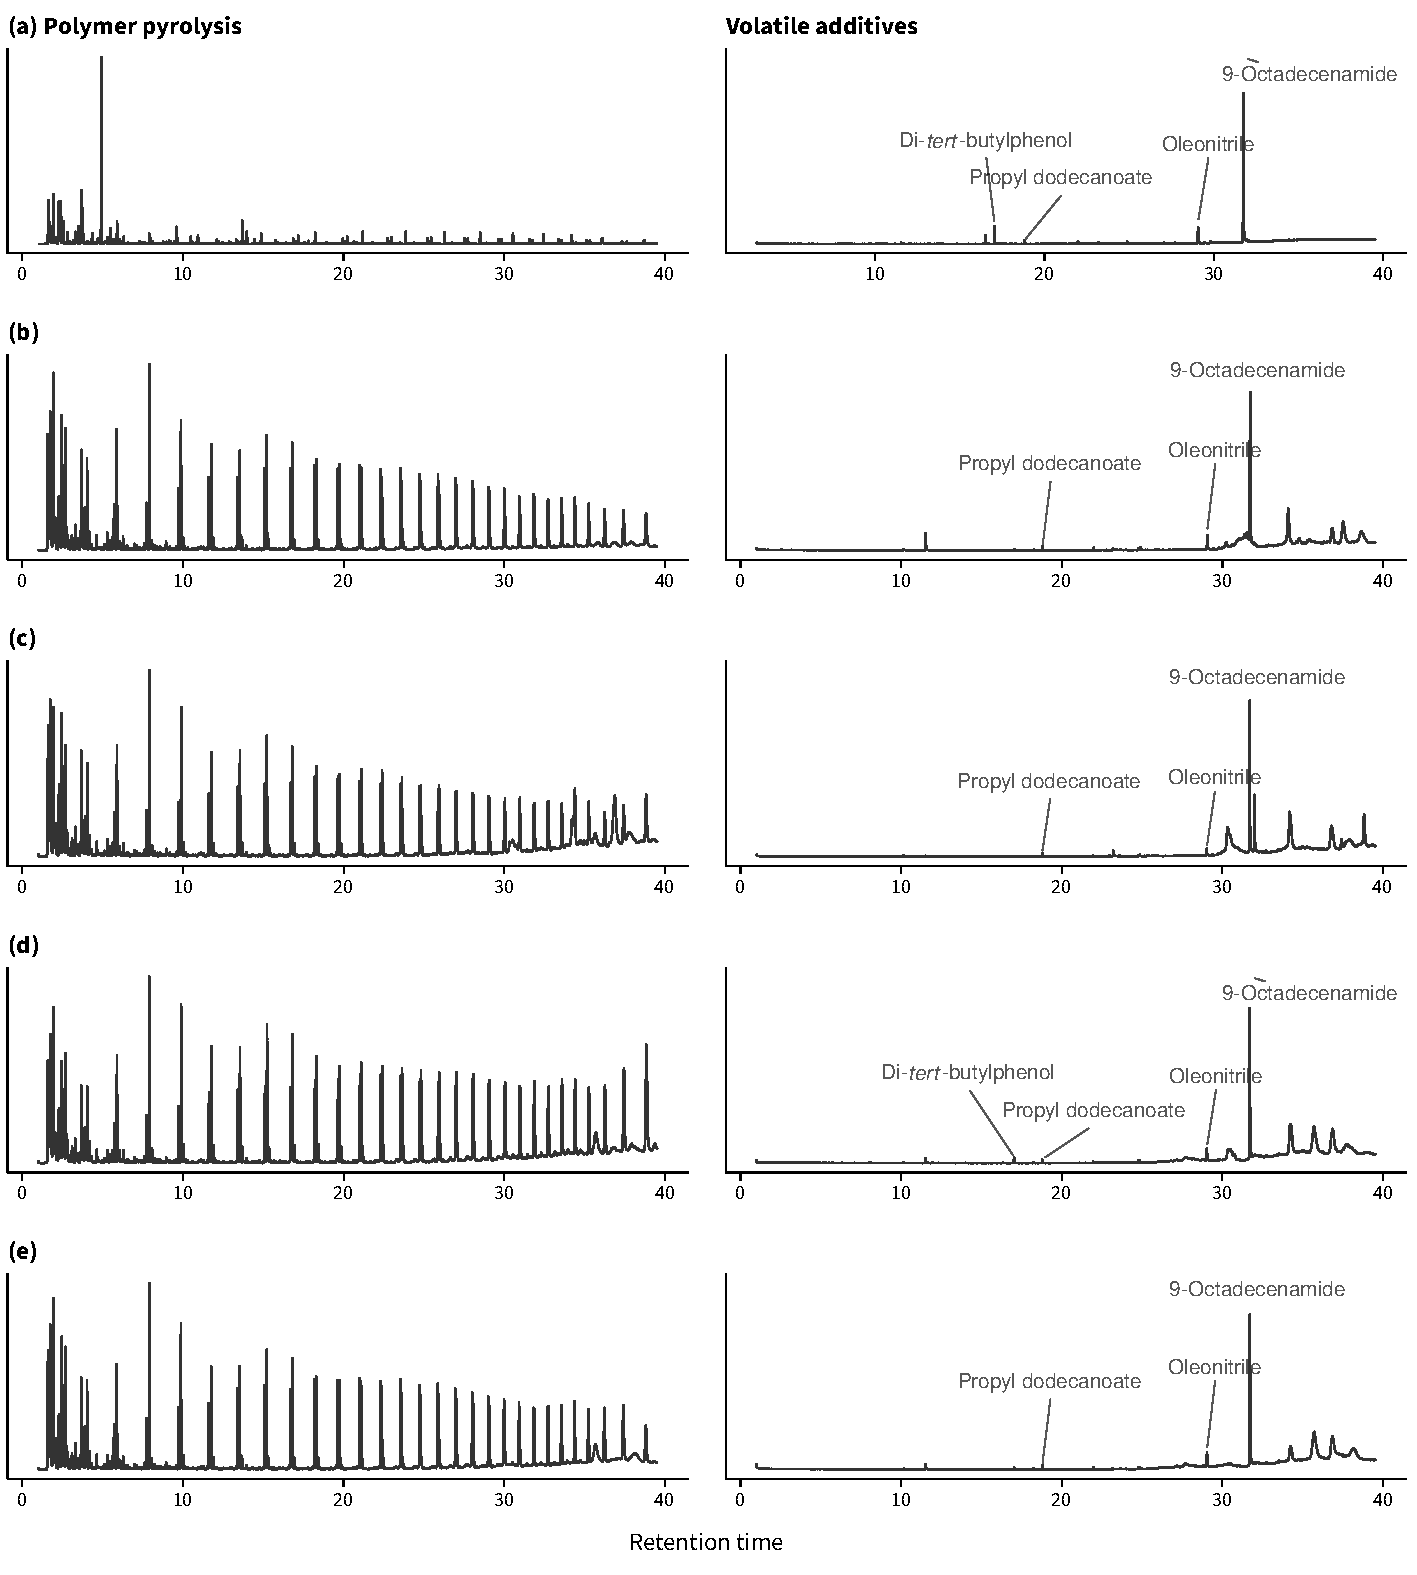
\includegraphics[width=\textwidth]{figures/py-covers}
	\caption[Exemplary chromatograms of polymer pyrolyses and thermal desorptions of polymer additives of the agricultural plastic covers.]{Exemplary chromatograms of polymer pyrolyses (\SI{750}{\degreeCelsius}, left) and thermal desorptions (\SI{300}{\degreeCelsius}, right) of polymer additives; (a) \ac{pp} fleece from site 1, (b) \ac{pe} mulch from sites 2 and 3, (c) \ac{pe} fleece and (d) \ac{pe} perforated foil from sites 4 and 5, and (e) \ac{pe} perforated foil from site 8; see Figure~\protect\ref{fig:ms-covers} for mass spectra.}
	\label{fig:py-covers}
	\forceversofloat
\end{figure*}

\begin{figure*}[p]
	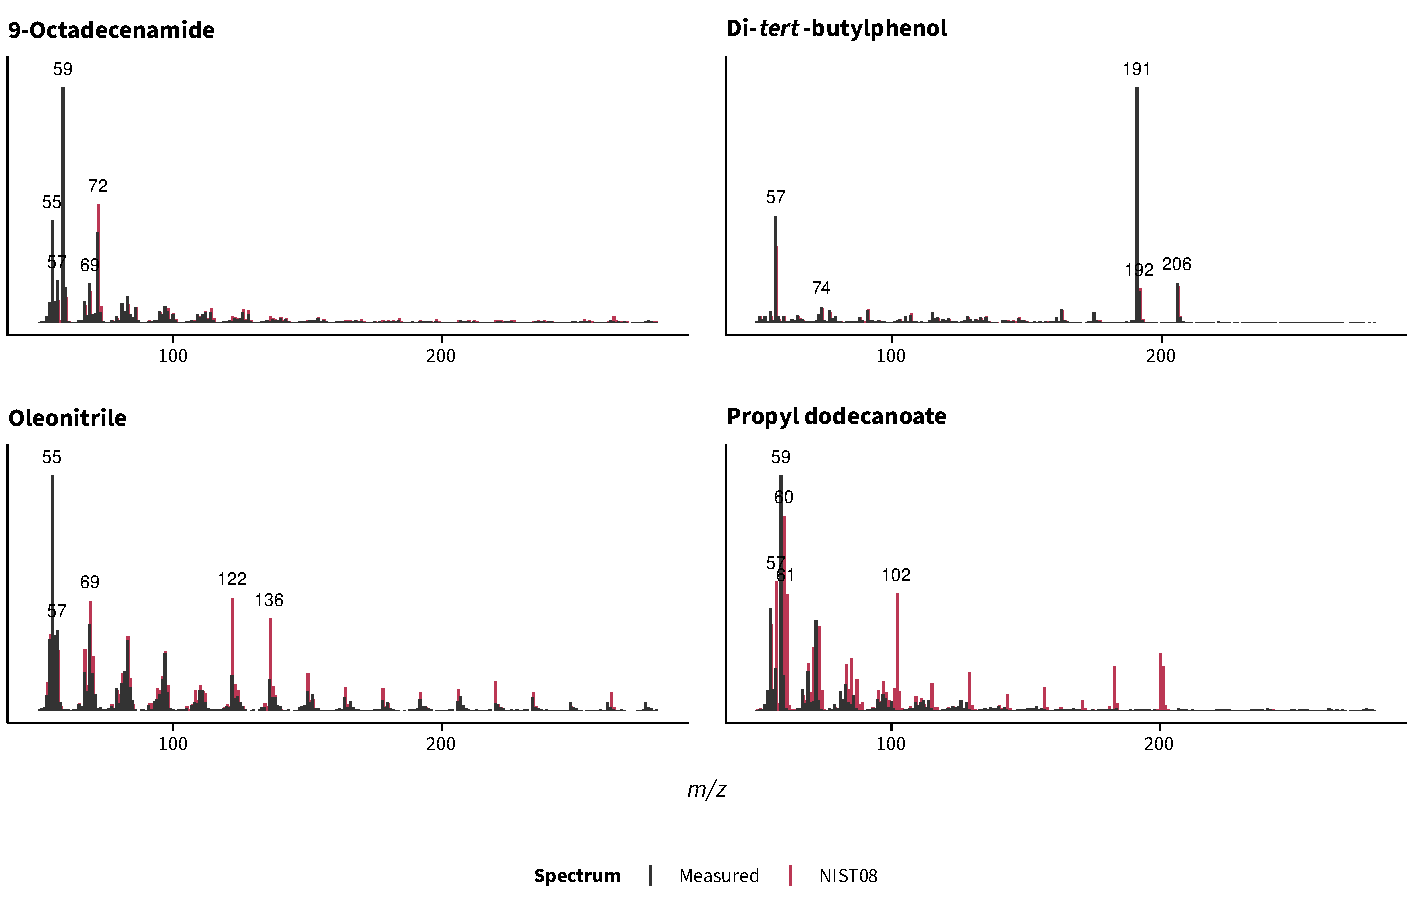
\includegraphics[width=\textwidth]{figures/ms-covers}
	\caption[Mass spectra and NIST08 library matches of the identified polymer additives.]{Mass spectra and NIST08 library matches of the identified polymer additives that thermally desorbed from the agricultural films; see Figure~\protect\ref{fig:py-covers} for chromatograms.}
	\label{fig:ms-covers}
\end{figure*}

\clearpage

\begin{figure*}[p]
	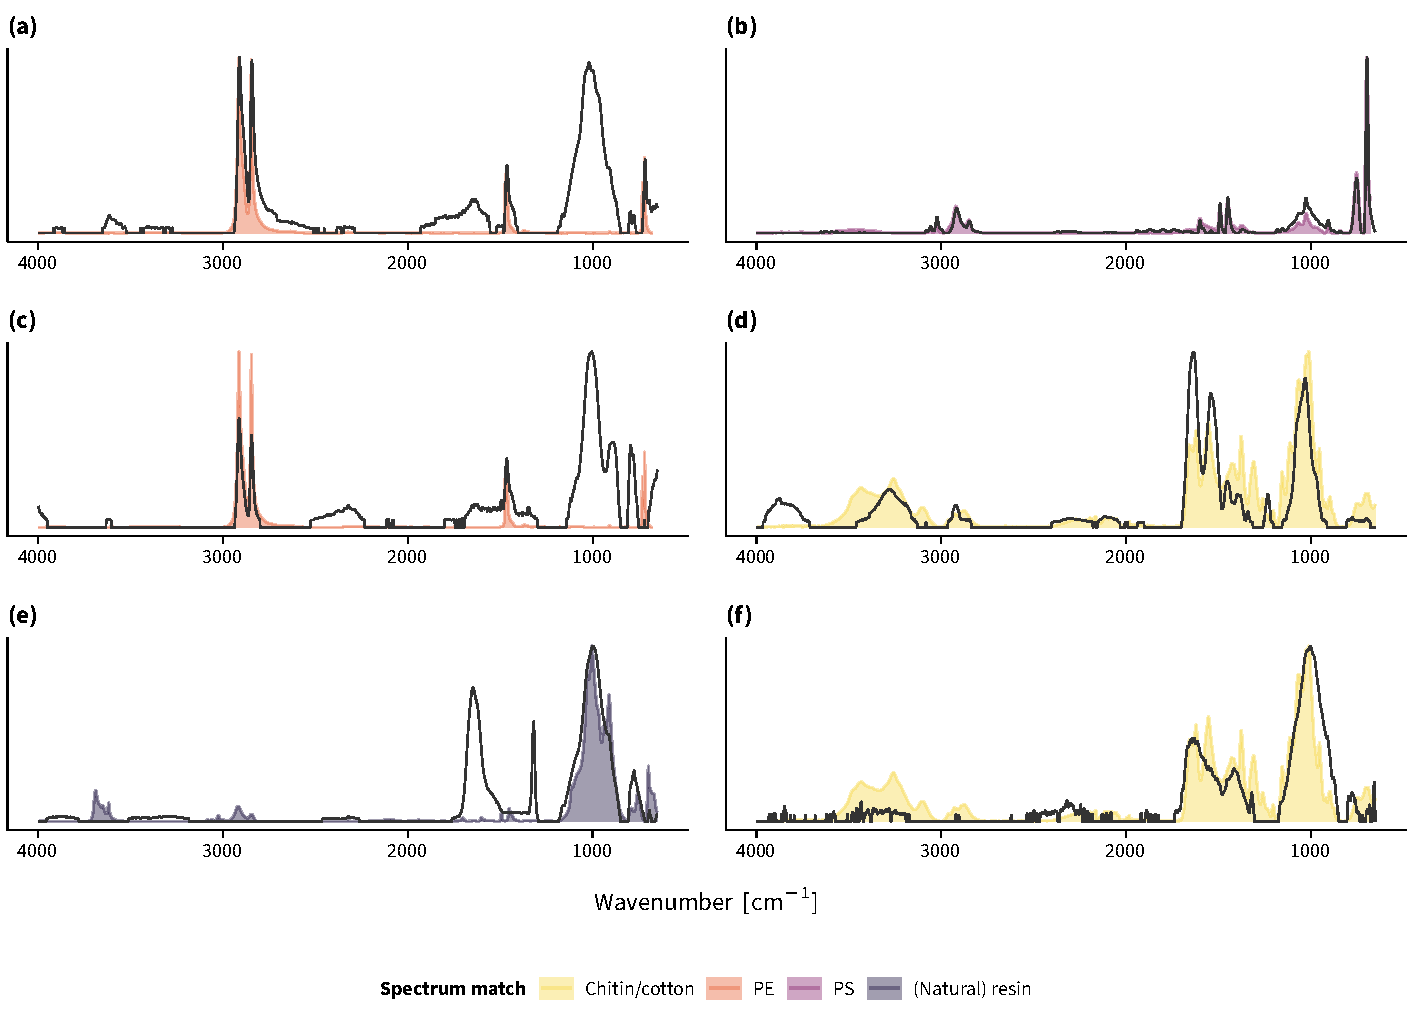
\includegraphics[width=\textwidth]{figures/ftir-debris}
	\caption[\Ac{ftir} spectra of the debris shown in Figure~\protect\ref{fig:visual-items}.]{\Ac{ftir} spectra of the debris shown in Figure~\protect\ref{fig:visual-items}; (a) \ac{pe} film and (b) \ac{ps} fragment from the field center of site 5, (c) \ac{pe} film and (d) chitin shell from the field center of site 6, and (e) resin or natural fragment and (f) cotton fiber from the field edge of site 7. The measured \ac{ftir} spectra are in gray; the colored shades depict the respective Open Specy library match.}
	\label{fig:ftir-debris}
\end{figure*}

\clearpage

\begin{figure*}[p]
	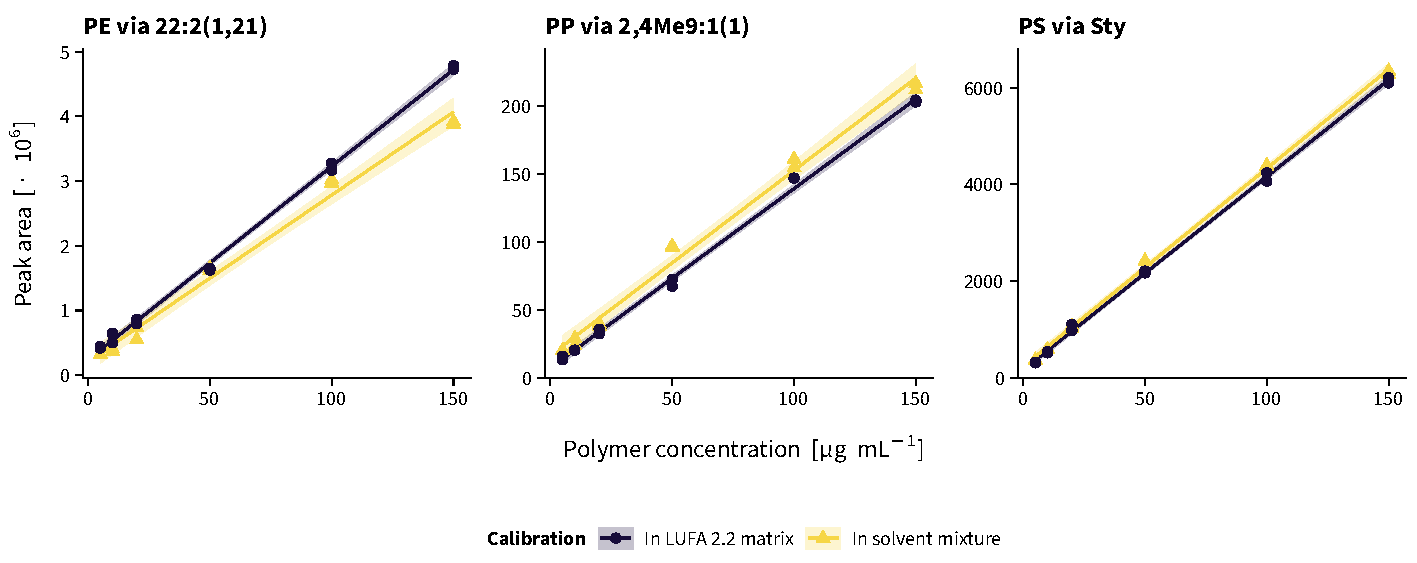
\includegraphics[width=\textwidth]{figures/matrix-match}
	\caption{\Ac{py-gc-ms} calibration in solvent \textit{p}-xylene/\ac{tcb} and in LUFA 2.2 matrix compared.}
	\label{fig:matrix-match}
	\forcerectofloat
\end{figure*}

% !TeX spellcheck = en_US

\chapter{Solubility Tests}
\label{ap:solubility-tests}

\begin{table}
	\centering\footnotesize
	\caption[\Ac{pe} solubility tests in \ac{tcb} and \textit{p}-xylene/\ac{tcb}.]{Testing the visual solubility of an ultra high-density \ac{pe}\textsuperscript{\textdagger} in \ac{tcb} at \SI{120}{\degreeCelsius} and in a 1:1-mixture (v+v) of \textit{p}-xylene and \ac{tcb} at \SI{150}{\degreeCelsius} after cooling down to room temperature. The used ultra high-density \ac{pe} was found to be particularly difficult to dissolve in comparison to low-density \ac{pe}, \ac{pp}, and \ac{ps}.}
	\label{tab:solubility-tests}
	\begin{tabular}{S[table-format = 4]ll}
		\toprule
		{\Ac{pe}\textsuperscript{\textdagger} concentration} & {in \ac{tcb}} & {in \textit{p}-xylene/\ac{tcb}} \\
		{[\si{\micro\gram\per\milli\liter}]} \\
		\midrule
		500 & gel formation & dissolved \\
		1000 & gel formation & dissolved \\ 
		1500 & gel formation & dissolved \\
		2000 & gel formation & refraction anomaly \\
		2500 & gel formation & refraction anomaly \\
		3000 & gel formation & gel formation \\
		3500 & gel formation & gel formation \\
		4000 & gel formation & gel formation \\
		\bottomrule
		\multicolumn{3}{p{.6\textwidth}}{\textsuperscript{\textdagger} \foreignlanguage{ngerman}{Bundesanstalt für Materialforschung und -prüfung}, Berlin, Germany.}
	\end{tabular}
\end{table}
\cleardoublepage

\backmatter
\pagenumbering{Roman}

% TODO: Check for short captions
\addcontentsline{toc}{chapter}{List of Figures}
\listoffigures

\addcontentsline{toc}{chapter}{List of Tables}
\listoftables

\printacronyms[name = List of Abbreviations, heading = chapter, template = thesis]

% !TeX spellcheck = en_US

\chapter{Electronic Supplement}

All text files, data, and code to reproduce data processing, plotting, and statistical tests are available at the following link\slash QR code:

\begin{figure}[!h]
	\centering
	\qrcode[height=2.5cm,padding]{https://git.io/Ja2DV}

	{\hypersetup{hidelinks}\url{https://git.io/Ja2DV}}
\end{figure}

\subsection*{This Includes the Following Files and Folders}

\begin{description}[leftmargin=8.5em,style=nextline,font=\normalfont\ttfamily]
	\item[README.md] Readme file
	\item[thesis.pdf] Dissertation as PDF file
	\item[thesis.tex] Dissertation as editable \LaTeX\ source file including all thesis contents from the following subdirectories: \texttt{frontbackmatter/}, \texttt{chapters/}, \texttt{appendices/}
	\item[proposal.pdf] Thesis proposal as PDF file
	\item[proposal.tex] Thesis proposal as editable \LaTeX\ source file
	\item[references.bib] Complete bibliographical data of the references cited
	\item[figures/] Figures
	\item[tables/] Tables
	\item[supplements/] Supplemental (raw) data and code
	\item[cv/] Curriculum vitae
	\item[defense/] Slides of the thesis defense
\end{description}

\clearpage

% !TeX spellcheck = en_US

\newgeometry{left=82.4mm,asymmetric}
\reversemarginpar
\fancyhfoffset[RO]{0mm}

\chapter[Curriculum Vitae]{Zacharias Steinmetz}

	\begin{cv}

	\info{\vspace*{0em}
		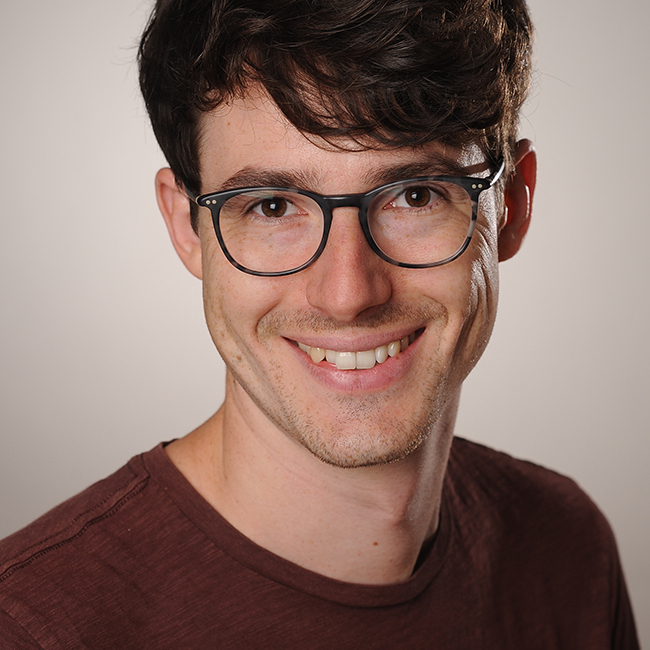
\includegraphics[width=.6\marginparwidth,,cfbox=black 0.75pt 0pt]{cv/portrait}}

	\vspace{.5em}

	\noindent
	\begin{minipage}{0.5\linewidth}
		Horststr. 157\\
		76829 Landau\\
		Germany
	\end{minipage}
	\begin{minipage}{0.5\linewidth}
		\begin{itemize}[left=.65em, noitemsep]
			\item[\color{InfRd}\envelope] \email{info@zsteinmetz.de}
			\item[\href{https://orcid.org/0000-0001-6675-5033}{\orcid}]
			\href{https://orcid.org/0000-0001-6675-5033}{0000-0001-6675-5033}
			\item[\href{https://publons.com/researcher/AAC-9025-2020/}{\publons}]
			\href{https://publons.com/researcher/AAC-9025-2020/}{AAC-9025-2020}
		\end{itemize}
	\end{minipage}

	\vspace{1em}
	\noindent Born September 23, 1989, in Frankfurt am Main (Germany) \\
	\noindent Nationality: German

	\vspace{2em} % Extra white space


	%-------------------------------------------------------------------------------

	\heading{Education}

	\entry{10/2013--11/2016}{M.Sc. Ecotoxicology}{University of Koblenz--Landau (Germany)}
	\desc{\info{Thesis title}%
		``Tracking the transformation of phenolic compounds in soil with compound-specific stable carbon isotope analysis.''
		\newline
		\info{Final grade}1.2
	}

	\entry{10/2010--11/2013}{B.Sc. Environmental Sciences}{University of Koblenz--Landau (Germany)}
	\desc{\info{Thesis title}%
		``Persistence of chemical and biological effects of olive mill wastewater seasonally applied to loessial olive orchard soil.''
		\newline
		\info{Final grade}1.5
	}

	\entry{8/2000--7/2009}{Abitur}{Christian-Wirth-Gymnasium Usingen (Germany)}
	\desc{\info{Advanced courses}%
		Chemistry and mathematics
	}

	%-------------------------------------------------------------------------------

	\heading{Research and Work Experience}

	\entry{12/2016--present}{Research Associate}{University of Koblenz--Landau (Germany)}

	\desc{%
		Scrutinizing microplastic fate in agricultural soil using \ac{py-gc-ms}.
	}

	\entry{8/2019}{Guest Researcher}{LUT (Finland)}
	\desc{%
		Exchanging knowledge on microplastic extraction from soil and sediment and Raman spectroscopy.
	}

	\entry{4/2015--10/2015}{Student Employee}{RIFCON GmbH (Germany)}
	\desc{%
		Conducting individual-based ecological modeling and crop modeling in cooperation with Alterra (Netherlands).
	}

	\entry{6/2014--8/2014}{Intern}{MITOX Consultants/Eurofins (France)}
	\desc{%
		Assisting in ecotoxicological (semi-)field trials on non-target arthropods.
	}

	\entry{6/2013--8/2013}{Guest Researcher}{Agricultural Research Organization (Israel)}

	%-------------------------------------------------------------------------------

	\heading{Funding}

	\entry{}{Travel Grants \num{>1000} Euro}{}
	\desc{%
		%\info{5/2020}Ireland (University-intern research fund)\hfill{\small 550 Euro} \\
		\info{8/2019}Finland (Erasmus+)\hfill{\small 1895 Euro}\\
		\info{1/2018}Chile (Erasmus+)\hfill{\small 3020 Euro}
	}
	\entry{}{Scholarships}{}
	\desc{%
		\info{8/2016--12/2016}``AufLand'' publication grant for junior scientists\hfill{\small 3000 Euro}\\
		\info{3/2015--9/2016}\foreignlanguage{ngerman}{Studienstiftung des deutschen Volkes}\hfill{\small 7905 Euro}
	}

	%-------------------------------------------------------------------------------

	\heading{Teaching Experience}

	\entry{10/2021--present}{\foreignlanguage{ngerman}{Laborübungen Umweltanalytik}}{Co-supervisor}

	\entry{10/2017--present}{\foreignlanguage{ngerman}{Methoden der Natur- und Umweltwissenschaften}}{Associate lecturer}

	\entry{12/2016--present}{Advanced Environmental Chemistry}{Lecturer}

	\entry{10/2015--2/2016}{R for Beginners}{Teaching assistant}

	%-------------------------------------------------------------------------------

	\heading{Administrative Experience}

	\entry{12/2016--present}{Staff Representative}{University of Koblenz--Landau (Germany)}
	\desc{In various panels including the committee on educational affairs and the PhD committee of the faculty council of Environmental and Natural Sciences.}

	\entry{1/2014--12/2015}{Elected Student Representative}{University of Koblenz--Landau (Germany)}
	\desc{Faculty council of Environmental and Natural Sciences.}

	%-------------------------------------------------------------------------------

	\heading{Skills}

	\desc{\info{German}native
		\newline
		\info{English}proficient (10 school years, 1 year practice in the Philippines)
		\newline
		\info{French}basic (5 school years)
	}

	\desc{\info{Analytics}\Ac{py-gc-ms}, \ac{gc-ms}, GC/IRMS, GC/FID, HPLC, and \ac{ftir}--\ac{atr} using OpenChrom, Thermo Xcalibur, LCquan, and Isodat, Agilent ChemStation, and Open Specy for data analysis.
	}

	\desc{%
		\info{Computer skills}Advanced in R statistics and office applications
		\newline
		Competent in GIS (QGIS, GRASS), Python, Linux shell, \LaTeX, git
		\newline
		Basic knowledge of Docker, SQL, HTML, and PHP.
		\newline

		\noindent\info{Software development}%
		Visit \href{https://github.com/zsteinmetz}{\faIcon{github} github.com/zsteinmetz} for an overview of my open-source software development.
	}

	%-------------------------------------------------------------------------------

	\heading{Selected Scientific Contributions}

	\desc{\small%
		\info{Peer-reviewed articles not listed in \nameref{ch:author-contributions}}
		\begin{refsection}[articles]
			\nocite{*}
			\printbibliography[heading=subbibliography,title=\vspace{-2.925\baselineskip}]
		\end{refsection}

		\vspace{.4\baselineskip}

		\noindent See \href{https://scholar.google.de/citations?user=klQROs4AAAAJ}{\googlescholar\ scholar.google.de/citations?user=klQROs4AAAAJ} for a complete publication list.

	}

	\desc{\small%
		\info{Referee}
		\textit{Journal of Analytical and Applied Pyrolysis}, \textit{Science of the Total Environment}, \textit{Environmental Pollution}, \textit{Polymers}, \textit{Frontiers in Environmental Science}.
	}

	\desc{%
		\info{Invited speaker}
		\begin{refsection}[talks]
			\nocite{*}
			\printbibliography[heading=subbibliography,title=\vspace{-2.925\baselineskip}]
		\end{refsection}
	}

	%-------------------------------------------------------------------------------

	\vspace{2em}

	\noindent
	\end{cv}

\normalmarginpar
\restoregeometry

\clearpage
\thispagestyle{empty}
\begin{fullwidth}
	~\vfill
	\centering\faIcon{jedi-order}
\end{fullwidth}

\cleardoublepage

\end{document}
